%% LyX 2.0.3 created this file.  For more info, see http://www.lyx.org/.
%% Do not edit unless you really know what you are doing.
\documentclass[11pt,a4paper,american,english]{article}
\usepackage[T1]{fontenc}
\usepackage[latin9]{inputenc}
\usepackage{listings}
\pagestyle{empty}
\setcounter{tocdepth}{2}
\setlength{\parskip}{\medskipamount}
\setlength{\parindent}{0pt}
\synctex=-1
\usepackage{color}
\usepackage{babel}
\usepackage{array}
\usepackage{longtable}
\usepackage{varioref}
\usepackage{prettyref}
\usepackage{float}
\usepackage{wrapfig}
\usepackage{booktabs}
\usepackage{units}
\usepackage{url}
\usepackage{pdfpages}
\usepackage{multirow}
\usepackage{amsmath}
\usepackage{amssymb}
\usepackage{makeidx}
\makeindex
\usepackage{graphicx}
\usepackage{setspace}
\PassOptionsToPackage{normalem}{ulem}
\usepackage{ulem}
\usepackage{nomencl}
% the following is useful when we have the old nomencl.sty package
\providecommand{\printnomenclature}{\printglossary}
\providecommand{\makenomenclature}{\makeglossary}
\makenomenclature
\usepackage[unicode=true,
 bookmarks=true,bookmarksnumbered=false,bookmarksopen=true,bookmarksopenlevel=2,
 breaklinks=true,pdfborder={0 0 0},backref=false,colorlinks=true]
 {hyperref}
\hypersetup{pdftitle={ImageJ User Guide },
 pdfauthor={Tiago Ferreira \& Wayne Rasband},
 pdfsubject={ImageJ 1.46 Handbook},
 pdfkeywords={ImageJ, Fiji, Scientific Digital Image Processing},
 hyperindex=true, linkcolor={black!65}, citecolor={black!65}, urlcolor={blue!40!black}, pdfstartview=FitH, pdfpagelayout=OneColumn}

\makeatletter

%%%%%%%%%%%%%%%%%%%%%%%%%%%%%% LyX specific LaTeX commands.
\pdfpageheight\paperheight
\pdfpagewidth\paperwidth

\newcommand{\noun}[1]{\textsc{#1}}
\DeclareRobustCommand*{\lyxarrow}{%
\@ifstar
{\leavevmode\,$\triangleleft$\,\allowbreak}
{\leavevmode\,$\triangleright$\,\allowbreak}}
%% Special footnote code from the package 'stblftnt.sty'
%% Author: Robin Fairbairns -- Last revised Dec 13 1996
\let\SF@@footnote\footnote
\def\footnote{\ifx\protect\@typeset@protect
    \expandafter\SF@@footnote
  \else
    \expandafter\SF@gobble@opt
  \fi
}
\expandafter\def\csname SF@gobble@opt \endcsname{\@ifnextchar[%]
  \SF@gobble@twobracket
  \@gobble
}
\edef\SF@gobble@opt{\noexpand\protect
  \expandafter\noexpand\csname SF@gobble@opt \endcsname}
\def\SF@gobble@twobracket[#1]#2{}
%% Because html converters don't know tabularnewline
\providecommand{\tabularnewline}{\\}
%% A simple dot to overcome graphicx limitations
\newcommand{\lyxdot}{.}

\floatstyle{ruled}
\newfloat{infobox}{htb}{loi}
\providecommand{\infoboxname}{Noteworthy}
\floatname{infobox}{\protect\infoboxname}

%%%%%%%%%%%%%%%%%%%%%%%%%%%%%% Textclass specific LaTeX commands.
\makeatletter
  %%%%%%%%%%%% Page Layout
    % We want a screen reading pdf without odd/even margin assymetry and a booklet-like print
    % version created by pdfpages. For the booklet version we will place the marginal todonotes on
    % the outer margin, saving space in the inner margin of the booklet. We will use the option
    % <twoside> to alternate marginpars, then eliminate symmetry with the geometry package. We will
    % increase <textwidth> and <textheight>. NB: fancyhdr must be loaded after geometry parameters!
    \usepackage[a4paper, twoside, hmarginratio={1:1},margin=2.58cm]{geometry}
    \usepackage{mparhack} % correct the notorious bug of misplaced mpar on top of page
    %\reversemarginpar % force all subsequent marginal notes to be put on the opposite side

  %%%%%%%%%%%% File size
    %\pdfcompresslevel=9 % default: 9
    %\pdfminorversion=5 % increase PDF version so that compression can be used, default: 5
    %\pdfobjcompresslevel=2 % compress non-stream objects, default: 2
    %\usepackage{cmap} % use real Unicode characters instead of TeX compounds for non-ASCII chars

  %%%%%%%%%%%% General
    \usepackage{ifthen}
    \usepackage{microtype} % micro-typographic extensions of pdfTEX
    \usepackage{sectsty} % sections font control
    \usepackage{appendix} % appendices control
    \usepackage[amssymb,textstyle]{SIunits} % get the upright'\micro'
    \usepackage{textcomp} % e.g., to produce \textquotesingle

  %%%%%%%%%%%% Fix for Acrobat Readers 
    % By default Acrobat Readers use DeviceCMYK. At least with AR 8 and 9, converted RGB colors are
    % shifted and ill rendered, so we'll make sure AR will use DeviceRGB
    \pdfpageattr{/Group <</S /Transparency /I true /CS /DeviceRGB>>}

  %%%%%%%%%%%% Adjust headers
    \usepackage{fancyhdr}
    \pagestyle{fancy}
    %%% Get Dates to place in footer
    \newcommand{\revisiondate}{{\the\year/\/\two@digits{\the\month}/\/\two@digits{\the\day}}}
    %%% Adjust parameters
    \renewcommand{\headrulewidth}{0pt} %default is 0.4pt? 
    \fancyhead{}
    \renewcommand{\sectionmark}[1]{\markboth{#1}{}}
    \renewcommand{\subsectionmark}[1]{\markright{#1}{}}
    \rhead{\scriptsize\rightmark}
    \lhead{\scriptsize\leftmark}
    \fancyfoot[R]{\scriptsize{}Last updated: \revisiondate}
    %\fancyfoot[C]{}\fancyfoot[R]{\scriptsize\thepage}

  %%%%%%%%%%%%  Adjust Floats
    \usepackage[below]{placeins} % floats are not placed before the section, less demanding than strict
    %%% Adjust captions. Default preset for caption skip is 10pt
    \usepackage[font=small]{caption} % textformat=period
    \captionsetup[figure]{labelformat=empty,position=bottom,skip=5pt}
    \captionsetup[table]{labelformat=empty,position=top,skip=5pt}
    %%% Center all tables and figure floats
    \renewenvironment{figure}[1][]{%
        \ifthenelse{\equal{#1}{}}{\@float{figure}}{\@float{figure}[#1]}\centering
    }{\end@float}
    \renewenvironment{table}[1][]{%
        \ifthenelse{\equal{#1}{}}{\@float{table}}{\@float{table}[#1]}\centering
    }{\end@float}

  %%%%%%%%%%%%  Adjust Listings
    \usepackage{listings, xcolor}
    \colorlet{lstfcolor}{gray}% color of frame to be used in caption and lstset
    \colorlet{lstbcolor}{lstfcolor!10} % color of background to be used in lset
  
    % Define a new caption style for listings: We'll insert a tcolorbox to match 'noteworthy' floats
    \DeclareCaptionFormat{listing}{
        \begin{tcolorbox}[coltext=white,colback=lstfcolor,colframe=lstfcolor,boxsep=0pt,top=2pt,bottom=2pt,left=4pt,boxrule=0.4mm]
        {#1#2#3}
        \end{tcolorbox}\vspace*{-7.6pt}
    }
    % Adjust lstlisting caption
    \captionsetup[lstlisting]{%
        format=listing, labelformat=parens, font={small,bf}, labelsep=space, listformat=parens, singlelinecheck=false
    }
    \providecommand*{\lstlistingname}{} %\footnotesize\textsc{Macro}
    \renewcommand*{\lstlistingname}{}   %\footnotesize\textsc{Macro}
    \lstdefinelanguage{ijm} {
        language= java,
      % comments: italic green in Fiji
        commentstyle=\slshape\color[RGB]{0,200,0},
      % strings: magenta(?) in Fiji
        stringstyle=\color[RGB]{140,0,140},
      % operators: brown(?) in Fiji
        otherkeywords={+,-,=,<,!,\&},
        keywordstyle=\color[RGB]{130,60,0},
      % digits: gray(?) in Fiji
        alsoletter={1234567890},
        emph={[3]1,2,3,4,5,6,7,8,9,0,16,32,111,121,132,255,256},
        emphstyle=[3]\color[RGB]{50,50,50},
      % statements: bold blue in Fiji
        emph={[2]var,macro,function,return,true,false,if,then,else,for,while,do,length},
        emphstyle=[2]\color[RGB]{0,0,200}\bf,
      %IJ v1.46 built-in macro functions: golden(?) in Fiji
        emph={abs, acos, Array.concat, Array.copy, Array.fill, Array.getStatistics, Array.print, Array.rankPositions, Array.reverse, Array.slice, Array.sort, Array.trim, asin, atan, atan2, autoUpdate, beep, bitDepth, calibrate, call, changeValues, charCodeAt, close, cos, d2s, Dialog.create, Dialog.addMessage, Dialog.addString, Dialog.addNumber, Dialog.addSlider, Dialog.addCheckbox, Dialog.addCheckboxGroup, Dialog.addChoice, Dialog.addHelp, Dialog.setInsets, Dialog.show, Dialog.getString, Dialog.getNumber, Dialog.getCheckbox, Dialog.getChoice, doCommand, doWand, drawLine, drawOval, drawRect, drawString, dump, endsWith, eval, exec, exit, exp, Ext, File.append, File.close, File.dateLastModified, File.delete, File.directory, File.exists, File.getName, File.getParent, File.isDirectory, File.lastModified, File.length, File.makeDirectory, File.name, File.nameWithoutExtension, File.open, File.openAsString, File.openAsRawString, File.openUrlAsString, File.openDialog, File.rename, File.saveString, File.separator, fill, fillOval, fillRect, Fit.doFit, Fit.rSquared, Fit.p, Fit.nParams, Fit.f, Fit.nEquations, Fit.getEquation, Fit.plot, Fit.logResults, Fit.showDialog, floodFill, floor, fromCharCode, getArgument, getBoolean, getBoundingRect, getCursorLoc, getDateAndTime, getDimensions, getDirectory, getDisplayedArea, getFileList, getHeight, getHistogram, getImageID, getImageInfo, getInfo, getLine, getList, getLocationAndSize, getLut, getMetadata, getMinAndMax, getNumber, getPixel, getPixelSize, getProfile, getRawStatistics, getResult, getResultLabel, getSelectionBounds, getSelectionCoordinates, getSliceNumber, getStatistics, getString, getStringWidth, getThreshold, getTime, getTitle, getValue, getVoxelSize, getVersion, getWidth, getZoom, IJ, deleteRows, getToolName, freeMemory, currentMemory, maxMemory, pad, redirectErrorMessages, renameResults, imageCalculator, indexOf, is, isActive, isKeyDown, isNaN, isOpen, lastIndexOf, lengthOf, lineTo, List.set, List.get, List.getValue, List.size, List.clear, List.setList, List.getList, List.setMeasurements, List.setCommands, log, makeEllipse, makeLine, makeOval, makePoint, makePolygon, makeRectangle, makeSelection, makeText, matches, maxOf, minOf, moveTo, newArray, newImage, newMenu, nImages, nResults, nSlices, open, Overlay.moveTo, Overlay.lineTo, Overlay.drawLine, Overlay.add, Overlay.setPosition, Overlay.drawRect, Overlay.drawEllipse, Overlay.drawString, Overlay.show, Overlay.hide, Overlay.hidden, Overlay.remove, Overlay.size, Overlay.removeSelection, Overlay.copy, Overlay.paste, parseFloat, parseInt, PI, Plot.create, Plot.setLimits, Plot.setFrameSize, Plot.setLineWidth, Plot.setColor, Plot.add, Plot.addText, Plot.setJustification, Plot.drawLine, Plot.show, Plot.update, Plot.getValues, pow, print, random, rename, replace, requires, reset, resetMinAndMax, resetThreshold, restorePreviousTool, restoreSettings, roiManager, round, run, runMacro, save, saveAs, saveSettings, screenHeight, screenWidth, selectionContains, selectionName, selectionType, selectImage, selectWindow, setAutoThreshold, setBackgroundColor, setBatchMode, setColor, setFont, setForegroundColor, setJustification, setKeyDown, setLineWidth, setLocation, setLut, setMetadata, setMinAndMax, setOption, setPasteMode, setPixel, setResult, setRGBWeights, setSelectionLocation, setSelectionName, setSlice, setThreshold, setTool, setupUndo, setVoxelSize, setZCoordinate, showMessage, showMessageWithCancel, showProgress, showStatus, sin, snapshot, split, sqrt, Stack.isHyperstack, Stack.getDimensions, Stack.setDimensions, Stack.setChannel, Stack.setSlice, Stack.setFrame, Stack.getPosition, Stack.setPosition, Stack.getFrameRate, Stack.setFrameRate, Stack.getFrameInterval, Stack.setFrameInterval, Stack.getUnits, Stack.setTUnit, Stack.setZUnit, Stack.setDisplayMode, Stack.getDisplayMode, Stack.setActiveChannels, Stack.getActiveChannels, Stack.swap, Stack.getStatistics, startsWith, String.resetBuffer, String.append, String.buffer, String.copy, String.copyResults, String.getResultsHeadings, String.paste, substring, tan, toBinary, toHex, toLowerCase, toolID, toScaled, toUnscaled, toString, toUpperCase, updateDisplay, updateResults, wait, waitForUser},%
        emphstyle=\color[RGB]{165,65,0},
      % other settings
        sensitive=true, upquote=true, showstringspaces=false,
    }
    \lstset{%
        language=ijm, float=htb, captionpos=t,
        frame=tblr, framerule=0.4mm, rulecolor=\color{lstfcolor},
        xleftmargin=13.15pt, framexleftmargin=9pt, framexrightmargin=-4.2pt,%
        backgroundcolor=\color{lstbcolor},
        numbers=left, numbersep=3pt, numberstyle=\tiny,
        breaklines=true, breakatwhitespace=true, breakindent=15pt,
        prebreak=\raisebox{0ex}[0ex][0ex]{\ensuremath{\hookleftarrow}},
        basicstyle=\footnotesize\ttfamily,
    }

  %%%%%%%%%%%%  Adjust Footnotes
    \usepackage[perpage,hang,flushmargin]{footmisc}
    % adjust footnoterule
    \addtolength{\skip\footins}{3mm}
    \renewcommand\footnoterule{\kern-3\p@\hrule\@width1\columnwidth\kern2.6\p@}
    % make arabic footnote marks inside minipages (to be used in tables)
    \let\thempfootnote\thefootnote
    % define an unnumbered footnote (without footmark)
    \def\blfootnote{\xdef\@thefnmark{}\@footnotetext}

  %%%%%%    Fix for hyperfootnotes
    % hyperfootnotes= false must be loaded as an option. it has no effect in the in hypersetup. As of this
    % writings LyX does not allow to load this option in the Document properties. This will impose it
    \toks@\expandafter{%
        \expandafter\ifHy@hyperfootnotes
            \@footnotemark
            \else \H@@footnotemark
            \fi}
    \xdef\@footnotemark{\the\toks@}%
    \let\footnotes@ve = \footnote
    \def\footnote{\Hy@hyperfootnotesfalse\footnotes@ve}

  %%%%%%%%%%%%  Adjust index
    \usepackage{multicol}
    \renewenvironment{theindex}{
        \if@twocolumn \@restonecolfalse \else \@restonecoltrue \fi
        \setlength{\columnseprule}{0pt}
        \setlength{\columnsep}{35pt}
        \flushleft
        \begin{multicols}{3}[\section*{\indexname}]
        %\markboth{\MakeUppercase\indexname}{\MakeUppercase\indexname}%
            \setlength{\parindent}{0pt}
            \setlength{\parskip}{0.3pt}
            \relax\let\item\@idxitem}%
        {\end{multicols}
        \if@restonecol\onecolumn\else\clearpage\fi}
    \renewcommand\@idxitem{\par\hangindent 20\p@}
    \renewcommand\subitem{\@idxitem \hspace*{10\p@}}
    \renewcommand\subsubitem{\@idxitem \hspace*{20\p@}}
    %\renewcommand\indexspace{\par \vskip 5\p@ \@plus5\p@ \@minus3\p@\relax}

  %%%%%%%%%%%%  Adjust Nomenclature
    \usepackage{nomencl}
    \renewcommand{\nomname}{List of Abbreviations and Acronyms}%
    \setlength{\nomlabelwidth}{.18\hsize}%
    \renewcommand{\nomlabel}[1]{#1 \dotfill}%
    \setlength{\nomitemsep}{3.6pt}%
    \renewcommand{\nomentryend}{;}%
    \renewcommand*\nompreamble{
        \setlength{\columnsep}{12mm} %width between the multicols columns
        \flushleft\footnotesize\begin{multicols*}{2}}%
    \renewcommand*\nompostamble{\end{multicols*}}%

  %%%%%%%%%%%%  Define the "Noteworthy" float
    % We could define a new type of float but we'll instead customize the default "ruled" style
    % (see http://en.wikibooks.org/wiki/LaTeX/Floats,_Figures_and_Captions)
    \usepackage{float}
    \usepackage{tcolorbox}
    \tcbuselibrary{skins} % loads tikz
    \usetikzlibrary{shadings,shadows}
    % Tweak the ruled style: hack a tcolorbox inside the float
    \colorlet{shadecolor}{green!15} %will be used by cellcolor in doc
    \renewcommand\floatc@ruled[2]{{\@fs@cfont #1 #2}\par}
    \renewcommand\fs@ruled{
        %\def\@fs@cfont{\bfseries}\let\@fs@capt\floatc@ruled
        \def\@fs@pre{%
            \vspace*{5pt}
            \begin{tcolorbox}[%
                skin=beamer, boxrule=0.4mm, colback=shadecolor, colframe=shadecolor!70!black, left=2.5mm,
                before={\hspace*{-0.025\columnwidth}\begin{minipage}{1.05\columnwidth}},
                after={\end{minipage}}]
            }
        \def\@fs@mid{\kern10pt}%
        \def\@fs@post{
            \end{tcolorbox}
            \vspace*{5pt}
            \kern0pt\relax
            }%
        \let\@fs@iftopcapt\iftrue}
    
    % Customize caption of infoboxes
    % define float. Use empty label and correct its aligment. issues with labelformat=simple in captionsetup?
    \floatname{infobox}{\protect\hspace*{-3.8pt}}
    % \theinfobox will only be created if a \infobox exists in the document so we'll provide it here
    \providecommand{\theinfobox}{}
    \renewcommand{\theinfobox}{\Roman{infobox}} % Use Roman numerals
    % Roman numerals will overflow numwidth in the toc, this is just a lame fix to move them slightly left
    \DeclareCaptionListFormat{myinfobox}{\hspace*{-8pt}\theinfobox}
    \captionsetup[infobox]{listformat=myinfobox,labelsep=quad,font={sc,bf},singlelinecheck=false}

  %%%%%%%%%%%%  hyperref
    \usepackage{hyperref}
    \urlstyle{same} % kill the default monospaced font
    \providecommand*{\phantomsection}{} % Avoid all sorts of troubles

  %%%%%%%%%%%%  Use todonotes as call-outs
    \usepackage[shadow]{todonotes}
    \usepackage{setspace} % we'll need custom spacing inside the todonote
    \newcounter{todocounter}
    \newcommand{\todonum}[2][]{\stepcounter{todocounter}\todo[#1]{\thetodocounter: #2}}
    \setlength{\marginparwidth}{2cm} % tidy the todonote width
    \newcommand{\feature}[1]{ % new label
        \ifthenelse{\equal{#1}{}}{
        \todo[noline,size=\footnotesize, backgroundcolor=green!20!white,bordercolor=green!60!white,nolist]{
        \vspace*{-16pt}\begin{spacing}{0.8}\center\textsc{New in IJ\,\theguideversion}\end{spacing}\vspace*{1pt}}
        }{
        \todo[noline,size=\footnotesize, backgroundcolor=green!20!white,bordercolor=green!60!white,caption={#1}]{
            \vspace*{-16pt}\begin{spacing}{0.8}\center\textsc{New in IJ\,\theguideversion}\end{spacing}\vspace*{1pt}}
        }
    }
    \newcommand{\change}[1]{ % changes label
        \ifthenelse{\equal{#1}{}}{
        \todo[noline,size=\footnotesize, backgroundcolor=red!20!white, bordercolor=red!60!white, nolist]{
        \vspace*{-16pt}\begin{spacing}{0.85}\center\textsc{Changed in IJ\,\theguideversion}\end{spacing}\vspace*{1pt}}
        }{
        \todo[noline,size=\footnotesize, backgroundcolor=red!20!white, bordercolor=red!60!white, caption={#1}]{
        \vspace*{-16pt}\begin{spacing}{0.85}\center\textsc{Changed in IJ\,\theguideversion}\end{spacing}\vspace*{1pt}}
        }
    }
    \newcommand{\improvement}[1]{ % improvements label
        \ifthenelse{\equal{#1}{}}{
        \todo[noline,size=\footnotesize, backgroundcolor=yellow!20!white, bordercolor=yellow!60!white,nolist]{
        \vspace*{-16pt}\begin{spacing}{0.85}\center\textsc{Improved in IJ\,\theguideversion}\end{spacing}\vspace*{1pt}}
    }{
        \todo[noline,size=\footnotesize, backgroundcolor=yellow!20!white, bordercolor=yellow!60!white,caption={#1}]{
        \vspace*{-16pt}\begin{spacing}{0.85}\center\textsc{Improved in IJ\,\theguideversion}\end{spacing}\vspace*{1pt}}
        }
    }

  %%%%%%%%%%%   load menuitems: Menus and keystrokes
    \usepackage{menukeys}
      \renewmenumacro{\keys}[+]{shadowedroundedkeys} % separator: +
      \renewmenumacro{\directory}[/]{hyphenatepaths}
      %\renewmenumacro{\menu}[>]{menus}
    
  %%%%%%%%%%%   Define globally the version Guide, Title, etc..
    \providecommand{\theguideversion}{??}
\makeatother
\newenvironment{lyxlist}[1]
{\begin{list}{}
{\settowidth{\labelwidth}{#1}
 \setlength{\leftmargin}{\labelwidth}
 \addtolength{\leftmargin}{\labelsep}
 \renewcommand{\makelabel}[1]{##1\hfil}}}
{\end{list}}
 \newcommand{\calso}[1]{%
 \begin{list}{}
     {\settowidth{\labelwidth}{SeeAlsoo::}
      \setlength{\leftmargin}{\labelwidth}
      \addtolength{\leftmargin}{\labelsep}
      \renewcommand{\makelabel}[1]{\small\textsc{See\ also:}\hfil}}
 \item #1
 \end{list}}
 %%%%%%%%%%%% Create the list of Release Notes (Features, Improvements and Changes)
 \providecommand{\makelistofhighlights}[1]{
     \phantomsection
     \addcontentsline{toc}{section}{Release Notes for ImageJ \theguideversion}
     %% There seems to be an issue (with tocloft?) and todonotes that creates bogus title in the list of todonotes. The problem
     %% goes away by unloading toclof. The following "tabular" is a really ugly fix to provide a properly foormated title
     \listoftodos[\hspace*{-11pt}\begin{tabular}{l}\cellcolor{white}\textbf{\Large{#1}}\end{tabular}\vspace*{\medskipamount}]
 }
 %%%%%%%%%%%% Create the list of Listings
 \newcommand*{\makelistoflistings}[1]{
     \ifthenelse{\NOT\equal{#1}{}}{\renewcommand{\lstlistlistingname}{#1}}{}
     \phantomsection
     \addcontentsline{toc}{section}{\lstlistlistingname}
     \lstlistoflistings
 }
 \newcommand*{\userinterface}[1]{{\sffamily #1}}
 \providecommand*{\mykeystroke}[1]{{\keys{{#1}}}}
 \newcommand*{\filenameref}[2][]{{\textcolor{black!90}{\relsize{-0.4}\winmenuwin\,\ttfamily{\directory{#1}{#2}}}}}
 \newcommand*{\dirnameref}[2][]{{\textcolor{black!90}{\relsize{-0.4}\drawtikzfolder\,\ttfamily{\directory{#1}{#2}}}}}
\newcommand{\code}[1]{\texttt{#1}}

%%%%%%%%%%%%%%%%%%%%%%%%%%%%%% User specified LaTeX commands.
%%%%%%%%%%%% Adjust TOC
\usepackage{tocloft}
\addtolength{\cftsubsecnumwidth}{6pt} % make space for more than 10 subsections
\addtolength{\cftsubsubsecnumwidth}{1em} % make space for more than 10 subsubsections
\cftpagenumbersoff{part} % remove page numbers from Part

%%%%%%%%%%%% Colors
\usepackage{colortbl} % colored tables
\definecolor{ijcyan}{RGB}{0,255,255}
\definecolor{ijmagenta}{RGB}{255,0,255}
\definecolor{ijorange}{RGB}{255,150,0}%actual:255,200,0
\definecolor{ijyellow}{RGB}{255,255,0}

%%%%%%%%%%%% Make paragraphs into subsubsubsections
\setcounter{secnumdepth}{4} % get numbered paragraphs 
\makeatletter
\renewcommand\paragraph{\@startsection{paragraph}{4}{\z@}% 
  {-3.25ex\@plus -1ex \@minus -.2ex}%
  {1.5ex \@plus .2ex}%
  {\normalfont\normalsize\bfseries}}
\makeatother

%%%%%%%%%%%  Set special dates
\usepackage{datetime}

\AtBeginDocument{
  \def\labelitemi{\scriptsize\normalfont\bfseries{--}}
}

\makeatother

\addto\captionsamerican{\renewcommand{\infoboxname}{Noteworthy}}

\begin{document}
\renewcommand{\theguideversion}{1.46p}


\includepdf{\lyxdot \lyxdot /cover/CoverMain}

\pagenumbering{roman}

%Title
\thispagestyle{empty}
\begin{center}
\pdfbookmark[1]{Foreword}{ForewordNote}
%\sffamily
\begin{minipage}[c][3cm][t]{1.3cm}%
   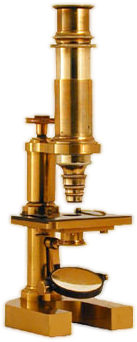
\includegraphics{images/IJ-icon-cover}%
 \end{minipage}
\begin{minipage}[c]{09.4cm}%
   \setlength{\tabcolsep}{0pt}
   \begin{tabular}{c} 
   \multicolumn{1}{l}{
       \textcolor{black!75}{\textbf{\Huge ImageJ User Guide}}}
   \tabularnewline[0.2cm]
   \hline 
   \noalign{\vskip6pt}
   \multicolumn{1}{r}{\textcolor{black!75}{\textbf{\LARGE \hfill{}IJ\,\theguideversion{}}}}
   \tabularnewline[0.7cm]
   \multicolumn{1}{c}{\textcolor{black!75}{\Large
     \href{mailto:tiago.ferreira@mail.mcgill.ca}{Tiago Ferreira}
     ~{$^{\footnotesize\bullet}$}~
     \href{mailto:wsr@nih.gov}{Wayne Rasband}}}
   \tabularnewline
   \end{tabular}
\end{minipage}\\
\vspace*{\fill}
\today
\par\end{center}
\vspace*{1cm}

%Frontnote
\begin{quote}
\hrulefill\qquad\textsc{Foreword}\qquad\hrulefill
\vspace*{\medskipamount}

The \emph{ImageJ User Guide} provides a detailed overview of ImageJ
(and inherently \nameref{sub:Fiji-intro}), the standard in scientific
image analysis.

It was thought as a comprehensive, fully-searchable, self-contained,
annotatable manual (\emph{see} \nameref{sec:Guide-Conventions}).
A \nomenclature{HTML}{HyperText Markup Language}HTML version is also
available as well as printer-friendly booklets (\emph{see} \nameref{sec:Guide-Formats}).
Its latest version can always be obtained from \url{http://imagej.nih.gov/ij/docs/guide}.
The source files are available through a Git version control repository
at \url{http://fiji.sc/guide.git}. 

\noindent Given ImageJ's heavy development this guide will always
remain incomplete. All ImageJ users and developers are encouraged
to contribute to the ImageJ documentation resources (\emph{see} \nameref{sub:Getting-Involved}).

\hrulefill
\end{quote}
%\vspace*{2.0cm}

\clearpage{}

\pagestyle{plain}

%TOC
 \pdfbookmark[1]{Contents}{tableofcontents}

\tableofcontents{}

\clearpage{}

\blfootnote{Please note that this is not an extensive list. Detailed release notes
for version\,\theguideversion{} are available on the ImageJ news
web site: \url{http://imagej.nih.gov/ij/notes.html}.}

\makelistofhighlights{Summarized Release Notes for ImageJ\,\theguideversion{}}\label{listoffeatures}

\clearpage{}

%Noteworthy
\phantomsection
\addcontentsline{toc}{section}{Noteworthy}
\phantomsection
\begin{doublespace}
\noindent

\listof{infobox}{Noteworthy}
\label{noteworthylist}

\end{doublespace}

\clearpage{}

%Listings
\phantomsection
\begin{doublespace}
\noindent

\makelistoflistings{Macro Listings}\label{macrolistingslist}

\end{doublespace}

\clearpage{}

\thispagestyle{empty}


\section*{Guide Formats\label{sec:Guide-Formats}}

This guide is available in the following formats:
\begin{lyxlist}{00.00.0000}
\item [{\textbf{Enhanced\ PDF}}] Optimized for electronic viewing and
highly enriched in hypertext links (\emph{see} \nameref{sec:Guide-Conventions}).
Available at \url{http://imagej.nih.gov/ij/docs/guide/user-guide.pdf}.
\item [{\textbf{HTML\ document}}] available online at \url{http://imagej.nih.gov/ij/docs/guide/}.
For offline usage a downloadable ZIP archive is also available at
\url{http://imagej.nih.gov/ij/docs/user-guide.zip}.
\item [{\textbf{Printable\ booklets}}] Two-sided booklets that can be
printed on a duplex unit printer by setting the automatic duplex mode
to ``short edge binding''. Two formats are available: A4 (\url{http://imagej.nih.gov/ij/docs/guide/user-guide-A4booklet.pdf})
and letter size paper (\url{http://imagej.nih.gov/ij/docs/guide/user-guide-USbooklet.pdf}).
\end{lyxlist}
\phantomsection
\addcontentsline{toc}{section}{Conventions}


\section*{Conventions Used in this Guide\label{sec:Guide-Conventions}}

\noindent Throughout the guide, internal  links are displayed in gray
(e.g., Part \prettyref{par:User-Interface1} \nameref{par:User-Interface1}).
Links to external URLs, such as the \href{http://imagej.nih.gov/ij/}{ImageJ website},
\url{http://imagej.nih.gov/ij/}, are displayed in dark blue.

\noindent ImageJ commands are typed in \textsf{sans\ serif} typeface
with respective shortcut keys flanked by square brackets (e.g.:\ \textsf{\userinterface{\noindent \textsf{Image\lyxarrow{}\nameref{sub:Duplicate...[D]}}}}).
As explained in \nameref{sub:Using-Shortcuts}, this notation implies
Shift-modifiers (i.e., \userinterface{\noindent {[}D{]}} means pressing
\mykeystroke{Shift} \mykeystroke{D}, \userinterface{\noindent {[}d{]}}
only the \mykeystroke{D} key) and assumes that \emph{Require control
key for shortcuts }in \textsf{\userinterface{\textsf{Edit\lyxarrow{}Options\lyxarrow{}\nameref{sub:Misc...}}}}
is unchecked. Note that references to the \mykeystroke{Ctrl} key
include the \mykeystroke{\cmd\  Cmd} key of Macintosh keyboards. 

\noindent Useful tips and reminders are placed in `Noteworthy notes'
numbered with upper case roman numerals (e.g., \ref{infobox:Frontmost-window}
\nameref{infobox:Frontmost-window}). The full list of these notes
is available \vpageref{noteworthylist}.

Filenames, directories and file extensions are typed in monospaced
font marked by a related icon, e.g., file \filenameref{StartupMacros.txt}
in folder \dirnameref{/Applications/ImageJ/macros/}.

\noindent Macro functions and code snippets are typed in monospaced
font, e.g., \texttt{\code{\noindent \texttt{resetMinAndMax()}}}.
Scripts and macros are numbered with arabic numerals included in parentheses
(e.g., \eqref{lis:RGBtoMGB1} \nameref{lis:RGBtoMGB1} \vpageref{lis:RGBtoMGB1})
and typeset with the same \index{Syntax highlighting}syntax markup
provided by the \nameref{sub:Fiji-Scrip-Editor}. The full list of
macro listings is available \vpageref{macrolistingslist}.

\noindent Selected highlights of version\,\theguideversion{} are
listed \vpageref{listoffeatures} and flagged with colored marginal
notes. These should be interpreted as:\medskip{}


\begin{minipage}[c][1\totalheight][t]{0.27\columnwidth}%
\qquad{}%
\begin{minipage}[c][1\totalheight][t]{2cm}%
\todo[inline,size=\footnotesize, backgroundcolor=green!20!white,bordercolor=green!60!white,nolist]{ 	\vspace*{-16pt}\begin{spacing}{0.8}\center\textsc{New in IJ\,\theguideversion}\end{spacing}\vspace*{1pt} }%
\end{minipage}%
\end{minipage}%
\begin{minipage}[c][1\totalheight][t]{0.73\columnwidth}%
\begin{singlespace}
\noindent {\small A new feature implemented in ImageJ\,\theguideversion{}.}\end{singlespace}
%
\end{minipage}\smallskip{}


\begin{minipage}[c][1\totalheight][t]{0.27\columnwidth}%
\qquad{}%
\begin{minipage}[c][1\totalheight][t]{2cm}%
\todo[inline,size=\footnotesize, backgroundcolor=yellow!20!white, bordercolor=yellow!60!white,nolist]{ 	\vspace*{-16pt}\begin{spacing}{0.8}\center\textsc{Improved in IJ\,\theguideversion}\end{spacing}\vspace*{1pt} }%
\end{minipage}%
\end{minipage}%
\begin{minipage}[c][1\totalheight][t]{0.73\columnwidth}%
\begin{singlespace}
\noindent {\small A routine that has been improved since previous
versions. Typically, a faster or more precise algorithm, a command
with better usability, or a task that has been extended to more image
types. }\end{singlespace}
%
\end{minipage}\smallskip{}


\begin{minipage}[c][1\totalheight][t]{0.27\columnwidth}%
\qquad{}%
\begin{minipage}[c][1\totalheight][t]{2cm}%
\todo[inline,size=\footnotesize, backgroundcolor=red!20!white, bordercolor=red!60!white,nolist]{ 	\vspace*{-16pt}\begin{spacing}{0.8}\center\textsc{Changed in IJ\,\theguideversion}\end{spacing}\vspace*{1pt} }%
\end{minipage}%
\end{minipage}%
\begin{minipage}[c][1\totalheight][t]{0.73\columnwidth}%
\begin{singlespace}
\noindent {\small A pre-existing command that has been renamed or
moved to a different menu location in ImageJ\,\theguideversion{}.}\end{singlespace}
%
\end{minipage}

\clearpage{}

\pagenumbering{arabic}
\pagestyle{fancy}
\thispagestyle{plain}


\part{Getting Started\label{part:Getting-Started}}

This part provides basic information on ImageJ installation, troubleshooting
and update strategies. It discusses \nameref{sub:Fiji-intro}\nomenclature{FIJI}{Fiji Is Just ImageJ}
and \nameref{sub:ImageJ2intro} as well as third-party software related
to ImageJ. Being impossible to document all the capabilities of ImageJ
without exploring technical aspects of image processing, external
resources allowing willing readers to know more about digital signal
processing are also provided.


\section{Introduction\label{sec:What-is-ImageJ?}}

ImageJ is a \href{http://rsb.info.nih.gov/ij/disclaimer.html}{public domain}
Java image processing and analysis program inspired by \href{http://rsb.info.nih.gov/nih-image/}{NIH Image}
for the Macintosh. It runs, either as an online applet or as a downloadable
application, on any computer with a Java\,1.5 or later virtual machine.
\href{http://imagej.nih.gov/ij/download.html}{Downloadable distributions}
are available for Windows, Mac OS\,X and Linux. It can display, edit,
analyze, process, save and print 8--bit, 16--bit and 32--bit images.
It can read many image formats including TIFF, GIF, JPEG, BMP, DICOM,
FITS and `raw'. It supports `stacks' (and hyperstacks), a series
of images that share a single window. It is multithreaded, so time-consuming
operations such as image file reading can be performed in parallel
with other operations%
\footnote{A somehow outdated list of ImageJ's features is available at \url{http://imagej.nih.gov/ij/features.html}%
}.

It can calculate area and pixel value statistics of user-defined selections.
It can measure distances and angles. It can create density histograms
and line profile plots. It supports standard image processing functions
such as contrast manipulation, sharpening, smoothing, edge detection
and median filtering.

It does geometric transformations such as scaling, rotation and flips.
Image can be zoomed up to 32\,:\,1 and down to 1\,:\,32. All analysis
and processing functions are available at any magnification factor.
The program supports any number of windows (images) simultaneously,
limited only by available memory.

Spatial calibration is available to provide real world dimensional
measurements in units such as millimeters. Density or gray scale calibration
is also available.

ImageJ was designed with an open architecture that provides extensibility
via Java plugins. Custom acquisition, analysis and processing plugins
can be developed using ImageJ's built in editor and Java compiler.
User-written plugins make it possible to solve almost any image processing
or analysis problem.

Being public domain open source software, an ImageJ user has the \href{http://wikieducator.org/The_right_license/The_essential_freedoms}{four essential freedoms}
defined by the Richard Stallman in 1986: 1) The freedom to run the
program, for any purpose; 2) The freedom to study how the program
works, and change it to make it do what you wish; 3) The freedom to
redistribute copies so you can help your neighbor; 4) The freedom
to improve the program, and release your improvements to the public,
so that the whole community benefits.

ImageJ is being developed on Mac OS\,X using its built in editor
and Java compiler, plus the \emph{BBEdit} editor and the \emph{Ant}
build tool. The source code is freely \href{http://imagej.nih.gov/ij/developer/source/index.html}{available}.
The author, Wayne Rasband (\href{mailto:wsr@nih.gov}{\nolinkurl{wsr@nih.gov}}),
is a Special Volunteer at the National Institute of Mental Health,
Bethesda, Maryland, USA.


\calso{\href{http://imagejdev.org/history}{History of ImageJ at imagejdev.org}}


\section{Installing and Maintaining ImageJ\label{sec:Updating-ImageJ}\index{Updates}}

ImageJ can be downloaded from \url{http://imagej.nih.gov/ij/download.html}.
Details on how to install ImageJ on \index{Linux}\href{http://imagej.nih.gov/ij/docs/install/linux.html}{Linux},
\href{http://imagej.nih.gov/ij/docs/install/mac.html}{Mac OS 9},
\index{Mac OS X}\href{http://imagej.nih.gov/ij/docs/install/osx.html}{Mac OS X}
and \index{Windows (OS)}\href{http://imagej.nih.gov/ij/docs/install/windows.html}{Windows}
\cite{C-WindowsInstaller} are available at \url{http://imagej.nih.gov/ij/docs/install/}
(\textsf{\userinterface{\textsf{Help\lyxarrow{}\nameref{sub:Installation...}}}}
command). Specially useful are the platform-specific \emph{Troubleshooting}
and \emph{Known Problems }sections. \index{Fiji}\nameref{sub:Fiji-intro}
installation is described at \url{http://fiji.sc/wiki/index.php/Downloads}.

The downloaded package may not contain the latest bug fixes so it
is recommended to upgrade ImageJ right after a first installation.
\index{Updates}Updating IJ\nomenclature{IJ}{ImageJ} consists only
of running \textsf{\userinterface{\textsf{Help\lyxarrow{}\nameref{sub:Update-ImageJ...}}}},
which will install the latest \filenameref{\href{http://imagej.nih.gov/ij/upgrade/}{ij.jar}}
in the ImageJ folder (on Linux and Windows) or inside the ImageJ.app
(on Mac OS\,X). 

\textsf{\userinterface{\textsf{Help\lyxarrow{}\nameref{sub:Update-ImageJ...}}}}
can be used to upgrade (or downgrade) the \filenameref{ij.jar} file
to \emph{release updates} or \emph{daily builds}. Release updates
are announced frequently on the \href{http://imagej.nih.gov/ij/notes.html}{IJ news website}
and are labelled alphabetically (e.g., v.\,1.43m). Typically, these
releases contain several new features and bug fixes, described in
detail on the \href{http://imagej.nih.gov/ij/notes.html}{ImageJ News page}.
\emph{Daily builds,} on the other hand, are labelled with numeric
sub-indexes (e.g., v.\,1.43n4) and are often released without documentation.
Nevertheless, if available, release notes for daily builds can be
found at \url{http://imagej.nih.gov/ij/source/release-notes.html}.
When a release cycle ends (v.\,1.42 ended with 1.42q, v.\,1.43 with
1.43u, etc.) an \emph{installation package }is created, downloadable
from \url{http://imagej.nih.gov/ij/download.html}. Typically, this
package is bundled with a small list of add-ons (\nameref{sub:Macros-ExtendingIJ},
\nameref{sub:Scripts} and \nameref{sub:Plugins}).


\calso{\href{http://imagej.nih.gov/ij/macros/toolsets/Luts\%20Macros\%20and\%20Tools\%20Updater.txt}{Luts, Macros and Tools Updater},
a macro toolset that performs live-updating of \href{http://imagej.nih.gov/ij/macros/}{macros}
listed on the ImageJ web site}


\subsection{ImageJDistributions\label{sec:ImageJ-Distributions}}

ImageJ alone is not that powerful: it's real strength is the vast
repertoire of \nameref{sub:Plugins} that extend ImageJ's functionality
beyond its basic core. The many hundreds, probably thousands,  freely
available plugins from contributors around the world play a pivotal
role in ImageJ's success \cite{Collins:2007p13684}. Running \textsf{\userinterface{\textsf{Help\lyxarrow{}\nameref{sub:Update-ImageJ...}}}},
however, will not update any of the plugins you may have installed%
\footnote{Certain plugins, however, provide self-updating mechanisms (e.g.,
\href{http://simon.bio.uva.nl/objectj/}{ObjectJ} and the \index{Bio-Formats}\href{http://loci.wisc.edu/software/bio-formats}{OME Bio-Formats}).%
}.

ImageJ add-ons (\nameref{sub:Plugins}, \nameref{sub:Scripts} and
\nameref{sub:Macros-ExtendingIJ}) are available from several sources
(\href{http://imagej.nih.gov/ij/plugins/}{ImageJ's plugins page}
{[}\textsf{\userinterface{\textsf{Help\lyxarrow{}\nameref{sub:Plugins...}}}}{]},
\href{http://imagejdocu.tudor.lu/doku.php?id=plugin:start}{ImageJ Information and Documentation Portal}
and \href{http://fiji.sc/wiki/index.php/Category:Plugins}{Fiji's webpage},
among others) making manual updates of a daunting task. This reason
alone, makes it extremely convenient the use of \nameref{sec:ImageJ-Distributions}
bundled with a pre-organized collection of add-ons.

Below is a list of the most relevant projects that address the seeming
difficult task of organizing and maintaining ImageJ beyond its basics.
If you are a life scientist and have doubts about which distribution
to choose you should opt for \nameref{sub:Fiji-intro}. It is heavily
maintained, offers an automatic updater, improved scripting capabilities
and ships with powerful plugins. More specialized adaptations of ImageJ
are discussed in \nameref{sub:Other-Software-Packages}.


\subsubsection*{Fiji\label{sub:Fiji-intro}}

\href{http://fiji.sc/}{Fiji}\index{Fiji} (\emph{Fiji Is Just ImageJ---Batteries
included}) is a distribution of ImageJ together with Java, Java 3D
and several plugins organized into a coherent menu structure. Citing
its developers, ``Fiji compares to ImageJ as Ubuntu compares to Linux''.
The main focus of Fiji is to assist research in life sciences, targeting
image registration, stitching, segmentation, feature extraction and
3D visualization, among others. It also supports many scripting languages
(BeanScript, Clojure, Jython, Python, Ruby, \emph{see} \nameref{sec:ScriptingOtherLang}).
Importantly, Fiji ships with a \href{http://fiji.sc/wiki/index.php/Update_Fiji}{convenient updater}
that knows whether your files are up-to-date, obsolete or locally
modified. \href{http://fiji.sc/wiki/index.php/Documentation}{Comprehensive documentation}
is available for most of its plugins. The Fiji project was presented
publicly for the first time at the \href{http://imagejconf.tudor.lu/doku.php}{ImageJ User and Developer Conference}
in November 2008.


\subsubsection*{MBF\ ImageJ\label{sub:MBFImageJintro}}

The \index{MBF ImageJ}\index{ImageJ for Microscopy@ImageJ for Microscopy  \see{MBF ImageJ,}}\href{http://www.macbiophotonics.ca/imagej/}{MBF ImageJ bundle}
or \emph{ImageJ for Microscopy} (formerly \href{http://www.uhnres.utoronto.ca/facilities/wcif/imagej/}{WCIF-ImageJ})
features a collection of plugins and macros, collated and organized
by Tony Collins at the MacBiophotonics facility, McMaster University.
It is accompanied by a \href{http://www.macbiophotonics.ca/imagej/}{comprehensive manual}
describing how to use the bundle with light microscopy image data.
It is a great resource for microscopists but is not maintained actively,
lagging behind the development of core ImageJ.

Note that you can add plugins from MBF ImageJ to Fiji, combining the
best of both programs. Actually, you can use multiple ImageJ distributions
simultaneously, assemble your own ImageJ bundle by gathering the plugins
that best serve your needs (probably, someone else at your institution
already started one?) or create symbolic links to share plugins between
different installations.


\calso{Description of all ImageJ related projects at \href{http://imagejdev.org/faq\#n141}{ImageDev}}


\subsection{Related Software\label{sub:Related-Software}}


\subsubsection{Software Packages Built on Top of ImageJ\label{sub:Other-Software-Packages}}
\begin{description}
\item [{Bio7}] \href{http://bio7.org/}{Bio7} is an integrated development
environment for \index{Bio7}ecological modeling with a main focus
on individual based modeling and spatially explicit models. Bio7 features:
Statistical analysis (using R); Spatial statistics; Fast communication
between \index{R (GNU S)@R (GNU S)  \see{Interoperability,}}R and
Java; BeanShell and Groovy support; Sensitivity analysis with an embedded
flowchart editor and creation of 3D OpenGL (Jogl) models (\emph{see
also} RImageJ in \nameref{sec:ImageJ-Interoperability}).
\item [{BoneJ}] \href{http://bonej.org/}{BoneJ} \index{BoneJ}is a collection
of tools for trabecular geometry and whole bone shape analysis.
\item [{$\micro$Manager}] \href{http://www.micro-manager.org/}{Micro-Manager}
is a software package for control of automated microscopes. It lets
you execute common microscope image acquisition strategies such as
time-lapses, multi-channel imaging, z-stacks, and combinations thereof.
\index{Micro@$\micro$Manager}$\micro$Manager works with microscopes
from all four major manufacturers, most scientific-grade cameras and
many peripherals used in microscope imaging.
\item [{MRI--CIA}] \href{http://www.mri.cnrs.fr/index.php?m=38}{MRI Cell Image Analyzer},
developed by the Montpellier RIO Imaging facility (CNRS), is a rapid
image analysis application development framework, adding visual scripting
interface to ImageJ's capabilities. It can create batch applications
as well as interactive applications. The applications include the
topics \textquotedblleft{}DNA combing\textquotedblright{}, \textquotedblleft{}quantification
of stained proteins in cells\textquotedblright{}, \textquotedblleft{}comparison
of intensity ratios between nuclei and cytoplasm\textquotedblright{}
and \textquotedblleft{}counting nuclei stained in different channels''.
\item [{ObjectJ}] \href{http://simon.bio.uva.nl/objectj/index.html}{ObjectJ},
the successor of \href{http://simon.bio.uva.nl/Object-Image/object-image.html}{object-image},
supports graphical vector objects that non-destructively mark images
on a transparent layer. Vector objects can be placed manually or by
macro commands. Composite objects can encapsulate different color-coded
marker structures in order to bundle features that belong together.
ObjectJ provides back-and-forth navigation between results and images.
The results table supports statistics, sorting, color coding, qualifying
and macro access.
\item [{SalsaJ}] \href{http://www.euhou.net/index.php?option=com_content&task=view&id=7&Itemid=9}{SalsaJ}
is a student-friendly software developed specifically for the \href{http://www.euhou.net/}{EU-HOU project}.
It is dedicated to image handling and analysis of astronomical images
in the classroom. \index{SalsaJ}SalsaJ has been translated into several
languages.
\item [{\label{misc:TrakEM2}TrakEM2}] \href{http://www.ini.uzh.ch/~acardona/trakem2.html}{TrakEM2}
is a program for morphological \index{Data mining@Data mining \see{TrakEM2,}}data
mining, three-dimensional \index{Modeling@Modeling \see{TrakEM2 and Bio7,}}modeling
and image stitching, registration, editing and annotation \cite{Cardona:2010p18306}.
\index{TrakEM2}\index{Fiji}TrakEM2 is \href{http://fiji.sc/wiki/index.php/TrakEM2}{distributed with Fiji}
and \href{http://www.ini.uzh.ch/~acardona/trakem2_manual.html}{capable of}:\vspace{-8pt}


\begin{description}
\item [{3D\ modeling}] Objects in 3D, defined by sequences of contours,
or profiles, from which a skin, or mesh, can be constructed, and visualized
in 3D.
\item [{Relational\ modeling}] The extraction of the map that describes
links between objects. For example, which neuron contacts which other
neurons through how many and which synapses. 
\end{description}
\end{description}

\calso{\index{BioImageXD}\href{http://www.bioimagexd.net/}{BioImageXD},
\index{Endrov}\href{http://www.endrov.net/}{Endrov}, \index{Image SXM}\href{http://www.liv.ac.uk/\%7Esdb/ImageSXM/}{Image SXM}}


\subsubsection{ImageJ Interoperability\label{sec:ImageJ-Interoperability}}

Several packages exist that allow ImageJ to \index{Interoperability}interact
with other applications/environments:
\begin{description}
\item [{Bitplane\ Imaris}] \href{http://www.bitplane.com/go/products/imarisxt}{ImarisXT}
can load and execute ImageJ plugins. \index{Imaris}\href{http://www.bitplane.com/go/products/imarisxt/xtensions/imagej}{bpImarisAdapter}
(Windows only and requiring valid licenses for Imaris and ImarisXT)
allows the exchange of images between Imaris and ImageJ.
\item [{CellProfiler}] \index{CellProfiler@CellProfiler  \see{Interoperability,}}\href{http://www.cellprofiler.org/}{CellProfiler}
\cite{Carpenter:2006p1986} features \href{http://cellprofiler.org/CPmanual/RunImageJ.html}{RunImageJ},
a module that allows ImageJ plugins to be run in a CellProfiler pipeline.
\item [{Icy}] \href{http://www.bioimageanalysis.org/icy/}{Icy}, an open
source community software for \index{Icy}bio-imaging, executes ImageJ
plugins with almost 100\% plugin compatibility. 
\item [{Knime}] \index{Knime} \href{http://knime.org/}{Knime} (\nomenclature{Knime}{Konstanz Information Miner}Konstanz
Information Miner) contains several image processing nodes (\nomenclature{KNIP}{Knime Image Processing}\href{http://tech.knime.org/community/image-processing}{KNIP}\index{KNIP@KNIP  \see{Knime,}})
that are capable of executing ImageJ plugins and macros.
\item [{Open\ Microscopy\ Environment}] \nomenclature{OME}{Open Microsopy Environment}All
\href{http://www.openmicroscopy.org/}{Open Microscopy Environment}
projects such as \index{Bio-Formats}\href{http://www.openmicroscopy.org/site/products/bio-formats}{Bio-Formats},
\href{http://www.openmicroscopy.org/site/products/visbio}{VisBio}
and \href{http://www.openmicroscopy.org/site/products/omero}{OMERO}
integrate well with ImageJ.
\item [{RImageJ\ ---\ R\ bindings\ for\ ImageJ}] Bindings between
ImageJ and \index{R (GNU S)@R (GNU S)  \see{Interoperability,}}\href{http://www.r-project.org/}{R (GNU S)}
--- The free software environment for statistical computing and graphics.
The documentation for RImageJ is available at \url{http://cran.r-project.org/web/packages/RImageJ/RImageJ.pdf}
(\emph{see also} Bio7 in \nameref{sub:Other-Software-Packages}).
\item [{MIJ\ ---\ Matlab--ImageJ\ bi-directional\ communication}] A
Java package for bi-directional data exchange between \index{MATLAB@MATLAB  \see{Interoperability,}}Matlab
and ImageJ, allowing to exchange images between the two imaging software.
\index{MIJ@MIJ  \see{Interoperability,}}MIJ also allows MATLAB to
access all built-in functions of ImageJ as well as third-party ImageJ
plugins. The developers provide more information on the \href{http://bigwww.epfl.ch/sage/soft/mij/}{MIJ}
and \href{http://www.mathworks.com/matlabcentral/fileexchange/32344-hardware-accelerated-3d-viewer-for-matlab}{Matlab File Exchange}
websites. \nameref{sub:Fiji-intro} features \code{\href{http://fiji.sc/wiki/index.php/Miji}{Miji.m}},
which makes even more convenient to use the libraries and functions
provided by Fiji's components from within Matlab.
\end{description}

\calso{\href{http://imagej.nih.gov/ij/links.html}{ImageJ related links},
list of \href{http://developer.imagej.net/category/web-links/related-imaging-software}{related imaging software}
on the \nameref{sub:ImageJ2intro} website}


\subsection{ImageJ2\label{sub:ImageJ2intro}}

\href{http://imagejdev.org/}{ImageJDev} is a \href{http://imagejdev.org/funding}{federally funded},
\href{http://imagejdev.org/collaborators}{multi-institution} project
dedicated to the development of the next-generation version of ImageJ:
``\index{ImageJ2}ImageJ2''. \index{ImageJ2}\index{ImageDev@ImageDev \see{ImageJ2,}}ImageJ2
is a complete rewrite of ImageJ, that includes the current, stable
version ImageJ (``ImageJ1'') with a compatibility layer so that
old-style plugins and macros can run the same as they currently do
in ImageJ1. Below is a \href{http://imagejdev.org/aims}{summary}
of the \href{http://imagejdev.org/}{ImageJDev} project aims: 
\begin{itemize}
\item To create the next generation version of ImageJ and improve its core
architecture based on the needs of the community.
\item To ensure ImageJ remains useful and relevant to the broadest possible
community, maintaining backwards compatibility with ImageJ1 as close
to 100\% as possible.
\item Expand functionality by interfacing ImageJ with existing open-source
programs.
\item To lead ImageJ development with a clear vision, avoiding duplication
of efforts
\item To provide a central online resource for ImageJ: program downloads,
a plugin repository, developer resources and more.
\end{itemize}
Be sure to follow the ImageJ2 \href{http://imagejdev.org/recent_changes}{project news}
and the \href{http://imagejdev.org/blog}{ImageDev blog} for updates
on this exciting project.


\section{Getting Help\label{sec:Help-Resources}\index{Help resources}}


\subsection{Help on Image Analysis}

\index{Ethics@Ethics \see{Acceptable manipulation,}}\index{Acceptable manipulation}Below
is a list of online resources (in no particular order) related to
image processing and scientific image analysis, complementing the
list of \href{http://imagej.nih.gov/ij/links.html}{external resources on the IJ web site}. 


\subsubsection*{Ethics in Scientific Image Processing}
\begin{itemize}
\item \href{http://www.ori.dhhs.gov/education/products/RIandImages/default.html}{Online learning Tool for Research Integrity and Image Processing}\\
This website, created by the \href{http://ori.dhhs.gov/}{Office of Research Integrity},
explains what is appropriate in image processing in science and what
is not.
\item \href{http://swehsc.pharmacy.arizona.edu/exppath/micro/digimage_ethics.php}{Digital Imaging: Ethics (at the Cellular Imaging Facily Core, SEHSC)}\\
This website, compiled by Douglas Cromey at the University of Alabama
-- Birmingham, discusses thoroughly the topic of digital imaging ethics.
It is recommended for all scientists. The website contains links to
several external resources, including:\vspace{-8pt}


\begin{enumerate}
\item \href{http://www.jcb.org/cgi/reprint/166/1/11}{What's in a picture? The temptation of image manipulation}
(2004) M Rossner and K M Yamada, J Cell Biology 166(1):11--15, doi:10.1083/jcb.200406019
\item \href{http://www.nature.com/nature/journal/v439/n7079/full/439891b.html}{Not picture-perfect}
(2006), Nature 439, 891--892, doi:10.1038/439891b.
\end{enumerate}
\end{itemize}

\subsubsection*{Scientific Image Processing\index{Image processing (help)}\label{sub:IP-Resources}}
\begin{itemize}
\item \href{http://fiji.sc/wiki/index.php/IP_Principles}{What you need to know about scientific image processing}\\
Simple and clear, this \nameref{sub:Fiji-intro} webpage explains
basic aspects of scientific image processing.
\item \href{http://www.imagingbook.com}{imagingbook.com}\\
Web site of \emph{Digital Image Processing: An Algorithmic Introduction
using Java} by Wilhelm Burger and Mark Burge \cite{Burger:2008p14082}.
This technical book provides a modern, self-contained, introduction
to digital image processing techniques. Numerous complete Java implementations
are provided, all of which work within ImageJ.
\item \href{http://homepages.inf.ed.ac.uk/rbf/HIPR2/}{Hypermedia Image Processing Reference (HIPR2)}\\
Developed at the Department of Artificial Intelligence in the University
of Edinburgh, provides on-line reference and tutorial information
on a wide range of image processing operations.
\item \href{https://ifn.mpi-cbg.de/wiki/ifn/index.php/Imaging_Facility_Network}{IFN wikipage}\\
The Imaging Facility Network (IFN) in Biopolis Dresden provides access
to advanced microscopy systems and image processing. The website hosts
high quality \href{https://ifn.mpi-cbg.de/wiki/ifn/index.php/Teaching_Material}{teaching material}
and useful links to external resources.
\item \href{http://www.stereology.info/}{stereology.info} \\
Stereology Information for the Biological Sciences, designed to introduce
both basic and advanced concepts in the field of stereology.
\end{itemize}

\calso{ImageJ Related Publications on page \pageref{sec:IJ-related-pub}}


\subsection{Help on ImageJ\label{sub:Getting-Help}}

Below is a list of the ImageJ \index{Help resources}help resources
that complement this guide (\emph{see} \nameref{sec:Guide-Formats}).
Specific documentation on advanced uses of ImageJ (macro programming,
plugin development, etc.) is discussed in \nameref{sec:Extending-ImageJ}.
\begin{enumerate}
\item The ImageJ \href{http://imagej.nih.gov/ij/docs/}{online documentation pages}\\
Can be accessed via the \textsf{\userinterface{\textsf{Help\lyxarrow{}\nameref{sub:Documentation...}}}}
command.
\item The \index{Fiji}\nameref{sub:Fiji-intro} webpage:\\
\url{http://fiji.sc/}
\item The ImageJ Information and Documentation Portal (ImageJ wikipage):\\
\href{http://imagejdocu.tudor.lu/doku.php}{http://imagejdocu.tudor.lu/doku.php}
\item Video \index{Tutorials}tutorials on the ImageJ Documentation Portal
and the Fiji YouTube channel:\\
\url{http://imagejdocu.tudor.lu/doku.php?id=video:start&s[]=video}
and \url{http://www.youtube.com/user/fijichannel}. New ImageJ users
will probably profit from \href{http://imagejdocu.tudor.lu/doku.php?id=video:beginner_help:imagej_beginner_s_tutorial}{Christine Labno's video tutorial}.
\item The \index{MBF ImageJ}ImageJ for Microscopy manual\\
\url{http://www.macbiophotonics.ca/imagej/}
\item Several online documents, most of them listed at:\\
\url{http://imagej.nih.gov/ij/links.html} and \url{http://imagej.nih.gov/ij/docs/examples/}
\item Mailing lists:\index{Mailing lists@Mailing lists \see{Help resources,}}

\begin{enumerate}
\item \textbf{ImageJ} --- \url{http://imagej.nih.gov/ij/list.html}\\
General user and developer discussion about ImageJ. Can be accessed
via the \textsf{\userinterface{\textsf{Help\lyxarrow{}\nameref{sub:List-Archives...}}}}
command. This list is also mirrored at \href{http://imagej.1557.n6.nabble.com/}{Nabble}
and \href{http://dir.gmane.org/gmane.comp.java.imagej}{Gmane}. You
may find it easier to search and browse the list archives on these
mirrors. Specially useful are the \href{feed://rss.gmane.org/topics/excerpts/gmane.comp.java.imagej}{RSS feeds}
and the\emph{ \href{http://news.gmane.org/gmane.comp.java.imagej}{frames and threads}}
view provided by Gmane.
\item \textbf{Fiji users }--- \url{http://groups.google.com/group/fiji-users}\\
For user discussion specific to \nameref{sub:Fiji-intro} (rather
than core ImageJ).
\item \textbf{Fiji-devel} --- \url{http://groups.google.com/group/fiji-devel}\\
For developer discussion specific to Fiji.
\item \textbf{ImageJ-devel} --- \url{http://imagejdev.org/mailman/listinfo/imagej-devel}\\
For communication and coordination of the ImageJDev project.
\item \textbf{Dedicated mailing lists} for ImageJ related projects\\
Described at \url{http://imagejdev.org/mailing-lists} .
\end{enumerate}
\end{enumerate}

\subsubsection*{Using Mailing-lists}

If you are having problems with ImageJ, you should inquiry about them
in the appropriated \index{Help resources}list. The ImageJ mailing
list is an unmoderated forum subscribed by a knowledgeable worldwide
user community with $\thickapprox$2000 advanced users and developers.
To have your questions promptly answered you should consider the following:
\begin{enumerate}
\item Read the documentation files (described earlier in this section) before
posting. Because there will always be a natural lag between the implementation
of key features and their documentation it may be wise to check briefly
the ImageJ news website (\textsf{\userinterface{\textsf{Help\lyxarrow{}\nameref{sub:ImageJ-News...}}}}).
\item Look up the mailing list archives (\textsf{\userinterface{\textsf{Help\lyxarrow{}\nameref{sub:List-Archives...}}}}).
Most of your questions may have already been answered.
\item If you think you are facing a \index{Bug (reporting)@Bug (reporting) \seealso{Debug,}}bug
try to upgrade to the latest version of ImageJ (\textsf{\userinterface{\textsf{Help\lyxarrow{}\nameref{sub:Update-ImageJ...}}}}).
You should also check if you are running the latest version of the
Java Virtual Machine for your operating system. Detailed instructions
on how to submit a bug report are found at \url{http://imagej.nih.gov/ij/docs/faqs.html#bug}.
\item Remember that in most cases you can find answers within your own ImageJ
installation without even connecting to the internet since the heuristics
for finding commands or writing macros have been significantly improved
in later versions (\emph{see} \nameref{sec:Finding-Commands} and
\nameref{sec:Extending-ImageJ}).
\item As with any other mailing list, you should always follow basic \href{http://en.wikipedia.org/wiki/Netiquette}{netiquette},
namely:

\begin{enumerate}
\item Use descriptive subject lines -- \emph{Re: Problem with Image>Set
Scale command }is much more effective than a general\emph{ Re: Problem.}
\item Stay on topic -- Do not post off-topic messages, unrelated to the
message thread.
\item Be careful when sending attachments -- Refrain from attaching large
files. Use, e.g., a \href{http://en.wikipedia.org/wiki/File_hosting_service\#Comparison_of_notable_file_hosting_services}{file hosting service}
instead.
\item Edit replies -- You should include only the minimum content that is
necessary to provide a logical flow from the question to the answer,
i.e., quote only as much as absolutely necessary and relevant.\end{enumerate}
\end{enumerate}



\clearpage{}

\thispagestyle{plain}


\part{Working with ImageJ\label{part:Working-with-ImageJ}}

This part introduces some basic aspects of ImageJ so that you can
use the software more efficiently. It also introduces some important
terms and concepts used throughout this guide. You may skip it if
you already use the program efficiently and are familiar with terms
such as \nameref{sub:Virtual-Stacks}, \nameref{sub:Hyperstacks-Intro},
\nameref{sub:Pseudocolor-Images}, \nameref{sub:Color-Composites}
or \nameref{sub:Composite-selections}.


\section{Using Keyboard Shortcuts\label{sub:Using-Shortcuts}}

You'll learn more and more \index{Keyboard@Keyboard \see{Shortcuts and Modifier keys,}}\index{Shortcuts}shortcut
keys as you use ImageJ, because (almost) all shortcuts are listed
throughout ImageJ menus. Similarly, in this guide each command has
its shortcut key listed on its name (flanked by square brackets).
Please note that the notation for these key-bindings is case sensitive,
i.e., Shift-modifiers are not explicitly mentioned (a capital \textsf{A}
means \textsf{Shift--A}) and assumes that \emph{Require control key
for shortcuts }in \textsf{\userinterface{\textsf{Edit\lyxarrow{}Options\lyxarrow{}\nameref{sub:Misc...}}}}
is unchecked (i.e., except when using the IJ \nameref{sub:ImageJ-Macro-Editor}
or the \nameref{sec:Text-Tool}, you won't have to hold down the Control
key to use menu shortcuts). For example, the command \textsf{\userinterface{\textsf{Edit\lyxarrow{}\nameref{sub:Invert-[I]}}}}
can be evoked by \mykeystroke{Shift} \mykeystroke{I} or \mykeystroke{Ctrl}
\mykeystroke{Shift} \mykeystroke{I} if \emph{Require control key
for shortcuts }is checked. The full list of ImageJ shortcuts (\emph{see}
\nameref{sec:Keyboard-Shortcuts}) can be retrieved at any time using
the \textsf{\userinterface{\textsf{Plugins\lyxarrow{}Utilities\lyxarrow{}\nameref{sub:List-Shortcuts...}}}}
command.

There are three \index{Modifier keys}modifier keys in ImageJ:
\begin{lyxlist}{00.00.0000}
\item [{\textbf{Control}}] (\textbf{Command Key}\index{Command key} on
Apple keyboards) Denoted by `Ctrl'\nomenclature{Ctrl}{Control key. In this guide also the Command key in Apple keyboards}
or \mykeystroke{Ctrl} in this document. Although a control key is
typically present on Apple keyboards, on a Macintosh computer running
ImageJ the Command key \mykeystroke{\cmd\  Cmd} replaces the functionality
of the Control key of other operating systems. For sake of simplification,
`Ctrl' will always refer to both  throughout this guide.
\item [{\textbf{Shift}}] Denoted by `Shift'\nomenclature{Shift}{Shift key}
or \mykeystroke{Shift} in this document.
\item [{\textbf{Alt}}] Denoted by `Alt'\nomenclature{Alt}{Alt, Option or Meta key}
or \mykeystroke{Alt} in this document. This is also the `Option'
or `Meta' key on many keyboards. In ImageJ, it is also used to type
special unit symbols such as $\micro$ (\mykeystroke{Alt}\mykeystroke{M})
or $\angstrom$ (\mykeystroke{Alt}\mykeystroke{Shift}\mykeystroke{A}). 
\end{lyxlist}

\calso{\nameref{sec:Keyboard-Shortcuts}, \userinterface{Plugins\lyxarrow{}\nameref{sub:Shortcuts}}}

\begin{infobox}
\caption{\label{infobox:Frontmost-window}Frontmost Window and Window Activation}


\noindent In ImageJ, all operations are performed on the active (frontmost)
image (which has its title bar highlighted). If a window is already
open it will activate when its opening command is re-run, e.g., if
the B\&C window is already opened (\userinterface{\noindent Image\lyxarrow{}Adjust\lyxarrow{}\nameref{sub:Brightness/Contrast...[C]}}),
pressing its keyboard shortcut (\,\mykeystroke{\noindent Shift}
\mykeystroke{C}\,) will activate it. \medskip{}


\noindent Pressing \mykeystroke{\noindent Enter} on any image will
bring the \nameref{fig:The-ImageJ-window} to the foreground. In addition,
it is also possible to permanently place the main window above all
other windows (\emph{see}  \nameref{sub:FloatingMainWin}).
\end{infobox}



\section{Finding Commands\label{sec:Finding-Commands}}

Navigating through the extensive list of ImageJ commands, macros and
plugins may be quite cumbersome. Through its built-in Command Finder\,/\,Launcher\cite{C-ComandFinder},
ImageJ offers an expedite alternative that allows you to retrieve
commands extremely fast: \textsf{\userinterface{\textsf{Plugins\lyxarrow{}Utilities\lyxarrow{}\nameref{sub:Command-Finder}}}}.

In addition, ImageJ features a find function that locates macros,
scripts and plugins source (\filenameref{.java}) files on your computer:
the \textsf{\userinterface{\textsf{Plugins\lyxarrow{}Utilities\lyxarrow{}\nameref{sub:Search...}}}}
command. Because most of IJ source files contain circumstanced comments,
you can use this utility to retrieve files related not only to a image
processing routine (e.g.,\emph{ background }or\emph{ co-localization})
but also to a practical context such as \emph{radiogram}, \emph{cell}
or \emph{histology}. Indeed, ImageJ source files contain detailed
annotations useful to both developers and regular users that want
to know more about ImageJ routines and algorithms.

\textsf{\userinterface{\textsf{\nameref{sub:Search...}}}} and \textsf{\userinterface{\textsf{\nameref{sub:Command-Finder}}}}
are described in detail in \textsf{\userinterface{\textsf{Plugins\lyxarrow{}\nameref{sub:Utilities}}}}.
\begin{figure}
\noindent \begin{centering}
\hspace{11.1em}\textsf{\small Plugins\lyxarrow{}Utilities\lyxarrow{}\nameref{sub:Command-Finder}\vspace{3pt}
}
\par\end{centering}{\small \par}

\noindent \begin{centering}
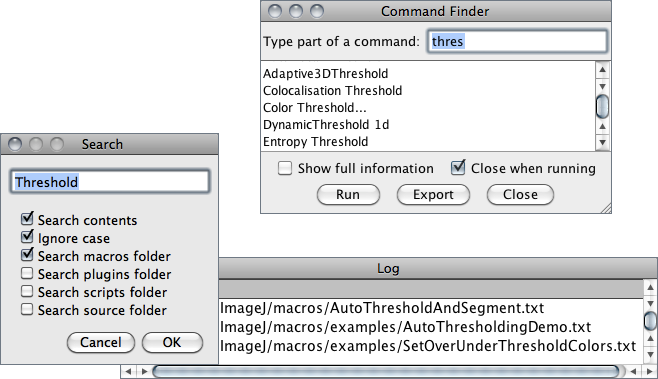
\includegraphics[scale=0.55]{images/CommandFinderAndSearch}
\par\end{centering}

\noindent \centering{}\textsf{\small Plugins\lyxarrow{}Utilities\lyxarrow{}\nameref{sub:Search...}}
\end{figure}



\calso{\nameref{sub:Control-Panel...}, \nameref{sec:Keyboard-Shortcuts}
and \filenameref{\href{http://imagej.nih.gov/ij/macros/SourceCodeRetriever.txt}{SourceCodeRetriever}},
a macro that searches for a menu entry and retrieves the source file
of the respective command}


\section[Undo and Redo]{Undo and Redo\label{sec:Undo-and-Redo}}

Probably the first thing you will notice is that ImageJ does not have
a large \index{Undo}undo/redo buffer. Undo (\textsf{\userinterface{\textsf{Edit\lyxarrow{}\nameref{sub:Undo-[z]}}}})
is currently limited to the most recent image editing\,/\,filtering
operation. With time you will appreciate that this is necessary to
minimize memory overhead. Nevertheless, with IJ\,1.45 and later,
\textsf{\userinterface{\textsf{\nameref{sub:Undo-[z]}}}} is, in most
cases, undoable and can be applied to multiple images if \emph{Keep
multiple undo buffers }is checked in \textsf{\userinterface{\textsf{Edit\lyxarrow{}Options\lyxarrow{}\nameref{sub:Memory-&-Threads...}}}}

If you cannot recover from a mistake, you can always use \textsf{\userinterface{\textsf{File\lyxarrow{}\nameref{sub:Revert[r]}}}}
to reset the image lo its last saved state. For selections, \textsf{\userinterface{\textsf{Edit\lyxarrow{}Selection\lyxarrow{}\nameref{sub:Restore-Selection-[E]}}}}
can be used to recover any misdealt selection.

In ImageJ the equivalent to \index{Redo}`Redo' is the \textsf{\userinterface{\textsf{Process\lyxarrow{}\nameref{sub:Repeat-Command-[R]}}}},
that re-runs the previous used command (skipping \textsf{\userinterface{\textsf{Edit\lyxarrow{}\nameref{sub:Undo-[z]}}}}
and \textsf{\userinterface{\textsf{File\lyxarrow{}\nameref{sub:Open...}}}}
commands).


\calso{\textsf{\userinterface{\textsf{Plugins\lyxarrow{}Utilities\lyxarrow{}\nameref{sub:Reset...}}}},
\href{http://imagejdocu.tudor.lu/doku.php?id=plugin:utilities:multi_undo:start}{Multi Undo}
plugin}


\section{Image Types and Formats\label{sec:Image-Types}}

\index{Image types}Digital Images are two-dimensional grids of pixel\nomenclature{pixel}{Picture element}
intensities values with the width and height of the image being defined
by the number of pixels in $x$ (rows) and $y$ (columns) direction.
Thus, pixels (picture elements) are the smallest single components
of images, holding numeric values -- pixel intensities -- that range
between black and white. The characteristics of this range, i.e.,
the number of unique intensity (brightness) values that can exist
in the image is defined as the bit\nomenclature{bit}{Binary digit}--depth
of the image and specifies the level of precision in which intensities
are coded, e.g.: A 2--bit image has $2^{2}=4$\,tones: 00 (black),
01 (gray), 10 (gray), and 11 (white). A 4--bit image has $2^{4}=16$\,tones
ranging from 0000 (0) to 1111 (16), etc. In terms of bits per pixel
(bpp\nomenclature{bpp}{Bits per pixel}), the most frequent types
of images (\userinterface{Image\lyxarrow{}\nameref{sub:Type}}) that
ImageJ deals with are (\index{ImageJ2}\nameref{sub:ImageJ2intro}
supports \href{http://imagejdev.org/imagej2-pixel-types}{many more types of image data}):
\begin{lyxlist}{RGB-Color---}
\item [{\textbf{8--bit}}] \noindent Images that can display 256 ($2^{8}$)
gray levels (integers only).
\item [{\textbf{16--bit}}] \noindent Images that can display 65,\,536
($2^{16}$) gray levels (integers only).
\item [{\textbf{32--bit}}] \noindent Images that can display 4,\,294,\,967,\,296
($2^{32}$) gray levels (real numbers). In 32--bit images, pixels
are described by \href{http://en.wikipedia.org/wiki/Floating_point}{floating point}
values and can have\textsc{ any} intensity value including \emph{NaN}\nomenclature{NaN}{Not a Number}
(Not a Number).
\item [{\textbf{RGB\ Color}}] \noindent \nameref{sec:Color-Images} that
can display 256 values in the \uline{R}ed, \uline{G}reen and
\uline{B}lue channel. These are 24--bit ($2^{3\times8}$) images.
RGB\nomenclature{RGB}{Red Green Blue} color images can also be 32--bit
color images (24--bit color images with additional eight bits coding
alpha blending values, i.e., transparency).
\end{lyxlist}

\subsection*{Native Formats\label{sub:Native-Formats}}

Natively (i.e.\ without the need of third-party plugins) ImageJ opens
the following formats: \textbf{TIFF}\nomenclature{TIFF}{Tagged Image File Format},
\textbf{GIF}\nomenclature{GIF}{Graphics Interchange Format}, \textbf{JPEG}\nomenclature{JPEG}{Joint Photographic Experts Group},
\textbf{PNG}\nomenclature{PNG}{Portable Network Graphics}, \textbf{DICOM}\nomenclature{DICOM}{Digital Imaging and Communications in Medicine},
\textbf{BMP}\nomenclature{BMP}{Bitmap Image File (Device Independent Bitmap, DIB)},
\textbf{PGM}\nomenclature{PGM}{Portable GrayMap} and \textbf{FITS}\nomenclature{FITS}{Flexible Image Transport System}.
\index{Image formats!Native}Many more formats are supported with
the aid of plugins. These are discussed in \nameref{sub:Non-native-Supported-Formats}.
\begin{lyxlist}{00.00.0000}
\item [{\textbf{TIFF}}] (Tagged Image File Format) is the `default' format
of ImageJ (cf.\ \textsf{\userinterface{\textsf{File\lyxarrow{}\nameref{sub:Save[s]}}}}).
Images can be 1--bit, 8--bit, 16--bit (unsigned%
\footnote{A numeric variable is signed if it can represent both positive and
negative numbers, and unsigned if it can only represent positive numbers.%
}), 32--bit (real) or RGB color. \index{TIFF}TIFF files with multiple
images of the same type and size open as \nameref{sub:Stacks-Intro}
or \nameref{sub:Hyperstacks-Intro}. ImageJ opens \index{Lossless compression}lossless
compressed TIFF files (\emph{see} \ref{infobox:Formats} \nameref{infobox:Formats})
by the LZW\nomenclature{LZW}{Lempel-Ziv-Welch}\index{LZW compression},
\index{PackBits compression}PackBits and \index{ZIP!Lossless compression}ZIP
(\index{Deflate@Deflate \see{Zip compression,}}Deflate/Inflate) \cite{C-ZIPcompressedTIFFs}
compression schemes. In addition, TIFF files can be opened and saved
as \index{ZIP!Archived TIFF files}ZIP archives.\\
Tiff tags and information needed to import the file (number of images,
offset to first images, gap between images) are printed to the \nameref{sec:Log-Window}
when ImageJ is running in \emph{Debug Mode} (\userinterface{Edit\lyxarrow{}Options\lyxarrow{}\nameref{sub:Misc...}},
\emph{see} \nameref{sec:Settings-and-Preferences}).
\item [{\textbf{DICOM}}] (Digital Imaging and Communications in Medicine)
is a standard popular in the medical imaging community. Support in
ImageJ is limited to uncompressed \index{DICOM}DICOM files. DICOM
files containing multiple images open as \nameref{sub:Stacks-Intro}.\\
Use \textsf{\userinterface{\textsf{Image\lyxarrow{}\nameref{sub:Show-Info...}}}}
to display the DICOM header information. A DICOM sequence can be opened
using \textsf{\userinterface{\textsf{File\lyxarrow{}Import\lyxarrow{}\nameref{sub:Image-Sequence...}}}}
or by dragging and dropping the folder on the `ImageJ' window. Imported
sequences are sorted by image number instead of filename and the tags
are preserved when DICOM images are saved in TIFF format. ImageJ supports
custom DICOM dictionaries, such as the one at \url{http://imagej.nih.gov/ij/download/docs/DICOM_Dictionary.txt}.
More information can be found at the \href{http://www.cabiatl.com/mricro/dicom/index.html}{Center for Advanced Brain Imaging}.
\item [{\textbf{FITS}}] (Flexible Image Transport System) image is the
format adopted by the astronomical community for data interchange
and archival storage. Use \textsf{\userinterface{\textsf{Image\lyxarrow{}\nameref{sub:Show-Info...}}}}
to display the \index{FITS}FITS header. More information \href{http://fits.gsfc.nasa.gov}{here}.
\item [{\textbf{PGM}}] (\index{PGM}Portable GrayMap), \textbf{PBM\nomenclature{PBM}{Portable BitMap}}
(Portable BitMap) and \textbf{PPM\nomenclature{PPM}{Portable PixMap}}
(Portable PixMap) are simple image formats that use an ASCII\nomenclature{ASCII}{American Standard Code for Information Interchange}
header. More information \href{http://local.wasp.uwa.edu.au/~pbourke/dataformats/ppm/}{here}.
\item [{\textbf{AVI}}] (Audio Video Interleave) is a container format which
can contain data encoded in many different ways. ImageJ only supports
uncompressed \index{AVI}AVIs, various \index{YUV}YUV 4:2:2 compressed
formats, and \index{PNG}PNG or \index{JPEG}JPEG-encoded individual
frames. Note that most \index{MJPG}MJPG\nomenclature{MJPG}{Motion-JPEG}
(motion-JPEG) formats are not read correctly. Attempts to open AVIs
in other formats will fail.
\end{lyxlist}

\calso{\nameref{sub:Non-native-Supported-Formats}, \ref{infobox:Formats}
\nameref{infobox:Formats}, \ref{infobox:JpegAlert} \nameref{infobox:JpegAlert}}


\subsection*{Non--native Formats \label{sub:Non-native-Supported-Formats}}

When opening a file, ImageJ first checks whether it can natively handle
the format. \index{Image formats!Non--native}If ImageJ does not recognize
the type of file it calls for the appropriate reader plugin using
\href{http://imagej.nih.gov/ij/plugins/file-handler.html}{HandleExtraFileTypes},
a plugin bundled with ImageJ. If that fails, it tries to open the
file using the \index{OME Bio-Formats@OME Bio-Formats \see{Bio-Formats,}}\index{LOCI Bio-Formats@LOCI Bio-Formats \see{Bio-Formats,}}\index{Bio-formats@Bio-formats \see{LOCI,}}\href{http://loci.wisc.edu/software/bio-formats}{OME Bio-Formats library}
(if present), a remarkable plugin that supports more than \href{http://loci.wisc.edu/bio-formats/formats}{one hundred of the most common}
file formats used in microscopy. If nevertheless the file cannot be
opened, an error message is displayed. 

Because both these plugins are under active development, it is important
that you keep them updated. The OME Bio-Formats library can be updated
using its self-updating plugin (\userinterface{Plugins\lyxarrow{}LOCI\lyxarrow{}Update LOCI Plugin\ldots{}})
or Fiji\textuparrow{}'s built-in updater (\userinterface{Help\lyxarrow{}Update Fiji\ldots{}}).
The following websites provide more information on the OME Bio-Formats:
\begin{itemize}
\item \href{http://loci.wisc.edu/bio-formats/imagej}{http://loci.wisc.edu/bio-formats/imagej}
\item \href{http://fiji.sc/Bio-Formats}{http://fiji.sc/Bio-Formats}
\item \href{http://loci.wisc.edu/bio-formats/using-bio-formats}{http://loci.wisc.edu/bio-formats/using-bio-formats}
\end{itemize}
In addition, the ImageJ web site lists \href{http://imagej.nih.gov/ij/plugins/\#io}{more than sixty plugins}
that recognize more `exotic' file formats. The ImageJ Documentation
Portal also maintains a (somewhat outdated) \href{http://imagejdocu.tudor.lu/doku.php?id=faq:general:which_file_formats_are_supported_by_imagej}{list of file formats}
that are supported by ImageJ.


\calso{\nameref{sub:Native-Formats}, \textsf{\userinterface{\textsf{File\lyxarrow{}\nameref{sub:Import}}}},
\ref{infobox:Formats} \nameref{infobox:Formats}, \ref{infobox:JpegAlert}
\nameref{infobox:JpegAlert}, \href{http://imagej.nih.gov/ij/plugins/\#acq}{Acquisition plugins},
\href{http://imagej.nih.gov/ij/plugins/\#io}{Input/Output plugins}}

\begin{infobox}
\caption{\label{infobox:Formats}Image Types: Lossy Compression and Metadata}


\noindent Two critical aspects to keep in mind when converting images:
\begin{description}
\item [{\label{misc:LossyCompression}Lossy\ compression}] Transcoding
an image into a format that uses \index{Lossy compression}lossy compression
will alter the original data, introducing artifacts (\emph{see} \ref{infobox:JpegAlert}
\nameref{infobox:JpegAlert}). This is the case, e.g., for JPEG formats
(with the exception of some \index{JPEG2000@{\small JPEG2000}}JPEG2000
images that use lossless compression). As such, these types of data
are intended for human interpretation only and are not suitable for
quantitative analyses
\item [{\label{misc:Metadata}Metadata}] In ImageJ, \index{Metadata}metadata
associated with the image, such as scale, gray value calibration and
user comments is only supported in tiff and zip (compressed tiff)
images. In addition, selections and \nameref{sub:Overlay-Intro} are
also saved in the TIFF header (cf.\ \textsf{\userinterface{File\lyxarrow{}\nameref{sub:Save[s]}}}).
None of the above is saved in other formats (cf.\ \nameref{sub:Native-Formats}).\end{description}
\end{infobox}



\section{Stacks, Virtual Stacks and Hyperstacks\label{sec:StacksVirtualStacksHyperStks}}


\subsection*{Stacks\label{sub:Stacks-Intro}}

ImageJ can display multiple spatially or temporally related images
in a single window. These image sets are called stacks. The images
that make up a stack are called slices. In \index{Stacks}stacks,
a pixel (which represents 2D image data in a bitmap image) becomes
a voxel\nomenclature{voxel}{Volumetric pixel} (volumetric pixel),
i.e., an intensity value on a regular grid in a three dimensional
space. 

All the slices in a stack must be the same size and bit depth. A scrollbar
provides the ability to move through the slices and the slider is
preceded by a play/pause icon that can be used to start/stop stack
animation. Right-clicking on this icon runs the \userinterface{\nameref{sub:Animation-Options...}}
dialog box.

Most ImageJ filters will, as an option, process all the slices in
a stack. ImageJ opens multi-image TIFF files as a stack, and saves
stacks as multi-image TIFFs. The \userinterface{\textsf{File\lyxarrow{}Import\lyxarrow{}}\nameref{sub:Import>Raw}}
command opens other multi-image, uncompressed files. A folder of images
can be opened as a stack either by dragging and dropping the folder
onto the `ImageJ' window or or by choosing \userinterface{\textsf{File\lyxarrow{}Import\lyxarrow{}}\nameref{sub:Image-Sequence...}}
To create a new stack, simply choose \userinterface{File\lyxarrow{}New\lyxarrow{}\nameref{sub:Image...[n]}}
and set the \emph{Slices} field to a value greater than one. The \userinterface{Image\lyxarrow{}\nameref{sub:Stacks}}
submenu contains commands for common stack operations.
\begin{figure}
\noindent \includegraphics[scale=0.55]{images/StacksHyperstacks}\caption[Stacks and Hyperstacks]{\label{fig:Stacks-and-Hyperstacks}\textbf{Stacks and Hyperstacks
in ImageJ:}\textsf{ }\protect\userinterface{File\lyxarrow{}Open Samples\lyxarrow{}Mitosis (26MB, 5D stack)}.
Hyperstacks dimensionality can be reduced using \protect\userinterface{Image\lyxarrow{}Hyperstacks\lyxarrow{}\nameref{sub:Reduce-Dimensionality...}},
\protect\userinterface{Image\lyxarrow{}Stacks\lyxarrow{}\nameref{sub:Z-Project...}}
or \protect\userinterface{Image\lyxarrow{}Hyperstacks\lyxarrow{}\nameref{sub:Channels...[Z]}}
The `(V)' on the window title denotes a virtual image (\emph{see}
\nameref{sub:Virtual-Stacks}).}
\end{figure}



\calso{\nameref{sub:StacksMenu}, \href{http://fiji.sc/wiki/index.php/Stack_Manipulation}{Stack Manipulations}
on Fiji website, \href{http://imagej.nih.gov/ij/plugins/image5d.html}{Image5D}}


\subsection*{Virtual Stacks\label{sub:Virtual-Stacks}}

\index{Stacks!Virtual}\index{Virtual stacks@Virtual stacks \see{Stacks~(Virtual),}}Virtual
stacks are disk resident (as opposed to RAM\nomenclature{RAM}{Random-Access Memory}
resident) and are the only way to load image sequences that do not
fit in RAM. There are several things to keep in mind when working
with virtual stacks:
\begin{itemize}
\item Virtual stacks are read-only, so changes made to the pixel data are
not saved when you switch to a different slice. You can work around
this by using macros (e.g., {\small \href{http://imagej.nih.gov/ij/macros/Process_Virtual_Stack.txt}{Process Virtual Stack}})
or the \textsf{\userinterface{\textsf{Process\lyxarrow{}Batch\lyxarrow{}\nameref{sub:Virtual-Stack...}}}}
command
\item You can easily run out of memory using commands like \textsf{\userinterface{\textsf{Image\lyxarrow{}}\nameref{sub:Crop-[X]}}}
because any stack generated from commands that do not generate virtual
stacks will be RAM resident.
\item TIFF virtual stacks can usually be accessed faster than \index{JPEG}JPEG
virtual stacks. A JPEG sequence can be converted to TIFF by opening
the JPEG images as a virtual stack and using \textsf{\userinterface{\textsf{File\lyxarrow{}Save As\lyxarrow{}}\nameref{sub:SaveAs>Image-Seq...}}}
to save in TIFF format
\end{itemize}
ImageJ appends a `(V)' to the window title of virtual stacks and
hyperstacks (\emph{see} \nameref{sub:Hyperstacks-Intro}). Several
built-in ImageJ commands in the \textsf{\userinterface{\textsf{File\lyxarrow{}}\nameref{sub:Import}}}
submenu have the ability to open virtual stacks, namely: \userinterface{\nameref{sub:Import>TIFF-Virtual-Stack}},
\userinterface{\nameref{sub:Image-Sequence...}}, \userinterface{\nameref{sub:Import>Raw}},\textsf{
}\userinterface{\nameref{sub:Stack-From-List...}},\textsf{ }\userinterface{\nameref{sub:Import>AVI...}}
(cf.\ \href{http://imagej.nih.gov/ij/plugins/virtual-opener.html}{Virtual Stack Opener}).
In addition, TIFF stacks can be open as virtual stacks by drag and
drop (cf.\ \ref{infobox:VirtualTiff} \nameref{infobox:VirtualTiff}).


\calso{\href{http://www.loci.wisc.edu/ome/formats.html}{LOCI Bio-Formats}
and \href{http://fiji.sc/wiki/index.php/Register_Virtual_Stack_Slices}{RegisterVirtualStackSlices}
plugins, \href{http://imagej.nih.gov/ij/macros/Process_Virtual_Stack.txt}{Process Virtual Stack}
and \href{http://imagej.nih.gov/ij/macros/VirtualStackFromList.txt}{VirtualStackFromList}
macros }

\begin{infobox}
\caption{\label{infobox:VirtualTiff}Opening Virtual Stacks by Drag \& Drop}


\noindent TIFF stacks with a \filenameref{\noindent .tif} extension
open as virtual stacks when dragged and dropped on the\textsf{~
\includegraphics[scale=0.5]{images/tools/Switcher-small}~}toolbar
icon.\medskip{}


\noindent \centering{}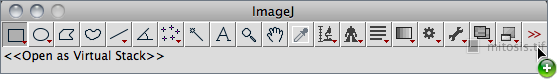
\includegraphics[scale=0.55]{images/DragAndDropVirtualTiff}
\end{infobox}



\subsection*{Hyperstacks\label{sub:Hyperstacks-Intro}}

\index{Stacks!Hyperstacks}Hyperstacks are multidimensional images,
extending image stacks to four (4D) or five (5D) dimensions: $x$
(width), $y$ (height), $z$ (slices), $c$ (channels or wavelengths)
and $t$ (time frames). Hyperstacks are displayed in a window with
three labelled scrollbars (\emph{see} \nameref{fig:Stacks-and-Hyperstacks}).
Similarly to the scrollbar in \nameref{sub:Stacks-Intro}, the frame
slider (\emph{t}) has a play/pause icon. 


\calso{\userinterface{\textsf{Image}\lyxarrow{}\nameref{sub:Hyperstacks}}
submenu}


\section[Color Images]{Color Images%
\footnote{This section is partially extracted from the MBF\,ImageJ online manual
at \protect\url{http://www.macbiophotonics.ca/imagej/colour_image_processi.htm}.%
}\label{sec:Color-Images}}

\index{MBF ImageJ}ImageJ deals with color mainly in three ways: pseudocolor
images, RGB images, RGB/ HS{\small B\nomenclature{HSB}{Hue Saturation Brightness}}
stacks, and composite images.\index{Image types}


\subsection*{Pseudocolor Images\label{sub:Pseudocolor-Images}}

A pseudocolor (or indexed color) image is a single channel gray image
(8, 16 or 32--bit) that has color assigned to it via a lookup table
or LUT\nomenclature{LUT}{Lookup table}\index{LUT}. A LUT is literally
a predefined table of gray values with matching red, green and blue
values so that shadows of gray are displayed as colorized pixels.
Thus, differences in color in the pseudo-colored image reflect differences
in intensity of the object rather than differences in color of the
specimen that has been imaged.

8-bit indexed color images (such as GIFs) are a special case of pseudocolor
images as their lookup table is stored in the file with the image.
These images are limited to 256 colors (24--bit RGB images allow 16.7
million of colors, \emph{see} \nameref{sec:Image-Types}) and concomitantly
smaller file sizes. Reduction of true color values to a 256 \index{Color palette@Color palette \see{LUT,}}color
palette is performed by color quantization algorithms. ImageJ uses
the \index{Color!Quantization}\index{Heckbert quantization}\index{Algorithm!Heckbert quantization}Heckbert's
median-cut color quantization algorithm (\emph{see} \userinterface{Image\lyxarrow{}\nameref{sub:Type}}
menu), which, in most cases, allows indexed color images to look nearly
identical to their 24-bit originals.


\calso{\userinterface{\textsf{Image}\lyxarrow{}\nameref{sub:Lookup-Tables}}
and \nameref{sub:LUTMenu}}


\subsection*{True Color Images\label{sub:True-color-images}}

As described in \nameref{sec:Image-Types}, true color images such
as RGB images reflect genuine colors, i.e., the green in an RGB image
reflects green color in the specimen. Color images are typically produced
by color CCD\nomenclature{CCD}{Charge-Coupled Device} cameras, in
which \index{Color filter array}color filter arrays (\href{http://en.wikipedia.org/wiki/Bayer_filter}{Bayer masks})
are placed over the image sensor.\index{CCD}


\subsubsection*{Color Spaces and Color Separation\label{sub:Color-Spaces-and}}

\href{http://en.wikipedia.org/wiki/Color_space}{Color spaces} \index{Color!Models}describe
the gamut of colors that image-handling devices deal with. Because
human vision is trichromatic, most color models represent colors by
three values. Mathematically, these values (color components) form
a three-dimensional space such as the RGB\index{RGB}, \index{HSB}HSB,
\index{CIE Lab}CIE\,Lab or \index{YUV}YUV color space. 
\begin{figure}[h]
\noindent 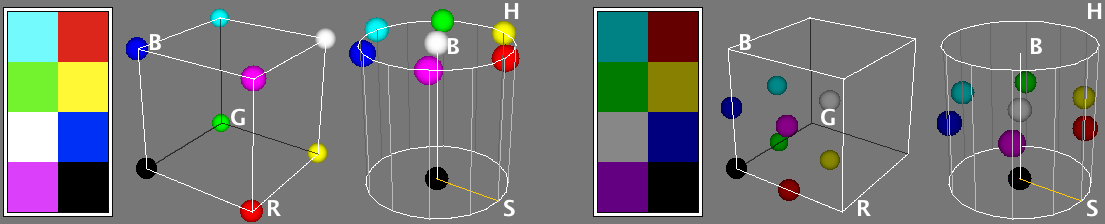
\includegraphics[width=1\columnwidth]{images/RGB-HSBcolorModels}\caption[RGB and HSB color models]{\textbf{\label{fig:ColorModels}Representation of an eight pixel
color image in the RGB and HSB color spaces.} The RGB color space
maps the RGB color model to a cube with \emph{Red} (R) values increasing
along the x-axis, \emph{Green} (G) along the y-axis and \emph{Blue}
(B) along the z-axis. In the HSB cylindrical coordinate system, the
angle around the central vertical axis corresponds to \emph{Hue} (H),
the distance from the axis corresponds to \emph{Saturation} (S), and
the distance along the axis corresponds to \emph{Brightness} (B).
In both cases the origin holds the black color. The right panel shows
the same image after brightness reduction, easily noted by the vertical
displacement along the HSB cylinder. Images produced using Kai Uwe
Barthel's \protect\href{http://www.f4.fhtw-berlin.de/~barthel/ImageJ/ColorInspector//help.htm}{3D Color Inspector}
plugin.}
\end{figure}


RGB (\uline{R}ed, \uline{G}reen, \uline{B}lue) is the most
commonly-used color space. However, other alternatives such as HSB
(\uline{H}ue, \uline{S}aturation, \uline{B}rightness) provide
significant advantages when processing color information. In the HSB
color space, \emph{Hue} describes the attribute of pure color, and
therefore distinguishes between colors. \emph{Saturation} (sometimes
called ``purity'' or ``vibrancy'') characterizes the shade of
color, i.e., how much white is added to the pure color.\emph{ Brightness}
(also know as \emph{Value} -- HSV system) describes the overall brightness
of the color (\emph{see} e.g., the color palette of \nameref{fig:CPtool}).
In terms of digital imaging processing, using the HSB system over
the traditional RGB is often advantageous: e.g., since the Brightness
component of an HSB image corresponds to the grayscale version of
that image, processing only the brightness channel in routines that
require grayscale images is a significant computational gain%
\footnote{\emph{See} Wootton R, Springall DR, Polak JM. Image Analysis in Histology:
Conventional and Confocal Microscopy. \emph{Cambridge University Press},
1995\emph{,} ISBN 0521434823%
}. You can read more about the HSB color model \href{http://en.wikipedia.org/wiki/HSB_color_space}{here}.

In ImageJ, conversions between image types are performed using the
\userinterface{\textsf{\small Image}\lyxarrow{}\nameref{sub:Type}}
submenu. Segmentation on the HSB, RGB, CIE\,Lab and YUV color spaces
can be performed by the \userinterface{\textsf{\small Image}\lyxarrow{}Adjust\lyxarrow{}\nameref{sub:Color-Threshold...}}
command \cite{C-ColorThres}. Segregation of color components (specially
useful for quantification of \index{Color!Deconvolution}\index{Color!Separation@Separation \see{Color!Deconvolution,}}\index{Immunohistochemistry@Immunohistochemistry \see{Histochemical staining,}}histochemical
staining) is also possible using Gabriel Landini's \href{http://www.dentistry.bham.ac.uk/landinig/software/cdeconv/cdeconv.html}{Colour Deconvolution}
plugin. In addition, several other plugins related to color processing
can be obtained from the \href{http://imagej.nih.gov/ij/plugins/index.html\#color}{ImageJ website}.


\subsubsection*{Conveying Color Information\textmd{}%
\footnote{This section is partially extracted from Masataka Okabe and Kei Ito,
\emph{Color Universal Design (CUD) --- How to make figures and presentations
that are friendly to Colorblind people}, \protect\url{http://jfly.iam.u-tokyo.ac.jp/color/},
accessed 2009.01.15%
}\label{sub:Conveying-Color-Information}}

People see color with significant variations. Indeed, the popular
phrase ``One picture is worth ten thousand words'' may not apply
to certain color images, specially those that do not follow the basic
principles of \href{http://jfly.iam.u-tokyo.ac.jp/color/}{Color Universal Design}.
Citing Masataka Okabe and Kei Ito:
\begin{quotation}
\index{Color!Blindness}Colorblind people can recognize a wide ranges
of colors. But certain ranges of colors are hard to distinguish. The
frequency of colorblindness is fairly high. One in 12 Caucasian (8\%),
one in 20 Asian (5\%), and one in 25 African (4\%) males are so-called
`red--green' colorblind.

There are always colorblind people among the audience and readers.
There should be more than \textsc{ten} colorblind in a room with 250\,people
(assuming 50\% male and 50\% {\small female}).

{[}\,\ldots{}{]} There is a good chance that the paper you submit
may go to colorblind reviewers. Supposing that your paper will be
reviewed by three white males (which is not unlikely considering the
current population in science), the probability that at least one
of them is colorblind is whopping 22\%! 
\end{quotation}
\begin{figure}
\noindent 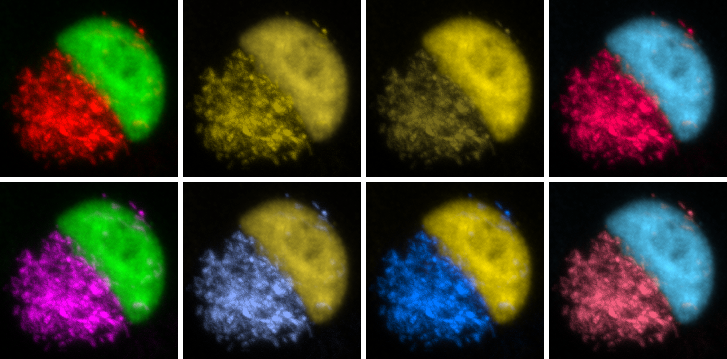
\includegraphics[width=1\columnwidth]{images/Dichromacy}\caption[Red--green images and partial color blindness]{\textbf{\label{fig:ColorBlindness}Red--green images and partial
color blindness.} Deuteranopia (second panel), protanopia (third panel)
are the most common types of partial color blindness (red\,/\,green
confusion). Tritanopia (blue\,/\,orange confusion, fourth panel)
is quite rare. \nameref{infobox:Replacing-Red-w-Magenta} (bottom
row) is a simple way to compensate for color vision deficiencies.}
\end{figure}
One practical point defined by the \href{http://jfly.iam.u-tokyo.ac.jp/color/}{Color Universal Design}
is the use of magenta in red--green overlays (\emph{see also} \cite{Landini:2009p19625}).
Magenta is the equal mixture of red and blue. Colorblind people that
have difficulties recognizing the red component can easily recognize
the blue hue. The region of double positive becomes white, which is
easily distinguishable for colorblind. In ImageJ this is easily accomplished
using the \userinterface{Image\lyxarrow{}Color\lyxarrow{}\nameref{sub:Merge-Channels...}},
or using the ImageJ macro language (\emph{see} \ref{infobox:Replacing-Red-w-Magenta}
\nameref{infobox:Replacing-Red-w-Magenta}). 
\begin{infobox}
\caption{\label{infobox:Replacing-Red-w-Magenta}Replacing Red with Magenta
in RGB Images}


When building RGB images, magenta can be obtained using the \userinterface{Image\lyxarrow{}Color\lyxarrow{}\nameref{sub:Merge-Channels...}}
Previously created RGB images can be converted to \index{Magenta Green Blue (MGB)}`MGB'
using \userinterface{Image\lyxarrow{}Color\lyxarrow{}\nameref{sub:Channels...[Z]}}.
Alternatively, the \textsf{\userinterface{\textsf{Process\lyxarrow{}\nameref{sub:Image-Calculator...}}}}
command can be used to add the red channel to the blue channel. Both
these approaches can be automated using the ImageJ macro language
as exemplified by Macros \eqref{lis:RGBtoMGB1} and \eqref{lis:RGBtoMGB2}.
Once saved in the \dirnameref{ImageJ/plugins/} folder these \nameref{sub:Macros-ExtendingIJ}
are treated as regular ImageJ commands.\medskip{}


In \nameref{sub:Fiji-intro}, as expected, the procedure of modifying
RGB images is simpler: one just needs to run \textsf{\userinterface{\textsf{Image\lyxarrow{}Color\lyxarrow{}Replace Red with Magenta}}}.
For even more convenience, Fiji provides an analogous command that
replaces the system clipboard's image with a magenta-green one.
\end{infobox}


It is also possible to simulate color blindness using the \href{http://www.vischeck.com/downloads/}{Vischeck}
or \href{http://www.dentistry.bham.ac.uk/landinig/software/dichromacy/dichromacy.html}{Dichromacy}
plugins%
\footnote{One advantage of Dichromacy over the Vischeck plugin is that it can
be recorded and called from scripts and macros, without user interaction.%
}, or in \index{Fiji}\nameref{sub:Fiji-intro}, using the \userinterface{Image\lyxarrow{}Color\lyxarrow{}Simulate Color Blindness}
command.
\begin{lstlisting}[caption={Replace\,Red\,with\,Magenta.ijm (Using \protect\userinterface{Process\lyxarrow{}Image Calculator\ldots{}})},label={lis:RGBtoMGB2},float=h,showstringspaces=false,tabsize=4]
 /* This macro replaces Red with Magenta in RGB images using Process>Image Calculator...  command. */
   if (bitDepth!=24)
       exit("This macro requires an RGB image");
 setBatchMode(true);
   title= getTitle();
   r= title+" (red)"; g= title+" (green)"; b= title+" (blue)";
   run("Split Channels");
   imageCalculator("Add", b, r);
   run("Merge Channels...", "red=&r green=&g blue=&b");
   rename(title + " (MGB)");
 setBatchMode(false);
\end{lstlisting}



\subsection*{Color Composite Images\label{sub:Color-Composites}}

In a \index{Color!Composites}composite image colors are handled through
channels. The advantages with this type of image over plain RGB images
are: 
\begin{enumerate}
\item Each channel is kept separate from the others and can be turned on
and off using the `Channels' tool (\textsf{\userinterface{\textsf{Image\lyxarrow{}Color\lyxarrow{}\nameref{sub:Channels...[Z]}}}}).
This feature allows, e.g., to perform measurements on a specific channel
while visualizing multiple. 
\item Channels can be 8, 16 or 32--bit and can be displayed with any lookup
table
\item More than 3\,channels can be merged or kept separate
\end{enumerate}
\begin{lstlisting}[caption={Replace\,Red\,with\,Magenta.ijm (Using \protect\userinterface{Image\lyxarrow{}Color\lyxarrow{}Channels\ldots{}})},label={lis:RGBtoMGB1},float=h,showstringspaces=false,tabsize=4]
 /* This macro replaces Red with Magenta in RGB images using the Image>Color>Channels... tool. */
   if (bitDepth!=24)         // Ignore non-RGB images
       exit("This macro requires an RGB image");
 setBatchMode(true);         // Enter `Batch' mode
   title = getTitle();       // Retrieve the image title
   run("Make Composite");    // Run Image>Color>Make Composite
   run("Magenta");           // Run Image>Lookup Tables>Magenta on channel 1
   run("RGB Color");         // Run Image>Type>RGB Color
   rename(title + " (MGB)"); // Rename the image
 setBatchMode(false);        // Restore `GUI' mode
\end{lstlisting}



\section{Selections\label{sec:Selections-Intro}}

Selections (regions of interest, ROIs\nomenclature{ROI}{Region Of Interest}),
are typically created using the \nameref{sub:Toolbar} \nameref{sec:IJ-Tools}.
Although ImageJ can display simultaneously several \index{Selection}\index{ROI@ROI \see{Selection,}}ROIs
(see \nameref{sub:Overlay-Intro} and \nameref{fig:The-ROI-Manager})
only one selection can be active at a time. Selections can be measured
(\textsf{\userinterface{\textsf{Analyze\lyxarrow{}}\nameref{sub:Measure...[m]}}}),
drawn (\userinterface{\textsf{Edit\lyxarrow{}}\nameref{sub:Draw-[d]}}),
filled (\textsf{\userinterface{\textsf{Edit\lyxarrow{}}\nameref{sub:Fill-[f]}}})
or filtered (\userinterface{\textsf{Process\lyxarrow{}}\nameref{sub:Filters}}
submenu), in the case of area selections. In addition it is also possible
to hold multiple ROIs as non-destructive \nameref{sub:Overlay-Intro}.

Selections can be initially outlined in one of the nine ImageJ default
colors (\emph{Red}, \emph{Green}, \emph{Blue}, \emph{Magenta}, \emph{Cyan},
\emph{Yellow}, \emph{Orange}, \emph{Black} and White). Once created,
selections can be contoured or painted with any other color using\textsf{
\userinterface{\textsf{Edit\lyxarrow{}Selection\lyxarrow{}}\nameref{sub:Properties...}}}.
Selection Color can be changed in \userinterface{\textsf{Edit\lyxarrow{}Options\lyxarrow{}}\nameref{sub:Colors...}},
by double clicking on the \nameref{sec:Point-Tool}, or using hot
keys (\emph{see} \eqref{lis:ChangeSelectionColor} \nameref{lis:ChangeSelectionColor}).
It is highlighted in the center of the \nameref{sec:Point-Tool} and
\nameref{sec:Multi-point-Tool}.
\begin{figure}[h]
\noindent 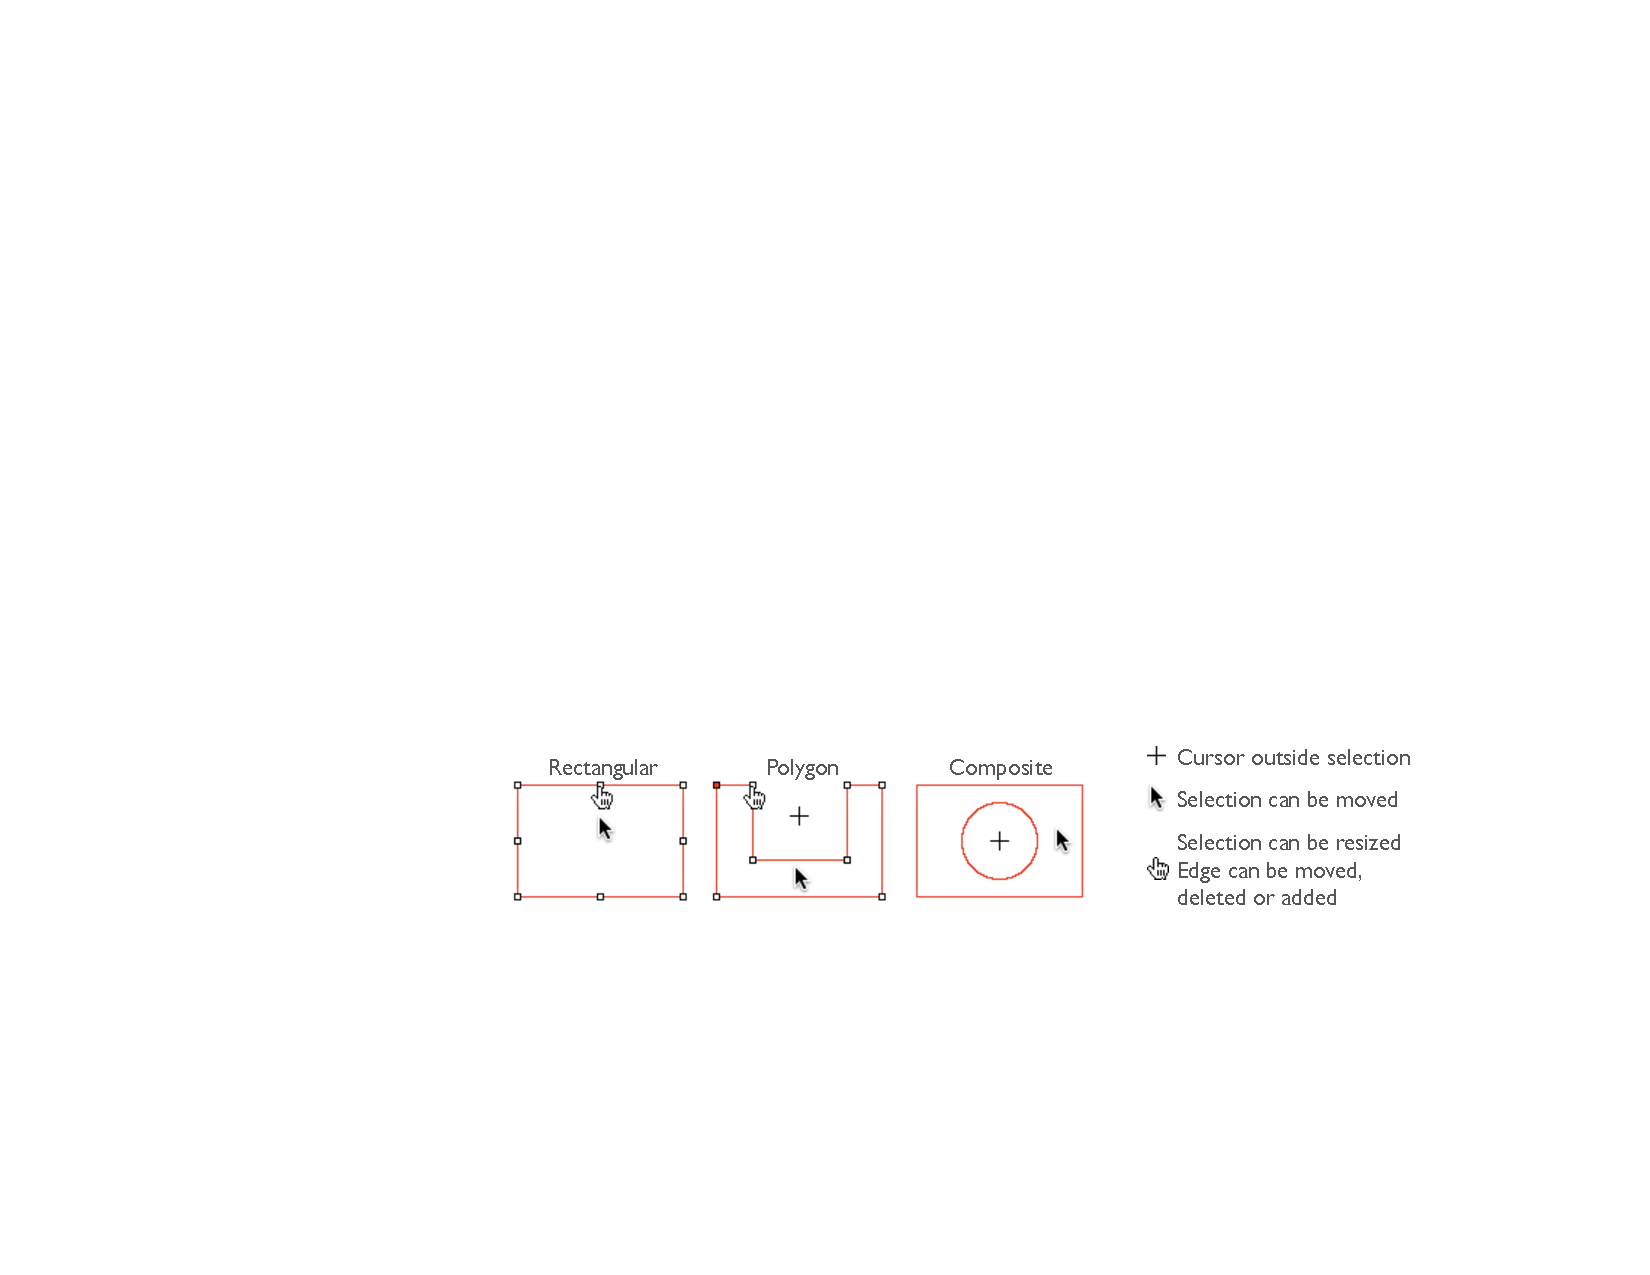
\includegraphics[width=0.88\columnwidth]{images/Selections}\caption{\textbf{\label{fig:exampleAreaROIs}Three types of area selections
In ImageJ.} Notice the cursor changes: to an \emph{arrow} when it
is within the selection, to a \emph{cross-hair} when outside the selection,
to a \emph{hand} when over a selection vertex or `handler'. Notice
also the filled handler in the polygon selection and the absence of
point handlers in \nameref{sub:Composite-selections}. \nameref{sub:Overlay-Intro},
i.e., non-active selections displayed in the non-destructive image
overlay, are also displayed without handlers.}
\end{figure}



\subsection{Manipulating ROIs\label{sub:Manipulating-ROIs}}

Most of commands that can be useful in defining or drawing selections
are available in the \textsf{\userinterface{\textsf{Edit\lyxarrow{}}\nameref{sub:SelectionSubMenu}}}
submenu and summarized in \nameref{fig:ROI-manipulations}. Listed
below are the most frequent manipulations involving \index{ROI@ROI \seealso{Selection,}}selections:
\begin{lyxlist}{00000000000}
\item [{\textbf{Adjusting}}] \noindent Area selections can be adjusted
with the \nameref{sub:Brush-Selection-Tool}. In addition, vertexes
of selections created with the \nameref{sub:Polygon-Selection-Tool}
and \nameref{sub:Segmented-Line-Selection} can be adjusted by Alt/Shift-clicking.
\item [{\textbf{Deleting}}] \noindent Choose any of the selection tools
and click outside the selection, or use \textsf{\userinterface{\noindent \textsf{Edit\lyxarrow{}Selection\lyxarrow{}}\nameref{sub:Select-None-[A]}}}.
Use\textsf{ \userinterface{\noindent \textsf{Edit\lyxarrow{}Selection\lyxarrow{}}\nameref{sub:Restore-Selection-[E]}}}
to restore a selection back after having deleted it. With \nameref{sub:Overlay-Intro},
an activated ROI can be deleted by pressing the \mykeystroke{\noindent Backspace}
(\mykeystroke{\noindent Delete} on Mac) key.
\item [{\textbf{Managing}}] \noindent A selection can be transferred from
one image window to another by activating the destination window and
runnig \textsf{\userinterface{\noindent \textsf{Edit\lyxarrow{}Selection\lyxarrow{}}\nameref{sub:Restore-Selection-[E]}}}.
Alternatively, \textsf{\userinterface{\noindent \textsf{Analyze\lyxarrow{}Tools\lyxarrow{}}\nameref{sub:SynchronizeWindows}}}
to create ROIs across multiple images. Multiple selections can be
stored as \nameref{sub:Overlay-Intro} or in the \nameref{fig:The-ROI-Manager}
list (\textsf{\userinterface{\noindent \textsf{Analyze\lyxarrow{}Tools\lyxarrow{}}\nameref{sub:ROI-Manager...}}}).
\item [{\textbf{Moving}}] \noindent Selections can be moved by clicking
and dragging as long as the cursor is within the selection and has
changed to an\ 
\includegraphics[scale=0.5]{images/pointers/Pointer-Arrow}.
The status bar displays the coordinates of the upper left corner of
the selection (or the bounding rectangle for non-rectangular selections)
as it is being moved. To move the contents of a selection, rather
than the selection itself, \textsf{\userinterface{\noindent \textsf{Edit\lyxarrow{}\nameref{sub:Copy[c]}}}},
\textsf{\userinterface{\noindent \textsf{Edit\lyxarrow{}\nameref{sub:Paste[v]}}}},
and then click within the selection and drag.
\item [{\textbf{Nudging}}] \noindent Selections can be `nudged' one pixel
at a time in any direction using the arrow keys. Note that the up
and down keys zoom the image in and out in the absence of selections
(\emph{see} \nameref{Arrow-Keys} shortcuts).
\item [{\textbf{Resizing}}] The \nameref{sub:Brush-Selection-Tool} can
be used to perform fine adjustments of ROI contours. Most ROIs can
be resized one pixel at a time by holding \mykeystroke{Alt} while
using the arrow keys. In general (\emph{see} \nameref{sec:Area-selection-tools}
and \nameref{sec:Line-Selection-Tools} for details), selections are
resized by dragging one of the selection handlers. While dragging,
holding \mykeystroke{Ctrl} resizes the selection around its center,
holding \mykeystroke{Alt} imposes a fixed aspect ratio and holding
\mykeystroke{Shift} forces a 1:1 aspect ratio.
\end{lyxlist}

\calso{\nameref{sec:Key-Modifiers}}


\subsection{Composite Selections\label{sub:Composite-selections}}

\begin{wrapfigure}[5]{l}{0.245\columnwidth}%

\includegraphics[scale=0.6]{images/compositeROI}\end{wrapfigure}%
Composite selections are non-contiguous ROIs containing more than
one cluster of pixels and/or ROIs containing internal holes. Composite
ROIs are typically originated with the \nameref{sub:Brush-Selection-Tool}
but they can be defined with any other selection tool using key modifiers. 

The following modifier keys can be use to create composite selections:\index{Selection!Composite}
\begin{lyxlist}{shifttt}
\item [{\mykeystroke{Shift}}] \noindent Drawing outside current selection
while pressing Shift creates new content. To add a non-square rectangle
or ellipse, the Shift key must be released after adding the selection
\item [{\mykeystroke{Alt}}] Drawing inside current selection while pressing
Alt creates a hole removing content from the ROI
\end{lyxlist}
Note that some operations may not be performed properly on complex
ROIs. In these cases, it may be useful to convert a composite ROI
into a polygon using the \userinterface{Edit\lyxarrow{}Selection\lyxarrow{}\nameref{sub:Enlarge...}}
command as explained in \ref{infobox:Composites} \nameref{infobox:Composites}.


\calso{\nameref{sub:Wand-Tool}, \href{http://imagejdocu.tudor.lu/doku.php?id=wishlist:completed:freehand_and_selection_brush_roi_conversion}{ROI2PolylineROI}
macro}


\subsection[Selections With Sub-pixel Coordinates]{Selections With Sub-pixel Coordinates\label{sub:Sub-pixel-Selections}\index{Sub-pixel selections}\feature{Selections with sub-pixel resolution}}

Since ImageJ 1.46, selections can be defined with \href{http://en.wikipedia.org/wiki/Sub-pixel_resolution}{subpixel accuracy},
beyond the nominal pixel resolution of the image: \nameref{fig:Subpixel-selections}.
Line Selections (\emph{see} \nameref{sec:Line-Selection-Tools}) are
created with floating-point coordinates if the \emph{Sub-pixel resolution}
checkbox is active in \userinterface{Edit\lyxarrow{}Options\lyxarrow{}\nameref{sub:Profile-Plot-Options...}}
Sub-pixel coordinates of pre-existing selections can be interpolated
using the \userinterface{Edit\lyxarrow{}Selection\lyxarrow{}\nameref{sub:Interpolate}}
command. Interpolated points are easily noticeable on small selections
created on images zoomed 1200\% or greater.
\begin{figure}[h]
\noindent 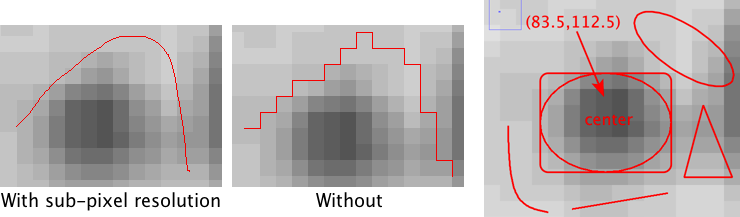
\includegraphics[scale=0.45]{images/SubPixel}\caption[Floating point selections]{\label{fig:Subpixel-selections}\textbf{Interpolated selections.}
ROIs drawn with (left) or without (middle) sub-pixel accuracy. For
line selections (\emph{see} \nameref{sec:Line-Selection-Tools}),
this option can be enabled in\textbf{ }\protect\userinterface{Edit\lyxarrow{}Options\lyxarrow{}\nameref{sub:Profile-Plot-Options...}}
by activating the \emph{Sub-pixel resolution} checkbox. Pixel coordinates
of area selections (\emph{see} \nameref{sec:Area-selection-tools}),
can be interpolated using \protect\userinterface{Edit\lyxarrow{}Selection\lyxarrow{}\nameref{sub:Interpolate}}.
The image on the right is the output of \protect\filenameref{\protect\href{http://imagej.nih.gov/ij/macros/js/SubPixelSelections.js}{SubPixelSelections.js}},
a script that demonstrates how to create selections at sub-pixel resolution
without the need of setting any option in ImageJ.}
\end{figure}



\calso{\nameref{sub:Zoom}, \nameref{sec:Magnifying-Glass}}


\section[Overlays]{Overlays\label{sub:Overlay-Intro}\improvement{Improved handling of Overlays}}

\index{Overlay}\index{Non-destructive annotations@Non-destructive annotations \see{Overlay,}}\index{Annotations!Non-destructive image overlay}Overlays
are non-active selections displayed `over' the pixel data, on the
image overlay, and are the core of non-destructive image processing
in ImageJ. In a way you can think of the image overlay as an invisible
\nameref{fig:The-ROI-Manager} in which selections are being added,
allowing ROIs to be on `hold'. This concept of multiple distinct
selections has been dramatically improved in \nameref{sub:ImageJ2intro}
so we urge you to download IJ2 if multiple ROIs are important in your
workflows.
\begin{figure}
\noindent 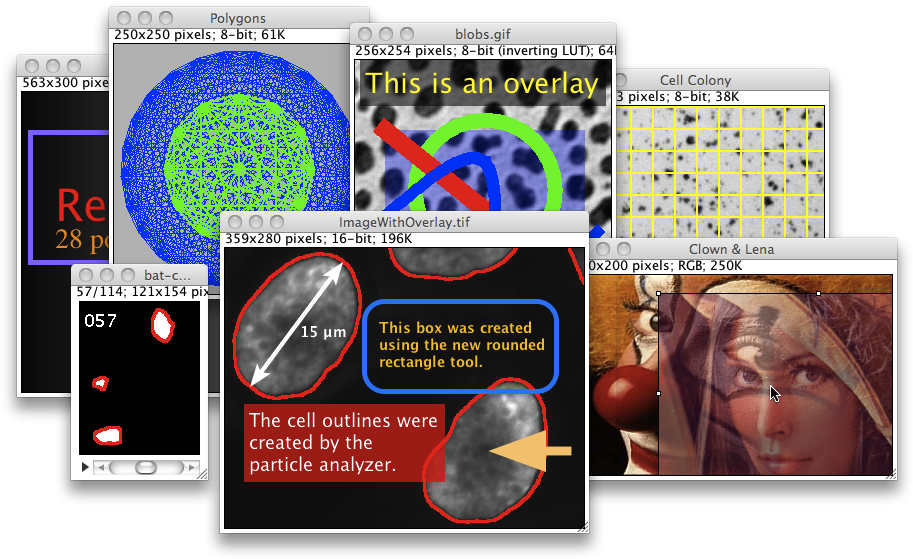
\includegraphics[width=0.75\columnwidth]{images/OverlayShowcase}\caption{\textbf{Non-destructive operations using the image overlay.} Overlays
can be used to annotate images, store ROIs and blend images (ImageROIs)
at multiple opacity levels. Refer to the \protect\userinterface{Image\lyxarrow{}\nameref{sub:Overlay}}documentation
for further \nameref{fig:image-overlays}. You can \protect\href{http://imagej.nih.gov/ij/docs/guide/images/ImageWithOverlay.tif}{download the frontmost}
image to practice overlay editing. }
\end{figure}


Importantly, overlay selections are \href{http://en.wikipedia.org/wiki/Vector_graphics}{vector graphics}
composed of mathematically-defined paths (as opposed to \href{http://en.wikipedia.org/wiki/Raster_graphics}{raster graphics}
in which objects are defined by pixels) and are not affected by scaling,
i.e., do not become pixelated. Most of overlay-related commands are
listed in the \userinterface{Image\lyxarrow{}\nameref{sub:Overlay}},
and in the ROI Manager window (\userinterface{Analyze\lyxarrow{}Tools\lyxarrow{}\nameref{sub:ROI-Manager...}}).
Appearance of overlay selections can be adjusted using \userinterface{Image\lyxarrow{}Overlay\lyxarrow{}\nameref{sub:Overlay-Options...}}/\userinterface{\nameref{sub:Labels...}}

As mentioned in \ref{infobox:Formats} \nameref{infobox:Formats},
overlays are saved in the header of tif images, and do not need to
be saved externally when using TIFF, the default file format of ImageJ.
The major advantages of overlays are summarized below:
\begin{description}
\item [{Storage\ of\ ROIs}] In ImageJ it is only possible to have a single
ROI at a time. However, it is possible to add selections to the image
overlay using \mykeystroke{B} (\userinterface{Image\lyxarrow{}Overlay\lyxarrow{}\nameref{sub:Add-Selection...[b]}}).\feature{}
Once added to the image overlay, ROIs can be re-activated by Alt-clicking,
Control-clicking or long-pressing ($\nicefrac{1}{4}$ second or longer).
Activated ROIs can be deleted by pressing the \mykeystroke{\noindent Backspace}
key. Selections can also be added and recovered in bulk, using the
\userinterface{Image\lyxarrow{}Overlay\lyxarrow{}\nameref{sub:From-ROI-Manager}}/\userinterface{\nameref{sub:To-ROI-Manager}}
commands.
\item [{Non-destructive\ annotations}] Overlays are the best way of annotating
images in ImageJ (\nameref{fig:image-overlays}). As vector graphics,
overlays do not change pixel values, can be scaled without loss of
quality even at high zoom levels (\emph{see} \ref{infobox:ZoomedCanvas}
\nameref{infobox:ZoomedCanvas}) and can be displayed at different
opacity values (\emph{see} \ref{infobox:HEX} \nameref{infobox:HEX}).
RGB snapshots of the image with embedded overlays can be created by
holding \mykeystroke{Shif} \mykeystroke{F}, the shortcut for \userinterface{Image\lyxarrow{}Overlay\lyxarrow{}\nameref{sub:Flatten-[F]}}.
`Flattened' images with the overlay rendered as pixel data are also
created when saving the image as PNG or JPEG (\userinterface{File\lyxarrow{}\nameref{sub:SaveAs}}),
or when printing the image canvas (\userinterface{File\lyxarrow{}\nameref{sub:Print...[p]}}).
The \userinterface{Flatten} command is also listed in the \nameref{fig:The-ROI-Manager}.
\item [{Image\ ROIs}] An \index{Image selection@Image selection \see{ImageROI}}\index{ImageROI}imageROI
(image selection) is a ROI that displays an image as an overlay. As
described in \userinterface{Edit\lyxarrow{}Selection\lyxarrow{}\nameref{sub:Image-to-Selection...}}
and \userinterface{Image\lyxarrow{}Overlay\lyxarrow{}\nameref{sub:Add-Image...}},
this allows multiple images to be \index{Blend}blended on a single
image canvas.
\end{description}

\section{3D Volumes\label{sub:3D-Intro}}

Currently, the support for \index{ThreeD ROIs@3D ROIs}\index{3D ROIs}3D
ROIs (selections containing contiguous cluster of voxels) is somewhat
limited in ImageJ. This limitation has been addressed by \nameref{sub:ImageJ2intro}
and several IJ1 plugins. The list below summarizes some of the ImageJ
plugins that deal effectively with multi-dimensional objects. Note
that a manual installation of these tools as standalone ImageJ plugins
is a challenging task given their special dependencies, reason why
they are all bundled as part of \index{Fiji}\nameref{sub:Fiji-intro}.
\begin{figure}
\noindent 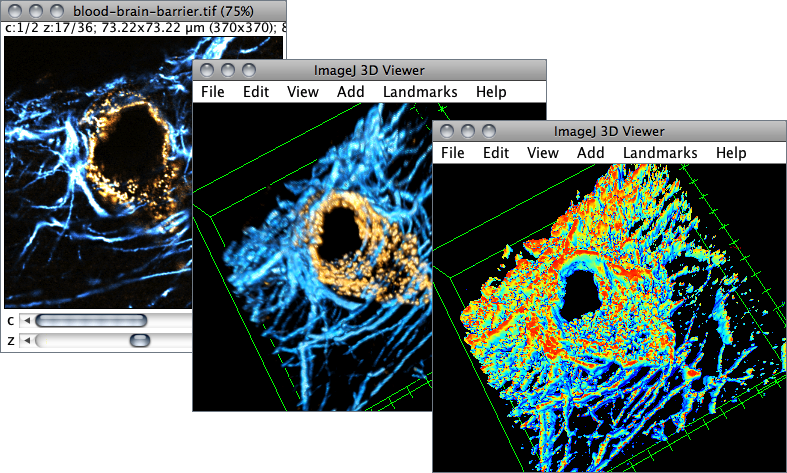
\includegraphics[width=0.7\columnwidth]{images/3Dviewer}\caption[3D Viewer]{\label{fig:-3D-Viewer}\textbf{3D Viewer (Fiji\,1.46o), bringing
hardware-accelerated 3D visualization to ImageJ.} As explained in
\nameref{sub:3D-Intro}, most of plugins that truly extend ImageJ
functionally to multi-dimentional data are bundled as part of Fiji.}
\end{figure}

\begin{description}
\item [{3D\ Filters}] Specialized \index{ThreeD Filters@3D Filters}\index{3D Filters}3D
filters such as \userinterface{Process\lyxarrow{}Filters\lyxarrow{}\nameref{sub:Gaussian-Blur-3D...}}
can be installed to perform 3D operations. Examples are the \href{http://imagejdocu.tudor.lu/doku.php?id=plugin:morphology:3d_binary_morphological_filters:start}{3D processing package}
by Thomas Boudier \cite{Iannuccelli:2010p13791} and the \href{http://fiji.sc/wiki/index.php/3D_Binary_Filters}{3D binary filters}
by Benjamin Schmid.
\item [{3D\ Object\ Counter}] \href{http://imagejdocu.tudor.lu/doku.php?id=plugin:analysis:3d_object_counter:start}{3D Object Counter}
(3D-OC) \index{ThreeD Object Counter@3D Object Counter}\index{3D Object Counter}counts
and qualifies 3D objects in a stack \cite{Bolte:2006p2466}, similarly
to the 2D analysis performed by \userinterface{Analyze\lyxarrow{}\nameref{sub:Analyze-Particles...}}
It is complemented by \href{http://imagejdocu.tudor.lu/doku.php?id=plugin:stacks:3d_roi_manager:start}{3D Roi Manager}
\cite{Iannuccelli:2010p13791}, a companion plugin that adds a 3D
\nameref{fig:The-ROI-Manager} to ImageJ
\item [{3D\ Viewer}] \href{http://3dviewer.neurofly.de/}{3D Viewer} \index{ThreeD Viewer@3D Viewer}\index{3D Viewer}brings
powerful hardware-accelerated 3D visualization to ImageJ \cite{Schmid:2010p18702},
extending the limited functionality of \userinterface{Image\lyxarrow{}Stacks\lyxarrow{}\nameref{sub:3D-Project...}}
In the ImageJ \nameref{fig:-3D-Viewer} stacks can be displayed as
texture-based volume renderings, surfaces or orthoslices. It is macro-recordable
and can be used by other plugins as a high-level programming library
for 3D visualization
\item [{Simple\ Neurite\ Tracer}] \href{http://fiji.sc/wiki/index.php/Simple_Neurite_Tracer}{Simple Neurite Tracer}
\index{Simple Neurite Tracer}allows semi-automated segmentation of
tubular structures in 3D \cite{Longair:2011p20768}
\item [{TrakEM2}] As mentioned earlier, \nameref{misc:TrakEM2} features
powerful tools for multi-dimensional regions of interest \cite{Cardona:2010p18306}
\end{description}

\calso{\userinterface{Image\lyxarrow{}Stacks\lyxarrow{}\nameref{sub:3D-Project...}}/\userinterface{\nameref{sub:Orthogonal-Views}},
\userinterface{Analyze\lyxarrow{}\nameref{sub:Surface-Plot...}},
\ref{infobox:Skeletonize-vs-Skeletonize3D} \nameref{infobox:Skeletonize-vs-Skeletonize3D},
\href{http://fiji.sc/wiki/index.php/Special:Search?search=3d&fulltext=Search}{3D tools in Fiji},
\href{http://www.longair.net/edinburgh/imagej/three-pane-crop/}{Three Pane Crop},
\href{http://imagejdocu.tudor.lu/doku.php?id=tutorial:working:3d_image_processing_and_analysis_with_imagej}{3D image processing tutorials}
on the ImageJ wikipage}


\section[Settings and Preferences]{Settings and Preferences\label{sec:Settings-and-Preferences}\improvement{}}

\index{Settings}\index{Preferences@Preferences \see{Settings,}}\index{Options@Options \see{Settings,}}ImageJ
preferences are automatically saved in a preferences file, the\texttt{
}\filenameref{IJ\_prefs.txt} text file. This file is stored in \dirnameref{$\sim$/Library/Preferences/}
on Mac OS\,X, in \dirnameref{$\sim$/.imagej/} on Linux and Windows
(with $\sim$ referring to the user's home directory). Several macros
and plugins also write parameters to this file. If the \filenameref{IJ\_prefs.txt}
is erased using \userinterface{Edit\lyxarrow{}Options\lyxarrow{}\nameref{sub:ResetOptions}},
ImageJ will create a new one the next time it is opened resetting
all parameters to their default values. 

Sometimes, it may be useful to override (or restore) certain settings
that may have been changed during a working session. For example,
the \emph{Limit to threshold} option (\userinterface{\textsf{Analyze\lyxarrow{}}\nameref{sub:Set-Measurements...}})
will affect most measurements performed on thresholded images. Thus,
it may be wise to check the status of this parameter before each analysis,
specially when working on multiple computers.

\begin{lstlisting}[caption={Ensuring Specific Settings at Launch},label={lis:setOption},float=h,showstringspaces=false,tabsize=4]
 macro "AutoRun" {
   setOption("DebugMode", true);
   setOption("Bicubic", true);
   setOption("Display Label", true);
   setOption("Limit to Threshold", false);
   setOption("BlackBackground", true);
   run("Colors...", "foreground=white background=black"); //this line could be substituted by: setBackgroundColor(0,0,0); setForegroundColor(255,255,255);
   run("Profile Plot Options...", "width=350 height=200 draw");
   run("Brightness/Contrast...");
 }
\end{lstlisting}
The \texttt{\code{\texttt{setOption()}}} \href{http://imagej.nih.gov/ij/developer/macro/functions.html\#setOption}{macro function}
can be used to set this and several other ImageJ options. Calling
this function from the \index{StartupMacros}\index{AutoRun}``AutoRun''
macro in the \filenameref{StartupMacros.txt} file ensures preferences
are set each time ImageJ starts. The macro \eqref{lis:setOption}
\nameref{lis:setOption} exemplifies this approach ensuring that the
following settings are enforced at startup:
\begin{enumerate}
\item TIFF tag values are displayed by ImageJ (\emph{Debug Mode} in \textsf{\userinterface{\textsf{Edit\lyxarrow{}Options\lyxarrow{}}\nameref{sub:Misc...}}})
\item Bicubic interpolation is preferred over bilinear (e.g.,\textsf{ }\userinterface{\textsf{Edit\lyxarrow{}Selection\lyxarrow{}}\nameref{sub:Straighten...}})
\item The name of the measured image name is recorded in the first column
of the \nameref{sec:Results-Table} (\emph{Display Label }in \userinterface{\textsf{Analyze\lyxarrow{}}\nameref{sub:Set-Measurements...}})
\item Measurements are not restricted to thresholded pixels (\emph{Limit
to Threshold} in \userinterface{\textsf{Analyze\lyxarrow{}}\nameref{sub:Set-Measurements...}})
\item Binary images are processed assuming white objects on a black background
(\emph{Black background} in \userinterface{\textsf{Process\lyxarrow{}Binary\lyxarrow{}}\nameref{sub:BinaryOptions...}},
\emph{see} \ref{infobox:blackBackground} \nameref{infobox:blackBackground})
\item \emph{Background color} is black and \emph{foreground color} is white
(\textsf{\userinterface{\textsf{Edit\lyxarrow{}Options\lyxarrow{}}\nameref{sub:Colors...}}})
\item ImageJ plots contain grid lines and are always $350\times200$\,pixels
in size (\textsf{\userinterface{\textsf{Edit\lyxarrow{}Options\lyxarrow{}}\nameref{sub:Profile-Plot-Options...}}})
\item Open the B\&C widget at its last saved screen position (\textsf{\userinterface{\textsf{Image\lyxarrow{}Adjust\lyxarrow{}}\nameref{sub:Brightness/Contrast...[C]}}})
\end{enumerate}

\calso{\nameref{sec:GUIcustomization}, FAQs\nomenclature{FAQ}{Frequently Asked Questions}
on \href{http://imagejdocu.tudor.lu/doku.php?id=faq:technical:how_do_i_set_up_imagej_to_deal_with_white_particles_on_a_black_background_by_default}{ImageJ wikipage},
\ref{infobox:Organizing-Commands} \nameref{infobox:Organizing-Commands} }


\clearpage{}

\thispagestyle{plain}


\part{Extending ImageJ\label{sec:Extending-ImageJ}}

ImageJ capabilities can be extended by loadable code modules in the
form of macros, scripts or plugins. 300$+$ macros, 500$+$ plugins
and 20$+$ scripts are available through the ImageJ web site. Below
is a short description of these three type of ImageJ add-ons:
\begin{lyxlist}{macrosss}
\item [{\nameref{sub:Macros-ExtendingIJ}}] \noindent The easiest way to
execute a series of ImageJ commands. The ImageJ \index{Macros}macro
language -- a \emph{Java-like} language -- contains a set of control
structures, operators and built-in functions and can be used to call
built-in commands and other macros. Macro code is stored in text files
(\filenameref{\noindent .txt} and \filenameref{\noindent .ijm} extensions).
\item [{\nameref{sub:Plugins}}] Much more powerful, flexible and faster
than macros (most of ImageJ's built-in menu commands are actually
\index{Plugins}plugins) but harder to write and debug. Plugins are
written in the \index{Java}Java programming language (\filenameref{.java}
source files) and compiled to \filenameref{.class} files.
\item [{\nameref{sub:Scripts}}] ImageJ uses the Mozilla Rhino interpreter
to run \index{JavaScript}JavaScripts. Similarly to plugins, scripts
have full access to all ImageJ and Java APIs but do not need to be
compiled (scripts and macros run interpretively). On the other hand,
scripts lack the simplicity of macro language and feel less integrated
in ImageJ.
\end{lyxlist}

\section{Macros\label{sub:Macros-ExtendingIJ}}

A \index{Macros}macro is a simple program that automates a series
of ImageJ commands. The easiest way to create a macro is to record
a sequence of commands using the command recorder (\textsf{\userinterface{\textsf{Plugins\lyxarrow{}Macros\lyxarrow{}}\nameref{sub:Record...}}}). 

A macro is saved as a text file (\filenameref{.txt }or \filenameref{.ijm}
extension) and once installed executed by selecting the macro name
in the \textsf{\userinterface{\textsf{Plugins\lyxarrow{}}\nameref{sub:Macros}}}
submenu, by \href{http://imagej.nih.gov/ij/developer/macro/macros.html\#shortcuts}{pressing a key}
or, in the case of \href{http://imagej.nih.gov/ij/developer/macro/macros.html\#tools}{Macro tools},
by clicking on an icon in the ImageJ toolbar. In addition, any macro
file placed in \dirnameref{ImageJ/plugins} with an \filenameref{.ijm}
extension will be installed in the \textsf{\userinterface{\textsf{Plugins\lyxarrow{}}}
}menu like any other plugin (before version\,1.41 only files with
an underscore in the name would be listed).

There are more than 300\,example macros, on the ImageJ Web site.
To try one, open it in a browser window and drag it directly to the
\nameref{fig:The-ImageJ-window} or, copy it to the clipboard (\mykeystroke{Ctrl}
\mykeystroke{A}, \mykeystroke{Ctrl} \mykeystroke{C}), switch to
IJ, and run \textsf{\userinterface{\textsf{File\lyxarrow{}New\lyxarrow{}}\nameref{sub:SystemClipboard[V]}}}
(\mykeystroke{Ctrl} \mykeystroke{Shift} \mykeystroke{V}), pasting
the macro into a new \nameref{sub:ImageJ-Macro-Editor} window. Run
it using the editor's \textsf{Macros\lyxarrow{}Run Macro} command
(\mykeystroke{Ctrl} \mykeystroke{R}). Most of the example macros
are also available in the macros folder, inside the ImageJ folder.


\subsection*{Macro Programming\label{sub:Macro-Programming}}

The ImageJ community has created excellent tutorials on macro programming.
These resources are indispensable guides to the ImageJ macro language: 
\begin{enumerate}
\item \emph{The ImageJ Macro Language --- Programmer's Reference Guide}
by J�r�me Mutterer and Wayne Rasband. This booklet compiles most of
the documentation dispersed throughout the web related to ImageJ's
macro programming. It provides an up to date printable manual for
the ImageJ macro language:\\
\url{http://imagej.nih.gov/ij/docs/macro_reference_guide.pdf}
\item \improvement{Fourtneen new macro functions}The Built-in Macro Functions
webpage (\textsf{\userinterface{\textsf{Help\lyxarrow{}}\nameref{sub:Macro-Functions...}}}
and \textsf{\userinterface{\textsf{Macros\lyxarrow{}}\nameref{FunctionFinder[F]}}}
in the \nameref{sub:ImageJ-Macro-Editor}) is the indispensable guide
to the built-in functions that can be called from the ImageJ macro
language. It is thoroughly documented and constantly updated:\\
\url{http://imagej.nih.gov/ij/developer/macro/functions.html}
\item Tutorials on the \index{Fiji}Fiji webpage: \\
\url{http://fiji.sc/wiki/index.php/Introduction_into_Macro_Programming}
\item How-tos and tutorials on the ImageJ Documentation Portal\\
\url{http://imagejdocu.tudor.lu/}
\end{enumerate}

\calso{\nameref{sub:Scripts}, \nameref{sub:Plugins}, \nameref{sub:ImageJ-Macro-Editor},
\nameref{sub:Fiji-Scrip-Editor}}


\section{Scripts\label{sub:Scripts}}

\index{JavaScript}JavaScript scripting was introduced in ImageJ\,1.41
in order to bring full access to ImageJ and Java APIs (\emph{see}
\nameref{tab:Advantages-JavaScript}). ImageJ uses the Mozilla Rhino
interpreter built into Java\,1.6 for Linux and Windows to run JavaScript.
Mac users, and users of earlier versions of Java, must download \filenameref{JavaScript.jar}
into the plugins folder. This JAR\nomenclature{JAR}{Java ARchive}
file is available on the \href{http://imagej.nih.gov/ij/download/tools/JavaScript.jar}{ImageJ website}
and is included with the Mac version of ImageJ in \dirnameref{ImageJ/plugins/jars}. 

Example JavaScript programs are available at \href{http://imagej.nih.gov/ij/macros/js/}{imagej.nih.gov/ij/macros/js/}.
Thread safe JavaScript code can be generated using the Recorder (\userinterface{Plugins\lyxarrow{}Macros\lyxarrow{}\nameref{sub:Record...}}).
Scripts can be opened in the editor as any other macro. Scripts with
the extension \filenameref{.js} can be run using \userinterface{Macros\lyxarrow{}Run Macro}
otherwise \userinterface{Macros\lyxarrow{}Evaluate JavaScript} (\mykeystroke{Ctrl}
\mykeystroke{J}) must be used.


\subsection*{JavaScript Programming}

Resources on ImageJ JavaScript scripting include:
\begin{enumerate}
\item The ImageJ web site, with growing documentation:\\
\url{http://imagej.nih.gov/ij/developer/javascript.html}
\item Tutorials on the \index{Fiji}Fiji webpage:\\
\url{http://fiji.sc/wiki/index.php/Javascript_Scripting}
\item Online scripts repository:\\
\url{http://imagej.nih.gov/ij/macros/js/}
\end{enumerate}
\selectlanguage{american}%
\begin{table}
\noindent \caption[\selectlanguage{english}%
Advantages and disadvantages of JavaScript\selectlanguage{english}%
]{\selectlanguage{english}%
\label{tab:Advantages-JavaScript}\textbf{Advantages and disadvantages
of JavaScript in ImageJ.} \index{ActionBar}\index{CodeBar} A thorough
comparison between different scripting languages is available on the
\protect\href{http://fiji.sc/wiki/index.php/Scripting_comparisons}{Fiji webpage}.\selectlanguage{english}%
}


\noindent {\scriptsize }%
\begin{minipage}[t]{1\columnwidth}%
\selectlanguage{english}%
\renewcommand{\arraystretch}{1.15}
\addtocounter{footnote}{1}
\begin{spacing}{0.9}

\noindent %
\begin{tabular}{>{\raggedright}p{0.476\columnwidth}>{\raggedright}p{0.476\columnwidth}}
\toprule 
\multicolumn{1}{>{\centering}m{0.476\columnwidth}}{{\small JavaScript Advantages}} & \multicolumn{1}{>{\centering}m{0.476\columnwidth}}{{\small JavaScript Disadvantages}}\tabularnewline
\midrule
{\small Full access to ImageJ and Java APIs} & {\small Slower, especially starting up}\tabularnewline
{\small \href{http://en.wikipedia.org/wiki/ECMAScript}{Standardized}} & {\small No equivalent of macro sets}\tabularnewline
{\small Richer language (objects, \code{{\small ?}} operator, \code{{\small break}},
\code{{\small continue}}, etc.)} & {\small Cannot use most of ImageJ's 360+ \href{http://imagej.nih.gov/ij/developer/macro/functions.html}{built in macro functions}}\tabularnewline
{\small \href{http://en.wikipedia.org/wiki/JavaScript}{Extensive documentation}} & {\small Requires knowledge of complex ImageJ and Java APIs}\tabularnewline
 & {\small No support for ``batch mode''}\tabularnewline
 & {\small Cannot create \nameref{sec:CustomToolsAndToolsets} and toolbar
menus}\tabularnewline
 & {\small Not compatible with \nameref{FunctionFinder[F]} and CodeBar}%
\footnote{{\small CodeBar is a convenient `ActionBar' that retrieves snippets
and common tasks frequently used in macro writing. `ActionBars'
provide one or many easy to use button bar(s) that extend ImageJ's
graphical user interface. You can read more about the ActionBar plugin
at the \href{http://imagejdocu.tudor.lu/doku.php?id=plugin:utilities:action_bar:start}{ImageJ Documentation Portal}.}%
}\tabularnewline
 & {\small No debugger}\tabularnewline
\end{tabular}

\end{spacing}\selectlanguage{english}%
%
\end{minipage}
\end{table}


\selectlanguage{english}%

\calso{\nameref{sub:Macros-ExtendingIJ}, \nameref{sub:Plugins}, \nameref{sub:ImageJ-Macro-Editor},
\nameref{sub:Fiji-Scrip-Editor}}


\section{Plugins\label{sub:Plugins}}

Plugins are a much more powerful concept than \nameref{sub:Macros-ExtendingIJ}
and \nameref{sub:Scripts} and most of ImageJ's built-in menu commands
are in fact implemented as \index{Plugins}plugins. Quoting Werner
Bailer \cite{Bailer:2006p14110}:
\begin{quotation}
Plugins are implemented as \index{Java}Java classes, which means
that you can use all features of the Java language, access the full
ImageJ API\nomenclature{API}{Application Programming Interface} and
use all standard and third-party Java APIs in a plugin. This opens
a wide range of possibilities of what can be done in a plugin. 

The most common uses of plugins are filters performing some analysis
or processing on an image or image stack and I/O plugins for reading/writing
not natively supported formats from/to file or other devices. But
as you can see when looking at the plugins listed on the ImageJ plugins
page, there are many other things you can do with plugins, such as
rendering graphics or creating extensions of the ImageJ graphical
user interface.
\end{quotation}
Plugins in the \dirnameref{ImageJ/plugins/} folder are listed at
the bottom of the \userinterface{\nameref{sec:Plugins}} menu (\emph{see}
\ref{infobox:Organizing-Commands} \nameref{infobox:Organizing-Commands}).
Only \filenameref{.class} and \filenameref{.jar} files in the plugins
folder with at least one underscore in their name will be installed.
Note that, with IJ\,1.44d an later, ImageJ no longer automatically
installs, at startup, plugins in JAR file directories that start with
a lower case letter. 


\subsection*{Developing ImageJ Plugins}

More information on how to develop ImageJ plugins can be obtained
on the following documents:
\begin{enumerate}
\item Developer Resources Page on the ImageJ website (\textsf{\userinterface{\textsf{Help\lyxarrow{}}\nameref{sub:Help-Dev.Resources...}}}):\\
\url{http://imagej.nih.gov/ij/developer/index.html}
\item Dedicated tutorials on \index{Fiji}Fiji's webpage:\\
\url{http://fiji.sc/wiki/index.php/Introduction_into_Developing_Plugins}
\item Dedicated tutorials on the ImageJ Documentation Portal:\\
\url{http://imagejdocu.tudor.lu/}
\item Dedicated tutorials on the ImageJDev webpage:\nomenclature{IDE}{Integrated Development Environment}\index{Eclipse}\index{NetBeans}\\
\url{http://developer.imagej.net/ides}
\end{enumerate}

\calso{\nameref{sub:Macros-ExtendingIJ}, \nameref{sub:Scripts}, \nameref{sub:ImageJ-Macro-Editor},
\nameref{sub:Fiji-Scrip-Editor}}


\section{Scripting in Other Languages\label{sec:ScriptingOtherLang}}

Support for other languages is possible in ImageJ using \nameref{sub:Fiji-intro}
and its powerful editor. Fiji adds extra support for \index{BeanShell}BeanShell,
\index{Clojure}Clojure, \index{Python}\index{Jython@Jython  \see{Python,}}Python
and \index{Ruby}Ruby. The following documents will introduce you
to the advanced scripting capabilities of Fiji:
\begin{enumerate}
\item The extensive tutorial on scripting Fiji with Jython by Albert Cardona:\\
\url{http://www.ini.uzh.ch/~acardona/fiji-tutorial/}
\item Dedicated tutorials on the \index{Fiji}Fiji webpage:\\
\url{http://fiji.sc/wiki/index.php/Scripting_comparisons}
\end{enumerate}

\subsection*{Fiji Script Editor\label{sub:Fiji-Scrip-Editor}}

Fiji features a more powerful script editor than ImageJ's built-in
\nameref{sub:ImageJ-Macro-Editor}. The Fiji editor is an invaluable
help when writing scripts in any of Fiji's supported languages, including
the ImageJ macro language. The editor features full undo support,
\index{Syntax highlighting}syntax highlighting, tabs, bookmarks and
several other tools that simplify scripting workflows in ImageJ. For
more information visit Fiji's editor website at \url{http://fiji.sc/wiki/index.php/Script_Editor}.

\begin{figure}[h]
\noindent 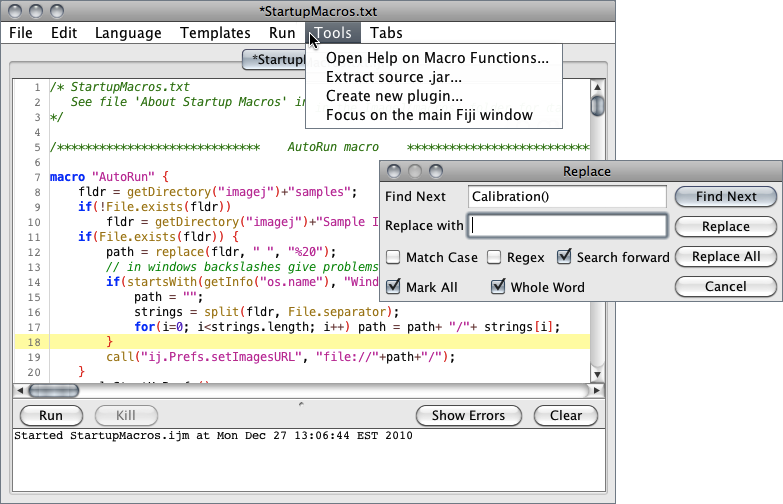
\includegraphics[scale=0.45]{images/FijiScriptEditor}\caption{\textbf{\label{fig:Fiji-Script-Editor}The Fiji Script Editor (ImageJA\ 1.44m).
}The Fiji Editor is an advanced text editor, supporting BeanShell,
Jython, JRuby and other scripting languages. It does not support \protect\userinterface{\nameref{FunctionFinder[F]}}
but selecting a built-in macro function and running \protect\userinterface{Tools\lyxarrow{}Open Help on Macro Functions\ldots{}}
retrieves the documentation for the selected function.}
\end{figure}



\calso{\noindent \nameref{sec:ScriptingOtherLang}, \nameref{sub:IJ-cmd-line},
\href{http://imagejdocu.tudor.lu/doku.php?id=plugin:utilities:ij_ed:start}{IJ\_{}ED},
a plugin by J�r�me Mutterer that binds \href{http://www.jedit.org/}{jEdit}
to ImageJ }


\section[Running ImageJ From the Command Line]{Running ImageJ from the Command Line\label{sub:IJ-cmd-line}}

ImageJ was devised as a desktop application. It can, however, run
without a graphics environment (\index{Headless mode}headless mode)
by adding a special library (\code{headless.jar}) to the \code{ij.jar}
classpath that overrides key ImageJ classes to work better headlessly.
As described on the \href{http://fiji.sc/wiki/index.php/Headless}{Fiji website},
this strategy is implemented in \nameref{sub:Fiji-intro} through
the \code{-}\code{-headless} command line flag (\emph{see also}
\href{http://imagejdocu.tudor.lu/doku.php?id=faq:technical:how_do_i_run_imagej_without_a_graphics_environment_headless}{Running ImageJ in headless mode}
and \href{http://cmci.embl.de/documents/100922imagej_cluster}{Using Cluster for Image Processing with IJ}).
Headless operations are simplified in \nameref{sub:ImageJ2intro}.

ImageJ recognizes the following command line options:

\begingroup
%change ttvariant to courier since default monospaced font does not allow bold typeface
\renewcommand{\ttdefault}{pcr}

\begin{lyxlist}{eval-macro-code-batch-pat}
\item [{\texttt{\textbf{\code{\noindent \texttt{\textbf{\textquotedbl{}file-name}}\texttt{\textquotedbl{}}}}}}] \noindent Opens
a file. Examples:\\
\texttt{\hspace*{15pt}\code{\noindent \texttt{blobs.tif}}}\\
\texttt{\hspace*{15pt}\code{\noindent \texttt{/Users/wayne/images/blobs.tif}}}\\
\texttt{\hspace*{15pt}\code{\noindent \texttt{e81{*}.tif}}}
\item [{\texttt{\textbf{-ijpath\ path}}}] \noindent Specifies the path
to the directory containing the plugins directory. Example:\\
\texttt{\hspace*{15pt}\code{\noindent \texttt{-ijpath /Applications/ImageJ}}}
\item [{\texttt{\textbf{-port}}}] \noindent Specifies the port ImageJ uses
to determine if another instance is running. Examples:\texttt{}~\\
\texttt{\hspace*{15pt}\code{\noindent \texttt{-port1}}} (use default
port address + 1) \\
\texttt{\hspace*{15pt}\code{\noindent \texttt{-port2}}} (use default
port address + 2)\\
\texttt{\hspace*{15pt}\code{\noindent \texttt{-port0}}} (do not
check for another instance (\href{http://imagej.nih.gov/ij/source/ij/OtherInstance.java}{OtherInstance})
\item [{\texttt{\textbf{-macro\ path\ {[}arg{]}}}}] \noindent Runs a
macro or script, passing it an optional argument, which can be retrieved
using \texttt{getArgument()}. Examples:\\
\texttt{\hspace*{15pt}\code{\noindent \texttt{-macro analyze.ijm}}}\\
\texttt{\hspace*{15pt}\code{\noindent \texttt{-macro analyze /Users/wayne/images/stack1} }}
\item [{\texttt{\textbf{-batch\ path\ {[}arg{]}}}}] \noindent Runs a
macro or script in batch mode (no GUI), passing it an optional argument.
ImageJ exits when the macro finishes.
\item [{\texttt{\textbf{-eval\ \textquotedbl{}macro\ code\textquotedbl{}}}}] \noindent Evaluates
macro code. Examples:\\
\texttt{\hspace*{15pt}\code{\noindent \texttt{-eval \textquotedbl{}print(\textquotesingle{}Hello,
world\textquotesingle{});\textquotedbl{}}}}\\
\texttt{\hspace*{15pt}\code{\noindent \texttt{-eval \textquotedbl{}return getVersion();\textquotedbl{}}}}
\item [{\texttt{\textbf{-run\ command}}}] \noindent Runs an ImageJ menu
command. Example:\\
\texttt{\hspace*{15pt}\code{\noindent \texttt{-run \textquotedbl{}About ImageJ\ldots{}\textquotedbl{}}}}
\item [{\texttt{\textbf{-debug}}}] \noindent Runs ImageJ in debug mode.
\end{lyxlist}
\endgroup


\calso{\href{http://imagej.nih.gov/ij/docs/install/linux.html}{Linux installation},
\href{http://imagejdocu.tudor.lu/doku.php?id=diverse:start&s[]=command&s[]=line}{ImageJ Documentation Portal: Command line}}
\clearpage{}

\thispagestyle{plain}
\sectionmark{The ImageJ Window}


\part{ImageJ User Interface\label{par:User-Interface1}}

Unlike most image processing programs ImageJ does not have a main
work area\nomenclature{GUI}{Graphical User Interface}. ImageJ's main
window is actually quite parsimonious containing only a menu bar (at
the top of the screen on the Mac) containing all the \nameref{par:Commands},
a \nameref{sub:Toolbar}, a \nameref{sub:Status-bar} and a \nameref{sub:Progress-bar}.
Images, histograms, profiles, widgets, etc.\ are displayed in additional
windows. Measurement results are displayed in the \nameref{sec:Results-Table}.
Most windows can be dragged around the screen and resized. 

\begin{figure}[h]
\noindent \begin{centering}
\caption[Main ImageJ window]{\textbf{\label{fig:The-ImageJ-window}The ImageJ window (version\,1.46j).}}
\vspace*{2pt}

\par\end{centering}

\noindent \begin{centering}
\setlength{\tabcolsep}{0pt}%
\begin{tabular}{>{\centering}p{6.45mm}>{\centering}p{6.45mm}>{\centering}p{6.45mm}>{\centering}p{6.45mm}>{\centering}p{6.45mm}>{\centering}p{6.45mm}>{\centering}p{6.45mm}>{\centering}p{6.45mm}>{\centering}p{6.45mm}>{\centering}p{6.45mm}>{\centering}p{6.45mm}>{\centering}p{6.45mm}>{\centering}p{6.45mm}>{\centering}p{6.45mm}>{\centering}p{6.45mm}>{\centering}p{6.45mm}>{\centering}p{6.45mm}>{\centering}p{6.45mm}>{\centering}p{6.45mm}>{\centering}p{6.45mm}>{\centering}p{6.45mm}}
{\small 1} & {\small 2} & {\small 3} & {\small 4} & {\small 5} & {\small 6} & {\small 7} & {\small 8} & {\small 9} & {\small 10} & {\small 11} & {\small 12} & {\small A} & {\small B} & {\small C} & {\small D} & {\small E} & {\small F} & {\small G} & {\small H} & {\small 13}\tabularnewline
\multicolumn{21}{c}{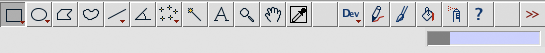
\includegraphics[width=136mm]{images/IJ_Window}}\tabularnewline
\noalign{\vskip-4.5pt}
\multicolumn{10}{l}{{\small \hspace*{15pt}\nameref{sub:Status-bar}}} & \multicolumn{11}{r}{{\small \nameref{sub:Progress-bar}\hspace*{15pt}}}\tabularnewline
\end{tabular}
\par\end{centering}

\noindent \begin{centering}
\vspace*{8pt}

\par\end{centering}

\noindent \centering{}\setlength{\tabcolsep}{0pt}~%
\begin{tabular}{>{\raggedright}m{6mm}>{\raggedright}p{72.5mm}>{\raggedright}p{9mm}>{\raggedright}p{49mm}}
{\small 1} & \multirow{2}{72.5mm}{{\small \nameref{sub:Rectangular-Selection-Tool} and \nameref{sub:Round-Rectangular-Selection}}} & {\small 8} & {\small \nameref{sub:Wand-Tool}}\tabularnewline
 &  & {\small 9} & {\small \nameref{sec:Text-Tool}}\tabularnewline
\noalign{\vskip\doublerulesep}
{\small 2} & \multirow{2}{72.5mm}{{\small \nameref{sub:Oval-Selection-Tool}, \nameref{sub:Elliptical-Selection-Tool}
and \nameref{sub:Brush-Selection-Tool} }} & {\small 10} & {\small \nameref{sec:Magnifying-Glass}}\tabularnewline
 &  & {\small 11} & {\small \nameref{sec:Scrolling-Tool}}\tabularnewline
\noalign{\vskip\doublerulesep}
{\small 3} & {\small \nameref{sub:Polygon-Selection-Tool}} & {\small 12} & {\small \nameref{sec:Color-Picker}}\tabularnewline
\noalign{\vskip\doublerulesep}
{\small 4} & {\small \nameref{sub:Freehand-Selection-Tool}} & {\small 13} & {\small \nameref{sec:ToolSwitcher}}\tabularnewline
\noalign{\vskip\doublerulesep}
{\small 5} & {\small \nameref{sub:Straight-Line-Selection}, \nameref{sub:Segmented-Line-Selection},
\nameref{sub:Freehand-Line-Selection} and \nameref{sec:Arrow-Tool} } & {\small A--H} & \multirow{3}{49mm}{Customized tools installed from \filenameref{StartupMacros.txt},
\dirnameref{macros/toolsets/}, \dirnameref{macros/tools/} or \dirnameref{plugins/Tools/} }\tabularnewline
\noalign{\vskip\doublerulesep}
{\small 6} & {\small \nameref{sec:Angle-Tool}} &  & \tabularnewline
\noalign{\vskip\doublerulesep}
{\small 7} & {\small \nameref{sec:Point-Tool} and \nameref{sec:Multi-point-Tool}} &  & \tabularnewline
\end{tabular}
\end{figure}



\subsection*{Toolbar\label{sub:Toolbar}}

The ImageJ toolbar contains tools for making selections, drawings,
zooming and scrolling, etc. In addition, the right-side of the toolbar
contains seven slots that can host any of the \href{http://imagej.nih.gov/ij/macros/tools/}{60+ tools}
and \href{http://imagej.nih.gov/ij/macros/toolsets/}{15+ toolsets}
available on the ImageJ website (\emph{see} \nameref{sec:CustomToolsAndToolsets}). 

All ImageJ \index{Toolbar}tools share common features:
\begin{itemize}
\item The\ 
\includegraphics{images/tools/triangle}\  on the bottom right
corner of some icons in the toolbar depicts a contextual menu that
can be accessed by right-clicking on the tool icon (e.g., \nameref{sub:StacksMenu}).
\item If an `Options' dialog is available for a particular tool, it can
be accessed by double clicking on the tool icon (e.g., \nameref{sub:Wand-Tool}).
\end{itemize}

\subsection*{Status bar\label{sub:Status-bar}}

When the cursor is over an image, pixel intensities and \index{Coordinates}coordinates
are displayed in the \index{Status bar}status bar. After running
a filter, elapsed time and processing rate (in pixels\,/\,second)
are also displayed. When clicking on the status bar the ImageJ version,
the Java version, \index{Memory}\index{RAM@RAM  \see{Memory,}}memory
in use, memory available and percent memory used will be displayed.
As \nameref{sec:Selections-Intro} are created or resized, selection
properties (e.g., location, width, etc.) are displayed on the status
bar.

\noindent In addition, clicking on ImageJ's status bar, forces the
Java garbage collector to run, which may help to reclaim unused memory
(\emph{see}\textsf{ \userinterface{\textsf{Edit\lyxarrow{}Options\lyxarrow{}\nameref{sub:Memory-&-Threads...}}}}).
You can assess this by running \textsf{\userinterface{\textsf{Plugins\lyxarrow{}Utilities\lyxarrow{}\nameref{sub:Monitor-Memory...}}}}:
each click on the Status bar should lead to a spike in the ImageJ's
memory utilization. 
\begin{figure}[H]
\noindent \centering{}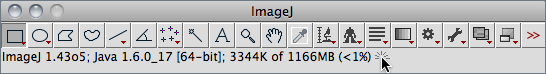
\includegraphics[scale=0.55]{images/StatusBar}
\end{figure}



\calso{\noindent \textsf{\userinterface{\textsf{Plugins\lyxarrow{}Utilities\lyxarrow{}\nameref{sub:ImageJ-Properties...}}},
\userinterface{\textsf{Help\lyxarrow{}\nameref{sub:About-ImageJ...}}}}}

\noindent {\small }
\begin{infobox}
\caption{\label{infobox:Toggle-Cal-Units}Toggling Calibrated Units}


\noindent If a spatial scale has been defined in \userinterface{\noindent Image\lyxarrow{}\nameref{sub:Image>Properties...}}
or \userinterface{\noindent Analyze\lyxarrow{}\nameref{sub:Set-Scale...}},
selection properties are displayed in the \nameref{sub:Status-bar}
in calibrated units. Resizing or moving while holding down \mykeystroke{\noindent Alt}
forces this information to be displayed in pixels.
\end{infobox}
{\small \par}


\subsection*{\noindent Progress bar\label{sub:Progress-bar}}

The \index{Progress bar}progress bar, located to the right of the
status bar, shows the progress of time-consuming operations. It will
not appear if the operation requires less then approximately one second.

%% Momentarily, do not show page numbers for sections in the TOC
\addtocontents{toc}{\protect\cftpagenumbersoff{section}}


\section{Tools\label{sec:IJ-Tools}}

%% Restore defaults
\addtocontents{toc}{\protect\cftpagenumberson{section}}

%% Adjust the lyxlist environment to accomodate the modifier key lists. We'll revert after this section
\renewenvironment{lyxlist}[1]{%
  \begin{list}{}{%
    \settowidth{\labelwidth}{#1}
    \addtolength{\labelwidth}{3.5ex}
    \addtolength{\topsep}{-1.2ex}
    \setlength{\leftmargin}{\labelwidth}
    \addtolength{\leftmargin}{\labelsep}
    \renewcommand{\makelabel}[1]{\qquad{}##1\hfil}
  }%
}{\end{list}}



\subsection{Area Selection Tools\label{sec:Area-selection-tools}}

These tools share the first four toolbar slots. As described in \nameref{sub:Toolbar},
use the right click drop-down menu to switch a different tool. Selection
Color can be changed by double clicking on the \nameref{sec:Point-Tool}/\nameref{sec:Multi-point-Tool}.


\subsubsection[Rectangular Selection Tool]{\noindent \textsf{\protect
\includegraphics[bb=0bp 5bp 20bp 20bp,scale=0.6]{images/tools/Rectangle}}~Rectangular
Selection Tool\label{sub:Rectangular-Selection-Tool}\index{Tools!Area Selection!Rectangle}\index{Rectangular selection}}

\noindent Location, width, height, and aspect ratio are displayed
in the status bar during drawing (\emph{see} \ref{infobox:Toggle-Cal-Units}
\nameref{infobox:Toggle-Cal-Units}).

Modifier keys:
\begin{lyxlist}{00.00.0000}
\item [{\mykeystroke{Shift}}] \noindent Selection is constrained to a
square
\item [{\mykeystroke{Alt}}] \noindent Current \index{Aspect ratio}aspect
ratio is maintained while resizing\\
With arrow keys, width and height are changed one pixel at a time
\item [{\mykeystroke{Ctrl}}] \noindent Selection is resized around the
center
\end{lyxlist}

\calso{\nameref{sub:Round-Rectangular-Selection}, \textsf{\nameref{sub:Specify...}},
\ref{infobox:Color} \nameref{infobox:Color}, \nameref{sub:Tools-shortcuts}}


\subsubsection[Rounded Rectangular Selection Tool]{\noindent \textsf{\protect
\includegraphics[bb=0bp 5bp 20bp 20bp,scale=0.6]{images/tools/RoundRect}}~Rounded
Rectangular Selection Tool\label{sub:Round-Rectangular-Selection}\index{Tools!Area Selection!Rounded Rectangle}\index{Rounded rectangle}\improvement{}}

\noindent %
\begin{minipage}[c][1\totalheight][t]{0.41\columnwidth}%
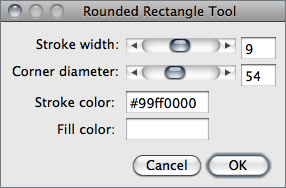
\includegraphics[scale=0.55]{images/RoundRectangle}%
\end{minipage}%
\begin{minipage}[c][1\totalheight][t]{0.59\columnwidth}%
This tool creates rectangular shapes with rounded corners. It shares
the same toolbar slot and the same modifier keys with the \nameref{sub:Rectangular-Selection-Tool}.
Double clicking on its icon opens the depicted dialog in which is
possible to specify:
\begin{description}
\item [{\emph{Stroke\ width}}] The width of the contour.
\item [{\emph{Corner\ diameter}}] The arc size at the vertices.\end{description}
%
\end{minipage}
\begin{description}
\item [{\emph{Stroke/Fill\ Color}}] The contour (stroke) color or the
filling color of the rounded rectangle. As explained in \userinterface{Edit\lyxarrow{}Selection\lyxarrow{}\nameref{sub:Properties...}},
selections can be either filled or contoured, but not both. The nine
default selection colors (\emph{black}, \emph{blue}, \emph{cyan},
\emph{green}, \emph{magenta}, \emph{orange}, \emph{red}, \emph{white},
\emph{yellow}) can be typed as text. Any other color must be typed
in hex notation (\emph{see} \ref{infobox:HEX} \nameref{infobox:HEX}). 
\end{description}

\calso{\nameref{sub:Rectangular-Selection-Tool}, \ref{infobox:Color} \nameref{infobox:Color},
\nameref{sub:Tools-shortcuts}}


\subsubsection[Oval Selection Tool]{\noindent \textsf{\protect
\includegraphics[bb=0bp 5bp 20bp 20bp,scale=0.6]{images/tools/Oval}}~Oval
Selection Tool\label{sub:Oval-Selection-Tool}\index{Tools!Area Selection!Oval}\index{Oval selection}}

\noindent Location, width, height, and aspect ratio are displayed
in the status bar during drawing (\emph{see} \ref{infobox:Toggle-Cal-Units}
\nameref{infobox:Toggle-Cal-Units}).

Modifier keys:
\begin{lyxlist}{00.00.0000}
\item [{\mykeystroke{Shift}}] Selection becomes circular
\item [{\mykeystroke{Alt}}] \noindent Current \index{Aspect ratio}aspect
ratio is maintained while resizing\\
With arrow keys, width and height are changed one pixel at a time
\item [{\mykeystroke{Ctrl}}] Selection is resized around the center
\end{lyxlist}

\calso{\nameref{sub:Elliptical-Selection-Tool}, \textsf{\nameref{sub:Specify...}},
\ref{infobox:Toggle-Cal-Units} \nameref{infobox:Toggle-Cal-Units},
\ref{infobox:Color} \nameref{infobox:Color}, \nameref{sub:Tools-shortcuts}}


\subsubsection[Elliptical Selection Tool]{\noindent \textsf{\protect
\includegraphics[bb=0bp 5bp 20bp 20bp,scale=0.6]{images/tools/Ellipse}}~Elliptical
Selection Tool\label{sub:Elliptical-Selection-Tool}\index{Tools!Area Selection!Ellipse}\index{Elliptical selection}\improvement{}}

Ellipse properties are adjusted by dragging the four handlers on its
antipodal points \cite{C-EllipseTool}. To rotate or resize, drag
the handlers on its major axis (transverse diameter). To adjust eccentricity,
drag the handlers on its minor axis (conjugate diameter). 


\calso{\nameref{sub:Oval-Selection-Tool}, \ref{infobox:Color} \nameref{infobox:Color},
\nameref{sub:Tools-shortcuts}}


\subsubsection[Brush Selection Tool]{\noindent \textsf{\protect
\includegraphics[bb=0bp 5bp 20bp 20bp,scale=0.6]{images/tools/Brush}}~Brush
Selection Tool\label{sub:Brush-Selection-Tool}\index{Tools!Area Selection!Brush}\index{Brush selection tool}\index{Selection!Refine}\improvement{}}

\noindent Adjusts (refines) the shape of area selections using a circular
`brush' \cite{C-ROIbrush}. Clicking inside the area selection and
dragging along its boundary will expand the boundary outwards. Clicking
outside the area selection and dragging along its boundary will shrink
the boundary inwards. Once the tool has been applied, ImageJ will
treat the adjusted ROIs as \nameref{sub:Composite-selections}. The
brush diameter can be adjusted by double clicking on the tool icon.

\noindent Modifier keys:
\begin{lyxlist}{00.00.0000}
\item [{\mykeystroke{Shift}}] \noindent Holding Shift forces the Brush
Selection Tool to add pixels to the selection
\item [{\mykeystroke{Alt}}] \noindent Holding Alt forces the Brush Selection
Tool to subtract pixels from the selection
\end{lyxlist}

\calso{\ref{infobox:Composites} \nameref{infobox:Composites}, \nameref{sub:Tools-shortcuts}}


\subsubsection[Polygon Selection Too\textsf{l}]{\noindent \textsf{\protect
\includegraphics[bb=0bp 5bp 20bp 20bp,scale=0.6]{images/tools/Polygon}}~Polygon
Selection Tool\textsf{\label{sub:Polygon-Selection-Tool}}\index{Tools!Area Selection!Polygon}\index{Polygon selection}}

Creates irregularly shaped selections defined by a series of line
segments. Segment length and angle are displayed in the status bar
during drawing (\emph{see} \ref{infobox:Toggle-Cal-Units} \nameref{infobox:Toggle-Cal-Units}).
To create a polygon selection, click repeatedly with the mouse to
create line segments. When finished, click in the small box at the
starting point (or double click), and ImageJ will automatically draw
the last segment. The vertex points that define a polygon selection
can be moved and modifier keys can be used to delete or add new vertexes
to the polygon. 

Modifier keys:
\begin{lyxlist}{00.00.0000}
\item [{\mykeystroke{Shift}}] \noindent Shift-clicking on an existing
vertex of the polygon adds a new corner point, smoothing the polygon
edge
\item [{\mykeystroke{Alt}}] \noindent Alt-clicking on an existing vertex
of the polygon removes it
\end{lyxlist}

\calso{\nameref{sub:Segmented-Line-Selection}, \userinterface{\textsf{\nameref{sub:Enlarge...}}},
\ref{infobox:Toggle-Cal-Units} \nameref{infobox:Toggle-Cal-Units},
\ref{infobox:Color} \nameref{infobox:Color}, \nameref{sub:Tools-shortcuts}}


\subsubsection[Freehand Selection Tool]{\noindent \textsf{\protect
\includegraphics[bb=0bp 5bp 20bp 20bp,scale=0.6]{images/tools/Freehand}}~Freehand
Selection Tool\label{sub:Freehand-Selection-Tool}\index{Tools!Area Selection!Freehand}\index{Freehand area selection}}

As with the polygon selection tool, ImageJ automatically draws the
last segment. Location and intensity of starting pixel are displayed
in the status bar during drawing.


\calso{\nameref{sub:Freehand-Line-Selection}, \nameref{sub:Polygon-Selection-Tool},
\textsf{\userinterface{\textsf{\nameref{sub:Enlarge...}}}}, \ref{infobox:Toggle-Cal-Units}
\nameref{infobox:Toggle-Cal-Units}, \ref{infobox:Color} \nameref{infobox:Color},
\nameref{sub:Tools-shortcuts}}


\subsection{Line Selection Tools\label{sec:Line-Selection-Tools}}

Use these tools to create line selections. The three line selection
tools share the same toolbar slot. As described in \nameref{sub:Toolbar},
use the right click drop-down menu to switch between line tools. 

Double click on any line tool to specify the line width by opening
the \textsf{\userinterface{\textsf{Image\lyxarrow{}Adjust\lyxarrow{}\nameref{sub:Line-WidthSlider}}}}
widget, on which is also possible to apply a cubic spline fit to a
polyline selection. Check the \emph{Sub-pixel resolution} checkbox
in \userinterface{Edit\lyxarrow{}Options\lyxarrow{}\nameref{sub:Profile-Plot-Options...}}
to create line selections with floating-point coordinates (\emph{see}
\nameref{sub:Sub-pixel-Selections}).


\subsubsection[Straight Line Selection Tool]{\protect
\includegraphics[bb=0bp 5bp 20bp 20bp,scale=0.6]{images/tools/StraightLine}~Straight
Line Selection Tool\label{sub:Straight-Line-Selection}}

\index{Tools!Line Selection!Straight Line}\index{Straight line selection}Length
and line angle are displayed in the status bar during drawing (\emph{see}
\ref{infobox:Toggle-Cal-Units} \nameref{infobox:Toggle-Cal-Units}). 

\noindent Modifier keys:
\begin{lyxlist}{00.00.0000}
\item [{\mykeystroke{Shift}}] \noindent Forces the line to be either horizontal
or vertical
\item [{\mykeystroke{Alt}}] \noindent Keeps the line length fixed while
moving either end of the line\\
Forces the two points that define the line to have integer coordinates
when creating a line on a zoomed image
\item [{\mykeystroke{Ctrl}}] \noindent While moving either end of the
line, the line is rotated/resized about its center
\end{lyxlist}

\calso{\textsf{\userinterface{\textsf{\nameref{sub:Calibration-Bar...}}}},
\textsf{\userinterface{\textsf{i\nameref{sub:Set-Scale...}}}}, \ref{infobox:Toggle-Cal-Units}
\nameref{infobox:Toggle-Cal-Units}, \ref{infobox:Color} \nameref{infobox:Color},
\nameref{sub:Tools-shortcuts}}


\subsubsection[Segmented Line Selection Tool]{\protect
\includegraphics[bb=0bp 5bp 20bp 20bp,scale=0.6]{images/tools/SegLine}~Segmented
Line Selection Tool\label{sub:Segmented-Line-Selection}\index{Tools!Line Selection!Segmented Line}\index{Segmented Line selection}\improvement{}}

Works exactly as described for the \nameref{sub:Polygon-Selection-Tool}:
Create a segmented line selection by repeatedly clicking with the
mouse. Each click will define a new line segment. Double click when
finished, or click in the small box at the starting point. The points
that define a segmented line selection can be moved or deleted, and
new points can be added. Length and line angle are displayed in the
status bar during drawing (\emph{see} \nameref{infobox:Toggle-Cal-Units}). 

Modifier keys:
\begin{lyxlist}{00.00.0000}
\item [{\mykeystroke{Shift}}] \noindent Shift-clicking on an existing
vertex adds a new one, adding a new segment to the segmented line
\item [{\mykeystroke{Alt}}] \noindent Alt-clicking on an existing vertex
of the segmented line removes it
\end{lyxlist}

\calso{\nameref{sub:Polygon-Selection-Tool}, \nameref{sub:Freehand-Selection-Tool},
\ref{infobox:Toggle-Cal-Units} \nameref{infobox:Toggle-Cal-Units},
\ref{infobox:Color} \nameref{infobox:Color}, \nameref{sub:Tools-shortcuts}}


\subsubsection[Freehand Line Selection Tool]{\protect
\includegraphics[bb=0bp 5bp 20bp 20bp,scale=0.6]{images/tools/FreehandLine}~Freehand
Line Selection Tool\label{sub:Freehand-Line-Selection}\index{Tools!Line Selection!Freehand Line}\index{Freehand line selection}\improvement{}}

Select this tool and drag with the mouse to create a freehand line
selection.


\calso{\nameref{sub:Freehand-Selection-Tool}, \nameref{sub:OverlayBrush},
\ref{infobox:Toggle-Cal-Units} \nameref{infobox:Toggle-Cal-Units},
\ref{infobox:Color} \nameref{infobox:Color}, \nameref{sub:Tools-shortcuts}}


\subsection[Arrow Tool]{\noindent \protect
\includegraphics[bb=0bp 5bp 20bp 20bp,scale=0.6]{images/tools/Arrow}~Arrow
Tool\label{sec:Arrow-Tool}\textmd{\index{Tools!Line Selection!Arrow}\index{Arrows}\index{Tools!Arrow}}}

\noindent This tool shares the same toolbar slot with the \nameref{sec:Line-Selection-Tools}
and can also be installed on a dedicated toolbar slot using the \nameref{sec:ToolSwitcher}
menu (\emph{see} \nameref{sub:ArrowTool2}). Double clicking on the
tool icon opens its \emph{Options} prompt \cite{C-ArrowTool}. 

\begin{minipage}[c][1\totalheight][t]{0.348\columnwidth}%
\vspace*{15pt}
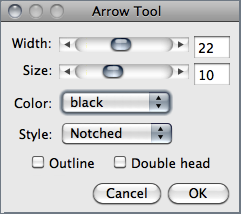
\includegraphics[scale=0.55]{images/ArrowTool}\vspace*{12pt}


\begin{spacing}{0.80000000000000004}
\noindent {\footnotesize }%
\begin{tabular}{>{\raggedright}b{7.8mm}c}
 & {\footnotesize Filled\,\,\ Notched\ \ \,Open}\tabularnewline
{\footnotesize Single head} & {\footnotesize 
\includegraphics[scale=0.65]{images/ArrowTypesS}}\tabularnewline
{\footnotesize Double head} & {\footnotesize 
\includegraphics[scale=0.65]{images/ArrowTypesD}}\tabularnewline
{\footnotesize Outline ~~~} & {\footnotesize 
\includegraphics[scale=0.65]{images/ArrowTypesO}}\tabularnewline
\end{tabular}\end{spacing}
%
\end{minipage}%
\begin{minipage}[c][1\totalheight][t]{0.652\columnwidth}%
Being an \index{Annotations}annotation tool, arrows are created using
foreground color (\emph{see} \textsf{\userinterface{\textsf{\nameref{sub:Color-Picker...[K]}}}})
and not selection color (\emph{see} \nameref{sec:Point-Tool}).

\medskip{}


\emph{Width} and \emph{Size} (in pixels) can be adjusted by dragging
the respective sliders or by direct input. Apart from the arrow styles
listed here, a \emph{Headless} option is also available. As for painting
tools (\nameref{sub:Brush}, \nameref{sub:FloodFiller} and \nameref{sub:Pencil}),
the \emph{Color} dropdown menu provides a convenient way to reset
the foreground color to one of the default options.\medskip{}


\noindent As with any other selection, add arrows to the non-destructive
overlay by pressing \mykeystroke{\noindent B} (\textsf{\userinterface{\noindent \textsf{Image\lyxarrow{}Overlay\lyxarrow{}\nameref{sub:Add-Selection...[b]}}}})
or \mykeystroke{\noindent D} (\textsf{\userinterface{\noindent \textsf{Edit\lyxarrow{}\nameref{sub:Draw-[d]}}}})
to permanently draw the arrow on the image (\emph{see} \ref{infobox:Color}
\nameref{infobox:Color} when working with non-RGB images).\medskip{}


\noindent The same modifier keys described to the \nameref{sub:Straight-Line-Selection}
apply to the arrow tool:%
\end{minipage}.
\begin{lyxlist}{00.00.0000}
\item [{\mykeystroke{Shift}}] \noindent Forces the line to be either horizontal
or vertical
\item [{\mykeystroke{Alt}}] \noindent Keeps the line length fixed while
moving either end of the line\\
Forces the two points that define the line to have integer coordinates
when creating a line on a zoomed image
\item [{\mykeystroke{Ctrl}}] \noindent While moving either end of the
line, the line is rotated/resized about its center
\end{lyxlist}

\calso{\nameref{fig:CPtool}, \ref{infobox:Color} \nameref{infobox:Color},
\nameref{sub:Brush}, \nameref{sub:OverlayBrush}, \nameref{sub:Pencil},
\nameref{sec:Text-Tool}, \nameref{sub:Tools-shortcuts}}


\subsection[Angle Tool]{\noindent \textsf{\protect
\includegraphics[bb=0bp 5bp 20bp 20bp,scale=0.6]{images/tools/Angle}}~Angle
Tool\label{sec:Angle-Tool}\index{Tools!Angle}\index{Angle tool}\index{Reflex angles}}

\sectionmark{Tools}

This tool allows you to measure an angle defined by three points.
Double click on the angle tool icon to enable the measurement of reflex
angles. The angle is displayed in the status bar while the selection
is being created or adjusted. Press \mykeystroke{M} (\textsf{\userinterface{\textsf{Analyze\lyxarrow{}\nameref{sub:Measure...[m]}}}})
to record the angle in the  \nameref{sec:Results-Table}.


\calso{\nameref{sub:Tools-shortcuts}}


\subsection[Point Tool]{\noindent \textsf{\protect
\includegraphics[bb=0bp 5bp 20bp 20bp,scale=0.6]{images/tools/Point}}~Point
Tool\label{sec:Point-Tool}\index{Tools!Point}\index{Point tool}\index{Counting objects}\improvement{}}

Use this tool to create a point selection, to count objects or to
record pixel \index{Coordinates}coordinates.

Modifier keys:
\begin{lyxlist}{00.00.0000}
\item [{\mykeystroke{Shift}}] \noindent Shift-clicking adds more points,
creating a multi-point selection (\emph{see} \nameref{sec:Multi-point-Tool}).
Point count is displayed on the \nameref{sub:Status-bar}
\item [{\mykeystroke{Alt}}] \noindent Alt-clicking on a point deletes
it. Alt-clicking and dragging with the \nameref{sub:Rectangular-Selection-Tool}
or \nameref{sub:Oval-Selection-Tool} deletes multiple points
\end{lyxlist}
\begin{minipage}[c][1\totalheight][t]{0.35\columnwidth}%
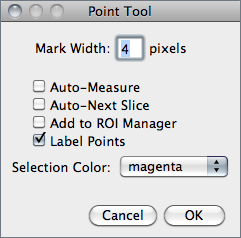
\includegraphics[scale=0.55]{images/PointOptions}%
\end{minipage}%
\begin{minipage}[c][1\totalheight][t]{0.65\columnwidth}%
Double clicking on the point tool icon (or running \textsf{\userinterface{\textsf{Edit\lyxarrow{}Options\lyxarrow{}\nameref{sub:Point-Tool...}}}})
displays its configuration dialog box.
\begin{description}
\item [{\emph{Mark\ Width}}] If greater than zero, a mark of the specified
diameter will be permanently drawn in the current foreground color
(cf.\ \textsf{\userinterface{\textsf{\nameref{sub:Color-Picker...[K]}}}}).
Note that marks modify the image (it may be wise to work with a copy)
and color marks are only available with RGB images (\emph{see} \ref{infobox:Color}
\nameref{infobox:Color}).\end{description}
%
\end{minipage}
\begin{description}
\item [{\emph{Auto-Measure}}] If checked, clicking on the image records
the pixel location and intensity. Note that if \emph{Mark Width} is
not zero, every time a point selection is measured a mark will be
painted (cf.\ \nameref{sub:Measure...[m]}). If unchecked, \userinterface{Edit\lyxarrow{}\nameref{sub:Draw-[d]}}
can be used to paint the mark (\emph{Mark Width }diameter) at the
location of each point.
\item [{\emph{Auto-Next\ Slice}}] If checked, ImageJ will automatically
advance to the next stack slice. Note that this feature will only
allow one point per slice. 
\item [{\emph{Add\ to\ ROI\ Manager}}] If checked, points will be automatically
added to the \nameref{sub:ROI-Manager...}
\item [{\emph{Label\ Points}}] \improvement{}If checked, each point selection
will be displayed with an accompanying numeric label.
\item [{\emph{Selection\ Color}}] Specifies \nameref{sec:Selections-Intro}
color, chosen from one of the nine default colors\emph{: red}, \emph{green},
\emph{blue}, \emph{magenta}, \emph{cyan}, \emph{yellow}, \emph{orange},
\emph{black} and \emph{white}. The chosen color is highlighted in
the center of the Point/MultiPoint Tool. It can also be specified
using \userinterface{Edit\lyxarrow{}Options\lyxarrow{}\nameref{sub:Colors...}}
\end{description}

\calso{\nameref{sec:Multi-point-Tool}, \nameref{lis:ChangeSelectionColor},
\index{Cell Counter plugin}\href{http://imagej.nih.gov/ij/plugins/cell-counter.html}{Cell Counter plugin},
\nameref{sub:Tools-shortcuts}}


\subsection[Multi-point Tool]{\noindent \textsf{\protect
\includegraphics[bb=0bp 5bp 20bp 20bp,scale=0.6]{images/tools/MultiPoint}}~Multi-point
Tool\label{sec:Multi-point-Tool}\index{Tools!Multi-point}\index{Multi-point tool}\index{Counting objects}\improvement{}}

The Multi-point Tool selects multiple points behaving as the \nameref{sec:Point-Tool}
when \mykeystroke{Shift} is pressed,\emph{ Label\ Points} is checked
and \emph{Auto-Measure} and \emph{Auto-Next\ Slice} are deselected.
As described for the \nameref{sec:Point-Tool}, \mykeystroke{Alt}
can also be used to remove points. Similarly, when using \textsf{\userinterface{\textsf{Edit\lyxarrow{}\nameref{sub:Draw-[d]}}}}
marks are painted with the diameter of \emph{Mark Width}. 


\calso{\nameref{sec:Point-Tool}, \index{Cell Counter plugin}\href{http://imagej.nih.gov/ij/plugins/cell-counter.html}{Cell Counter plugin},
\nameref{sub:Tools-shortcuts}}


\subsection[Wand Tool]{\noindent \textsf{\protect
\includegraphics[bb=0bp 5bp 20bp 20bp,scale=0.6]{images/tools/Wand}}~Wand
Tool\label{sub:Wand-Tool}\index{Tools!Area Selection!Wand}\index{Wand tool}\index{Tolerance (Wand Tool)}}

Creates a selection by \index{Tracing@Tracing \see{Wand tool,}}tracing
objects of uniform color or thresholded objects. To trace an object,
either click inside near the right edge, or outside to the left of
the object. To automatically outline and measure objects have a look,
e.g., at the \href{http://imagej.nih.gov/ij/macros/tools/WandAutoMeasureTool.txt}{WandAutoMeasureTool}
macro.

To visualize what happens, imagine a turtle that starts moving to
the right from where you click looking for an edge. Once it finds
the edge, it follows it until it returns to the starting point. Note
that the wand tool may not reliably trace some objects, especially
one pixel wide lines, unless they are thresholded (highlighted in
red) using \textsf{\userinterface{\textsf{Image\lyxarrow{}Adjust\lyxarrow{}\nameref{sub:Threshold...[T]}}}.}

Double clicking on the wand tool icon (or running \textsf{\userinterface{\textsf{Edit\lyxarrow{}Options\lyxarrow{}\nameref{sub:Wand-Tool...}}}})
opens the configuration dialog box in which three modes (4--connected,
8--connected or `Legacy') plus a tolerance value can be set \cite{C-WandTool}.
\begin{figure}[h]
\noindent 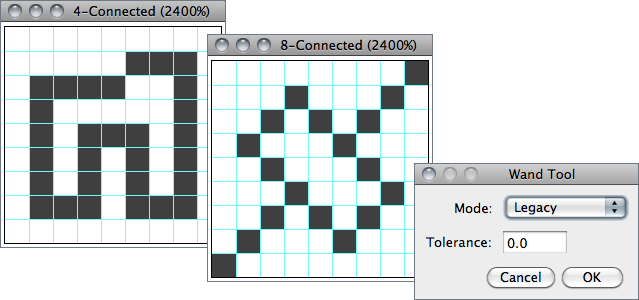
\includegraphics[scale=0.55]{images/WandTool}\caption{\textbf{The \nameref{sub:Wand-Tool}. }4/8--connected particles can
be traced within an intensity range.}
\end{figure}
\textbf{\emph{ }}\phantomsection{}
\begin{description}
\item [{\emph{\label{misc:WandTolerance}Tolerance}}] The wand takes the
pixel value where you click as an initial value. It then selects a
contiguous area under the condition that all pixel values in that
area must be in the range $initial\, value-tolerance$ to $initial\, value+tolerance$.\phantomsection{}
\item [{\emph{\label{misc:Wand4Connected}4--connected}}] Only the four
neighbors of a pixel are considered neighbors. E.g., the wand does
not follow a one-pixel wide diagonal line because the pixels of that
line are not four-connected.\phantomsection{}
\item [{\emph{\label{misc:Wand8Connected}8--connected}}] Each pixel is
considered to have eight neighbors. So the wand follows a diagonal
line if you click onto it. On the other hand, if you have an area
of constant value dissected by a one-pixel wide diagonal line, the
8--connected wand will `jump over the line' and include the other
part of that area.
\item [{\emph{Legacy}}] In this mode no neighbor is checked and no tolerance
is used. This is the default mode of the Wand Tool in ImageJ\,1.42
and earlier.
\end{description}
Modifier keys:
\begin{lyxlist}{00.00.0000}
\item [{\mykeystroke{Shift}}] \noindent Shift-clicking appends the traced
area to previously traced selections
\item [{\mykeystroke{Alt}}] \noindent Alt-clicking removes the traced
area from previously traced selections
\end{lyxlist}

\calso{\userinterface{Analyze\lyxarrow{}\nameref{sub:Analyze-Particles...}},
\nameref{sub:FloodFiller}, \href{http://imagejdocu.tudor.lu/doku.php?id=plugin:segmentation:versatile_wand:start}{Versatile Wand}
plugin, \nameref{sub:Composite-selections}, \nameref{sub:Tools-shortcuts}}


\subsection[Text Tool]{\noindent \textsf{\protect
\includegraphics[bb=0bp 5bp 20bp 20bp,scale=0.6]{images/tools/Text}}~Text
Tool\label{sec:Text-Tool}\index{Tools!Text}\index{Text}\index{Annotations}}

\begin{minipage}[c][1\totalheight][t]{0.3\columnwidth}%
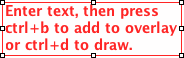
\includegraphics[scale=0.6]{images/TextTool}%
\end{minipage}%
\begin{minipage}[c][1\totalheight][t]{0.7\columnwidth}%
Use this tool to add text to images. It creates text ROIs, rectangular
selections containing one or more lines of text. Note the following
when using the Text Tool: %
\end{minipage}
\begin{itemize}
\item Font style and text alignment is specified in the \emph{Fonts} widget,
activated by double clicking on 
\includegraphics[bb=0bp 5bp 20bp 20bp,scale=0.6]{images/tools/Text}
or by running \userinterface{Edit\lyxarrow{}Options\lyxarrow{}\nameref{sub:Fonts...}}
Text is drawn in foreground color (\emph{see} \nameref{sub:Color-Picker...[K]})
\item Use the keyboard to add characters to the text and the backspace key
to delete characters. Use \mykeystroke{Alt} to type special unit
symbols such as $\micro$ (\mykeystroke{Alt}\mykeystroke{M}) or
$\angstrom$ (\mykeystroke{Alt}\mykeystroke{Shift}\mykeystroke{A}).
Note that menu shortcuts require holding down \mykeystroke{Ctrl}
while using the Text Tool (\emph{see} \nameref{sub:Using-Shortcuts})
\item Use \mykeystroke{Ctrl}\mykeystroke{Y} (\userinterface{Edit\lyxarrow{}Selection\lyxarrow{}\nameref{sub:Properties...}})
to re-adjust font color and size, text justification and to specify
a background color for the text selection. \ref{infobox:HEX} \nameref{infobox:HEX}
provides instructions on how to define semi-transparent colored backgrounds
(\emph{see also} \filenameref{\href{http://imagej.nih.gov/ij/macros/examples/DrawTextWithBackground.txt}{DrawTextWithBackground}}
macro)
\item Use \mykeystroke{Ctrl}\mykeystroke{B} (\userinterface{Image\lyxarrow{}Overlay\lyxarrow{}\nameref{sub:Add-Selection...[b]}})
to create non-destructive text annotations (\emph{see} \nameref{sub:Overlay-Intro};
\filenameref{\href{http://imagej.nih.gov/ij/macros/examples/OverlayDrawStringDemo.txt}{OverlayDrawStringDemo}},
\filenameref{\href{http://imagej.nih.gov/ij/macros/examples/TextOverlay.txt}{TextOverlay}}
macros). Alternatively, use \mykeystroke{Ctrl}\mykeystroke{D} (\userinterface{Edit\lyxarrow{}\nameref{sub:Draw-[d]}})
to permanently draw the text on the image. In the latter case, the
background of the text selection is not drawn (\emph{see also} \ref{infobox:Color}
\nameref{infobox:Color})
\end{itemize}

\calso{\nameref{sec:Arrow-Tool}, \nameref{sub:Brush}, \nameref{sub:OverlayBrush},
\nameref{sub:Pencil}, \filenameref{\href{http://imagej.nih.gov/ij/macros/TextDemo.txt}{TextDemo}}
macro, \nameref{sub:Tools-shortcuts} }


\subsection[Magnifying Glass]{\noindent \textsf{\protect
\includegraphics[bb=0bp 5bp 20bp 20bp,scale=0.6]{images/tools/Glass}}~Magnifying
Glass\label{sec:Magnifying-Glass}\index{Tools!Magnifying Glass}\index{Magnifying Glass Tool}}

Magnifies and reduces the view of the active image. Activate the tool
and click on the image to  \index{Zoom}zoom in. Right-click (or Alt-click)
to zoom out. The current magnification is shown in the image's title
bar. Double click on the magnifying glass icon to revert to the image's
original magnification. As explained in \textsf{\userinterface{Image\lyxarrow{}Zoom\lyxarrow{}\nameref{sub:ZoomIn}}},
there are 21 possible magnification levels: 3.1, 4.2, 6.3, 8.3, 12.5,
16.7, 25, 33.3, 50, 75, 100, 150, 200, 300, 400, 600, 800, 1200, 1600,
2400 and 3200\%. 

Modifier keys:
\begin{lyxlist}{00.00.0000}
\item [{\mykeystroke{Shift}}] \noindent Clicking and dragging while holding
down the Shift key runs \textsf{\userinterface{Image\lyxarrow{}Zoom\lyxarrow{}\nameref{sub:ZoomToSelection}}}
\item [{\mykeystroke{Alt}}] \noindent Image zooms out (right-click behavior)
\end{lyxlist}

\calso{\ref{infobox:ZoomedCanvas} \nameref{infobox:ZoomedCanvas}\textsf{,
\userinterface{\textsf{\nameref{sub:Zoom}}}} commands, \nameref{sub:Tools-shortcuts}}


\subsection[Scrolling Tool]{\noindent \textsf{\protect
\includegraphics[bb=0bp 5bp 20bp 20bp,scale=0.6]{images/tools/Hand}}~Scrolling
Tool\label{sec:Scrolling-Tool}\index{Tools!Scrolling}\index{Scrolling}}

Allows you to scroll through an image that is larger than its window.
You can temporarily activate this tool (except when using the \nameref{sec:Text-Tool})
by holding down the space bar.


\calso{\ref{infobox:ZoomedCanvas} \nameref{infobox:ZoomedCanvas}, \nameref{sub:Tools-shortcuts}}


\subsection[Color Picker Tool]{\noindent \textsf{\protect
\includegraphics[bb=0bp 5bp 20bp 20bp,scale=0.6]{images/tools/ColorPicker}}~Color
Picker\label{sec:Color-Picker}\index{Tools!Color Picker}\index{Color Picker}\index{Eye dropper}}

Sets the foreground drawing color by `picking up' colors from any
open image. Colors can also be picked up from the Color Picker (CP\nomenclature{CP}{Color Picker})
window (\textsf{\userinterface{\textsf{Image\lyxarrow{}Colors\lyxarrow{}}\nameref{sub:Color-Picker...[K]}}})
using any tool. In the icon, the `eye dropper' is drawn in the current
\index{Color!Foreground}foreground color while the frame around it
is drawn in the current \index{Color!Background}background color.
\userinterface{\textsf{Edit\lyxarrow{}}\nameref{sub:Draw-[d]}} and
\textsf{\userinterface{\textsf{Edit\lyxarrow{}}\nameref{sub:Fill-[f]}}}
use the foreground color. \textsf{\userinterface{\textsf{Edit\lyxarrow{}}\nameref{sub:Clear}}},
\userinterface{\nameref{sub:Clear-Outside}} and\textsf{ \userinterface{\textsf{\nameref{sub:Cut[x]}}}}
use the background color. Double clicking on the tool icon will display
the Color Picker window. 

Modifier key:
\begin{lyxlist}{00.00.0000}
\item [{\mykeystroke{Alt}}] \noindent Alt-clicking with the Color Picker
Tool on the image canvas `picks-up' background color 
\end{lyxlist}

\calso{\nameref{fig:CPtool}, \ref{infobox:Color} \nameref{infobox:Color},
\nameref{sub:Tools-shortcuts}, \nameref{lis:toolsShrtct3}}


\subsection[\emph{More Tools} Menu]{\noindent \textsf{\protect
\includegraphics[bb=0bp 5bp 20bp 20bp,scale=0.6]{images/tools/Switcher}}~\emph{More
Tools} Menu\label{sec:ToolSwitcher}\improvement{}\change{}}

The eight \nameref{sub:Toolbar} slots between the \nameref{sec:Color-Picker}
and the \emph{More Tools} Menu\index{Tools!More Tools Menu@\emph{More Tools} Menu}\index{More Tools Menu@\emph{More Tools} Menu}\index{Tools!Toolset Switcher@Toolset Switcher \see{\emph{More Tools} Menu,}}
can be customized using this drop-down menu (named \emph{Toolset Switcher}
in previous IJ versions). Tool configurations are stored in the ImageJ
preferences file (\emph{see} \nameref{sec:Settings-and-Preferences})
and retrieved across restarts. 

The \nameref{fig:MoreToolsList} is populated by \filenameref{\noindent StartupMacros.txt}
in \dirnameref{ImageJ/macros/}, \nameref{misc:Toolsets} installed
in \dirnameref{ImageJ/macros/toolsets/}, built-in tools loaded from
\filenameref{ij.jar} (\nameref{sub:ArrowTool2}, \nameref{sub:Brush},
\nameref{sub:DevMenu}, \nameref{sub:FloodFiller}, \nameref{sub:LUTMenu},
\nameref{sub:OverlayBrush}, \nameref{sub:Pencil}, \nameref{sub:SprayCan}
and \nameref{sub:StacksMenu}) and \nameref{misc:CustomSingleTools}
installed in \dirnameref{ImageJ/plugins/Tools/}.

At startup, the default set of tools is typically loaded from \index{StartupMacros}\filenameref{StartupMacros.txt}.
Later on, tools can be appended or replaced. \nameref{misc:CustomSingleTools}
are installed in the first available slot, or in the last slot if
no free slots are available\index{Toolsets}. \nameref{misc:Toolsets}
replace all the eight slots in the toolbar. Choose \emph{Remove Tool}s
to reset the toolbar. 

The icons for drawing tools installed from this menu reflect the foreground
color (\emph{see} \nameref{sub:Color-Picker...[K]}) and are updated
when the foreground color changes. 

Modifier key:
\begin{lyxlist}{00.00.0000}
\item [{\mykeystroke{Shift}}] \noindent Shift-clicking on the menu icon
will open the selected macro (\filenameref{.txt} and \filenameref{.ijm}
files)
\end{lyxlist}

\calso{\nameref{sec:CustomToolsAndToolsets}, \nameref{sub:Tools-shortcuts}}

\begin{figure}
\noindent {\small 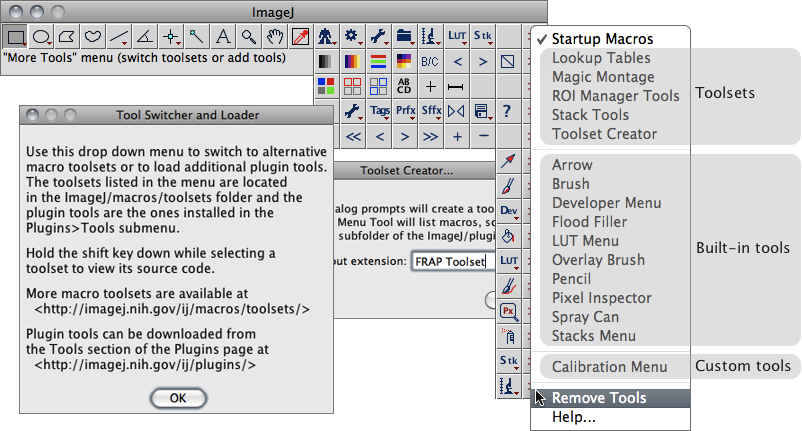
\includegraphics[scale=0.55]{images/MoreToolsMenu}}\caption[\emph{More Tools} list]{\label{fig:MoreToolsList}\textbf{\nameref{sec:ToolSwitcher} (IJ\,1.46n).}
The menu lists tools from \protect\filenameref{\noindent StartupMacros.txt}
in \protect\dirnameref{ImageJ/macros/}, \nameref{misc:Toolsets}
installed in \protect\dirnameref{ImageJ/macros/toolsets/}, built-in
tools loaded from \protect\filenameref{ij.jar} (\nameref{sub:ArrowTool2},
\nameref{sub:Brush}, \nameref{sub:DevMenu}, \nameref{sub:FloodFiller},
\nameref{sub:LUTMenu}, \nameref{sub:OverlayBrush}, \nameref{sub:Pencil},
\nameref{sub:SprayCan} and \nameref{sub:StacksMenu}) and \nameref{misc:CustomSingleTools}
installed in \protect\dirnameref{ImageJ/plugins/Tools/}. While toolsets
replace all the eight slots in the toolbar, single tools are installed
in the first available slot, or in the last slot if no free slots
are available.}
\end{figure}



\subsection[Arrow]{\noindent \textsf{\protect
\includegraphics[bb=0bp 5bp 20bp 20bp,scale=0.6]{images/tools/Switcher}}~\textsf{\protect
\includegraphics[bb=0bp 5bp 20bp 20bp,scale=0.6]{images/tools/Arrow2}}~Arrow\textmd{\index{Tools!Arrow}\index{Arrows}}\label{sub:ArrowTool2}\textmd{\index{Tools!Line Selection!Arrow}\index{Arrows}\index{Tools!Arrow}}\feature{}}

Installs a copy of the \nameref{sec:Arrow-Tool} on the first available
toolbar slot (or the last if no free slots are available), so that
it can be accessed without the need of selecting it on the \nameref{sec:Line-Selection-Tools}
dropdown menu. Refer to the original \nameref{sec:Arrow-Tool} for
details and modifier keys.


\calso{\nameref{fig:CPtool}, \ref{infobox:Color} \nameref{infobox:Color},
\nameref{sub:Brush}, \nameref{sub:OverlayBrush}, \nameref{sub:Pencil},
\nameref{sec:Text-Tool}, \nameref{sub:Tools-shortcuts}}


\subsection[Brush]{\noindent \textsf{\protect\includegraphics[bb=0bp 5bp 20bp 20bp,scale=0.6]{images/tools/Switcher}}~\textsf{\protect\includegraphics[bb=0bp 5bp 20bp 20bp,scale=0.6]{images/tools/Brush1}}~Brush\label{sub:Brush}\feature{New tools: Arrow, Brush, Developer Menu, Flood Filler, LUT Menu, Overlay Brush, Pencil, Pixel Inspector, Spray Can and Stacks Menu}}

\begin{minipage}[c][1\totalheight][t]{0.667\columnwidth}%
\includegraphics[scale=0.55]{images/Brush}%
\end{minipage}%
\begin{minipage}[c][1\totalheight][t]{0.333\columnwidth}%
A freehand \index{Brush}\index{Tools!Brush}\index{Paintbrush@Paintbrush \see{Brush and Overlay Brush,}}paintbrush
tool that draws invasively (as opposed to the \nameref{sub:OverlayBrush}
that draws on a non-destructive image overlay (\emph{see} \nameref{sub:Overlay-Intro}
and \userinterface{Image\lyxarrow{}\nameref{sub:Overlay}} commands).\medskip{}


Double clicking on the tool icon opens its \emph{Options} dialog box
in which is possible to specify the \emph{Brush width} (in pixels)
and \emph{Color}.%
\end{minipage}

Being an \index{Annotations}annotation tool, the paintbrush paints
in foreground color as reflected its icon (\emph{see} \ref{infobox:Color}
\nameref{infobox:Color} when working with non-RGB images). The \emph{Color}
dropdown menu provides a convenient way to reset the foreground color
to one of the default options, bypassing the need of opening the \nameref{fig:CPtool},
evoked using \mykeystroke{Ctrl} \mykeystroke{K}.\emph{ }As previously
described (\emph{see} \nameref{sec:Undo-and-Redo}), undo is restricted
to last drawing step. The Brush and \nameref{sub:Pencil} tools are
in all similar, differing only on brush (stroke) size.

Modifier keys:
\begin{lyxlist}{00.00.0000}
\item [{\mykeystroke{Shift}}] \noindent Shift-dragging on the canvas will
adjust the brush size
\item [{\mykeystroke{Alt}}] \noindent Holding Alt makes the brush paint
in background color 
\end{lyxlist}

\calso{\nameref{sub:OverlayBrush}, \nameref{sub:Pencil}, \nameref{sub:Freehand-Line-Selection},
\nameref{fig:CPtool}, \ref{infobox:Color} \nameref{infobox:Color},
\nameref{sub:Tools-shortcuts}}


\subsection[Developer Menu]{\noindent \textsf{\protect\includegraphics[bb=0bp 5bp 20bp 20bp,scale=0.6]{images/tools/Switcher}}~\textsf{\protect\includegraphics[bb=0bp 5bp 20bp 20bp,scale=0.6]{images/tools/DevMenu}}~Developer
Menu\label{sub:DevMenu}\index{Developer Menu}\index{Tools!Developer Menu}\feature{}}

A drop-down menu collecting several online resources and commands
that are useful when writing \nameref{sub:Macros-ExtendingIJ}, \nameref{sub:Plugins}
or troubleshooting ImageJ operations.

\emph{Debug mode} activates ImageJ's debugging mode (\userinterface{Edit\lyxarrow{}Options\lyxarrow{}\nameref{sub:Misc...}}).


\calso{\nameref{sec:Extending-ImageJ}, \nameref{sub:ImageJ-Macro-Editor},
\userinterface{\nameref{sec:Help}}, \userinterface{Plugins\lyxarrow{}\nameref{sub:Macros}}/\userinterface{\nameref{sub:Utilities}}/\userinterface{\nameref{sub:Plugins->New}},
\href{http://rsbweb.nih.gov/ij/plugins/cc-menu/index.html}{Common Commands Menu Tool},
\nameref{sub:StacksMenu}, \nameref{sub:LUTMenu}}


\subsection[Flood Filler]{\noindent \textsf{\protect\includegraphics[bb=0bp 5bp 20bp 20bp,scale=0.6]{images/tools/Switcher}}~\textsf{\protect\includegraphics[bb=0bp 5bp 20bp 20bp,scale=0.6]{images/tools/FloodFiller}}~Flood
Filler\label{sub:FloodFiller}\index{Flood Filler}\index{Tools!Flood Filler}\feature{}}

A \index{Paint Bucket Tool@Paint Bucket Tool \see{Flood Filler,}}\emph{paint
bucket }tool that fills with the current foreground color adjacent
pixels that have the same value as the clicked pixel. Double click
on the tool icon to specify the \href{http://en.wikipedia.org/wiki/Flood_fill}{flood type}
in terms of pixel connectivity: \nameref{misc:Wand4Connected} or
\nameref{misc:Wand8Connected}.

To spread the fill to contiguous pixels within an intensity range,
use the \nameref{sub:Wand-Tool} instead: Double click on the Wand
Tool icon to set a \nameref{misc:WandTolerance} value, then press
\mykeystroke{F} (\userinterface{Edit\lyxarrow{}\nameref{sub:Fill-[f]}})
to fill with foreground color (highlighted in the Flood Filler icon)
or \mykeystroke{Backspace}/\mykeystroke{Del} (\userinterface{Edit\lyxarrow{}\nameref{sub:Clear}})
to fill with background color (\emph{see} \userinterface{\nameref{sub:Color-Picker...[K]}}).

Modifier keys:
\begin{lyxlist}{00.00.0000}
\item [{\mykeystroke{Alt}}] \noindent Alt-clicking makes the brush paint
in background color
\end{lyxlist}

\calso{\code{\href{http://imagej.nih.gov/ij/developer/macro/functions.html\#floodFill}{floodFill(x,y)}}
macro function, \nameref{fig:CPtool}, \ref{infobox:Color} \nameref{infobox:Color},
\nameref{sub:Tools-shortcuts}}


\subsection[LUT Menu]{\noindent \textsf{\protect\includegraphics[bb=0bp 5bp 20bp 20bp,scale=0.6]{images/tools/Switcher}}~\textsf{\protect\includegraphics[bb=0bp 5bp 20bp 20bp,scale=0.6]{images/tools/LUTMenu}}~LUT
Menu\label{sub:LUTMenu}\index{LUT Menu}\index{Tools!LUT Menu}\feature{}}

A drop-down menu listing all the \userinterface{Image\lyxarrow{}\nameref{sub:Lookup-Tables}}
commands. It is a convenient way to deal with a large collection of
lookup tables that otherwise would only be accessed through the menu
bar. Note that although it is not possible to organize LUTs into subfolders,
it is possible to rename the most frequently used lookup tables with
a numeric prefix (e.g, \filenameref{\href{http://imagej.nih.gov/ij/download/luts/glasbey.lut}{01-glasbey.lut}},
\filenameref{\href{http://imagej.nih.gov/ij/download/luts/thermal.lut}{02-Termal.lut}},
etc.) so that they are listed earlier in the menu.


\calso{\nameref{sub:Pseudocolor-Images}, \filenameref{\href{http://imagej.nih.gov/ij/macros/Show_All_LUTs.txt}{Show\_{}All\_{}LUTs}}
(a macro that creates a \href{http://imagej.nih.gov/ij/download/luts/LUT_Montage.jpg}{graphical palette}
of all the installed lookup tables), \nameref{sub:StacksMenu}, \href{http://rsbweb.nih.gov/ij/plugins/cc-menu/index.html}{Common Commands Menu Tool},
\nameref{sub:DevMenu}}


\subsection[Overlay Brush]{\noindent \textsf{\protect\includegraphics[bb=0bp 5bp 20bp 20bp,scale=0.6]{images/tools/Switcher}}~\textsf{\protect\includegraphics[bb=0bp 5bp 20bp 20bp,scale=0.6]{images/tools/Brush2}}~Overlay
Brush\label{sub:OverlayBrush}\index{Overlay Brush}\index{Tools!Overlay Brush}\index{Annotations}\feature{}}

\begin{minipage}[c][1\totalheight][t]{0.645\columnwidth}%
\includegraphics[scale=0.55]{images/OverlayBrush}%
\end{minipage}%
\begin{minipage}[c][1\totalheight][t]{0.355\columnwidth}%
A freehand paintbrush that draws on a non-destructive image overlay
(\emph{see} \nameref{sub:Overlay-Intro}), as opposed to the \nameref{sub:Brush}
tool that draws invasively over the canvas.\medskip{}


Double clicking on the tool icon opens its \emph{Options} dialog box
in which is possible to specify the \emph{Brush width} (in pixels),
\emph{Transparency (\%)} and \emph{Color}.%
\end{minipage}

As previously described (\emph{see} \nameref{sub:Brush} and \nameref{sub:Pencil}
tools), the \emph{Color} dropdown menu changes the foreground color,
bypassing the \nameref{fig:CPtool} (activated by \mykeystroke{Ctrl}
\mykeystroke{K}). Press \emph{Undo} to remove the last painted stroke
from the overlay. Overlay manipulations are described in \userinterface{Image\lyxarrow{}\nameref{sub:Overlay}}.


\calso{\nameref{sub:Freehand-Line-Selection}, \ref{infobox:Color} \nameref{infobox:Color},
\nameref{sub:Tools-shortcuts}}


\subsection[Pencil]{\noindent \textsf{\protect\includegraphics[bb=0bp 5bp 20bp 20bp,scale=0.6]{images/tools/Switcher}}~\textsf{\protect\includegraphics[bb=0bp 5bp 20bp 20bp,scale=0.6]{images/tools/Pencil}}~Pencil\label{sub:Pencil}\index{Pencil}\index{Tools!Pencil}\feature{}}

A freehand painting tool that draws invasively in foreground color.
It is in all similar to the \nameref{sub:Brush} tool but it is typically
used with thinner strokes. Double clicking on the tool icon opens
its \emph{Options} dialog box in which is possible to specify the
\emph{Pencil width} (in pixels) and \emph{Color}. Refer to the \nameref{sub:Brush}
tool tools for details.

Modifier keys:
\begin{lyxlist}{00.00.0000}
\item [{\mykeystroke{Shift}}] \noindent Shift-dragging on the canvas will
adjust the brush size
\item [{\mykeystroke{Alt}}] \noindent Holding Alt makes the brush paint
in background color (\emph{see} \userinterface{\nameref{sub:Color-Picker...[K]}})
\end{lyxlist}

\calso{\nameref{sub:Freehand-Line-Selection}, \nameref{sub:OverlayBrush},
\nameref{fig:CPtool}, \ref{infobox:Color} \nameref{infobox:Color},
\nameref{sub:Tools-shortcuts}}


\subsection[Pixel Inspector]{\noindent \textsf{\protect\includegraphics[bb=0bp 5bp 20bp 20bp,scale=0.6]{images/tools/Switcher}}~\textsf{\protect\includegraphics[bb=0bp 5bp 20bp 20bp,scale=0.6]{images/tools/Inspector}}~Pixel
Inspector\textmd{\index{Tools!Pixel Inspector}\index{Pixel Inspector}}\label{sub:PixelInspector}\feature{}}

\begin{minipage}[c][1\totalheight][t]{0.605\columnwidth}%
\includegraphics[scale=0.55]{images/PixelInspector}%
\end{minipage}%
\begin{minipage}[c][1\totalheight][t]{0.395\columnwidth}%
The Pixel inspector displays the values of a square neighborhood around
the current cursor position as a table \cite{C-PixelInspector}. Values
are updated in real time as the mouse is dragged over the image. It
is useful to examine how a filter changes the pixel data. E.g., load
Pixel Inspector, move the cursor over an image and run \userinterface{Process\lyxarrow{}Filters\lyxarrow{}\nameref{sub:Gaussian-Blur...}}:
When toggling the \emph{Preview} checkbox you will be able to monitor
in real time how different \emph{Sigma} radius change pixel values.%
\end{minipage}

In the \emph{Pixel Values} table, columns and row headers (x \& y
positions) are expressed in pixel coordinates. The y-axis direction
is determined by the \nameref{misc:InvertYcoordinates} value in \userinterface{Analyze\lyxarrow{}\nameref{sub:Set-Measurements...}}
The center position (current cursor) is printed in red (\emph{x},
\emph{y}, \emph{value}). When the table is in the foreground, the
arrow keys can be used to nudge the neighborhood square (outlined
in red) and the table can be copied into the clipboard by pressing
\mykeystroke{C}. For settings, press the \emph{Prefs} button at the
top left of the table:
\begin{description}
\item [{\emph{Radius}}] Specifies the size of the table, $3\times3$ for
$radius=1$;  $5\times5$ for $radius=2$, etc. 
\item [{\emph{Grayscale\ readout}}] The numeric output for 8 and 16--bit
grayscale images. Can be\emph{ Raw} {[}the default{]}, \emph{Calibrated}
{[}\emph{see} \userinterface{Analyze\lyxarrow{}\nameref{sub:Calibrate...}}{]}
or Hexadecimal (\emph{Hex}).
\item [{\emph{RGB\ readout}}] The numeric output for RGB images. Can be
\emph{R,G,B} triplets, \emph{Gray Value} or Hexadecimal (\emph{Hex})
{[}\emph{see} \ref{infobox:HEX} \nameref{infobox:HEX}{]}. The mean
grayscale value is determined by the weighting factors specified in
\userinterface{Edit\lyxarrow{}Options\lyxarrow{}\nameref{sub:Conversions...}}
\item [{\emph{Copy\ to\ clipboard}}] Specifies which data is copied to
the clipboard. Choose \emph{Data only} to copy the table without headers,
\emph{x,y and Data} to copy the current position (x,y) values followed
by remaining data or \emph{Header and Data} to copy the table with
headers. Tables are copied as tab-delimited values.
\end{description}

\calso{\nameref{fig:TextImages}, \userinterface{Image\lyxarrow{}Transform\lyxarrow{}\nameref{sub:ImageToResults}/\nameref{sub:ResultsToImage}},
\userinterface{File\lyxarrow{}Save As\lyxarrow{}\nameref{sub:SaveAs>Text-Image...}},
\userinterface{Import\lyxarrow{}\nameref{sub:Import>Text-Image}},
\nameref{sub:Tools-shortcuts}}


\subsection[Spray Can]{\noindent \textsf{\protect\includegraphics[bb=0bp 5bp 20bp 20bp,scale=0.6]{images/tools/Switcher}}~\textsf{\protect\includegraphics[bb=0bp 5bp 20bp 20bp,scale=0.6]{images/tools/SprayCan}}~Spray
Can\label{sub:SprayCan}\feature{}}

The \index{Tools!Spray Can}\index{Spray Can}\index{Noise}Spray
Can (\emph{Airbrush} tool) draws random pixels in the current foreground
color (\emph{paint}) (\emph{see} \nameref{sub:Color-Picker...[K]}
and \ref{infobox:Color} \nameref{infobox:Color}). It behaves as
a traditional airbrush or spray paint: Holding the main mouse button
(without moving the cursor) will build up \emph{paint}, as if pressing
the nozzle of an aerosol paint can.\emph{ Spray widt}h,\emph{ Dot
size} and \emph{Flow rat}e can be specified by double clicking on
the tool icon.

This tool is useful to generate random spot noise. Use it to, e.g.,
assess the effectiveness of median filtering: Load the Spray Can tool,
apply it over an image and toggle the \emph{Preview} option in the
\userinterface{Process\lyxarrow{}Filters\lyxarrow{}\nameref{sub:Median...}}
prompt. 


\calso{\userinterface{Process\lyxarrow{}Noise\lyxarrow{}\nameref{sub:Add-Noise}},
\userinterface{\nameref{sub:Salt-and-Pepper}}, \nameref{sub:Tools-shortcuts}}


\subsection[Stacks Menu]{\noindent \textsf{\protect\includegraphics[bb=0bp 5bp 20bp 20bp,scale=0.6]{images/tools/Switcher}}~\textsf{\protect\includegraphics[bb=0bp 5bp 20bp 20bp,scale=0.6]{images/tools/StacksMenu}}~Stacks
Menu\label{sub:StacksMenu}\index{Stacks Menu}\index{Tools!Stacks Menu}\feature{}}

A drop-down menu collecting several commands related to \nameref{sub:Stacks-Intro}
and \nameref{sub:Hyperstacks-Intro}, otherwise accessed through the
hierarchy of \userinterface{Image\lyxarrow{}\nameref{sub:Stacks}},
\userinterface{Image\lyxarrow{}\nameref{sub:Hyperstacks}} and \userinterface{File\lyxarrow{}\nameref{sub:OpenSamples}}submenus.
The list makes a particular emphasis on commands that have no keyboard
shortcuts assigned.


\calso{\userinterface{Plugins\lyxarrow{}\nameref{sub:Shortcuts}}, \nameref{sub:LUTMenu},
\nameref{sub:StacksMenu}, \href{http://rsbweb.nih.gov/ij/plugins/cc-menu/index.html}{Common Commands Menu Tool},
\nameref{sub:DevMenu}}

%% Restore the lyxlist environment to its defaults
\renewenvironment{lyxlist}[1]{%
  \begin{list}{}{%
    \settowidth{\labelwidth}{#1}
    \setlength{\leftmargin}{\labelwidth}
    \addtolength{\leftmargin}{\labelsep}
    \renewcommand{\makelabel}[1]{##1\hfil}
  }%
}{\end{list}}



\section{\noindent Custom Tools\index{Tools!Custom tools}\index{Macro tools}\index{Plugin tools}\label{sec:CustomToolsAndToolsets}}

Customized tools are add-ons (macros and plugins) that allow custom
interactions with the ImageJ toolbar and/or the image canvas. They
are installed on the right side of the \nameref{sub:Toolbar} between
the \nameref{sec:Color-Picker} and the \nameref{sec:ToolSwitcher}.
At startup, the default set of tools is loaded from \index{StartupMacros}\filenameref{ImageJ/macros/StartupMacros.txt}.
Later on, tools can be appended or replaced using the \nameref{sec:ToolSwitcher}
menu. As mentioned, custom tool configurations are saved in the preferences
file, and thus remembered across restarts (\emph{see} \nameref{sec:Settings-and-Preferences}).

It is worth it to mention some differences between the installation
of single tools and toolsets:
\begin{description}
\item [{Single\ Tools\label{misc:CustomSingleTools}}] \index{Tools!Plugin Tools}\index{Plugin Tools}
Single tools are appended to the first available toolbar slot or installed
in the last slot if no free slots are available. Tools can be macros
(\filenameref{.txt} and \filenameref{.ijm} files) or \feature{Plugin Tools} \negthinspace{}\negthinspace{}plugins
(\filenameref{.class} and \filenameref{.jar} files) and are listed
on the \nameref{sec:ToolSwitcher} menu if placed in the \dirnameref{ImageJ/plugins/Tools/}
directory. In addition to the macro tools distributed with ImageJ
and saved in \dirnameref{ImageJ/macros/tools/}, a vast repertoire
of \href{http://imagej.nih.gov/ij/plugins/index.html\#tools}{tools}
is available on the ImageJ website.
\item [{Toolsets\label{misc:Toolsets}}] \index{Toolsets}Toolsets are
macro files (\filenameref{.txt} and \filenameref{.ijm} files) containing
up to eight macro tools, along with any number of ordinary macros.
Toolsets are listed on the \nameref{sec:ToolSwitcher} menu if installed
in the \dirnameref{ImageJ/macros/toolsets/} directory. Choosing a
toolset (e.g., \emph{Lookup Tables}) replaces all previously installed
tools. \\
As mentioned, \index{StartupMacros}\filenameref{ImageJ/macros/StartupMacros.txt}
contains the tools loaded at startup. This file can be customized
using \userinterface{Plugins\lyxarrow{}Macros\lyxarrow{}\nameref{sub:Startup-Macros...}}
or by holding \mykeystroke{Shift} when choosing \emph{Startup Macros}
from the \nameref{sec:ToolSwitcher} menu. \\
ImageJ feature several pre-installed toolsets \cite{C-Toolsets} and
many others are available on the \href{http://imagej.nih.gov/ij/plugins/index.html\#toolsets}{ImageJ website}.
Toolsets can also be created by choosing \emph{Toolset Creator}, a
convenient way to create groups of Menu Tools listing \userinterface{\nameref{sec:Plugins}}
commands.
\end{description}

\calso{\nameref{sec:ToolSwitcher}, \href{http://imagej.nih.gov/ij/developer/macro/macros.html\#tools}{Tools documentation},
\userinterface{Plugins\lyxarrow{}New\lyxarrow{}\nameref{sub:NewMacroTool}},
\userinterface{\nameref{sub:NewPluginTool}}}


\section[Contextual Menu]{Contextual Menu\label{sec:ContextualMenu}}

\begin{minipage}[c][1\totalheight][t]{0.413\columnwidth}%
\includegraphics[scale=0.55]{images/PopupMenu}%
\end{minipage}%
\begin{minipage}[c][1\totalheight][t]{0.587\columnwidth}%
As mentioned earlier macros and macro tools in the\texttt{ }\index{StartupMacros}\filenameref{StartupMacros.txt}
are automatically installed in the \textsf{\userinterface{\textsf{Plugins\lyxarrow{}Macros\lyxarrow{}}}
}submenu and in the toolbar when ImageJ starts up. 

\medskip{}
In addition, the \filenameref{StartupMacros.txt} file also installs
the \index{Contextual Menu}contextual (\index{Pop-up menu@Pop-up menu  \see{Contextual menu,}}popup)
menu displayed when right-clicking on an image. Other macros and toolsets
(e.g., \href{http://imagejdocu.tudor.lu/doku.php?id=howto:working:work_with_magic_montage}{Magic Montage})
may also replace the default menu with specialized ones. In this case,
re-installing the StartupMacros (using the \nameref{sec:ToolSwitcher})
will revert the contextual menu to its default.\medskip{}


\emph{\href{http://imagej.nih.gov/ij/docs/macro_reference_guide.pdf}{The ImageJ Macro Language --- Programmer's Reference Guide}}
explains how this menu can be customized: %
\end{minipage}
\begin{quotation}
The menu that is displayed when a user right-clicks (or ctrl-clicks)
on an image window can be customized through installation of the \texttt{\textquotedbl{}Popup
Menu\textquotedbl{}} macro. Any menu has a name and a list of menu
items. The \texttt{\code{\texttt{newMenu(name, items)}}} macro function
allows the creation of a new menu. This menu passes the chosen item
as a simple string to the \texttt{\code{\texttt{\textquotedbl{}Popup Menu\textquotedbl{}}}}
macro. From this point you can decide what to do, according to what
item was chosen.
\end{quotation}
\begin{lstlisting}[caption={Customizing the Image Popup Menu},label={lis:macro:PopupMenu},showstringspaces=false,tabsize=4]
 /* The "Popup Menu" macro defines the menu that is displayed when right clicking (or ctrl-clicking) on an image. It is part of the startup macros (StartupMacros.txt) and several other macro toolsets
 */
 var pmCmds= newMenu("Popup Menu", newArray("Help...", "Rename...", "Duplicate...", "Original Scale", "Paste Control...", "-", "Record...", "Capture Screen ", "Monitor Memory...", "Startup Macros...", "Search...", "-", "Find Maxima..."));

 macro "Popup Menu" {
  cmd= getArgument(); 
  if (cmd=="Help...")
     showMessage("About Popup Menu",
            "To customize this menu, edit the line that starts with\n"+
            "\"var pmCmds\" in ImageJ/macros/StartupMacros.txt.");
  else
     run(cmd);
 }
\end{lstlisting}


So, e.g., to add the ability to run the \textsf{\userinterface{\textsf{Process\lyxarrow{}\nameref{sub:Subtract-Background...}}}}
command from the contextual menu one can simply add that command to
the list of items defining the \texttt{\code{\texttt{PopUp Menu}}}.
Note that ``-'' defines menu separators:

\begin{lstlisting}[firstnumber=3,showstringspaces=false,tabsize=4]
 var pmCmds= newMenu("Popup Menu", newArray("Help...", "Rename...", "Duplicate...", "Original Scale", "Paste Control...", "-", "Record...", "Capture Screen ", "Monitor Memory...", "Startup Macros...", "Search...", "-", "Find Maxima...", "-", "Subtract Background..."));
\end{lstlisting}



\section{Results Table\label{sec:Results-Table}}

\noindent {\small Most of ImageJ analyses are printed to the \index{Results table@{\small Results table}}Results
table. Table commands} are organized in four menus:\textsf{\emph{\small{}
}}\textsf{\small File}\lyxarrow{}\emph{, }\textsf{\small Edit}\lyxarrow{}\emph{,
}\textsf{\small Font}\lyxarrow{}\emph{ }and\emph{ }\textsf{\small Results}\lyxarrow{}\emph{.
}A contextual menu listing the majority of these commands can be accessed
by right-clicking anywhere in the Results window.
\begin{description}
\item [{\textsf{\small File}\emph{\lyxarrow{}}\textsf{\small Save\ As\ldots{}}}] Exports
the measurements as a tab-delimited or comma-delimited text file as
defined in \textsf{\small Results}\emph{\lyxarrow{}}\textsf{\small Options\ldots{}}{\small \par}
\item [{\textsf{\small File}\emph{\lyxarrow{}}\textsf{\small Rename\ldots{}}}] Renames
the table. Because ImageJ outputs measurements exclusively to the
\emph{Results} table, renaming the table will freeze its contents.
\item [{\textsf{\small File}\emph{\lyxarrow{}}\textsf{\small Duplicate\ldots{}}}] Creates
a new table containing a copy of the data. Note that ImageJ will not
output measurements to duplicated tables.
\item [{\textsf{\small Font}\emph{\lyxarrow{}}}] This menu contains commands
to adjust font size.
\item [{\textsf{\small Results}\emph{\lyxarrow{}}\textsf{\small Clear\ Results\ldots{}}}] Alias
for the \userinterface{\nameref{sec:Analyze-Menu}\nameref{sub:Clear-Results}}
command.
\item [{\textsf{\small Results}\emph{\lyxarrow{}}\textsf{\small Summarize}}] Alias
for the \userinterface{\nameref{sec:Analyze-Menu}\nameref{sub:Summarize}}
command.
\item [{\textsf{\small Results}\emph{\lyxarrow{}}\textsf{\small Distribution\ldots{}}}] Alias
for the \userinterface{\nameref{sec:Analyze-Menu}\nameref{sub:Distribution...}}
command.
\item [{\textsf{\small Results}\emph{\lyxarrow{}}\textsf{\small Set\ Measurements\ldots{}}}] Alias
for the \userinterface{\nameref{sec:Analyze-Menu}\nameref{sub:Set-Measurements...}}
command.
\item [{\textsf{\small Results}\emph{\lyxarrow{}}\textsf{\small Options\ldots{}}}] Opens
the \userinterface{Edit\emph{\lyxarrow{}}Options\emph{\lyxarrow{}}\nameref{sub:Input/Output...}}
dialog in which is possible to specify if column headers and row numbers
should be saved or copied from ImageJ tables (including the Summarize
table, cf.\ \userinterface{Analyze\emph{\lyxarrow{}}\nameref{sub:Analyze-Particles...}}).
In addition, it allows to specify the file extension to be used when
saving data. Custom extensions (e.g., \filenameref{.csv}, \filenameref{.xls}
or \filenameref{.ods}) allow ImageJ tables to be imported seamlessly
by spreadsheet applications. ImageJ tables are saved in \index{CSV}CSV
format if \emph{File extension for tables} is \filenameref{.csv}.
\end{description}

\calso{\textsf{\userinterface{\textsf{\nameref{sec:Plugins}\nameref{sub:Plugins->New}\nameref{sub:Table...}}}}}

\noindent 
\begin{figure}
\noindent {\small \includegraphics[width=1\columnwidth]{images/ResultsTable}}{\small \par}

\noindent \caption{\textbf{ImageJ Results table (version\,1.44k).} Columns width can
be adjusted by clicking on and dragging the vertical lines that separate
the column headings. Selected rows can be deleted by pressing the
backspace key. The arrow keys can be used to vertically scroll the
window.}
\end{figure}



\section{Editor\label{sub:ImageJ-Macro-Editor}}

\nameref{sub:Macros}, \nameref{sub:Scripts} and \nameref{sub:Plugins}
can be opened and executed in the ImageJ editor. The \index{Editor}editor
commands are organized in five menus:\textsf{\emph{ }}\textsf{File}\emph{\lyxarrow{}\negthinspace{},}\textsf{
Edit}\emph{\lyxarrow{}\negthinspace{},}\textsf{ Font}\emph{\lyxarrow{}\negthinspace{},}\textsf{
Macros}\emph{\lyxarrow{}} and\textsf{ Debug}\emph{\lyxarrow{}.}
\begin{figure}[h]
\noindent \includegraphics[scale=0.55]{images/MacroEnvironment}\caption{\textbf{The ImageJ editor (version\,1.43n).} The editor is a simple
text editor featuring \nameref{FunctionFinder[F]}, an essential tool
when writing \nameref{sub:Macros-ExtendingIJ}. The \nameref{sub:Fiji-Scrip-Editor}
is a more advanced editor featuring syntax highlight and\textbf{ }support
to all of \nameref{sub:Fiji-intro}'s scripting languages.}
\end{figure}

\begin{description}
\item [{\textsf{File}\emph{\lyxarrow{}}}] Basic file operations (Open,
Save, Print, etc.) are listed in this menu. The last saving directory
is kept in \filenameref{IJ\_prefs.txt}, the IJ preferences file (\emph{see}
\nameref{sec:Settings-and-Preferences}).
\item [{\textsf{Edit}\emph{\lyxarrow{}}}] Similarly to any other text
editor this menu contains commands related to text handling as well
as commands for locating text. Specially useful are:

\begin{description}
\item [{\textsf{Go\ to\ Line\ldots{}\ {[}l{]}}}] \mykeystroke{Ctrl}\,\mykeystroke{L},
This dialog box enables you to quickly go to a specified line of code.
\item [{\textsf{Zap\ Gremlins}}] This command finds and deletes the extraneous
non-visible, non-printing characters that sometimes appear when cutting
and pasting from other sources, such as email messages that may contain
extraneous control characters, or any non-ASCII characters.
\item [{\textsf{Copy\ to\ Image\ Info}}] This command will copy the
selected text (or the entire contents of the editor if no selection
is present) to the image header, being available through the \textsf{\userinterface{Image\lyxarrow{}\nameref{sub:Show-Info...}}}
command. Note that the copied text will substitute any other information
present in the file header and will only be available in images saved
as TIFF (\emph{see} \ref{infobox:Formats} \nameref{infobox:Formats}).
\end{description}
\item [{\textsf{Font}\emph{\lyxarrow{}}}] This menu contains commands
to adjust font size and type. 
\item [{\textsf{Macros}\emph{\lyxarrow{}}}] This menu contains commands
that allow you to run, install or evaluate macro code:

\begin{description}
\item [{\textsf{Run\ Macro\ {[}r{]}}}] \mykeystroke{Ctrl}\,\mykeystroke{R},
Runs the macro or the selected line(s) of code.
\item [{\textsf{Evaluate\ Line\ {[}y{]}}}] \mykeystroke{Ctrl}\,\mykeystroke{Y},
Runs the line of code that contains the insertion point.
\item [{\textsf{Abort\ Macro}}] Exits the macro.
\item [{\textsf{Install\ Macros\ {[}i{]}}}] \mykeystroke{Ctrl}\,\mykeystroke{\,I},
Adds the macro(s) contained in the editor to \textsf{\userinterface{Plugins\lyxarrow{}\nameref{sub:Macros}}}
submenu (\textsf{\userinterface{\textsf{Plugins\lyxarrow{}Help\lyxarrow{}}\nameref{sub:Macro-Functions...}}}
command).
\item [{\textsf{Macro\ Functions\ldots{}\ {[}M{]}}}] \mykeystroke{Ctrl}\,\mykeystroke{Shift}\,\mykeystroke{\,M},
Opens the \index{Macro functions}\href{http://imagej.nih.gov/ij/developer/macro/functions.html}{Macro Functions reference page},
the indispensable guide to the built-in functions that can be called
from the ImageJ macro language (alias for \textsf{\userinterface{Help\lyxarrow{}\nameref{sub:Macro-Functions...}}).}\phantomsection{}
\item [{\textsf{\label{FunctionFinder[F]}Function\ Finder\ldots{}\ {[}F{]}}}] \mykeystroke{Ctrl}\,\mykeystroke{Shift}\,\mykeystroke{F},
\cite{C-FxFinder} Retrieves \index{Macro functions}macro functions
in the same way \nameref{sub:Command-Finder} retrieves commands.
Functions are read from the \filenameref{functions.html} file stored
in the macros folder (a local copy of \url{http://imagej.nih.gov/ij/developer/macro/functions.html}).
This file is deleted by \textsf{\userinterface{\textsf{Help\lyxarrow{}}\nameref{sub:Update-ImageJ...}}}
command every time ImageJ is updated to a release version (i.e., not
a \emph{daily build}, \emph{see} \nameref{sec:Updating-ImageJ}),
forcing Function Finder to download a fresh copy the next time it
is launched.\phantomsection{}
\item [{\textsf{\label{misc:EvaluateJavaScript}Evaluate\ JavaScript\ {[}j{]}}}] \mykeystroke{Ctrl}\,\mykeystroke{J},
Runs JavaScript code in the editor window. Note that \textsf{Run Macro
}runs JavaScript code if the title of the file ends with `.js'.
\end{description}
\item [{\textsf{Debug}\emph{\lyxarrow{}}}] This menu contains seven commands
related to the macro \index{Debug}debugging. You can debug a macro
using the commands in the \textsf{Debug} menu. You start a debugging
session initiating \textsf{\userinterface{Debug Macro}}. You can
then single step through the macro code by repeatedly running \textsf{\userinterface{Step}}. 

\begin{description}
\item [{\textsf{Debug\ Macro\ {[}d{]}}}] \mykeystroke{Ctrl}\,\mykeystroke{D},
Starts running the macro in debug mode and opens the `Debug' window,
which initially displays the memory usage, number of open images,
and the active image's title. The macro stops running at the first
executable line of code, which is highlighted. Use one of the following
commands to continue execution.
\item [{\textsf{Step\ {[}e{]}}}] \mykeystroke{Ctrl}\,\mykeystroke{E},
Executes the highlighted statement and advances to the next. The variable
names and values in the `Debug' window are updated.
\item [{\textsf{Trace\ {[}t{]}}}] \mykeystroke{Ctrl}\,\mykeystroke{T},
Runs the macro, displaying variable names and values in the `Debug'
window as they are encountered.
\item [{\textsf{Fast\ Trace\ {[}T{]}}}] \mykeystroke{Ctrl}\,\mykeystroke{Shift}\,\mykeystroke{T},
Same as above, but faster.
\item [{\textsf{Run}}] Runs the macro to completion at normal speed (similarly
to \textsf{\userinterface{Macros\lyxarrow{}Run Macro}}).
\item [{\textsf{Run\ to\ Insertion\ Point}}] \mykeystroke{Ctrl}\,\mykeystroke{Shift}\,\mykeystroke{E},
Runs the macro to a statement that was previously defined by clicking
the mouse on an executable line of code. 
\item [{\textsf{Abort}}] Exits debug mode.
\end{description}
\end{description}

\calso{\nameref{sec:Extending-ImageJ} (\nameref{sub:Macros-ExtendingIJ}
and \nameref{sub:Scripts}), \href{http://imagej.nih.gov/ij/docs/macro_reference_guide.pdf}{The ImageJ Macro Language -- Programmer's Reference Guide},
Fiji's \href{http://fiji.sc/wiki/index.php/Introduction_into_Macro_Programming}{Introduction into Macro Programming},
\userinterface{Plugins\lyxarrow{}Macros\lyxarrow{}\nameref{sub:Record...}},
\nameref{sub:Fiji-Scrip-Editor}, \href{http://imagejdocu.tudor.lu/doku.php?id=plugin:utilities:ij_ed:start}{IJ\_{}ED}}


\section{Log Window\label{sec:Log-Window}}

\begin{minipage}[c][1\totalheight][t]{0.495\columnwidth}%
\includegraphics[scale=0.55]{images/LogWindow1}%
\end{minipage}%
\begin{minipage}[c][1\totalheight][t]{0.505\columnwidth}%
The Log window is used to display useful information about ongoing
operations. It is frequent for plugins and macros to send messages
to the Log window reporting progress, errors or troubleshooting information.\vspace*{\medskipamount}


If you are troubleshooting a problem, you can check \emph{Debug mode}
in \userinterface{Edit\lyxarrow{}Options\lyxarrow{}\nameref{sub:Misc...}}
to have ImageJ outputting messages to the Log window (ImageJ will
exit debug mode as soon as the Log window is closed).\vspace*{\medskipamount}


In addition, Tiff tags and information needed to import files are
printed to the log window when ImageJ runs in Debug Mode.\vspace*{\medskipamount}


Most of the general shortcut keys described in \nameref{sub:ImageJ-Macro-Editor}
apply to the Log window. %
\end{minipage}

\begin{infobox}
\caption{\label{infobox:Log-window-pathfile}Opening File Paths in the Log
Window}


\begin{minipage}[c][1\totalheight][t]{0.52\columnwidth}%
\noindent \includegraphics[scale=0.55]{images/LogWindow2}%
\end{minipage}%
\begin{minipage}[c][1\totalheight][t]{0.48\columnwidth}%
\noindent In the \nameref{sec:Log-Window}, double click on a file
path to have it open by ImageJ.%
\end{minipage} 
\end{infobox}



\section{Customizing the ImageJ Interface\label{sec:GUIcustomization}}

Most settings determining the look and feel of ImageJ are listed in
\userinterface{Edit\lyxarrow{}\nameref{sub:Options}}, namely \userinterface{Edit\lyxarrow{}Options\lyxarrow{}\nameref{sub:Appearance...}}
and \userinterface{Edit\lyxarrow{}Options\lyxarrow{}\nameref{sub:Misc...}}
(\emph{see also} \nameref{sec:Settings-and-Preferences}). However,
other aspects of the ImageJ interface can also be personalized.


\subsection{Floating Behavior of Main Window\label{sub:FloatingMainWin}}

It is possible to place the \nameref{fig:The-ImageJ-window} above
all other windows at all time using a simple JavaScript instruction:
\code{IJ.getInstance().setAlwaysOnTop(\textcolor{blue}{true});}.

To test it, copy this one line script to the clipboard (or download
\filenameref{\href{http://imagej.nih.gov/ij/macros/js/Always_on_Top.js}{Always\_{}on\_{}Top.js}}
from the online \href{http://imagej.nih.gov/ij/macros/js/}{scripts repertoire}),
switch to ImageJ, type \mykeystroke{Shift} \mykeystroke{V} (\userinterface{File\lyxarrow{}New\lyxarrow{}\nameref{sub:SystemClipboard[V]}}),
then type \mykeystroke{Ctrl} \mykeystroke{J} (\userinterface{Macros\lyxarrow{}\nameref{misc:EvaluateJavaScript}}).
To create an ``\userinterface{Always on Top}'' command, save this
script in the plugins folder as \filenameref{Always\_on\_Top.js}
and run \userinterface{Help\lyxarrow{}\nameref{sub:Update-Menus}}
to start using the new command. Macro \eqref{lis:CustomizingIJFloat}
\nameref{lis:CustomizingIJFloat} exemplifies how to set this option
at launch. 


\calso{\ref{infobox:Frontmost-window}, \ref{infobox:Frontmost-window}
\nameref{infobox:Frontmost-window}}


\subsection[Pointer]{Pointer\label{sub:Pointer}\feature{Customizable crosshair cursor}}

\noindent At startup, ImageJ will search for a GIF image named \filenameref{crosshair-cursor.gif}
in the \dirnameref{ImageJ/images/} directory. If present, it will
be used to replace the default crosshair \index{Cursor@Cursor\see{Pointer,}}\index{Pointer}cursor.
The pointer can also be changed to an arrow by toggling \emph{Use
pointer cursor} on \userinterface{\noindent Edit\lyxarrow{}Options\lyxarrow{}\nameref{sub:Misc...}}

\noindent 
\begin{table}
\noindent \caption[Modified pointers ]{\label{tab:CustomPointers}\textbf{Examples of modified crosshair
pointers, more visible on grayscale images. }The default crosshair
cursor can be replaced by any image saved as \protect\filenameref{crosshair-cursor.gif}
in \protect\dirnameref{ImageJ/images/}.}


\noindent %
\begin{tabular}{l}
\toprule 
\cellcolor{black!15}\tabularnewline\addlinespace[-8pt]
\cellcolor{black!15}\includegraphics{images/pointers/crosshair-cursor-1}\enskip{}\includegraphics{images/pointers/crosshair-cursor-2}\enskip{}\includegraphics{images/pointers/crosshair-cursor-3}\enskip{}\includegraphics{images/pointers/crosshair-cursor-4}\enskip{}\includegraphics{images/pointers/crosshair-cursor-5}\enskip{}\includegraphics{images/pointers/crosshair-cursor-6}\enskip{}\includegraphics{images/pointers/crosshair-cursor-7}\enskip{}\includegraphics{images/pointers/crosshair-cursor-8}\tabularnewline\addlinespace[1pt]
\bottomrule
\end{tabular}
\end{table}


\begin{lstlisting}[caption={Customizing the Float Behavior of IJ's
Main Window},label={lis:CustomizingIJFloat},showstringspaces=false,tabsize=4]
 // These macros can be added to the ImageJ/macros/StartupMacros.txt file in order to set the floating behavior of the ImageJ main window

 // option 1) Run ImageJ/plugins/Always_on_Top.js command at launch, by adding it to the "AutoRun" macro
 macro "AutoRun" {
   run("Always on Top");
 }

 // option 2) Execute the script at launch, by adding it to "AutoRun"
 macro "AutoRun" {
   eval("script", "IJ.getInstance().setAlwaysOnTop(true)");
 }

 // option 3) Toggle the setAlwaysOnTop option using a shortcut, e.g., F1
 var afloat;
 macro "Toggle AlwaysOnTop [F1]" {
   booleans = newArray("true", "false");
   eval("script","IJ.getInstance().setAlwaysOnTop("+ booleans[afloat] +")");
   afloat = !afloat;
 }
\end{lstlisting}

\clearpage{}



\thispagestyle{plain}% no headings on the first page

%% In the TOC, do not show page numbers for sections (IJ Menus)
\addtocontents{toc}{\protect\cftpagenumbersoff{section}}
\part{Menu Commands\label{par:Commands}}

As described in \nameref{par:User-Interface1}, the menu bar lists
all ImageJ commands. It is organized in eight menus:
\begin{lyxlist}{windowss}
\item [{\userinterface{\noindent \nameref{sec:File}}}] \noindent Basic
file operations (opening, saving, creating new images). Most are self-explanatory.
\item [{\userinterface{\noindent \nameref{sec:Edit}}}] \noindent Editing
and drawing operations as well as global settings.
\item [{\userinterface{\noindent \nameref{sec:Image}}}] \noindent Conversion
and modification of images including geometric transformations.
\item [{\userinterface{\noindent \nameref{sec:Process}}}] \noindent Image
processing, including point operations, filters and arithmetic operations.
\item [{\userinterface{\noindent \nameref{sec:Analyze-Menu}}}] \noindent Statistical
measurements, profile and histogram plotting and other operations
related to image analysis.
\item [{\userinterface{\noindent \nameref{sec:Plugins}}}] \noindent Commands
for creating, editing and managing add-ons (\emph{see} \nameref{sec:Extending-ImageJ}),
listing all the user-installed \nameref{sub:Macros-ExtendingIJ},
\nameref{sub:Scripts} and \nameref{sub:Plugins} installed in the
\filenameref{ImageJ/plugins/} directory.
\item [{\userinterface{\noindent \nameref{sec:WindowMenu}}}] \noindent Selection
and management of open windows.
\item [{\userinterface{\noindent \nameref{sec:Help}}}] \noindent Updates,
documentation resources and version information.
\end{lyxlist}
\begin{infobox}
\caption{\label{infobox:Organizing-Commands}Organizing Commands in the Menu
Bar}


The \userinterface{\nameref{sec:Plugins}} menu can become easily
cluttered after the installation of several plugins. Since \userinterface{Plugins\lyxarrow{}}
reflects the hierarchy of directories in \dirnameref{ImageJ/plugins/}
(up to two subfolders), submenus (i.e., subfolders) can be created
to keep the menu organized, preventing it from running off the bottom
of the screen. E.g, to move the \userinterface{\href{http://imagej.nih.gov/ij/plugins/eps-writer.html}{EPS Writer}}
plugin into a \userinterface{Plugins\lyxarrow{}Input-Output\lyxarrow{}PDF\lyxarrow{}}
submenu, one would move \filenameref{EPS\_Writer.class} into \dirnameref{ImageJ/plugins/Input-Output/PDF/}.\medskip{}


In addition, checking the \emph{Move isolated plugins to Misc.\ menu}
checkbox in \userinterface{Edit\lyxarrow{}Options\lyxarrow{}\nameref{sub:Misc...}}
will compact the menu list by moving to \userinterface{Plugins\lyxarrow{}Miscellaneous\lyxarrow{}}
all the plugins with only one command that try to install themselves
in submenus. \medskip{}


Note that external plugins can be installed in any of the ImageJ menus.
This is the case of plugins packaged in JAR files containing a configuration
file (\filenameref{plugins.config}\index{plugins.config}) specifying
the location of the new commands implemented by the plugin. You can
rename, reorganize or move commands implemented by external plugins
by editing their \filenameref{plugins.config} file as described on
the \href{http://rsbweb.nih.gov/ij/plugins/jar-demo.html}{JAR demo documentation page}.
If you don't know in which menu a plugin has been registered, use
\emph{Show full information} in the command Finder (\userinterface{Plugins\lyxarrow{}Utilities\lyxarrow{}\nameref{sub:Command-Finder}})
to find out the location of the installed \filenameref{.jar} files.

\medskip{}
With \nameref{sub:Fiji-intro}, \nameref{sub:Scripts} and \nameref{sub:Macros-ExtendingIJ}
can be registered in any menu by saving into \dirnameref{Fiji.app/plugins/Scripts/menu name/submenu name/}.
E.g., a certain macro (\filenameref{.ijm} file) saved in \dirnameref{Fiji.app/plugins/Scripts/File/Import/}
is registered in the \userinterface{File\lyxarrow{}\nameref{sub:Import}}
submenu.


\calso{\href{http://fiji.sc/wiki/index.php/Description_of_ImageJ's_plugin_architecture}{ImageJ's plugin architecture}
on the Fiji website\vspace*{-9pt}
}
\end{infobox}



\section{\protect\userinterface{File\lyxarrow{}}\label{sec:File}}


\subsection{\protect\userinterface{New\lyxarrow{}}}

Contains commands for creating new images, stacks, hyperstacks or
text windows.


\calso{\userinterface{Plugins\lyxarrow{}\nameref{sub:Plugins->New}}}


\subsubsection{\protect\userinterface{Image\ldots{}~{[}n{]}}\label{sub:Image...[n]}}

\begin{minipage}[c][1\totalheight][t]{0.39\columnwidth}%
\includegraphics[scale=0.55]{images/New}%
\end{minipage}%
\begin{minipage}[c][1\totalheight][t]{0.61\columnwidth}%
Creates a new image window or stack. A dialog box allows you to specify
the image title, type, dimensions and initial content.\medskip{}


\emph{Name} is the title that will be used for the Window. \emph{Type}
is the image type: 8--bit grayscale, 16--bit grayscale (unsigned),
32--bit (float) grayscale or RGB color. \emph{Fill With} (\emph{White},
\emph{Black} or \emph{Ramp}) specifies how the image is initialized.
\emph{Width} and \emph{Height} specify the image dimensions in pixels.
Set \emph{Slices} to a value greater than one to create a stack.%
\end{minipage}


\calso{\userinterface{Image\lyxarrow{}Hyperstacks\lyxarrow{}{\small \nameref{sub:New-Hyperstack...}}},
\nameref{sec:Image-Types}}


\subsubsection{\protect\userinterface{Hyperstack\ldots{}}\label{sub:Hyperstack...}}

Alias for the \userinterface{Image\lyxarrow{}Hyperstacks\lyxarrow{}{\small \nameref{sub:New-Hyperstack...}}}
command{\small .}{\small \par}


\subsubsection{\protect\userinterface{Text Window {[}N{]}}\label{sub:TextWindow[N]}}

Creates a new text window with the title `Untitled.txt'.


\calso{\userinterface{Plugins\lyxarrow{}\nameref{sub:Plugins->New}\nameref{sub:Text-Window...}},
\userinterface{\nameref{sub:NewMacro}}, \userinterface{\nameref{sub:Table...}}}


\subsubsection{\protect\userinterface{Internal~Clipboard}\label{sub:InternalClipboard}}

Opens the contents of the internal ImageJ \index{Clipboard}clipboard.


\calso{\userinterface{Edit\lyxarrow{}\nameref{sub:Copy[c]}}, \userinterface{\nameref{sub:Cut[x]}},
\userinterface{\nameref{sub:Paste-Control...}}}


\subsubsection{\protect\userinterface{System~Clipboard~{[}V{]}}\label{sub:SystemClipboard[V]}}

Opens the contents of the operating system \index{Clipboard}clipboard. 


\calso{\userinterface{Edit\lyxarrow{}\nameref{sub:Copy-to-System}}, \userinterface{\nameref{sub:Cut[x]}},
\userinterface{\nameref{sub:Paste-Control...}}}


\subsection{\protect\userinterface{Open\ldots{}\ {[}o{]}}\label{sub:Open...}}

Opens an image and displays it in a separate window. Image files must
be in TIFF, GIF, JPEG, DICOM, BMP, PGM or FITS format, or in a format
supported by a reader plugin. Also opens:
\begin{itemize}
\item ImageJ and NIH Image lookup tables (\filenameref{.lut} extension). 
\item Tables (in tab-delimited text format) (\filenameref{.xls }or \filenameref{.csv}
extension, \emph{see} \nameref{sec:Results-Table})
\item Selections (\filenameref{.roi} or \filenameref{.zip} extension)\index{ZIP}
\item Text files (\filenameref{.txt}, \filenameref{.ijm}, \filenameref{.js}
and \filenameref{.java} extensions)
\item \ldots{}
\end{itemize}

\calso{\userinterface{File\lyxarrow{}\nameref{sub:Import}}, \nameref{sec:Image-Types},
\nameref{sub:Virtual-Stacks}, \ref{infobox:Open-Import} \nameref{infobox:Open-Import}}

\noindent {\small }
\begin{infobox}
\caption{\label{infobox:Open-Import}Opening Files: \protect\userinterface{\noindent File\lyxarrow{}Open\ldots{}},
\protect\userinterface{\noindent File\lyxarrow{}Import\lyxarrow{}}
and Drag \& Drop}


\noindent While the \userinterface{\noindent File\lyxarrow{}\nameref{sub:Open...}}
command opens formats natively supported by ImageJ (images and non-images
files), the \userinterface{\noindent File\lyxarrow{}\nameref{sub:Import}}
submenu provides access to plugins for additional file types (e.g.,
reading `raw' files, images in ASCII format or loading images over
the network). Most of ImageJ's \href{http://imagej.nih.gov/ij/plugins/\#io}{Input/Output}
plugins are installed on this submenu.\medskip{}


\noindent Note that almost every format known to ImageJ can be opened
by \index{Drag & Drop@Drag \& Drop}dragging and dropping the file
into the \nameref{fig:The-ImageJ-window}. E.g., in the illustration
below a remote macro file is opened by dragging its URL\nomenclature{URL}{Uniform Resource Locator}
directly from a Web browser.

\noindent \begin{centering}
\vspace*{\smallskipamount}

\par\end{centering}

\noindent \centering{}\includegraphics[scale=0.55]{images/DragAndDrop}
\end{infobox}
{\small \par}


\subsection{\protect\userinterface{Open Next {[}O{]}}\label{sub:OpenNext[O]}}

Closes the current image and opens the next image (if any) in its
directory. Holding \mykeystroke{Alt} opens the previous image (if
any) in its directory.


\subsection{\protect\userinterface{Open Samples\lyxarrow{}}\label{sub:OpenSamples}}

Opens \index{Sample Images}example images hosted on the ImageJ Web
site. These sample images are useful for creating, testing and debugging
macros since routines can be applied to the same image, regardless
of where the macro is run. Among all, probably the most used is\emph{
blobs.gif}: \userinterface{Open Samples\lyxarrow{}Blobs (25K) {[}B{]}}.

Sample images can be downloaded from \href{http://imagej.nih.gov/ij/images/}{http://imagej.nih.gov/ij/images/}
or, in bulk, from either \url{http://imagej.nih.gov/ij/download/sample-images.zip},
or in \nameref{sub:Fiji-intro}, by running \userinterface{File\lyxarrow{}Open Samples\lyxarrow{}Cache Sample Images}.
The \index{AutoRun}`AutoRun' macro in the \filenameref{StartupMacros.txt}
file can then be used to change the default path of sample images,
allowing a complete off-line usage of the \userinterface{File\lyxarrow{}Open~Samples\lyxarrow{}}
submenu:\index{StartupMacros}

\begin{lstlisting}[caption={\index{Fiji}Setting \textsf{File\lyxarrow{}Open
Samples\lyxarrow{}} for Offline Usage},label={lis:Offline-Samples},showstringspaces=false,tabsize=4]
/* This macro calls the Prefs.setImageURL() method to change the default path of Sample Images (http://imagej.nih.gov/ij/images/) to a local subfolder of ImageJ's directory named "samples". Note that Fiji provides this feature by default.
 */

 macro "AutoRun" {
   dir= getDirectory("imagej") + "samples";
   if (File.exists(dir)) {
       dir= replace(dir, " ", "%20");
       if (startsWith(getInfo("os.name"), "Windows"))
           dir= "/"+ replace(dir, File.separator, "/");
       call("ij.Prefs.setImagesURL", "file://"+ dir +"/");
   } 
\end{lstlisting}



\subsection{\protect\userinterface{Open Recent\lyxarrow{}}}

The submenu shows a list of the 15\,recently opened files. Click
on a filename to open it.


\subsection{\protect\userinterface{Import\lyxarrow{}}\label{sub:Import}}

This submenu lists the installed image \index{Import}reader plugins.


\calso{\nameref{sub:Non-native-Supported-Formats}, \href{http://imagej.nih.gov/ij/plugins/\#acq}{Acquisition plugins},
\href{http://imagej.nih.gov/ij/plugins/\#io}{Input/Output plugins},
\href{http://imagej.nih.gov/ij/macros/VirtualStackFromList.txt}{VirtualStackFromList}
macro, \ref{infobox:Open-Import} \nameref{infobox:Open-Import}}


\subsubsection[\protect\userinterface{Image Sequence\ldots{}}]{\protect\userinterface{Image Sequence\ldots{}}\label{sub:Image-Sequence...}\improvement{}}

\begin{minipage}[c][1\totalheight][t]{0.37\columnwidth}%
\includegraphics[scale=0.55]{images/SequenceOptions}%
\end{minipage}%
\begin{minipage}[c][1\totalheight][t]{0.63\columnwidth}%
Opens a \index{Image sequence}series of images in a chosen folder
as a stack. Images may have different dimensions and can be of any
format supported by ImageJ (\emph{see} \nameref{sec:Image-Types}
and \index{HandleExtraFileTypes}\href{http://imagej.nih.gov/ij/plugins/file-handler.html}{HandleExtraFileTypes}
plugin). Non-image files (\nameref{sub:Scripts}, \filenameref{.lut},
\filenameref{.roi}, \filenameref{RoiSet.zip}, etc. ) are ignored.

\medskip{}


Information -- width$\times$height$\times$depth (size) -- of the
stack to be created is displayed at the bottom of the dialog.
\begin{description}
\item [{\emph{Number\ of\ Images}}] Specifies how many images to open.
\item [{\emph{Starting\ Image}}] If set to \emph{n,} import will start
with the \emph{n}$^{\text{}th}$$^{\text{}}$ image in the folder.
\item [{\emph{Increment}}] If set to `2' every other image will be opened,
if set to `3' to every third image will be opened, etc.\end{description}
%
\end{minipage}
\begin{description}
\item [{\emph{File\ Name\ Contains}}] Enter a string into this field
and ImageJ will only open files whose name contains that string.
\item [{\emph{Enter\ Pattern}}] Regular expressions (\index{Regex}regex\nomenclature{regex}{Regular expression})
can be typed here for advanced filtering (\emph{see} \nameref{tab:regex-syntax}).
\item [{\emph{Scale\ Images}}] Setting a value less than 100\% will reduce
memory requirements. E.g., entering 50 reduces the amount of memory
needed to open a stack by 25\% (two-dimensional images: $0.5\times0.5=0.25$
of the original data). This value  is ignored if \emph{Use Virtual
Stack} is checked.
\item [{\emph{Convert\ to\ RGB}}] Allows a mixture of RGB and grayscale
images to be opened by converting all the sequence to RGB. Note that
if this option is unchecked and the first imported image is 8--bit
then all the remaining images in the sequence will be converted to
8--bit. Checking this option, circumvents this issue.
\item [{\emph{Sort\ Names\ Numerically}}] \improvement{}When checked,
the stack will be opened in \noun{numeric} file name order (e.g.,
`name1.tif', `name2.tif', `name10.tif') instead of alphanumeric
order (e.g., `name1.tif', `name10.tif', `name2.tif'). DICOM
files in the same series (tag\#\,0020,\,0011) are always sorted
by the image number (tag\#\,0020,0013). The \emph{List Stack Tags}
macro, part of the \href{http://imagej.nih.gov/ij/macros/ListDicomTags.txt}{ListDicomTags}
macro set, lists the values of the image number and image series tags.
\item [{\emph{Use\ Virtual\ Stack}}] When checked, images are opened
as a read-only virtual (disk-resident) stack using a version of the
\href{http://imagej.nih.gov/ij/plugins/virtual-opener.html}{Virtual Stack Opener}
plugin. This allows image sequences too big to fit in \index{Memory}RAM
to be opened, but access time is slower and changes are lost when
switching to a different image in the stack (\emph{see} \nameref{sub:Virtual-Stacks}).
Note the following consequences of enabling this option:

\begin{itemize}
\item \index{Overlay}Image \nameref{sub:Overlay-Intro} are not loaded
\item If the folder contains tiff stacks, only the first slice of those
stacks will be imported (with RAM resident stacks, all slices are
imported and concatenated into the sequence {[}\emph{see} \userinterface{Image\lyxarrow{}Stacks\lyxarrow{}Tools\lyxarrow{}\nameref{sub:Concatenate...}}{]}
)
\end{itemize}
\item [{\emph{Help}}] Opens \href{http://imagej.nih.gov/ij/docs/menus/file.html\#seq1}{http://imagej.nih.gov/ij/docs/menus/file.html\#{}seq1}.
\end{description}

\calso{\userinterface{File\lyxarrow{}Save As\lyxarrow{}\nameref{sub:SaveAs>Image-Seq...}},
\href{http://imagej.nih.gov/ij/macros/OpenSeriesUsingFilter.txt}{OpenSeriesUsingFilter}
macro, \userinterface{Image\lyxarrow{}\nameref{sub:Overlay}}}

\begin{table}[h]
\noindent \caption[Basic syntax of regular-expressions]{\label{tab:regex-syntax}\textbf{Regular-expressions basic syntax
summary.} For more information on \index{Regex}regex filtering see
\protect\url{http://download.oracle.com/javase/tutorial/essential/regex/}.}


\noindent %
\begin{tabular}{clll}
\toprule 
\multicolumn{2}{c}{{\footnotesize Regex Syntax (Character Classes)}} & \multicolumn{1}{c}{{\footnotesize Example}} & \multicolumn{1}{c}{{\footnotesize Meaning}}\tabularnewline
\midrule
{\footnotesize {[}\,{]}} & {\footnotesize Delimit the set of characters to match} & {\footnotesize {[}aA{]} } & {\footnotesize Either lower or upper case A}\tabularnewline
{\footnotesize -} & {\footnotesize Character ranges} & {\footnotesize {[}0-9{]} } & {\footnotesize Any digit (from 0 through 9)}\tabularnewline
{\footnotesize .} & {\footnotesize Any character} & {\footnotesize {[}0-9{]}.} & {\footnotesize A digit plus any other character}\tabularnewline
{\footnotesize {*}} & {\footnotesize Zero or more of the preceding item} & {\footnotesize .{*}} & {\footnotesize Any character sequence}\tabularnewline
{\footnotesize ?} & {\footnotesize Zero or one of the preceding item} & {\footnotesize {[}0-9{]}?} & {\footnotesize An optional digit}\tabularnewline
{\footnotesize +} & {\footnotesize One or more of the preceding item} & {\footnotesize {[}0-9{]}+} & {\footnotesize At least a digit}\tabularnewline
{\footnotesize \textasciicircum{}} & {\footnotesize Negation} & {\footnotesize {[}\textasciicircum{}0-9{]}} & {\footnotesize Any character that is not a digit}\tabularnewline
{\footnotesize \&\&} & {\footnotesize AND (Intersection)} & {\footnotesize {[}0-9\&\&{[}\textasciicircum{}3{]}{]}} & {\footnotesize A digit that is not 3}\tabularnewline
{\footnotesize |} & {\footnotesize OR (Alternation)} & {\footnotesize {[}0-9{]}|{[}a-zA-Z{]}} & {\footnotesize A digit or lower or upper case letter}\tabularnewline
\bottomrule
\end{tabular}
\end{table}


\noindent {\small }
\begin{infobox}
\caption{\label{infobox:ImportImgSeq}Reducing Memory Requirements When Importing
Images}


\noindent Since ImageJ\,1.44d, the \userinterface{\noindent File\lyxarrow{}\nameref{sub:Import}\lyxarrow{}\nameref{sub:Image-Sequence...}}
command no longer features the \emph{Convert to 8-bit Grayscale} checkbox.
This option was used to reduce memory requirements but used different
scaling for each imported image.\medskip{}


\noindent As a replacement, use the \emph{Use virtual stack} option
and then convert to 8--bit using \userinterface{\noindent File\lyxarrow{}Type\lyxarrow{}8--bit.}
Memory requirements can also be reduced by using the \emph{Scale Images
(\%) }option. The amount of \index{Memory}memory allocated to ImageJ
can be adjusted in \userinterface{Edit\lyxarrow{}Options\lyxarrow{}\nameref{sub:Memory-&-Threads...}}
\end{infobox}
{\small \par}


\subsubsection{\protect\userinterface{Raw\ldots{}}\label{sub:Import>Raw}}

\begin{minipage}[c][1\totalheight][t]{0.53\columnwidth}%
\includegraphics[scale=0.55]{images/ImportRaw}%
\end{minipage}%
\begin{minipage}[c][1\totalheight][t]{0.47\columnwidth}%
Use this command to import images that are not in a file format directly
supported by ImageJ. You will need to know certain information about
the layout of the image file, including the size of the image, and
the offset to the beginning of the image data.\medskip{}


\noindent Interleaved RGB images have pixels stored contiguously (rgbrgbrgb\ldots{})
in a single image plane. Planar RGB images have the red, green and
blue image data stored in separate 8--bit sample planes. ImageJ saves
RGB images (both TIFF and raw) in interleaved format.%
\end{minipage}
\begin{description}
\item [{\emph{Image\ Type}}] There are fourteen choices depicted above.
{\small 16--bit signed integer images are converted to unsigned by
adding 32,768}. {\small 1--bit Bitmap images are converted to 8--bit.}{\small \par}
\item [{\emph{Image\ Width}}] The number of pixel in each row of image
data.
\item [{\emph{Image\ Height}}] The number of rows in the image.
\item [{\emph{Offset\ to\ First\ Image}}] The number of bytes in the
file before the first byte of image data.
\item [{\emph{Number\ of\ Images}}] The number of images stored in the
file. If this value is greater than the actual number of images the
resulting stack will get truncated to the actual size.
\item [{\emph{Gap\ Between\ Images}}] The number of bytes from the end
of one image to the beginning of the next. Set this value to width$\times$height$\times$bytes-per-pixel$\times$\emph{n}
to skip \emph{n} images for each image read.
\item [{\emph{White\ is\ Zero}}] Should be checked if black pixels are
represented using numbers that are less than the numbers used for
white pixels. If your images look like photographic negatives, changing
this field should fix the problem.
\item [{\emph{Little-Endian\ Byte\ Order}}] Probably needs to be checked
when importing 16--bit or 32--bit grayscale images from little-endian
machines such as Intel based PCs.
\item [{\emph{Open\ All\ Files\ in\ Folder}}] If checked, ImageJ will
import all the images in the folder as a stack. The images must all
be the same size and type.
\item [{\emph{Use\ Virtual\ Stack}}] Images are imported as virtual stacks.
\item [{\emph{Help}}] Opens \url{http://imagej.nih.gov/ij/docs/menus/file.html#raw}.
\end{description}

\calso{\nameref{sec:Image-Types}}


\subsubsection{\protect\userinterface{LUT\ldots{}}\label{sub:Import>LUT}}

Opens an ImageJ or NIH Image lookup table, or a raw lookup table.
The raw \index{LUT}LUT file must be 768\,bytes long and contain
256\,reds, 256\,blues and 256\,greens. If no image is open, a 256$\times$32
ramp image is created to display the LUT. Note that lookup tables
with file names ending in \filenameref{.lut} can also be opened using
\userinterface{File\lyxarrow{}\nameref{sub:Open...}} or drag and
drop.


\subsubsection[\protect\userinterface{Text Image\ldots{}}]{\protect\userinterface{Text Image\ldots{}}\label{sub:Import>Text-Image}\improvement{}}

Opens a tab-delimited text file as a 32--bit real image (\emph{see}
\nameref{fig:TextImages}). The image's width and height are determined
by scanning the file and counting the number of words and lines. For
text files with integer values no larger than 255, use \userinterface{Image\lyxarrow{}\nameref{sub:Type}8--bit}
to convert to 8--bit. Before converting, disable \emph{Scale When
Converting} in \userinterface{Edit\lyxarrow{}Options\lyxarrow{}\nameref{sub:Conversions...}}
to prevent the image from being scaled to 0--255.


\calso{\nameref{fig:TextImages}, \nameref{sub:PixelInspector}, \userinterface{Image\lyxarrow{}Transform\lyxarrow{}\nameref{sub:ImageToResults}/\nameref{sub:ResultsToImage}},
\userinterface{Save As\lyxarrow{}\nameref{sub:SaveAs>Text-Image...}},
\filenameref{\href{http://imagej.nih.gov/ij/macros/OpenTextImagesAsStack.txt}{OpenTextImagesAsStack}}
macro}


\subsubsection{\protect\userinterface{Text File\ldots{}}\label{sub:Import>Text-File} }

Opens a text file. Note that text files can also be opened using \userinterface{File\lyxarrow{}\nameref{sub:Open...}}
or drag and drop.


\subsubsection[\protect\userinterface{URL\ldots{}}]{\protect\userinterface{URL\ldots{}}\label{sub:Import>URL}\improvement{}}

\begin{minipage}[c][1\totalheight][t]{0.535\columnwidth}%
\includegraphics[scale=0.55]{images/Url}%
\end{minipage}%
\begin{minipage}[c][1\totalheight][t]{0.465\columnwidth}%
Downloads and displays known formats to ImageJ specified by a URL.
Other URLs ending with `/' or `.html' are opened in the user's
default browser. The Input URL is saved in the ImageJ preferences
file and retrieved across IJ restarts.%
\end{minipage}

It is also possible to open zip archives, using a URL, that contain
multiple DICOM images. Some example URLs are: 
\begin{itemize}
\item \url{http://imagej.nih.gov/ij/images/ct.dcm}
\item file:///Macintosh HD/images/Nanoprobes.tif
\item file:///D:images\textbackslash{}neuron.tif 
\item \url{http://imagej.nih.gov/ij/} (opens the ImageJ website)
\end{itemize}

\subsubsection[\protect\userinterface{Results\ldots{}}]{\protect\userinterface{Results\ldots{}}\label{sub:Import>Results}}

Opens an ImageJ table, or any tab or \index{CSV}comma-delimited text
file (\emph{see} \nameref{sec:Results-Table}). Note that \filenameref{.csv}
and \filenameref{.xls} files can also be opened by drag and drop.


\subsubsection[\protect\userinterface{Stack From List\ldots{}}]{\protect\userinterface{Stack From List\ldots{}}\label{sub:Stack-From-List...}\index{Stacks!From List}}

Opens a stack, or virtual stack, from a text file or URL containing
a list of image file paths \cite{C-StackFromList}. The images can
be in different folders but they must all be the same size and type.
The \href{http://imagej.nih.gov/ij/macros/VirtualStackFromList.txt}{Virtual Stack From List}
macro demonstrates how to generate a list of images and then use that
list to open the images as a virtual stack. The \href{http://imagej.nih.gov/ij/macros/OpenStackUsingURLs.txt}{OpenStackUsingURLs}
macro demonstrates how to how to open an image series from a remote
server.


\subsubsection{\protect\userinterface{TIFF Virtual Stack\ldots{}}\label{sub:Import>TIFF-Virtual-Stack}}

Opens a TIFF file as \index{Stacks!Virtual}virtual stack (\emph{see}
\nameref{sub:Virtual-Stacks} and \ref{infobox:VirtualTiff} \nameref{infobox:VirtualTiff}).


\subsubsection[\protect\userinterface{AVI\ldots{}}]{\protect\userinterface{AVI\ldots{}}\label{sub:Import>AVI...}\improvement{Improved AVI support}}

\begin{minipage}[c][1\totalheight][t]{0.29\columnwidth}%
\includegraphics[scale=0.55]{images/AviReader}%
\end{minipage}%
\begin{minipage}[c][1\totalheight][t]{0.71\columnwidth}%
Uses a built in version of the \href{http://imagej.nih.gov/ij/plugins/avi-reader.html}{AVI reader}
plugin to open an \index{AVI}AVI file (JPEG or PNG compressed, or
uncompressed) as a stack or virtual stack (one slice per video frame)
\cite{C-AviPlugins}. Animation speed is retrieved from image frame
rate. AVI files can also be opened using \userinterface{File\lyxarrow{}\nameref{sub:Open...} }or
drag and drop but macros must use this command to gain access to the
dialog box options.\medskip{}


ImageJ supports a restricted number of AVI formats including \index{MJPG}MJPG
(motion-JPEG) and various YUV 4:2:2/4:2:0 compressed formats (cf.\ \href{http://imagej.nih.gov/ij/source/ij/plugin/AVI_Reader.java}{plugin source code}).
The \index{OME Bio-Formats@OME Bio-Formats \see{Bio-Formats,}}\index{LOCI Bio-Formats@LOCI Bio-Formats \see{Bio-Formats,}}\index{Bio-formats@Bio-formats \see{LOCI,}}\href{http://loci.wisc.edu/software/bio-formats}{OME Bio-Formats library}
(\emph{see} \nameref{sub:Non-native-Supported-Formats}) extends support
to  MSRLE and MSV1 encoded formats.%
\end{minipage}

\medskip{}


The dialog promt allows you to choose if frames should be converted
to 8--bit grayscale or flipped vertically. For large files, an option
to open the movie as a virtual stack is also available (\emph{see}
\nameref{sub:Virtual-Stacks}). It is also possible to specify the
starting and ending frame. Enter $0$ (zero) to specify the last frame,
$-1$ to specify the second last frame, etc.


\calso{\userinterface{File\lyxarrow{}Save As\lyxarrow{}\nameref{sub:SaveAs>Avi...}}}


\subsubsection[\protect\userinterface{XY Coordinates\ldots{}}]{\protect\userinterface{XY Coordinates\ldots{}}\label{sub:Import>XYcoordinates...}\feature{New command: \textsf{File\lyxarrow{}Import\lyxarrow{}XY Coordinates\ldots}}}

Imports a two column text file, such as those created by \userinterface{File\lyxarrow{}Save As\lyxarrow{}\nameref{sub:SaveAs>XYcoordinates...}},
as a polygon selection. The selection is displayed in the current
image or, if the current image is too small, in a new blank image.
Coordinates of active selection (at evenly spaced one pixel intervals)
can be retrieved using the \emph{List coordinates} options in \userinterface{Edit\lyxarrow{}Selection\lyxarrow{}\nameref{sub:Properties...}}.


\subsection{\protect\userinterface{Close {[}w{]}}\label{sub:Close[w]}}

Closes the active image.


\subsection{\protect\userinterface{Close All}\label{sub:Close-All}}

\begin{minipage}[c][1\totalheight][t]{0.48\columnwidth}%
\includegraphics[scale=0.55]{images/Close-All}%
\end{minipage}%
\begin{minipage}[c][1\totalheight][t]{0.52\columnwidth}%
Closes all open images. An alert is displayed if there are unsaved
changes.%
\end{minipage}


\subsection{\protect\userinterface{Save {[}s{]}}\label{sub:Save[s]}}

Saves the active image in TIFF format, the `default' format of ImageJ
(cf.\ \ref{infobox:Formats} \nameref{infobox:Formats}). To save
only a selected area, create a rectangular selection and use the \userinterface{Image\lyxarrow{}\nameref{sub:Duplicate...[D]}}
command. Note that \userinterface{\nameref{sub:Save[s]}} and {\small \userinterface{{\small File}\lyxarrow{}{\small Save As}\lyxarrow{}{\small \nameref{sub:Tiff...}}}}
are redundant commands.


\subsection{\protect\userinterface{Save As\lyxarrow{}}\label{sub:SaveAs}}

Use this submenu to save the active image in TIFF, GIF, JPEG, or `raw'
format. Can also be used to save measurement results, lookup tables,
selections, and selection XY coordinates.


\subsubsection{\protect\userinterface{Tiff\ldots{}}\label{sub:Tiff...}}

Saves the active image or stack in \index{TIFF}TIFF format in redundancy
with {\small \userinterface{{\small File}\lyxarrow{}\nameref{sub:Save[s]}}.}
TIFF is the only format (other than `raw') that supports all ImageJ
data types (8--bit, 16--bit, 32--bit float and RGB) and the only format
that saves spatial and density calibration. In addition \nameref{sec:Selections-Intro}
and \nameref{sub:Overlay-Intro} are also saved in the TIFF header. 

By default, 16--bit and 32--bit images are saved using big-endian
byte order. Check \emph{Save TIFF and Raw in Intel Byte Order} in
the \userinterface{Edit\lyxarrow{}Options\lyxarrow{}\nameref{sub:Input/Output...}}
dialog box to save using little-endian byte order. 


\calso{\nameref{sub:Native-Formats}, \ref{infobox:Formats} \nameref{infobox:Formats},
\ref{infobox:JpegAlert} \nameref{infobox:JpegAlert}}


\subsubsection[\protect\userinterface{Gif\ldots{}}]{\protect\userinterface{Gif\ldots{}}\label{sub:Gif...}\improvement{}}

Saves the active image in \index{GIF}\index{Animation}GIF format.
RGB images must first be converted to 8--bit color using using \userinterface{Image\lyxarrow{}Type\lyxarrow{}8--bit Color}.
The value to be used as the transparent index (0--255) can be set
in the \userinterface{Edit\lyxarrow{}Options\lyxarrow{}\nameref{sub:Input/Output...}}
dialog box. Stacks are saved as animated GIFs. Use \userinterface{Image\lyxarrow{}Stacks\lyxarrow{}Tools\lyxarrow{}\nameref{sub:Animation-Options...}}
(or right-click on the on the play/pause icon that precedes the stack
slider) to set the frame rate.


\subsubsection{\protect\userinterface{Jpeg\ldots{}}\label{sub:Jpeg...}}

Saves the active image in \index{JPEG}JPEG format. Edit \emph{JPEG
Quality} \userinterface{Edit\lyxarrow{}Options\lyxarrow{}\nameref{sub:Input/Output...}}
dialog box to specify the JPEG compression level (0--100). This value
is shown on the title of the save dialog prompt. Lower values produce
smaller files but poorer quality. Larger values produce larger files
but better quality. Color sub-sampling is disabled when the value
is set to 100, reducing the likelihood of color artifacts. By default,
the \index{DPI}DPI in the JPEG header is set to 72. For a higher
value, use a unit of \emph{inch} in the \userinterface{Analyze\lyxarrow{}\nameref{sub:Set-Scale...}}
dialog. E.g., setting \emph{Distance in Pixels} to 300,\emph{ Known
Distance} to 1 and \emph{Unit of Length} to `inch' will set the
\nomenclature{DPI}{Dots Per Inch}DPI to 300.

\nameref{sub:Overlay-Intro} are embedded when saving in Jpeg format
(\emph{see} \userinterface{Image\lyxarrow{}Overlay\lyxarrow{}\nameref{sub:Flatten-[F]}}).


\calso{\ref{infobox:Formats} \nameref{infobox:Formats}, \ref{infobox:JpegAlert}
\nameref{infobox:JpegAlert}}

\noindent {\small }
\begin{infobox}
\caption{\label{infobox:JpegAlert}Warning on JPEG Compression}


\noindent The JPEG format uses \index{Lossy compression}\nameref{misc:LossyCompression}
that leads to severe artifacts that are not compatible with quantitative
analyses. As such, it should only be used for \href{http://fiji.sc/wiki/index.php/IP_Principles\#Why_.28lossy.29_JPEGs_should_not_be_used_in_imaging}{presentation purposes}
(if file size is an issue), but even then a lossless format such as
\href{http://en.wikipedia.org/wiki/Portable_Network_Graphics}{PNG}
is probably more suitable.\medskip{}


\noindent The illustration below exemplifies the consequences of saving
images in a lossy format. To replicate it, open the \href{http://imagej.nih.gov/ij/images/baboon.jpg}{Mandrill sample image}
(by drag and drop, or alternatively using \userinterface{\noindent File\lyxarrow{}Import\lyxarrow{}\nameref{sub:Import>URL}}
and typing the image's path, \url{http://imagej.nih.gov/ij/images/baboon.jpg}),
duplicate it (\userinterface{\noindent Image\lyxarrow{}\nameref{sub:Duplicate...[D]}}),
save the duplicate as JPEG (\userinterface{\noindent File\lyxarrow{}Save As\lyxarrow{}\nameref{sub:Jpeg...}}),
run \userinterface{\noindent File\lyxarrow{}\nameref{sub:Revert[r]}}
(so that the saved version is reloaded by ImageJ) and calculate the
difference between the two images using \userinterface{\noindent Process\lyxarrow{}\nameref{sub:Image-Calculator...}}\medskip{}


\noindent By adjusting the \nameref{sub:Brightness/Contrast...[C]},
you will notice that the imperceptible JPEG artifacts are most pronounced
along regions of higher contrast changes. In addition to this edge
artifact, the JPEG algorithm may shift colors to improve compression
which may lead to artificial \href{http://fiji.sc/wiki/index.php/Colocalization_Analysis}{colocalization}.
These artifacts are intrinsic to the format and may persist even if
\emph{JPEG Quality} has been increased to 100\% in \userinterface{Edit\lyxarrow{}Options\lyxarrow{}\nameref{sub:Input/Output...}}
Once an image has been lossy compressed there is no way of reverting
it to the original. Given all this, and since \nameref{misc:Metadata}
is poorly supported in lossy formats, it is unreasonable to use JPEG
in image processing. \bigskip{}


\noindent \begin{centering}
\begin{tabular}{>{\centering}p{0.31\columnwidth}>{\centering}p{0.31\columnwidth}>{\centering}p{0.31\columnwidth}}
{\footnotesize Original\ \ \ \ \ \ \ } & {\footnotesize JPEG copy (75\% quality)\ \ \ } & {\footnotesize \ \ \ Difference}\tabularnewline
\end{tabular}
\par\end{centering}

\noindent \centering{}\includegraphics[width=1\columnwidth]{images/JpegArtifacts}
\end{infobox}
{\small \par}


\subsubsection{\protect\userinterface{Text Image\ldots{}}\label{sub:SaveAs>Text-Image...}}

Saves the active image as a spreadsheet compatible tab-delimited text
file. Calibrated and floating-point images are listed with the precision
specified by \emph{Decimal places} in \userinterface{Analyze\lyxarrow{}\nameref{sub:Set-Measurements...}}
For RGB images, each pixel is converted to grayscale using the formula
$\text{gray}=(\text{red}+\text{green}+\text{blue})/3$ or the formula
$\text{gray}=0.299\times\text{red}+0.587\times\text{green}+0.114\times\text{blue}$
if \emph{Weighted RGB to Grayscale Conversion} is checked in \userinterface{Edit\lyxarrow{}Options\lyxarrow{}\nameref{sub:Conversions...}} 


\calso{\nameref{fig:TextImages}, \nameref{sub:PixelInspector} , \userinterface{Image\lyxarrow{}Transform\lyxarrow{}\nameref{sub:ImageToResults}/\nameref{sub:ResultsToImage}},
\userinterface{Import\lyxarrow{}\nameref{sub:Import>Text-Image}}}

\begin{figure}
\noindent \includegraphics[width=1\columnwidth]{images/TextImage}\caption[Text Images]{\textbf{\label{fig:TextImages}Text Images: \protect\userinterface{\textbf{File\lyxarrow{}Import\lyxarrow{}\nameref{sub:Import>Text-Image}}}
and \protect\userinterface{\textbf{File\lyxarrow{}Save As\lyxarrow{}\nameref{sub:SaveAs>Text-Image...}}}}}
\end{figure}



\subsubsection{\protect\userinterface{Zip\ldots{}}\label{sub:Zip...}\index{ZIP}\index{ZIP!Compressed TIFF}}

Saves the active image or stack as a TIFF file inside a compressed
ZIP archive.


\subsubsection{\protect\userinterface{Raw Data\ldots{}}\label{sub:Raw-Data...}\index{Raw}}

Saves the active image or stack as raw pixel data without a header.
8--bit images are saved as unsigned bytes, unsigned 16--bit images
are saved as unsigned shorts and signed 16--bit images (e.g., \userinterface{File\lyxarrow{}Open Samples\lyxarrow{}CT (420K, 16--bit DICOM)})
are saved as signed shorts. 32--bit images are saved as floats and
RGB images are saved in three bytes per pixel (24--bit interleaved)
format. 16--bit and 32--bit (float) images are saved using big-endian
byte order unless \emph{Export Raw in Intel Byte Order} is checked
in the \userinterface{Edit\lyxarrow{}Options\lyxarrow{}\nameref{sub:Input/Output...}}
dialog box.


\subsubsection[\protect\userinterface{Image Sequence\ldots{}}]{\protect\userinterface{Image Sequence\ldots{}}\label{sub:SaveAs>Image-Seq...}}

\begin{minipage}[c][1\totalheight][t]{0.495\columnwidth}%
\includegraphics[scale=0.55]{images/SaveAsImageSequence}%
\end{minipage}%
\begin{minipage}[c][1\totalheight][t]{0.505\columnwidth}%
\index{Stacks!Export}Saves a Stack or a hyperstack as an \index{Image sequence}image
sequence. 
\begin{description}
\item [{\emph{Format}}] Specifies the output format\emph{ }that can be
set to either\emph{ BMP, FITS, GIF, JPEG, PGM, PNG, Raw, Text Image,
TIFF, }or\emph{ Zip }(cf.\ \nameref{sec:Image-Types}). In IJ\,1.44
and later, \nameref{sub:Overlay-Intro} are embedded when saving in
JPEG or PNG format.
\item [{\emph{Name}}] Specifies the leading string that will be common
to all numeric filenames.\end{description}
%
\end{minipage}
\begin{description}
\item [{\emph{Start\ At}}] (Stacks only) Specifies the starting number
of the sequence.
\item [{\emph{Digits\ (1--8)}}] The number digits of the incremental sequence.
Filenames are padded with leading zeroes.
\item [{\emph{Use}\ \emph{slice}\ \emph{labels}\ \emph{as}\ \emph{filenames}}] (Stacks
only) If checked, each slice will be saved with its own label (the
image subtitle displayed above the image, \emph{see} \userinterface{\nameref{sub:Remove-Slice-Labels}})
and no numeric sequence will be used.
\end{description}
With hyperstacks, images are saved using `Name\_t\,\emph{d}\_z\,\emph{d}\_c\,\emph{d}$ $'
in which \emph{d} is the incremental number of specified \emph{Digits;
t, }the frame; \emph{z}, the slice and \emph{c,} the channel, so e.g.,
for the depicted snapshot the first image would be saved as `mitosis\_t001\_z001\_c001.tif'.


\subsubsection{\protect\userinterface{AVI\ldots{}}\label{sub:SaveAs>Avi...}}

\begin{minipage}[c][1\totalheight][t]{0.47\columnwidth}%
\includegraphics[scale=0.55]{images/SaveAsAvi}%
\end{minipage}%
\begin{minipage}[c][1\totalheight][t]{0.53\columnwidth}%
\index{Stacks!Export}Exports a stack or hyperstack as an \index{AVI}AVI
file \cite{C-AviPlugins}. Note that AVI files larger than 2\,GB
are not correctly written.
\begin{description}
\item [{\emph{Compression}}] \emph{JPEG}, \emph{PNG} or \emph{Uncompressed}.
With IJ\,1.44 and later, \nameref{sub:Overlay-Intro} are embedded
when saving in JPEG or PNG format. The default compression is \emph{JPEG}. \end{description}
%
\end{minipage}
\begin{description}
\item [{Frame}] Specifies the frame frequency. The proposed value is read
from \userinterface{Image\lyxarrow{}Stacks\lyxarrow{}Tools\lyxarrow{}\nameref{sub:Animation-Options...}}
and \userinterface{Image\lyxarrow{}\nameref{sub:Image>Properties...}},
as long as the unit of \emph{Frame Interval} is `sec'.
\end{description}

\calso{\userinterface{File\lyxarrow{}Import\lyxarrow{}\nameref{sub:Import>AVI...}}}


\subsubsection{\protect\userinterface{PNG\ldots{}}\label{sub:PNG...}}

Saves the active image in \index{PNG}PNG (Portable Network Graphics)
format. All image types, except RGB, are saved as 8--bit PNGs. 16--bit
images are saved as 16--bit PNGs. With 8--bit images, the value to
be used as the transparent index (0--255, -1 for ``\emph{none}'')
can be set in the \userinterface{Edit\lyxarrow{}Options\lyxarrow{}\nameref{sub:Input/Output...}}
dialog box. \nameref{sub:Overlay-Intro} are embedded when saving
in PNG format. 


\subsubsection{\protect\userinterface{FITS\ldots{}}\label{sub:FITS...}}

Saves the active image in \index{FITS}FITS (Flexible Image Transport
System) format \cite{C-FITSwriter}.


\subsubsection{\protect\userinterface{LUT\ldots{}}\label{sub:LUT...}}

Saves the active image's \index{LUT}lookup table to a file. The 768\,byte
file consists of 256\,red values, 256\,green values and 256\,blue
values.


\subsubsection{\protect\userinterface{Results\ldots{}}\label{sub:Measurements...}}

Exports the contents of the `Results' window as a tab-delimited
or \index{CSV}comma-delimited (\filenameref{.csv}) text file. Prior
to ImageJ\,1.44b this command used to be named \emph{`Measurements\ldots{}'}.


\subsubsection{\protect\userinterface{Selection\ldots{}}\label{sub:Selection...}}

Saves the current area selection boundary to a file, that can be later
retrieved using \userinterface{File\lyxarrow{}\nameref{sub:Open...}}
to restore the selection. Active \nameref{sec:Selections-Intro} and
\nameref{sub:Overlay-Intro} are saved in the TIFF header by default
(\emph{see} \userinterface{File\lyxarrow{}Save As\lyxarrow{}\nameref{sub:Tiff...}}).


\subsubsection[\protect\userinterface{XY Coordinates\ldots{}}]{\protect\userinterface{XY Coordinates\ldots{}}\label{sub:SaveAs>XYcoordinates...}\improvement{}}

Exports the XY coordinates of the active ROI as a two column, tab-delimited
text file. ROI \index{Coordinates}coordinates can also be retrieved
using the \emph{List coordinates} option in \userinterface{Edit\lyxarrow{}Selection\lyxarrow{}\nameref{sub:Properties...}},
that tabulates ROI coordinates at evenly spaced one pixel intervals.


\calso{\nameref{sub:Sub-pixel-Selections}, \userinterface{File\lyxarrow{}Import\lyxarrow{}\nameref{sub:Import>XYcoordinates...}}}


\subsection{\protect\userinterface{Revert {[}r{]}}\label{sub:Revert[r]}}

\index{Revert}\index{Undo}Reloads the active image, stack or hyperstack
from disk, reverting it to its last saved state. It is actually a
shortcut for closing the window without saving, and then reopening
it. Note that it may not work with \nameref{sub:Non-native-Supported-Formats}
opened through external plugins such as the \index{Bio-Formats}\href{http://loci.wisc.edu/software/bio-formats}{OME Bio-Formats library}.


\calso{\nameref{sec:Undo-and-Redo}}


\subsection{\protect\userinterface{Page Setup\ldots{}}\label{sub:Page-Setup...}}

\begin{minipage}[c][1\totalheight][t]{0.305\columnwidth}%
\includegraphics[scale=0.55]{images/PageSetup}%
\end{minipage}%
\begin{minipage}[c][1\totalheight][t]{0.695\columnwidth}%
The Page Setup dialog allows you to control the size of printed output,
plus other \index{Print}printing options:
\begin{description}
\item [{\emph{Scale}}] Values less than 100\% reduce the size of printed
images and values greater than 100\% increase the size. 100\% corresponds
to 72 pixels per inch (ppi\index{PPI}\nomenclature{ppi}{Pixels per inch}),
about the unzoomed screen size of the image. The size of the printed
image is determined by the \emph{Scale} value and the width and height
of the image in pixels. Spatial calibration is ignored.\end{description}
%
\end{minipage}
\begin{description}
\item [{\emph{Draw\ border}}] If checked, ImageJ will print a one pixel
wide black border around the image. 
\item [{\emph{Center\ on\ page}}] If checked, the image will be printed
in the center of the page instead of in the upper left corner.
\item [{\emph{Print\ title}}] If checked, the title of the image will
be printed at the top of the page.
\item [{\emph{Selection\ only}}] If checked, current selection will be
printed instead of the entire image.
\item [{\emph{Rotate}\ \emph{90}\textmd{\emph{$^{\circ}$}}}] If checked,
the image will be rotated 90$^{\circ}$ to the left before being printed.
\item [{\emph{Print\ actual\ size}}] Considers the DPI information in
the image header (typically 72, cf.\ \userinterface{\nameref{sub:Jpeg...}}).
For a higher value, use a unit of \emph{inch} in the \userinterface{Analyze\lyxarrow{}\nameref{sub:Set-Scale...}}
dialog. E.g., setting \emph{Distance in Pixels }to 300, \emph{Known
Distance} to 1 and \emph{Unit of Length} to `inch' will set the
\index{DPI}DPI to 300.
\end{description}

\subsection{\protect\userinterface{Print\ldots{}~{[}p{]}}\label{sub:Print...[p]}}

\index{Print}Prints the active image. The size of the printed image
will normally be slightly less its size on the screen (unzoomed).
Use the \userinterface{\nameref{sub:Page-Setup...}} dialog to increase
of decrease the size of printed images. Images larger than the page
are scaled to fit. \nameref{sub:Overlay-Intro} are embedded when
printing images. 


\subsection{\protect\userinterface{Quit}}

Prompts you to save all unsaved images and then exits. You can also
\index{Quit}exit ImageJ by clicking on the close button in its window's
title bar.

\clearpage{}


\section{\protect\userinterface{Edit\lyxarrow{}}\label{sec:Edit}}


\subsection{\protect\userinterface{Undo {[}z{]}}\label{sub:Undo-[z]}}

Described in {\small \nameref{sec:Undo-and-Redo}.}{\small \par}


\subsection{\protect\userinterface{Cut {[}x{]}}\label{sub:Cut[x]}}

Copies the contents of the current image selection to the internal
clipboard, filling the selection with the current background color.


\calso{\userinterface{Edit\lyxarrow{}\nameref{sub:Copy-to-System}}, \userinterface{\nameref{sub:Paste-Control...}}}


\subsection{\protect\userinterface{Copy {[}c{]}}\label{sub:Copy[c]}}

Copies the contents of the current image selection to the internal
clipboard. If there is no selection, copies the entire active image.
The amount of image data copied is shown in the status bar. 


\calso{\userinterface{File\lyxarrow{}\nameref{sub:InternalClipboard}},
\userinterface{\nameref{sub:Paste-Control...}}}


\subsection{\protect\userinterface{Copy to System}\label{sub:Copy-to-System}}

Copies the contents of the current image selection to the system \index{Clipboard}clipboard.


\calso{\userinterface{File\lyxarrow{}New\lyxarrow{}\nameref{sub:SystemClipboard[V]}},
\userinterface{\nameref{sub:Copy[c]}}, \userinterface{\nameref{sub:Paste-Control...}}}


\subsection{\protect\userinterface{Paste {[}v{]}}\label{sub:Paste[v]}}

Inserts the contents of the internal clipboard (or from the system
clipboard if the internal clipboard is empty) into the active image.
The pasted image is automatically selected, allowing it to be dragged
with the mouse. Click outside the selection to terminate the paste.
Select \userinterface{Edit\lyxarrow{}\nameref{sub:Undo-[z]}} to abort
the \index{Paste}paste operation.


\calso{\userinterface{\nameref{sub:Paste-Control...}}}


\subsection{\protect\userinterface{Paste Control\ldots{}}\label{sub:Paste-Control...}}

\begin{minipage}[c][1\totalheight][t]{0.405\columnwidth}%
\includegraphics[scale=0.55]{images/PasteControl}%
\end{minipage}%
\begin{minipage}[c][1\totalheight][t]{0.595\columnwidth}%
After pasting, use the \index{Paste}Paste Control pop-up menu to
control how the image currently being pasted is transferred to the
destination image.\medskip{}


Except for Blend and Transparent, the Paste Control transfer modes
are the same as those listed in the description of \userinterface{Process\lyxarrow{}\nameref{sub:Image-Calculator...}}
The Blend mode is the same as the Image Calculator Average mode. In
Transparent mode, white/black pixels are transparent and all other
pixels are copied unchanged.


\calso{\userinterface{Image\lyxarrow{}Overlay\lyxarrow{} \nameref{sub:Add-Image...}}}%
\end{minipage}


\subsection{\protect\userinterface{Clear}\label{sub:Clear}}

Erases the contents of the selection to the current background color.
\mykeystroke{Backspace} and \mykeystroke{Del} keys are shortcuts
to this command. With stacks, a dialog is displayed offering the option
to clear the selection in all stack images. Clear by pressing \mykeystroke{Backspace}
to avoid this dialog.


\calso{\userinterface{\nameref{sub:Clear-Outside}}, \userinterface{\nameref{sub:Fill-[f]}},
\userinterface{\nameref{sec:Color-Picker}}}


\subsection{\protect\userinterface{Clear Outside}\label{sub:Clear-Outside}}

Erases the area outside the current image selection to the background
color.


\calso{\userinterface{\nameref{sub:Clear}}, \userinterface{\nameref{sub:Fill-[f]}},
\userinterface{\nameref{sec:Color-Picker}}}


\subsection{\protect\userinterface{Fill {[}f{]}}\label{sub:Fill-[f]}}

Fills the current selection with the current foreground color. With
stacks, a dialog is displayed offering the option to fill the selection
in all stack images. Fill the selection by pressing \mykeystroke{F}
to avoid this dialog.


\calso{\userinterface{\nameref{sub:Clear}}, \userinterface{\nameref{sub:Draw-[d]}},
\userinterface{\nameref{sec:Color-Picker}}}


\subsection{\protect\userinterface{Draw {[}d{]}}\label{sub:Draw-[d]}}

Outlines the current selection using the current foreground color
and line width. The foreground and background colors can also be set
using the \userinterface{Edit\lyxarrow{}Options\lyxarrow{}\nameref{sub:Colors...}}
command. Use the \userinterface{Edit\lyxarrow{}Options\lyxarrow{}\nameref{sub:Line-Width...}}
command, or double click on the line tool, to change the line width.

With stacks, a dialog is displayed offering the option to draw the
selection in all stack images. Draw the selection by pressing \mykeystroke{D}
to avoid this dialog.


\calso{\noindent \userinterface{\noindent Analyze\lyxarrow{}\nameref{sub:Label}},
\userinterface{\noindent \nameref{sec:Color-Picker}}, \ref{infobox:Color}
\nameref{infobox:Color}, \ref{infobox:Wider-Lines} \nameref{infobox:Wider-Lines}}

\noindent \begin{center}
\begin{infobox}
\caption{\label{infobox:Wider-Lines}Drawing Lines Wider Than One--Pixel}


\noindent If the line width is an even number, the selection boundary
is at the center of the line. If the line width is odd (1, 3, \ldots{}),
the center of the line drawn is displaced from the selection edge
by $\nicefrac{1}{2}$ pixel to the bottom right. Thus the line center
(the line in case of $line\, width=1$) is inside the selection at
the top and left borders, but outside at the bottom and right borders.
Rectangular selections (but not polygonal selections or traced selections
that happen to be rectangular) are an exception to this rule: For
rectangular selections, one--pixel wide outlines are always drawn
inside the rectangle. Thicker lines are drawn as for the other selection
types.
\end{infobox}

\par\end{center}


\subsection{\protect\userinterface{Invert {[}I{]}}\label{sub:Invert-[I]}}

Creates a reversed image, similar to a photographic negative, of the
entire image or selection. For 8--bit and RGB images (\emph{see} \nameref{sec:Image-Types}),
\userinterface{Invert} always uses $min=0$ and $max=255$, regardless
of the data values. For 16--bit and 32--bit images, the actual minimum
and maximum are used (rather than the full range of the pixel type).


\calso{\userinterface{Image\lyxarrow{}Lookup Tables\lyxarrow{}\nameref{sub:Invert-LUT}}}


\subsection[\protect\userinterface{Selection\lyxarrow{}}]{\protect\userinterface{Selection\lyxarrow{}}\label{sub:SelectionSubMenu}\improvement{Undo support extended to \textsf{Edit\lyxarrow{}Selection\lyxarrow{}} commands}}

\begin{figure}[h]
\begin{spacing}{0.69999999999999996}
\noindent {\footnotesize }%
\begin{tabular}{>{\centering}m{0.074\columnwidth}>{\centering}m{0.074\columnwidth}>{\centering}m{0.072\columnwidth}>{\centering}m{0.072\columnwidth}>{\centering}m{0.072\columnwidth}>{\centering}m{0.072\columnwidth}>{\centering}m{0.074\columnwidth}>{\centering}m{0.072\columnwidth}>{\centering}m{0.072\columnwidth}>{\centering}m{0.082\columnwidth}}
\noindent \centering{}{\footnotesize Original} & \noindent \centering{}{\footnotesize \nameref{sub:Fit-Spline}} & \noindent \centering{}{\footnotesize \nameref{sub:Fit-Circle}} & \noindent \centering{}{\footnotesize \nameref{sub:Fit-Ellipse}} & \noindent \centering{}{\footnotesize \nameref{sub:Convex-Hull}} & \noindent \centering{}{\footnotesize \nameref{sub:Make-Inverse}} & \noindent \centering{}{\footnotesize \nameref{sub:Create-Mask}} & \noindent \centering{}{\footnotesize \nameref{sub:Area-to-Line}} & \noindent \centering{}{\footnotesize \nameref{sub:Make-Band...}} & \noindent \centering{}{\footnotesize \nameref{sub:To-Bounding-Box}}\tabularnewline
\end{tabular}{\footnotesize \par}

\noindent {\footnotesize \includegraphics[width=1\columnwidth]{images/SelectionFits}}{\footnotesize \par}

\noindent \caption[ROI manipulations]{\textbf{\label{fig:ROI-manipulations}ROI manipulations using \protect\userinterface{\textbf{Edit\lyxarrow{}\nameref{sub:SelectionSubMenu}}}
commands. }General handling of ROIs and \nameref{sub:Overlay-Intro}
is described in \nameref{sec:Selections-Intro}.}
\end{spacing}
\end{figure}



\subsubsection{\protect\userinterface{Select All {[}a{]}}\label{sub:Select-All-[a]}}

Creates a rectangular selection that is the same size as the image. 


\subsubsection{\protect\userinterface{Select None {[}A{]}}\label{sub:Select-None-[A]}}

Deactivates the selection in the active image. 


\subsubsection{\protect\userinterface{Restore Selection {[}E{]}}\label{sub:Restore-Selection-[E]}}

Restores the previous selection to its original position. A selection
is saved when you:\index{Selection!Restore}
\begin{itemize}
\item Delete the selection by clicking outside of it
\item Draw a new selection
\item De-activate the image containing the selection
\item Close the image containing the selection
\item Use a command that deletes or modifies the selection
\end{itemize}

\calso{\userinterface{Analyze\lyxarrow{}Tools\lyxarrow{}\nameref{sub:ROI-Manager...}}}

\begin{infobox}
\caption{\label{infobox:TransferSelections}Transferring Selections Between
Images}


\noindent You can transfer a selection from one image to another by
activating the image with the selection, activating the destination
image, then pressing \mykeystroke{\noindent Shift}\,\mykeystroke{E}
(the keyboard shortcut for \userinterface{\noindent Edit\lyxarrow{}Selection\lyxarrow{}\nameref{sub:Restore-Selection-[E]}}).
This shortcut can also be used to restore accidentally deleted ROIs.
Alternative ways to transfer ROIs across images involve the \nameref{fig:The-ROI-Manager}
and the cursor synchronization features provided by \userinterface{\noindent Analyze\lyxarrow{}Tools\lyxarrow{}\nameref{sub:SynchronizeWindows}}.
\end{infobox}



\subsubsection[\protect\userinterface{Fit Spline}]{\protect\userinterface{Fit Spline}\label{sub:Fit-Spline}\improvement{}}

Fits a \index{Fit!Cubic spline}cubic spline curve to a polygon or
polyline selection (\emph{see} \nameref{fig:ROI-manipulations}). 


\calso{\userinterface{\nameref{sub:Straighten...}}, \userinterface{\nameref{sub:Interpolate}}}


\subsubsection{\protect\userinterface{Fit Circle}\label{sub:Fit-Circle}}

Fits a \index{Fit!Circle}\index{Algorithm!Newton-based Pratt fit@\emph{Newton-based Pratt} fit}circle
to a multipoint (with at least 3 points) or area selection \cite{C-FitCircle}
(\emph{see} \nameref{fig:ROI-manipulations}). Composite selections
are not supported. With open shapes (lines and points), the fitting
algorithm (\emph{Newton-based Pratt} fit) described in Pratt V, ``Direct
least-squares fitting of algebraic surfaces'', \emph{Computer Graphics},
Vol.\ 21, pp 145--152 (1987) is used. With closed shapes, the command
creates a circle with the same area and centroid of the selection.


\subsubsection[\protect\userinterface{Fit Ellipse}]{\protect\userinterface{Fit Ellipse}\label{sub:Fit-Ellipse}\improvement{}}

Replaces an area selection with the best \index{Fit!Ellipse}fit ellipse
(\emph{see} \nameref{fig:ROI-manipulations}). The ellipse will have
the same area, orientation and centroid as the original selection.
The same fitting algorithm is used to measure the major and minor
axis lengths and angle when \emph{Fit~Ellipse} is selected in {\small \userinterface{Analyze\lyxarrow{}{\small \nameref{sub:Set-Measurements...}}}}{\small \par}


\calso{\href{http://imagej.nih.gov/ij/macros/DrawEllipse.txt}{DrawEllipse}
macro}


\subsubsection[\protect\userinterface{Interpolate}]{\protect\userinterface{Interpolate}\label{sub:Interpolate}\feature{New command: \textsf{Edit\lyxarrow{}Selection\lyxarrow{}Interpolate}}}

\begin{minipage}[c][1\totalheight][t]{0.265\columnwidth}%
\includegraphics[scale=0.55]{images/Interpolate}%
\end{minipage}%
\begin{minipage}[c][1\totalheight][t]{0.735\columnwidth}%
\index{Sub-pixel selections}\index{Floating point coordinates@Floating point coordinates \see{Sub-pixel selections,}}Converts
the active selection into a sub-pixel resolution ROI of floating-point
coordinates spaced \emph{interval} pixels apart. If \emph{Smooth}
is checked, traced and freehand selections (\emph{see} \nameref{sec:Area-selection-tools})
are first smoothed using a 3--point running average. Refer to \nameref{sub:Sub-pixel-Selections}
for more details.%
\end{minipage}


\calso{\nameref{fig:Subpixel-selections}, \nameref{sub:Fit-Spline}, \userinterface{Edit\lyxarrow{}Options\lyxarrow{}\nameref{sub:Profile-Plot-Options...}}}


\subsubsection{\protect\userinterface{Convex Hull}\label{sub:Convex-Hull}}

Replaces a polygon of freehand selection with its \index{Convex hull}convex
hull (\emph{see} \nameref{fig:ROI-manipulations}), determined by
the \index{Algorithm!Gift wrap}\index{Gift wrap algorithm@Gift wrap algorithm \see{Convex hull,}}\href{http://en.wikipedia.org/wiki/Gift_wrapping_algorithm}{gift wrap algorithm}.
The convex hull can be thought of as a rubber band wrapped tightly
around the points that define the selection.


\calso{\nameref{sub:Fit-Ellipse}, \filenameref{\href{http://imagej.nih.gov/ij/macros/ConvexitySolidarity.txt}{ConvexitySolidarity}}
macro, \href{http://www.dentistry.bham.ac.uk/landinig/software/software.html}{Convex\_{}Hull\_{}Plus}
plugin}


\subsubsection{\protect\userinterface{Make Inverse}\label{sub:Make-Inverse}}

Creates an inverse selection (\emph{see} \nameref{fig:ROI-manipulations}).
What is `inside' the selection will be `outside', and vice versa.


\subsubsection{\protect\userinterface{Create Mask}\label{sub:Create-Mask}}

Creates a new 8--bit image called \index{Mask}`Mask' whose pixels
have a value of 255 inside the selection and 0 outside (\emph{see}
\nameref{fig:ROI-manipulations}). By default, this image has an inverting
LUT, so black is 255 and white is 0 unless \emph{Black~Background}
in \userinterface{Process{\small \lyxarrow{}Binary\lyxarrow{}\nameref{sub:BinaryOptions...}}}{\small{}
is checked.}{\small \par}


\calso{\userinterface{Process\lyxarrow{}Binary\lyxarrow{}\nameref{sub:Convert-to-Mask}},
\ref{infobox:InvertedLutMask} \nameref{infobox:InvertedLutMask},
\ref{infobox:blackBackground} \nameref{infobox:blackBackground}}


\subsubsection{\protect\userinterface{Create Selection}\label{sub:Create-Selection}}

Creates a selection from a thresholded image or a binary mask \cite{C-CreateSelection}. 


\subsubsection[{\protect\userinterface{Properties\ldots{}\ {[}y{]}}}]{\protect\userinterface{Properties\ldots{}\ {[}y{]}}\label{sub:Properties...}\index{Selection!Properties}\improvement{}}

\begin{minipage}[c][1\totalheight][t]{0.365\columnwidth}%
\includegraphics[scale=0.55]{images/Properties}%
\end{minipage}%
\begin{minipage}[c][1\totalheight][t]{0.635\columnwidth}%
Opens a dialog box that allows the user to assign a contour color
(\emph{Stroke color}) and a contour width (\emph{Width}) to the active
selection or a filling color. Note that selections can be either filled
or contoured, but not both. The default selection colors (\emph{black},
\emph{blue}, \emph{cyan}, \emph{green}, \emph{magenta}, \emph{orange},
\emph{red}, \emph{white}, \emph{yellow}) can be typed textually. Any
other color must be typed using hex notation (\emph{see} \ref{infobox:HEX}
\nameref{infobox:HEX}).\medskip{}


Set \emph{Stroke width} to 0 to have selections drawn using a width
of one pixel regardless of the image magnification (\emph{see} \ref{infobox:ZoomedCanvas}
\nameref{infobox:ZoomedCanvas}). %
\end{minipage}

With \nameref{sec:Text-Tool} selections, it is also possible to specify
the font size and text alignment. Choose \emph{List coordinates} to
retrieve a dedicated table of XY coordinates from the active selection
at evenly spaced one pixel intervals.

Note that while this command can only be applied to the active selection,
the ROI Manager's \emph{Properties\ldots{}}\ command (\userinterface{Analyze\lyxarrow{}Tools\lyxarrow{}\nameref{sub:ROI-Manager...}})
can be applied to multiple ROIs. 


\calso{\nameref{sec:Selections-Intro}, \userinterface{Image\lyxarrow{}Overlay\lyxarrow{}\nameref{sub:Add-Selection...[b]}},
\userinterface{File\lyxarrow{}Import\lyxarrow{}\nameref{sub:Import>XYcoordinates...}},
\userinterface{File\lyxarrow{}Save As\lyxarrow{}\nameref{sub:SaveAs>XYcoordinates...}}}


\subsubsection[\protect\userinterface{Rotate\ldots{}}]{\protect\userinterface{Rotate\ldots{}}\label{sub:Rotate...}\improvement{}}

\begin{minipage}[c][1\totalheight][t]{0.315\columnwidth}%
\includegraphics[scale=0.55]{images/RotateSelection}%
\end{minipage}%
\begin{minipage}[c][1\totalheight][t]{0.685\columnwidth}%
\index{Transform}Rotates the selection (using floating-point coordinates)
by the specified number of degrees. A negative number indicates counter-clockwise
rotation. This command runs the \href{http://imagej.nih.gov/ij/source/macros/RotateSelection.txt}{RotateSelection}
macro in \filenameref{ij.jar}. 


\calso{\href{http://imagej.nih.gov/ij/macros/FlipSelection.txt}{FlipSelection}
macro}%
\end{minipage}


\subsubsection{\protect\userinterface{Enlarge\ldots{}}\label{sub:Enlarge...}}

\begin{minipage}[c][1\totalheight][t]{0.325\columnwidth}%
\includegraphics[scale=0.55]{images/EnlargeSelection}%
\end{minipage}%
\begin{minipage}[c][1\totalheight][t]{0.675\columnwidth}%
\index{Transform}Grows an area selection by a specified number of
pixels. Enter a negative value to shrink the selection. This command
runs the \href{http://imagej.nih.gov/ij/source/macros/EnlargeSelection.txt}{EnlargeSelection}
macro in \filenameref{ij.jar}. \href{http://imagej.nih.gov/ij/macros/ShrinkSelection.txt}{ShrinkSelection}
is a variation of this macro that does not shrink polygonal selections
from the edges of the image.%
\end{minipage}

\begin{infobox}
\caption{\label{infobox:Composites}Converting Composite Selections}


Enter zero in the \userinterface{Edit\lyxarrow{}Selection\lyxarrow{}\nameref{sub:Enlarge...}}
dialog box to convert \index{Selection!Composite}\nameref{sub:Composite-selections}
into polygon selections. Note, however, that the conversion may fail
if the composite ROI is composed of more than one piece and/or contains
internal holes.
\end{infobox}



\subsubsection[\protect\userinterface{Make Band\ldots{}}]{\protect\userinterface{Make Band\ldots{}}\label{sub:Make-Band...}}

\begin{minipage}[c][1\totalheight][t]{0.28\columnwidth}%
\includegraphics[scale=0.55]{images/MakeBand}%
\end{minipage}%
\begin{minipage}[c][1\totalheight][t]{0.72\columnwidth}%
Takes an area selection and creates a band with a thickness of the
specified number of pixels (\emph{see} \nameref{fig:ROI-manipulations}).
If you imagine the band as a doughnut shape, then the original selection
corresponds to the hole (i.e.\ the band is made by growing out the
original selection).


\calso{\href{http://imagej.nih.gov/ij/source/macros/MakeSelectionBand.txt}{MakeSelectionBand},
the macro that implemented this command in previous IJ versions.}%
\end{minipage}


\subsubsection{\protect\userinterface{Specify\ldots{}}\label{sub:Specify...}}

\begin{minipage}[c][1\totalheight][t]{0.27\columnwidth}%
\includegraphics[scale=0.55]{images/Specify}%
\end{minipage}%
\begin{minipage}[c][1\totalheight][t]{0.73\columnwidth}%
Opens a dialog that allows the user to define a rectangular or elliptical
selection. \emph{Width} and \emph{Height} are the dimensions of the
selection. \emph{X Coordinate} and \emph{Y Coordinate} define the
position of the selection. Check \emph{Oval} to create an elliptical
selection. If \emph{Centered} is checked, the selection is positioned
so \emph{X Coordinate} and \emph{Y Coordinate} define the center of
the selection, otherwise they define the upper left corner.\medskip{}


This command is also available through the ROI Manager \emph{More}{\scriptsize $\gg$}
drop-down menu (\emph{see} \userinterface{Analyze\lyxarrow{}Tools\lyxarrow{}\nameref{sub:ROI-Manager...}}).%
\end{minipage}


\subsubsection{\protect\userinterface{Straighten\ldots{}}\label{sub:Straighten...}}

This command \index{Straighten}straightens a curved object in an
image (\emph{see} \nameref{fig:Straighten}). \index{Fit!Cubic spline}The
curved object must first be outlined using the \nameref{sub:Segmented-Line-Selection}.
Double click on the line tool icon to open the \userinterface{Image\lyxarrow{}Adjust\lyxarrow{}\nameref{sub:Line-WidthSlider}}
widget, in order to adjust the width of the line selection. By default,
the \userinterface{Straighten\ldots{}} command fits a cubic spline
curve to the points that define the line, so it is not necessary to
check the \emph{Spline Fit} checkbox. Note that \userinterface{Straighten\ldots{}}
also works with straight line selections. In this case, the object
defined by the line selection is rotated to be horizontal.
\begin{figure}[h]
\noindent {\small \includegraphics[scale=0.5]{images/Straighten}}\caption[Straightening filamentous objects]{\textbf{\label{fig:Straighten}}\protect\userinterface{\textbf{Edit\lyxarrow{}Selection\lyxarrow{}}\nameref{sub:Straighten...}}.
As described in \nameref{sub:Segmented-Line-Selection}, the points
of a polyline selection can be repositioned (dragged), deleted (using
Alt-click) or duplicated (using Shift-click). Press \protect\mykeystroke{Shift}
\protect\mykeystroke{E} (\protect\userinterface{Edit\lyxarrow{}Selection\lyxarrow{}\nameref{sub:Restore-Selection-[E]}})
to restore accidentally deleted lines.}
\end{figure}



\calso{\href{http://imagej.nih.gov/ij/plugins/straighten.html}{Straighten plugin},
\userinterface{Image\lyxarrow{}\nameref{sub:Transform}}}


\subsubsection{\protect\userinterface{To Bounding Box}\label{sub:To-Bounding-Box}\index{Bounding box}}

Converts a non-rectangular selection to the smallest rectangle that
completely contains it.


\subsubsection[\protect\userinterface{Line to Area}]{\protect\userinterface{Line to Area}\label{sub:Line-to-Area}\improvement{\textsf{Edit\lyxarrow{}Selection\lyxarrow{}Line to Area} now works with one pixel wide straight lines}}

Converts a line selection to an area (traced) ROI.


\subsubsection[\protect\userinterface{Area to Line}]{\protect\userinterface{Area to Line}\label{sub:Area-to-Line}}

Converts a non-composite area selection to its enclosing outline (\emph{see}
\nameref{fig:ROI-manipulations}). The obtained line will have the
width specified in the \userinterface{Image\lyxarrow{}Adjust\lyxarrow{}\nameref{sub:Line-WidthSlider}}
widget. Note that by design \userinterface{Area to Line} does not
create closed paths. E.g., the converted outline of a rectangular
selection will be composed of only three segments, with the first
and fourth corner points of the rectangle being disconnected.


\calso{\nameref{sub:Composite-selections}, \userinterface{\nameref{sub:Line-to-Area}}}


\subsubsection[\protect\userinterface{Image to Selection\ldots{}}]{\protect\userinterface{Image to Selection\ldots{}}\label{sub:Image-to-Selection...}\feature{New command: \textsf{Edit\lyxarrow{}Selection\lyxarrow{}Image to Selection\ldots}}}

\begin{minipage}[c][1\totalheight][t]{0.35\columnwidth}%
\includegraphics[scale=0.55]{images/ImageToSelection}%
\end{minipage}%
\begin{minipage}[c][1\totalheight][t]{0.65\columnwidth}%
Creates an image selection \index{Annotation!Layers@Layers \see{ImageROI, Overlay,}}\index{ImageROI}(ImageROI).
Image selections are \nameref{sub:Overlay-Intro}  that can be moved
around the canvas (\emph{see} \userinterface{Image\lyxarrow{}Overlay\lyxarrow{}\nameref{sub:Add-Image...}}).
Once created, opacity of the blended image can be re-adjusted at any
time using \userinterface{Edit\lyxarrow{}Selection\lyxarrow{}\nameref{sub:Properties...}}.
Use \mykeystroke{Shift} \mykeystroke{E} (\userinterface{Edit\lyxarrow{}Selection\lyxarrow{}\nameref{sub:Restore-Selection-[E]}})
to recover the blending image after clicking outside its limits. Use
\mykeystroke{Shift} \mykeystroke{F} (\userinterface{\nameref{sub:Flatten-[F]}})
to finally embed the imageROI.%
\end{minipage}

Note that image selections behave only partially as regular selections
(e.g., can be added to the ROI Manager list, can be moved beyond image
boundaries but cannot be resized or rotated). However they are stored
in the TIFF header and can be saved and restored when saving images
in TIFF format.


\calso{\userinterface{\nameref{sub:Paste-Control...}}(Blend transfer mode),
\userinterface{Image\lyxarrow{}Stacks\lyxarrow{}Tools\lyxarrow{}\nameref{par:Insert...}},
\userinterface{\nameref{sub:ROI-Manager...}}}


\subsubsection[{\protect\userinterface{Add to Manager {[}t{]}}}]{\protect\userinterface{Add to Manager {[}t{]}}\label{sub:Add-to-Manager}\improvement{}}

Adds the current selection to the ROI Manager (\userinterface{Analyze\lyxarrow{}Tools\lyxarrow{}\nameref{sub:ROI-Manager...}}).
If there is no selection the ROI Manager is opened.


\subsection{\protect\userinterface{Options\lyxarrow{}}\label{sub:Options}}

Use commands in this submenu to change various ImageJ user preference
\index{Settings}\index{Preferences@Preferences \see{Settings,}}\index{Options@Options \see{Settings,}}settings. 


\subsubsection{\protect\userinterface{Line Width\ldots{}}\label{sub:Line-Width...}}

\begin{minipage}[c][1\totalheight][t]{0.26\columnwidth}%
\includegraphics[scale=0.55]{images/LineWidth1}%
\end{minipage}%
\begin{minipage}[c][1\totalheight][t]{0.74\columnwidth}%
Displays a dialog box that allows to change the line width (in pixels)
of line selections (\emph{see} \nameref{sec:Line-Selection-Tools})
and concomitantly the lines generated by the \userinterface{Edit\lyxarrow{}\nameref{sub:Draw-[d]}}
command. This legacy command has been superseded by the \userinterface{Image\lyxarrow{}Adjust\lyxarrow{}\nameref{sub:Line-WidthSlider}}
widget, but required since the latter is not recordable (\emph{see}
\userinterface{Plugins\lyxarrow{}Macros\lyxarrow{}\nameref{sub:Record...}}).%
\end{minipage}


\subsubsection[\protect\userinterface{Input/Output\ldots{}}]{\protect\userinterface{Input/Output\ldots{}}\label{sub:Input/Output...}\improvement{}}

\begin{minipage}[c][1\totalheight][t]{0.412\columnwidth}%
\includegraphics[scale=0.55]{images/InputOutput}%
\end{minipage}%
\begin{minipage}[c][1\totalheight][t]{0.588\columnwidth}%
\begin{description}
\item [{\emph{JPEG}\ \emph{quality}\ \emph{(0--100)}}] \index{JPEG!Quality}Specifies
the compression level used by \userinterface{File\lyxarrow{}Save As\lyxarrow{}\nameref{sub:Jpeg...}}
Requesting a higher degree of compression (a lower value) will result
in smaller files, but poorer image quality. Note that lossy JPEG compression
creates serious artifacts\emph{, see} \ref{infobox:Formats} \nameref{infobox:Formats}.
\item [{\emph{GIF\ and\ PNG\ transparent\ index}}] \index{GIF!Transparency}\index{PNG!Transparency}Specifies
the transparent color used for images saved in GIF and PNG formats.
Use -1 for ``none''. Note that PNG and GIF transparency only works
with 8--bit images.\end{description}
%
\end{minipage}
\begin{description}
\item [{\emph{File}\ \emph{extension}\ \emph{for}\ \emph{tables}}] Sets
the default extension to be used when saving \nameref{sec:Results-Table}s.
Files with \filenameref{.txt} and \filenameref{.xls} extensions
are saved in tab-delimited format and files with \filenameref{.csv}
extensions are saved in comma-delimited format.
\item [{\emph{Use}\ \emph{JFileChooser}\ \emph{to}\ \emph{open/save}}] Enables
versions of \userinterface{File\lyxarrow{}Open} and \userinterface{File\lyxarrow{}Save\ As}
that use the \index{Java}Java \index{Swing}Swing's \index{JFileChooser}\code{JFileChooser}
instead of the native OS dialogs. The main advantage of \code{JFileChooser}
is the ability to open multiple files by Shift-clicking to select
multiple contiguous files and control-clicking to select more than
one individual file. On the other hand, it is slower, uses more memory,
and does not behave like the file open and save dialogs used in other
applications. It requires Java 2, which is included with the Linux
and Windows distributions of ImageJ and is built into Mac OS\,X.
\item [{\emph{Save}\ \emph{TIFF}\ \emph{and}\ \emph{raw}\ \emph{in}\ \emph{intel}\ \emph{byte}\ \emph{order}}] Specifies
the byte order used when saving 16--bit and 32--bit images using \userinterface{File\lyxarrow{}Save\ As\lyxarrow{}\nameref{sub:Raw-Data...}},
or \userinterface{File\lyxarrow{}Save\ As\lyxarrow{}\nameref{sub:SaveAs>Image-Seq...}}
when \emph{Raw} is chosen as the format. Check this option to export
images using the order used by Intel $\times$86 based processors
(little-endian). This \href{http://en.wikipedia.org/wiki/Endiannes}{Wikipedia article}
has more information. 
\item [{\emph{Results}\ \emph{Table}\ \emph{Options}}] Specifies if\emph{
}column headers\emph{ }and\emph{ }row numbers should be saved or copied
from ImageJ tables such as the \emph{Results} and \emph{Summarize}
windows (\emph{see} \nameref{sec:Results-Table}).
\end{description}

\subsubsection{\protect\userinterface{Fonts\ldots{}}\label{sub:Fonts...}}

Opens a small widget with three pop-up menus for specifying the typeface,
size, style and antialiasing (\emph{Smooth} checkbox) of the font
used by the \nameref{sec:Text-Tool} and \userinterface{Image\lyxarrow{}Stacks\lyxarrow{}\nameref{sub:Label...}}
It is also possible to adjust the horizontal text alignment using
the \emph{style} drop-down menu: \emph{Left} (the default), \emph{Right},
or \emph{Centered}. The widget is more easily opened by double clicking
on the \nameref{sec:Text-Tool}.

\noindent \begin{center}
\includegraphics[scale=0.55]{images/Fonts}
\par\end{center}


\subsubsection[\protect\userinterface{Profile Plot Options\ldots{}}]{\protect\userinterface{Profile Plot Options\ldots{}}\label{sub:Profile-Plot-Options...}\index{Plot profile}}

Use this dialog to control how \index{Graph}plots generated by ImageJ
are displayed (\userinterface{Image\lyxarrow{}Stacks\lyxarrow{}\nameref{sub:Plot-Z-axis-Profile...}},
\userinterface{Analyze\lyxarrow{}\nameref{sub:Plot-Profile-[k]}},
\userinterface{Analyze\lyxarrow{}\nameref{sub:Calibrate...}}, \userinterface{Analyze\lyxarrow{}Tools\lyxarrow{}\nameref{sub:Curve-Fitting...}},
\emph{Multi Plot} {[}\userinterface{Analyze\lyxarrow{}Tools\lyxarrow{}\nameref{sub:ROI-Manager...}}{]},
etc.).
\begin{description}
\item [{\emph{Plot}\ \emph{Width}\ and\ \emph{Plot}\ \emph{Height}}] Specify
the length (in pixels) of the X-axis (\emph{Plot Width}) and Y-axis
(\emph{Plot Height}).
\end{description}
\begin{minipage}[c][1\totalheight][t]{0.335\columnwidth}%
\includegraphics[scale=0.55]{images/ProfilePlotOptions}%
\end{minipage}%
\begin{minipage}[c][1\totalheight][t]{0.665\columnwidth}%
\begin{description}
\item [{\emph{Fixed\ y-axis\ Scale}}] If checked, the Y-axis range is
fixed and the specified \textbf{\emph{Minimum}}\textbf{\ }\textbf{\emph{Y}}
and \textbf{\emph{Maximum}}\textbf{\ }\textbf{\emph{Y}} values are
used, otherwise, plots are scaled based on the minimum and maximum
gray values. 
\item [{\emph{Do\ not\ Save\ x--values}}] If checked, `\emph{List}',
`\emph{Save}\ldots{}' and `\emph{Copy}\ldots{}' buttons will
appear in profile plot windows.
\item [{\emph{Auto--close}}] If checked, profile plot windows will be automatically
closed when `List', `Save' and `Copy' are clicked on.
\item [{\emph{Vertical}\ \emph{Profile}}] If checked, row average plots
of rectangular areas (or line selections wider than 1 pixel) will
be generated instead of the default column average plots. Note that
evoking \userinterface{\nameref{sub:Plot-Profile-[k]}} with \mykeystroke{Alt}
\mykeystroke{B} will generate vertical profiles. \end{description}
%
\end{minipage}
\begin{description}
\item [{\emph{List\ values}}] \emph{If checked,} the list of values will
be automatically opened. If \emph{Auto--clos}e is also checked, the
plot is closed and only the list of values remains open.
\item [{\emph{Interpolate}\ \emph{line}\ \emph{profiles}}] If checked,
\userinterface{Analyze\lyxarrow{}\nameref{sub:Plot-Profile-[k]}}
will use \index{Bilinear interpolation}bilinear \index{Interpolation}interpolation
to retrieve intensity values along non-straight line selections.
\item [{\emph{Draw\ grid\ lines}}] If checked, gray grid lines will be
drawn in the plot.
\item [{\emph{Sub-pixel\ resolution}}] \feature{}If checked, line selections
created on zoomed images will use \index{Sub-pixel accuracy}floating-point
coordinates, resulting in smoother curves (\emph{see} \nameref{sub:Sub-pixel-Selections}
and \userinterface{Edit\lyxarrow{}Selection\lyxarrow{}\nameref{sub:Interpolate}}).
\item [{\emph{Help}}] Opens \href{http://imagej.nih.gov/ij/docs/menus/edit.html\#plot-options}{http://imagej.nih.gov/ij/docs/menus/edit.html\#{}plot-options}.
\end{description}

\subsubsection[\protect\userinterface{Rounded Rect Tool\ldots{}}]{\protect\userinterface{Rounded Rect Tool\ldots{}}}

\emph{See} \nameref{sub:Round-Rectangular-Selection}.


\subsubsection{\protect\userinterface{Arrow Tool\ldots{}}}

\emph{See} \nameref{sec:Arrow-Tool}.


\subsubsection{\protect\userinterface{Point Tool\ldots{}}\label{sub:Point-Tool...}}

\emph{See} \nameref{sec:Point-Tool}.


\subsubsection{\protect\userinterface{Wand Tool\ldots{}}\label{sub:Wand-Tool...}}

\emph{See} \nameref{sub:Wand-Tool}.


\subsubsection{\protect\userinterface{Colors\ldots{}}\label{sub:Colors...}\index{Color!Settings}}

\begin{minipage}[c][1\totalheight][t]{0.325\columnwidth}%
\includegraphics[scale=0.55]{images/Colors}%
\end{minipage}%
\begin{minipage}[c][1\totalheight][t]{0.675\columnwidth}%
Displays a dialog box that allows you to set \emph{Foreground}, \emph{Background}
and \emph{Selection color. }As mentioned earlier, the selection color
is highlighted in the \nameref{sec:Point-Tool} and \nameref{sub:Wand-Tool}
icons. Drawing colors are displayed in the \nameref{sec:Color-Picker}
(foreground and background colors) and drawing tools such as the \nameref{sub:ArrowTool2},
\nameref{sub:Brush}, \nameref{sub:FloodFiller} and \nameref{sub:Pencil}
(foreground color only).%
\end{minipage}


\calso{\userinterface{Image\lyxarrow{}Color\lyxarrow{}\nameref{sub:Color-Picker...[K]}},
\nameref{lis:ChangeSelectionColor}}

\begin{lstlisting}[caption={Using a Keyboard Shortcut to Change
Selection Color},label={lis:ChangeSelectionColor},showstringspaces=false,tabsize=4]
 /* This macro loops through the all the possible Selection colors using "q" as a keyboard shortcut */
  var cIdx;
 macro "Change Selection Color [q]" {
   color= newArray("red", "green", "blue","magenta", "cyan", "yellow", "orange", "black", "white");
   run("Colors...", "selection="+ color[cIdx++]);
   if (cIdx==color.length) cIdx= 0;
 } 
\end{lstlisting}



\subsubsection[\protect\userinterface{Appearance\ldots{}}]{\protect\userinterface{Appearance\ldots{}}\label{sub:Appearance...}\index{Appearance}\index{Settings}\improvement{}}

\begin{minipage}[c][1\totalheight][t]{0.343\columnwidth}%
\includegraphics[scale=0.55]{images/Appearance}%
\end{minipage}%
\begin{minipage}[c][1\totalheight][t]{0.657\columnwidth}%
This dialog contains options that control how images are displayed,
an option to display better looking toolbar icons, and an option to
set the menu font size.
\begin{description}
\item [{\emph{Interpolate\ zoomed\ images}}] Uses interpolation instead
of pixel replication when displaying zoomed images.
\item [{\emph{Open}\ \emph{Images}\ \emph{at}\ \emph{100\%}}] Newly
open images are displayed using 100\% magnification (1\,image pixel
= 1\,screen pixel).\end{description}
%
\end{minipage}
\begin{description}
\item [{\emph{Black\ Canvas}}] Causes the image canvas (white by default)
to be rendered in black. This is useful when looking at X-ray images
in order to avoid high contrasting intensities at the image edges.
\item [{\emph{No}\ \emph{image}\ \emph{border}}] Displays images without
the default one pixel wide black border.
\item [{\emph{Use}\ \emph{inverting}\ \emph{lookup}\ \emph{table}}] Causes
newly opened 8--bit images to have inverted pixel values, where white$=0$
and black$=255$. This is done by both inverting the pixel values
and inverting the LUT. Use the \userinterface{Image\lyxarrow{}Lookup Tables\lyxarrow{}\nameref{sub:Invert-LUT}}
command to invert an image without changing the pixel values.
\item [{\emph{Double\ Buffer\ Selections}}] Reduces flicker when working
with complex selections but it also increases memory usage and slows
screen updates. It is not needed on Mac OS\,X, which has built in
double buffering.
\item [{\emph{Antialiased}\ \emph{tool}\ icons}] Smooths and darken the
tool icons in the \nameref{fig:The-ImageJ-window}. This option is
enabled by default on all operating systems. On Windows XP, enable
Clear Type sub-pixel anti-aliasing to improve the quality of text
in menus.
\item [{\emph{Menu\ font\ size}}] Specifies the size of the ImageJ window
menu font. Use a size of 0 (zero) to use Java's default menu font
size. Changing the font size requires the restarting of ImageJ. This
option is ignored on Mac OS\,X. 
\item [{\emph{Help}}] Opens \url{http://imagej.nih.gov/ij/docs/menus/edit.html#appearance}.
\end{description}

\calso{\nameref{sec:GUIcustomization}}


\subsubsection{\protect\userinterface{Conversions\ldots{}}\label{sub:Conversions...}\index{Conversions}}

\begin{minipage}[c][1\totalheight][t]{0.47\columnwidth}%
\includegraphics[scale=0.55]{images/Conversions}%
\end{minipage}%
\begin{minipage}[c][1\totalheight][t]{0.53\columnwidth}%
Use this dialog to set options that control how images are converted
from one type to another.%
\end{minipage}
\begin{description}
\item [{\emph{Scale}\ \emph{When}\ \emph{Converting}}] ImageJ will scale
from min--max to 0--255 when converting from 16--bit or 32--bit to
8--bit or to scale from min--max to 0--65535 when converting from
32--bit to 16--bit. Note that \emph{Scale When Converting} is always
checked after ImageJ is restarted.
\item [{\emph{Weighted}\ \emph{RGB}\ \emph{Conversions}\ \emph{(0.30,\,0.59,\,0.11)}}] When
checked, the formula $\text{gray}=0.299\times\text{red}+0.587\times\text{green}+0.114\times\text{blue}$
is used to convert RGB images to grayscale. If it is not checked,
the formula $\text{gray}=(\text{red}+\text{green}+\text{blue})/3$
is used. The default weighting factors (0.299,\,0.587,\,0.114),
which are based on human perception, are the ones used to convert
from RGB to YUV, the color encoding system used for analog television.
The weighting factors can be modified using the \code{\href{http://imagej.nih.gov/ij/developer/macro/functions.html\#setRGBWeights}{setRGBWeights()}}
macro function.
\end{description}

\calso{\nameref{sec:Image-Types}, \nameref{infobox:Color}}


\subsubsection{\protect\userinterface{Memory \& Threads\ldots{}}\label{sub:Memory-&-Threads...}}

\begin{minipage}[c][1\totalheight][t]{0.42\columnwidth}%
\includegraphics[scale=0.55]{images/MemoryAndThreads}%
\end{minipage}%
\begin{minipage}[c][1\totalheight][t]{0.58\columnwidth}%
Use this dialog to specify the maximum amount of \index{Memory}memory
available to ImageJ and the number of threads used by filters when
processing stacks.\vspace*{\medskipamount}
 \index{Java}Java applications such as ImageJ will only use the memory
allocated to them (typically 640\,MB) but this dialog allows the
user to allocate more than the default.%
\end{minipage}\vspace*{\medskipamount}


Note that specifying more than 75\% of real \index{RAM@RAM  \see{Memory,}}RAM
could result in virtual RAM being used, which may cause ImageJ to
become slow and unstable. Also note that this dialog cannot be used
to set the memory allocation if ImageJ is run from the command line
or by double clicking on \filenameref{ij.jar}.
\begin{description}
\item [{\emph{Maximum}\ \emph{memory}}] \index{sixty four--bit@64--bit}64-bit
OS and a 64--bit version of \index{Java}Java are required to use
more than $\approx$1700\,MB of memory. Windows users must be running
a 64--bit version of Windows and must install a 64--bit version of
Java. Mac users must be running OS X 10.5 or later and may need to
use the Java Preferences utility (in /Applications/Utilities/Java)
to select a 64--bit version of Java. They may also need to switch
to the ImageJ64 application. Linux users need to be running 64--bit
versions of Linux and Java. The title of the \emph{Memory}\,\&\,\emph{Threads}
dialog box changes to \emph{Memory}\,\emph{(64--bit)} when ImageJ
is running on a properly configured 64--bit system.
\item [{\emph{Parallel}\ \emph{threads}\ \emph{for}\ \emph{stacks}}] Determines
the number of parallel threads used by commands in the \userinterface{Process\lyxarrow{}\nameref{sub:Filters}}
and the \userinterface{Process\lyxarrow{}\nameref{sub:Math}} submenus
when processing stacks. The default value is the number of available
processors.
\item [{\emph{Keep\ multiple\ undo\ buffers}}] If checked, the \index{Undo}undo
buffer will be preserved when switching images. \userinterface{Edit\lyxarrow{}\nameref{sub:Undo-[z]}}
remains restricted to the most recent operation, but is available
for each opened image, as long as the buffer allows it. If \emph{Keep\ multiple\ undo\ buffers}
is unchecked, the undo buffer is reset every time the active (frontmost)
image changes.
\item [{\emph{Run\ garbage\ collector\ on\ status\ bar\ click}}] If
checked, forces the Java garbage collector to run every time the user
clicks on the \nameref{sub:Status-bar}, which may help to reclaim
unused memory (\emph{see also} \textsf{\userinterface{\textsf{Plugins\lyxarrow{}Utilities\lyxarrow{}\nameref{sub:Monitor-Memory...}}}}).
\item [{\emph{Help}}] Opens \url{http://imagej.nih.gov/ij/docs/menus/edit.html#memory}.
\end{description}

\calso{\href{http://imagejdocu.tudor.lu/doku.php?id=faq:technical:how_do_i_increase_the_memory_in_imagej}{FAQs on the ImageJ  wikipage}}


\subsubsection[\protect\userinterface{Proxy Settings\ldots{}}]{\protect\userinterface{Proxy Settings\ldots{}}\label{sub:Proxy-Settings...}}

\begin{minipage}[c][1\totalheight][t]{0.375\columnwidth}%
\includegraphics[scale=0.55]{images/ProxySettings}%
\end{minipage}%
\begin{minipage}[c][1\totalheight][t]{0.625\columnwidth}%
Use this dialog to modify the \index{Proxy server}\href{http://en.wikipedia.org/wiki/Proxy_server}{proxy}
settings of the Java Virtual Machine. This may be required for ImageJ
to connect to the internet in certain machines running behind HTTP
proxies. For example, proxy settings may be required to update ImageJ
using the \userinterface{Help\lyxarrow{}\nameref{sub:Update-ImageJ...}}
command or to open the images in the \userinterface{File\lyxarrow{}\nameref{sub:OpenSamples}}
submenu. %
\end{minipage}

To use the system proxy settings enable the \emph{Or\ use\ system\ proxy\ settings}
option (this will set the \code{java.net.useSystemProxies} property
to \code{true}). To configure your proxy settings manually specify
the address of the HTTP proxy in \emph{Proxy\ server }and\emph{ }the
port the proxy listens on (normally 8080) in \emph{Port}. Settings
will be saved in the ImageJ preferences file (\filenameref{IJ\_Prefs.txt}).


\subsubsection{\protect\userinterface{Compiler\ldots{}}\label{sub:Compiler...}}

Displays a dialog box with options for the \index{Compile}\userinterface{Plugins\lyxarrow{}\nameref{sub:Compile-and-Run...}}
command.\vspace*{\bigskipamount}


\begin{minipage}[c][1\totalheight][t]{0.37\columnwidth}%
\includegraphics[scale=0.55]{images/Compiler}%
\end{minipage}%
\begin{minipage}[c][1\totalheight][t]{0.63\columnwidth}%
\begin{description}
\item [{\emph{Target}}] Specifies the Java version of the class files created
by \userinterface{Plugins\lyxarrow{}\nameref{sub:Compile-and-Run...}}
Plugins compiled with a \emph{Target} of 1.6 will not run on earlier
versions of Java. A \emph{Target} of 1.4 should be used to create
plugins capable of running on all versions ImageJ. \emph{Target} cannot
be set higher than the version of Java ImageJ is currently running
on.\end{description}
%
\end{minipage}
\begin{description}
\item [{\emph{Generate\ Debugging\ Info\ (javac\ -g)}}] If checked,
information needed by Java \index{Debug}debuggers will be included
in the class files.
\item [{\emph{Help}}] Opens \url{http://imagej.nih.gov/ij/docs/menus/edit.html#compiler}.
\end{description}

\subsubsection[\protect\userinterface{DICOM\ldots{}}]{\protect\userinterface{DICOM\ldots{}}\label{sub:DICOM...}}

\begin{minipage}[c][1\totalheight][t]{0.27\columnwidth}%
\includegraphics[scale=0.55]{images/DICOMoptions}%
\end{minipage}%
\begin{minipage}[c][1\totalheight][t]{0.73\columnwidth}%
This dialog sets options related to the handling of \index{DICOM}DICOM
images. Namely, if ImageJ should open DICOM images as 32--bit float,
if voxel depth should be calculated (based on the distance between
the first and last slice) and if coronal/transverse sections should
be mirrored when using the \userinterface{Image\lyxarrow{}Stacks\lyxarrow{}\nameref{sub:Orthogonal-Views}}
command. With IJ\,1.45, the DICOM reader applies the Rescale Slope
value when \emph{Open as 32-bit float} is enabled and tag 0028,1053
is not $1.0$. 


\calso{\nameref{sec:Image-Types}}%
\end{minipage}


\subsubsection{\protect\userinterface{Misc\ldots{}}\label{sub:Misc...}}

\begin{minipage}[c][1\totalheight][t]{0.415\columnwidth}%
\includegraphics[scale=0.55]{images/Misc}%
\end{minipage}%
\begin{minipage}[c][1\totalheight][t]{0.585\columnwidth}%
Displays a dialog box for configuring several (advanced) \index{Settings}settings
that do not fit elsewhere in the ImageJ interface. 
\begin{description}
\item [{\emph{Divide\ by\ zero\ value}}] Specifies the value used when
\userinterface{Process\lyxarrow{}\nameref{sub:Image-Calculator...}}
detects a divide by zero while dividing one 32--bit real image by
another. The default is infinity. In addition to numeric values, `infinity'
(positive or negative infinity), `max' (largest positive value)
and `NaN' (Not-a-Number) can be entered as the \emph{Divide\ by\ zero\ value}.\end{description}
%
\end{minipage}
\begin{description}
\item [{\emph{Use\ pointer\ cursor}}] If checked, ImageJ will use an
arrow cursor instead of the default crosshair that is sometimes difficult
to see on grayscale images in areas of medium brightness. This option
can also be used to work around a bug on Windows where the text cursor
is sometimes used in place of the crosshair. \index{Cursor@Cursor\see{Pointer,}}\index{Pointer}Note
that the default crosshair can be customized as explained in \nameref{sec:GUIcustomization}.
\item [{\emph{Hide}\ \emph{\textquotedbl{}Process}\ \emph{Stack?\textquotedbl{}}\ \emph{dialog}}] If
checked, ImageJ will suppress the dialog that asks `Process all xx
slices?' (only the current slice will be processed).
\item [{\emph{Require}\ \emph{control}\,/\,command\ \emph{key}\ \emph{for}\ \emph{shortcuts}}] If
checked, requires the Control key (Command key on Macs) to be pressed
when using keyboard shortcuts for menu commands.
\item [{\emph{Move\ isolated\ plugins\ to\ Misc.\ menu}}] This option
can reduce the size of the Plugins menu, preventing it from running
off the bottom of the screen. When this option is enabled, plugins
that attempt to install themselves in a submenu with only one command
are instead installed in the \userinterface{Plugins\lyxarrow{}Miscellaneous}
submenu. An example of such a plugin is \href{http://bigwww.epfl.ch/thevenaz/turboreg/}{TurboReg},
which normally creates a \userinterface{Plugins\lyxarrow{}TurboReg}
submenu that contains only one command.
\item [{\emph{Run}\ \emph{single}\ \emph{instance}\ \emph{listener}}] \improvement{}If
checked, ImageJ will use sockets to prevent multiple instances from
being launched \cite{C-SocketListener}. On Windows, this avoids the
problem where another copy of ImageJ starts each time an image is
dragged and dropped on the ImageJ icon. It also prevents multiple
instances when running ImageJ from the command line. Note that you
may get a security alert the first time ImageJ starts with this option
enabled. ImageJ does not require external socket access so it is okay
to deny it access in the security alert. This option is set by default
with new Windows installations.
\item [{\emph{Debug\ mode}}] If checked, causes ImageJ to display debugging
messages in the \nameref{sec:Log-Window}. In addition, some commands
(e.g., \userinterface{Process\lyxarrow{}Binary\lyxarrow{}\nameref{sub:Skeletonize}}
and \userinterface{\nameref{sub:Watershed}}) produce detailed outputs
when \emph{Debug mode} is active. Close the Log window to disable
display of \index{Debug}debugging messages.
\item [{\emph{Help}}] Opens \url{http://imagej.nih.gov/ij/docs/menus/edit.html#misc}.
\end{description}

\calso{\nameref{sec:GUIcustomization}}


\subsubsection[\protect\userinterface{Reset\ldots{}}]{\protect\userinterface{Reset\ldots{}}\label{sub:ResetOptions}\feature{New command: \textsf{Edit\lyxarrow{}Options\lyxarrow{}Reset\ldots}}}

\begin{minipage}[c][1\totalheight][t]{0.445\columnwidth}%
\includegraphics[scale=0.55]{images/ResetOptions}%
\end{minipage}%
\begin{minipage}[c][1\totalheight][t]{0.555\columnwidth}%
Causes the IJ preferences file (\filenameref{IJ\_prefs.txt}) to be
deleted when ImageJ quits, \index{Reset}resetting all parameters
to their default values when ImageJ is restarted.%
\end{minipage}

As mentioned in \nameref{sec:Settings-and-Preferences}, \filenameref{IJ\_prefs.txt}
holds all the settings and preferences of ImageJ and is stored in
\dirnameref{$\sim$/Library/Preferences/} on Mac OS\,X, in \dirnameref{$\sim$/.imagej/}
on Linux and Windows (with $\sim$ referring to the user's home directory).
Several macros and plugins also write parameters to this file.


\calso{\eqref{lis:setOption} \nameref{lis:setOption}, \userinterface{Plugins\lyxarrow{}Utilities\lyxarrow{}\nameref{sub:Reset...}}}

\clearpage{}


\section{\protect\userinterface{Image\lyxarrow{}}\label{sec:Image}}


\subsection{\protect\userinterface{Type\lyxarrow{}}\label{sub:Type}}

Use this submenu to determine the type of the active image or to convert
it to another type. An attempt to perform an unsupported conversion
causes a dialog box to be displayed that lists the possible conversions.
\begin{table}[h]
\noindent \caption{\textbf{Supported conversions in ImageJ (}\textsf{\textbf{Image}}\textbf{\lyxarrow{}\nameref{sub:Type}
submenu)}.\index{Image types}  Note that ImageJ2 supports \protect\href{http://developer.imagej.net/imagej2-pixel-types}{many more types of image data}.}


\noindent %
\begin{tabular}{l>{\centering}m{1.25cm}>{\centering}m{1.25cm}>{\centering}m{1.25cm}>{\centering}m{1.25cm}>{\centering}m{1.25cm}>{\centering}m{1.25cm}>{\centering}m{1.25cm}}
\toprule 
\multirow{1}{*}{{\small $\triangledown$From\ \ To$\triangleright$}} & \textbf{\small 8--bit} & \textbf{\small 16--bit} & \textbf{\small 32--bit} & \textbf{\small 8--bit color} & \textbf{\small RGB color} & \textbf{\small RGB stack} & \textbf{\small HSB stack}\tabularnewline
\midrule
\textbf{\small 8--bit} & \ldots{} & {\small I, S} & {\small I, S} &  & {\small I, S} &  & \tabularnewline
\textbf{\small 16--bit} & {\small I, S} & \ldots{} & {\small I, S} &  & {\small I, S} &  & \tabularnewline
\textbf{\small 32--bit} & {\small I, S} & {\small I, S} & \ldots{} &  & {\small I, S} &  & \tabularnewline
\textbf{\small 8--bit color} & {\small I, S} &  &  & \ldots{} & {\small I} &  & \tabularnewline
\textbf{\small RGB color} & {\small I, S} &  &  & {\small I, S} & \ldots{} & {\small I, S} & {\small I, S}\tabularnewline
\textbf{\small RGB stack\ } &  &  &  &  & {\small I} & \ldots{} & \tabularnewline
\textbf{\small HSB stack} &  &  &  &  & {\small I} &  & \ldots{}\tabularnewline
\midrule
\multicolumn{8}{l}{{\small I:\enskip{}Single images only; \enskip{}S:\enskip{}Stacks}}\tabularnewline
\end{tabular}
\end{table}

\begin{description}
\item [{\emph{8--bit}}] Converts to 8--bit grayscale. ImageJ converts 16--bit
and 32--bit images to 8--bit by linearly scaling from min--max to
0--255, where \emph{min} and \emph{max} are the two values displayed
in the \userinterface{Image\lyxarrow{}Adjust\lyxarrow{}\nameref{sub:Brightness/Contrast...[C]}}.
\userinterface{Image\lyxarrow{}\nameref{sub:Show-Info...}} displays
these two values as \emph{Display range}\index{Display range}. Note
that this scaling is not done if \emph{Scale When Converting} is not
checked in \userinterface{Edit\lyxarrow{}Options\lyxarrow{}\nameref{sub:Conversions...}}
RGB images are converted to grayscale using the formula $\text{gray}=(\text{red}+\text{green}+\text{blue})/3$
or $\text{gray}=0.299\times\text{red}+0.587\times\text{green}+0.114\times\text{blue}$
if \emph{Weighted RGB Conversions} is checked in \userinterface{Edit\lyxarrow{}Options\lyxarrow{}\nameref{sub:Conversions...}}
\item [{\emph{16--bit}}] Converts to unsigned 16--bit grayscale.
\item [{\emph{32--bit}}] Converts to signed 32--bit floating-point grayscale.
\item [{\emph{8--bit\,Color}}] Converts to 8--bit indexed color using
Heckbert's median-cut \href{http://en.wikipedia.org/wiki/Color_quantization}{color quantization algorithm}.
A dialog box allows the number of colors (2--256) to be specified.
The active image must be RGB color.\index{Color!Quantization}\index{Color!Quantization@Quantization \see{Heckbert quantization,}}\index{Heckbert quantization}\index{Algorithm!Heckbert quantization}
\item [{\emph{RGB\,Color}}] Converts to 32--bit RGB color.
\item [{\emph{RGB\,Stack}}] \index{RGB}Converts to a 3--slice (red, green,
blue) stack. The active image must be RGB color. 
\item [{\emph{HSB\,Stack}}] \index{HSB}Converts to a 3--slice (hue, saturation
and brightness) stack. The active image must be RGB color.
\end{description}

\subsection{\protect\userinterface{Adjust\lyxarrow{}}\label{sub:Adjust}}

This submenu contains commands that adjust brightness/contrast, threshold
levels and image size.

\begin{infobox}
\caption{\label{infobox:AutoB&C-stacks}Applying Auto Brightness/Contrast to
Entire Stacks}


The \userinterface{Process\lyxarrow{}\nameref{sub:Enhance-Contrast}}
command can be used to adjust the \index{Brightness/Contrast}\index{Stacks!Brightness/Contrast}brightness
and contrast of each slice in a stack, according to either the optimal
for each individual slice (if \emph{Use Stack Histogram} is unchecked)
or the overall stack (by ticking \emph{Use Stack Histogram}). The
default behavior of the B\&C tool (\userinterface{Image\lyxarrow{}Adjust\lyxarrow{}\nameref{sub:Brightness/Contrast...[C]}})
is to use the overall stack histogram.
\end{infobox}



\subsubsection{\protect\userinterface{Brightness/Contrast\ldots{}\ {[}C{]}}\label{sub:Brightness/Contrast...[C]}}

Use this tool to interactively alter the brightness and contrast of
the active image. With 8--bit images, brightness and contrast are
changed by updating the image's lookup table (LUT), so pixel values
are unchanged. With 16--bit and 32--bit images, the display is updated
by changing the mapping from pixel values to 8--bit display values,
so pixel pixel values are also unchanged. Brightness and contrast
of RGB images are changed by modifying the pixel values.

\begin{minipage}[c][1\totalheight][t]{0.235\columnwidth}%
\includegraphics[scale=0.55]{images/BC}%
\end{minipage}%
\begin{minipage}[c][1\totalheight][t]{0.765\columnwidth}%
\begin{description}
\item [{\emph{Histogram}}] The line graph at the top of the window, which
is superimposed on the image's histogram, shows how pixel values are
mapped to 8--bit (0--255) display values. The two numbers under the
plot are the minimum and maximum displayed pixel values. These two
values define the display range, or `window'. ImageJ displays images
by linearly mapping pixel values in the display range to display values
in the range 0--255. Pixels with a value less than the minimum are
displayed as black and those with a value greater than the maximum
are displayed as white.
\item [{\emph{Minimum\ and\ Maximum\ sliders}}] Control the lower and
upper limits of the display range. Holding down \mykeystroke{Shift}
will simultaneously adjust all channels of a composite image (e.g.,
\userinterface{File\lyxarrow{}Open Samples\lyxarrow{}HeLa Cells (1.3\,M, 48--bit
RGB)}).\end{description}
%
\end{minipage}\index{Brightness/Contrast}\index{Levels@Levels  \see{Brightness \& Contrast,}}
\begin{description}
\item [{\emph{Brightness\ slider}}] Increases or decreases image brightness
by moving the display range. Holding down \mykeystroke{Shift} will
simultaneously adjust all channels of a composite image.
\item [{\emph{Contrast\ slider}}] Increases or decreases contrast by varying
the width of the display range. The narrower the display range, the
higher the contrast. Holding down \mykeystroke{Shift} will simultaneously
adjust all channels of a composite image.
\item [{\emph{Auto}}] ImageJ will automatically optimize brightness and
contrast based on an analysis of the image's histogram. Create a selection,
and the entire image will be optimized based on an analysis of the
selection. The optimization is done by allowing a small percentage
of pixels in the image to become saturated (displayed as black or
white). Each additional click on \emph{Auto} increases the number
of saturated pixels and thus the amount of optimization.\\
 A \lstinline[basicstyle={\small\ttfamily}]!run("Enhance Contrast", "saturated=0.35")!
macro call is generated if the command recorder (\userinterface{Plugin\lyxarrow{}Macro\lyxarrow{}\nameref{sub:Record...}})
is running.
\item [{\emph{Reset}}] Restores the original brightness and contrast settings.
The display range is set to the full pixel value range of the image.
A \code{resetMinAndMax()} macro call is generated if the command
recorder is running. Holding down \mykeystroke{Shift} restores original
settings in all channels of a composite image.
\item [{\emph{Set}}] Allows to enter the minimum and maximum display range
values in a dialog box. A \code{setMinAndMax()} macro call is generated
if the command recorder is running. 


A 16--bit image consists of 65536\,possible gray levels. Most of
times, however, the relevant image information is contained only within
a narrow range of the grayscale. This is the case, e.g., in low light
microscopy, in which signal is restricted to the lower end of the
grayscale. The \emph{Set Display Range} dialog  allows you to choose
how to scale the range of gray levels of 16--bit images.


\noindent \begin{center}
\includegraphics[scale=0.55]{images/SetDisplayRange}
\par\end{center}
\begin{description}
\item [{\emph{Automatic}}] Automatically selects the best range given the
intensity values of the image based on the percentage of the total
number of pixel values from the lowest to highest pixel value. 
\item [{\emph{8--bit\ (0--255)}}] Gray level range of 0--255. 
\item [{\emph{10--bit\ (0--1023)}}] Gray level range of 0--1023.
\item [{\emph{12--bit\ (0--4095)}}] Gray level range of 0--4095.
\item [{\emph{15--bit\ (0--32767})}] Gray level range of 0--32767.
\item [{16--bit\emph{\ }(0-65535)}] Gray level range of 0--65535.
\end{description}

\improvement{}Check \textbf{\emph{Propagate}}\textbf{ }\textbf{\emph{to
all open image}}\textbf{s} to apply these values to the rest of the
images currently open. With multi-channel images, the option to propagate
the specified range to the remaining channels is also available.

\item [{\emph{Apply}}] Applies the current display range mapping function
to the pixel data. If there is a selection, only pixels within the
selection are modified. This option currently only works with 8--bit
images, 8--bit stacks and RGB stacks. \textbf{This is the only B\&C
option that alters the pixel data of non-RGB images}.
\end{description}

\calso{\userinterface{\nameref{sub:Window/Level...}}, \userinterface{\nameref{sub:Enhance-Contrast}},
\nameref{sub:Color-Balance...}, \ref{infobox:AutoB&C-stacks} \nameref{infobox:AutoB&C-stacks},
\ref{infobox:Displaying-HDRI} \nameref{infobox:Displaying-HDRI},
\ref{infobox:DisplayRangeDICOM} \nameref{infobox:DisplayRangeDICOM}}

\begin{infobox}
\caption{\label{infobox:DisplayRangeDICOM}Display Range of DICOM Images}


\noindent \index{CT}With \index{DICOM}DICOM images, ImageJ sets
the initial display range based on the \emph{Window Center} (0028,\,1050)
and \emph{Window Width} (0028,\,1051) tags. Click \emph{Reset} on
the W\&L (\userinterface{\noindent Image\lyxarrow{}Adjust\lyxarrow{}\nameref{sub:Window/Level...}})
or B\&C (\userinterface{\noindent Image\lyxarrow{}Adjust\lyxarrow{}\nameref{sub:Brightness/Contrast...[C]}})
window and the display range will be set to the minimum and maximum
pixel values. \medskip{}


\noindent As an example, the \userinterface{\noindent File\lyxarrow{}Open Samples\lyxarrow{}CT (420K, 16--bit
DICOM)} image has a Window Center of 50 and Window Width of 500, so the display
range is set to -200 to 300 (center-width/2 to center+width/2). Click
\emph{Reset} and the display range is set to -719 to 1402. Press \mykeystroke{\noindent H}
(\userinterface{\noindent Analyze\lyxarrow{}\nameref{sub:Histogram}})
and you will see that the minimum pixel value in the image is -719
and the maximum is 1402. \medskip{}


\noindent To display the DICOM tags, press \mykeystroke{\noindent \,I}
(\userinterface{\noindent Image\lyxarrow{}\nameref{sub:Show-Info...}}).
Press \mykeystroke{\noindent R} (\userinterface{\noindent File\lyxarrow{}\nameref{sub:Revert[r]}})
to revert to the initial display range.
\end{infobox}



\subsubsection{\protect\userinterface{Window/Level\ldots{}}\label{sub:Window/Level...}}

\begin{minipage}[c][1\totalheight][t]{0.475\columnwidth}%
\includegraphics[scale=0.55]{images/WindowLevel}%
\end{minipage}%
\begin{minipage}[c][1\totalheight][t]{0.525\columnwidth}%
This command and \userinterface{\nameref{sub:Brightness/Contrast...[C]}}
(\emph{B}\&\emph{C}) are redundant, but \userinterface{\nameref{sub:Window/Level...}}
(W\&\emph{L}) behaves in a manner closer to that implemented on medical
image terminals by interactively adjusting the \emph{Window} -- range
of minimum and maximum (\emph{Contrast}) -- and \emph{Level} -- position
of that range in the grayscale intensity space (\emph{Brightness}).\medskip{}


If the \emph{B}\&\emph{C} window is opened, it will be closed and
the \emph{W}\&\emph{L} window will be opened at the same location.%
\end{minipage}\index{Brightness/Contrast}\index{Levels}


\calso{ \userinterface{\nameref{sub:Enhance-Contrast}}, \nameref{sub:Color-Balance...},
\ref{infobox:AutoB&C-stacks} \nameref{infobox:AutoB&C-stacks}, \ref{infobox:Displaying-HDRI}
\nameref{infobox:Displaying-HDRI},\ref{infobox:DisplayRangeDICOM}
\nameref{infobox:DisplayRangeDICOM}}


\subsubsection{\protect\userinterface{Color Balance\ldots{}}\label{sub:Color-Balance...}}

This panel makes adjustments to the brightness and contrast of a single
color of a standard RGB image \index{Color!Balance}(8--bit per color
channel). 

\begin{minipage}[c][1\totalheight][t]{0.405\columnwidth}%
\includegraphics[scale=0.55]{images/ColorBalance}%
\end{minipage}%
\begin{minipage}[c][1\totalheight][t]{0.595\columnwidth}%
For multi-channels \nameref{sub:Stacks-Intro} and \nameref{sub:Hyperstacks-Intro}
(\nameref{sub:Color-Composites}) it adjusts each of the color channels
independently. Use the drop-down menu to specify which color\,/\,channel
will be adjusted (the histogram is drawn for the selected channel).

\medskip{}
\emph{Maximum} and \emph{Minimum} sliders, \emph{Auto}, \emph{Set}
and \emph{Apply} work as described for \userinterface{Image\lyxarrow{}Adjust\lyxarrow{}{\small \nameref{sub:Brightness/Contrast...[C]}}}{\small .
Similarly to }the \userinterface{\nameref{sub:Window/Level...}} tool,
if the \emph{B}\&\emph{C} window is opened, it will be closed and
the \emph{Color }window will be opened at the same location.

\medskip{}
NB: When switching from one color to another, the changes made to
one color will be lost unless \emph{Apply} is clicked before. Also,
note that for 48--bit color images that load as a stack, \userinterface{\nameref{sub:Brightness/Contrast...[C]}}
works on single stack slices, i.e., colors, and the color settings
of the \emph{Color} panel are ignored.%
\end{minipage}


\calso{\userinterface{\nameref{sub:Brightness/Contrast...[C]}}, \nameref{sub:ColorSubmenu}
submenu}

\begin{infobox}
\caption{\label{infobox:Displaying-HDRI}Brightness/Contrast of High Bit--Depth
Images}


\noindent When displayed, the intensity of each pixel that is written
in the image file is converted into the \emph{grayness} of that pixel
on the screen. How these intensities are interpreted is specified
by the image type. From the \href{http://imagej.nih.gov/ij/docs/concepts.html}{ImageJ website}:\index{Brightness/Contrast}
\begin{quote}
16--bit and 32--bit grayscale images are not directly displayable
on computer monitors, which typically can show only display 256\,shades
of gray. Therefore, the data are mapped to 8--bit by windowing. The
window defines the range of gray values that are displayed: values
below the window are made black, while values above the window are
white. The window is defined by minimum and maximum values that can
be modified using \userinterface{Image\lyxarrow{}Adjust\lyxarrow{}\nameref{sub:Brightness/Contrast...[C]}}.
\end{quote}
It may happen that the initial windowing performed by ImageJ on these
high bit--depth (or HDR\nomenclature{HDR}{High Dynamic Range}) images
is suboptimal. Please note that windowing does not affect image data
(cf.\ the \href{http://imagej.nih.gov/ij/macros/tools/HDRexplorerTool.txt}{HDRexplorerTool}).
\end{infobox}



\subsubsection[{\protect\userinterface{Threshold\ldots{}\ {[}T{]}}}]{\protect\userinterface{Threshold\ldots{}\ {[}T{]}}\label{sub:Threshold...[T]}\improvement{}}

Use this tool to automatically or interactively set lower and upper
\index{Threshold}threshold values, segmenting grayscale images into
features of interest and background. Use \userinterface{Analyze\lyxarrow{}\nameref{sub:Measure...[m]}})
(with \emph{Limitto~Threshold} in \userinterface{Analyze\lyxarrow{}\nameref{sub:Set-Measurements...}}
checked) to measure the aggregate of the selected features. Use \userinterface{Analyze\lyxarrow{}\nameref{sub:Analyze-Particles...}}
to measure features individually. Use the \nameref{sub:Wand-Tool}
to outline a single feature.
\begin{figure}
\noindent \includegraphics[width=0.85\columnwidth]{images/Threshold}\caption{\label{Flo:ImageAdjust}\textbf{\protect\userinterface{\textbf{Image\lyxarrow{}Adjust\lyxarrow{}\nameref{sub:Threshold...[T]}}}
(ImageJ\,1.45m).}}
\end{figure}
\index{Huang@Huang \see{Threshold,}}\index{IsoData@IsoData \see{Threshold,}}\index{Li@Li \see{Threshold,}}\index{MaxEntropy@MaxEntropy \see{Threshold,}}\index{MinError@MinError \see{Threshold,}}\index{Moments@Moments \see{Threshold,}}\index{Otsu@Otsu \see{Threshold,}}\index{Renyi@Renyi \see{Threshold,}}\index{Shanbhag@Shanbhag \see{Threshold,}}\index{Yen@Yen \see{Threshold,}}
\begin{description}
\item [{\emph{Upper\ slider}}] Adjusts the minimum threshold value. Hold
\mykeystroke{Shift} while adjusting the minimum to move a fixed-width
thresholding window across the range of gray values.
\item [{\emph{Lower\ slider}}] Adjusts the maximum threshold value. 
\item [{\emph{Method}}] Allows any of the 16 different automatic thresholding
methods to be selected \cite{C-ThresMeth}. These methods are described
on \nameref{sub:Fiji-intro}'s \href{http://fiji.sc/wiki/index.php/Auto_Threshold}{Auto Threshold website}.
The \emph{Default} method is the modified IsoData algorithm used by
\href{http://imagej.nih.gov/ij/docs/faqs.html\#auto}{ImageJ 1.41 and earlier}.
Note that these are global thresholding methods that typically cannot
deal with unevenly illuminated images (such as in \href{http://imagejdocu.tudor.lu/doku.php?id=howto:working:how_to_correct_background_illumination_in_brightfield_microscopy}{brightfield microscopy}).
In these cases, local algorithms are more appropriated, by allowing
the threshold to smoothly vary across the image.. These are implemented
by the \href{http://fiji.sc/wiki/index.php/Auto_Local_Threshold}{Auto Local Threshold}
plugin, pre-installed in \nameref{sub:Fiji-intro}.
\item [{\emph{Display}}] Selects one of three display modes:\index{Black background}

\begin{description}
\item [{\emph{Red}}] Displays the thresholded values in red. \end{description}
\begin{lyxlist}{00000000000000}
\item [{\textbf{\emph{B\&W}}}] \noindent Features are displayed in black
and background in white. This mode respects the \emph{Black background}
flag set in \userinterface{\noindent Process\lyxarrow{}Binary\lyxarrow{}\nameref{sub:BinaryOptions...}}
\item [{\textbf{\emph{Over/Under}}}] \noindent Displays pixels below the
lower threshold value in blue, thresholded pixels in grayscale, and
pixels above the upper threshold value in green. These colors can
be changed from a macro by calling the \code{\noindent ImageProcessor.setOverColor()}
and \code{\noindent setUnderColor()} methods (\href{http://imagej.nih.gov/ij/macros/examples/SetOverUnderThresholdColors.txt}{example}).
\end{lyxlist}
\item [{\emph{Dark\ background}}] To be checked when features are lighter
than the background. The state of the checkbox is remembered across
restarts.
\item [{\emph{Stack\ histogram}}]  If checked, ImageJ will first compute
the histogram of the whole stack (or hyperstack) and then compute
the threshold based on that histogram. As such, all slices are binarized
using the single computed value. If unchecked, the threshold of each
slice is computed separately.
\item [{\emph{Auto}}] Uses the currently selected thresholding method to
automatically set the threshold levels based on an analysis of the
histogram of the current image or selection.
\item [{\emph{Apply}}] Sets thresholded pixels to black and all other pixels
to white. For 32--bit float images \emph{Apply} will also run \userinterface{Process\lyxarrow{}Math\lyxarrow{}\nameref{sub:NaN-Background}}.
\item [{\emph{Reset}}] Disables thresholding and updates the histogram.
\item [{\emph{Set}}] New threshold levels can be entered into this dialog
box.
\end{description}

\calso{\ref{infobox:InvertedLutMask} \nameref{infobox:InvertedLutMask},
\userinterface{\nameref{sub:Color-Threshold...}}, \nameref{sub:Wand-Tool},
\userinterface{Analyze\lyxarrow{}\nameref{sub:Analyze-Particles...}}}


\subsubsection{\protect\userinterface{Color Threshold\ldots{}}\label{sub:Color-Threshold...}}

\index{Threshold!Color}\index{Color!Threshold}Thresholds 24--bit
\index{RGB}RGB images based on \index{HSB}Hue Saturation and Brightness
(HSB), Red Green and Blue (RGB), \index{CIE Lab}CIE Lab or \index{YUV}YUV
components. Ranges of the filters can be set manually or based on
the pixel value components of a user-defined ROI. This command, implemented
in version\,1.43l, is an experimental built-in version of the \href{http://www.dentistry.bham.ac.uk/landinig/software/software.html}{Threshold Colour plugin}
\cite{C-ColorThres} and is not yet fully integrated into ImageJ.

\begin{figure}[H]
\noindent {\small \includegraphics[width=0.75\columnwidth]{images/ThresholdColor}}\caption{\textbf{Segmentation of DAPI stained nuclei using \protect\userinterface{\textbf{Image\lyxarrow{}Adjust\lyxarrow{}\nameref{sub:Color-Threshold...}}}}}
\end{figure}

\begin{description}
\item [{\emph{Pass}}] If checked, values within range are thresholded and
displayed (band-pass filter), otherwise, values outside the selected
range are thresholded (band-reject filter).
\item [{\emph{Thresholding\ Method}}] Allows any of the 16\,different
automatic thresholding methods to be selected (\emph{see} \userinterface{\nameref{sub:Threshold...[T]}}).
\item [{\emph{Threshold\ Color}}] Selects the threshold color: either
\emph{Red}, \emph{Black}, \emph{White} or \emph{Black \& White} (\emph{see}
\userinterface{\nameref{sub:Threshold...[T]}}).
\item [{\emph{Color\ space}}] Selects the color space: \emph{\index{HSB@\emph{HSB}}HSB},
\emph{\index{RGB@\emph{RGB}}RGB}, \emph{\index{CIE@\emph{CIE}}CIE
Lab} or \emph{\index{YUV@\emph{YUV}}YUV} (\emph{see} \nameref{sub:Color-Spaces-and}).
\item [{\emph{Dark\ background}}] To be checked when features are lighter
than the background (\emph{see} \ref{infobox:blackBackground} \nameref{infobox:blackBackground}).
The state of the checkbox is remembered across restarts.
\item [{\emph{Original}}] Restores the original image and updates the buffer
when switching to another image.
\item [{\emph{Filtered}}] Shows the filtered image. Note that the final
thresholded image type is RGB, not 8--bit gray (\emph{see} \userinterface{\nameref{sec:Image-Types}}).
\item [{\emph{Select}}] Creates a ROI selection based on the current settings.
The selection is made according to the settings defined in the \userinterface{Process\lyxarrow{}Binary\lyxarrow{}\nameref{sub:BinaryOptions...}}
dialog.
\item [{\emph{Sample}}] (Experimental) Sets the ranges of the filters based
on the pixel value components in a user-defined ROI.
\item [{\emph{Stack}}] Processes the remaining slices of the stack (if
any) using the current settings.
\item [{\emph{Macro}}] Creates a macro based on the current settings which
is sent to the Macro Recorder window (\userinterface{Plugins\lyxarrow{}Macros\lyxarrow{}\nameref{sub:Record...}}),
if open.
\item [{\emph{Help}}] Opens the built-in help dialog.
\end{description}

\calso{\href{http://imagej.nih.gov/ij/plugins/color-inspector.html}{3D Color Inspector/Color Histogram},
\userinterface{\nameref{sub:Threshold...[T]}}, \nameref{sub:Wand-Tool},
\userinterface{Analyze\lyxarrow{}\nameref{sub:Analyze-Particles...}}}


\subsubsection[\protect\userinterface{Size\ldots{}}]{\protect\userinterface{Size\ldots{}}\label{sub:Size...}}

\begin{minipage}[c][1\totalheight][t]{0.487\columnwidth}%
\includegraphics[scale=0.55]{images/Resize}%
\end{minipage}%
\begin{minipage}[c][1\totalheight][t]{0.513\columnwidth}%
Scales the active image or selection to a specified \emph{Width} and
\emph{Height} in pixels.

\medskip{}
Check \emph{Constrain~aspect~ratio} and ImageJ will adjust either
the \emph{Height} or the \emph{Width} to maintain the original \index{Aspect ratio}aspect
ratio. When applicable, other dimensions can also be resized: \emph{Depth~(images)}
in stacks, \emph{Depth}~\emph{(slices) }and \emph{Time}~\emph{(frames)}
in hyperstacks.

\medskip{}


Check the \emph{Average when downsizing} checkbox for better results
when \index{Downsizing}scaling down images \cite{C-Resizer-Scaler}.
Two \index{Resampling@Resampling  \see{Interpolation,}}resampling
methods are possible: \index{Bilinear interpolation@Bilinear interpolation  \see{Interpolation,}}\emph{Bilinear}
and \index{Bicubic interpolation@Bicubic interpolation  \see{Interpolation,}}\emph{Bicubic}
\index{Interpolation}interpolation. The implementation of the bicubic
method (\index{Catmull-Rom@Catmull-Rom  \see{Interpolation,}}Catmull-Rom
interpolation) is derived from Burger and Burge, 2008 \cite{Burger:2008p14082}.%
\end{minipage}


\calso{\userinterface{\nameref{sub:Canvas-Size...}}, \userinterface{Image\lyxarrow{}\nameref{sub:Scale...[E]}},
\userinterface{Image\lyxarrow{}Transform\lyxarrow{}\nameref{sub:Bin...}}}


\subsubsection[\protect\userinterface{Canvas Size\ldots{}}]{\protect\userinterface{Canvas Size\ldots{}}\label{sub:Canvas-Size...}\improvement{}}

\begin{minipage}[c][1\totalheight][t]{0.42\columnwidth}%
\includegraphics[scale=0.55]{images/ResizeCanvas}%
\end{minipage}%
\begin{minipage}[c][1\totalheight][t]{0.58\columnwidth}%
Changes the \index{Canvas}canvas size without scaling the actual
image. \emph{Width} and \emph{Height} may be either expanded or contracted.
If the canvas size is increased, the border is filled with the current
background color (\emph{see} \userinterface{\nameref{sub:Color-Picker...[K]}}),
or, if \emph{Zero~Fill} is checked, the border is filled with pixels
that have a value of zero. The position of the old image within the
new canvas may also be specified.


\calso{\userinterface{\nameref{sub:Size...}}, \userinterface{Image\lyxarrow{}\nameref{sub:Scale...[E]}},
\userinterface{Image\lyxarrow{}Transform\lyxarrow{}\nameref{sub:Bin...}},
\ref{infobox:Color} \nameref{infobox:Color}}%
\end{minipage}


\subsubsection{\protect\userinterface{Line Width\ldots{}}\label{sub:Line-WidthSlider}}

\begin{minipage}[c][1\totalheight][t]{0.456\columnwidth}%
\includegraphics[scale=0.55]{images/LineWidth2}%
\end{minipage}%
\begin{minipage}[c][1\totalheight][t]{0.544\columnwidth}%
This widget is used to adjust the width of line selections (in pixels).
It is opened more easily by double clicking on the \nameref{sec:Line-Selection-Tools}
icon. Checking \emph{Spline~Fit} fits a cubic spline curve to the
points that define the line.%
\end{minipage}


\calso{\userinterface{Edit\lyxarrow{}Options\lyxarrow{}\nameref{sub:Line-Width...}},
\userinterface{Edit\lyxarrow{}Selection\lyxarrow{}\nameref{sub:Fit-Spline}}}


\subsection[{\protect\userinterface{Show Info\ldots{}\ {[}i{]}}}]{\protect\userinterface{Show Info\ldots{}\ {[}i{]}}\label{sub:Show-Info...}\improvement{}}

\begin{minipage}[c][1\totalheight][t]{0.45\columnwidth}%
\includegraphics[scale=0.55]{images/Info}%
\end{minipage}%
\begin{minipage}[c][1\totalheight][t]{0.55\columnwidth}%
Opens a text window containing information about the active image
(including the pixel or voxel size, since IJ\,1.44k). For DICOM and
FITS images, also displays file \index{Metadata}header information.
Use the popup menu (right-click in the Info window) to save the information
to a text file or copy it to the system clipboard.


\calso{\userinterface{Image\lyxarrow{}\nameref{sub:Image>Properties...}}}%
\end{minipage}


\subsection{\protect\userinterface{Properties\ldots{}\ {[}P{]}}\label{sub:Image>Properties...}}

\begin{minipage}[c][1\totalheight][t]{0.306\columnwidth}%
\includegraphics[scale=0.55]{images/ImageProperties}%
\end{minipage}%
\begin{minipage}[c][1\totalheight][t]{0.694\columnwidth}%
Use this command to display and set various properties of the current
image or stack. \medskip{}


The number of \emph{Channels (c)}, \emph{Slices (z) }and \emph{Frames
(t)} in the image can be changed as long as the product of \emph{c},
\emph{z}, and \emph{t} is equal to the number of images in the stack.\medskip{}


\emph{Unit of Length }is a string describing the measuring unit\index{Calibration!Spatial}
of \index{Pixel size}\emph{Pixel Width}, \emph{Pixel Height} and
\index{Voxel depth}\emph{Voxel Depth}. These three dimensions are
automatically converted if \emph{Unit of Length} is changed from one
of ImageJ's known unit (`nm', `$\micro$m' {[}or `um' or `micron'{]},
`mm', `cm', `meter', `km' or `inch') to another. $\micro$
and $\angstrom$ symbols can be typed using \mykeystroke{Alt}\mykeystroke{M}
and \mykeystroke{Alt}\mykeystroke{Shift}\mykeystroke{A}, respectively.

\medskip{}


With t--series stacks, the \index{Frame interval}\emph{Frame~Interval
}in seconds (reciprocal of the frame rate) can be viewed and set.
If the unit is `sec', setting the \emph{Frame Interva}l will also
set the frame rate used by \userinterface{\nameref{sub:Animation-Options...}}.%
\end{minipage}

\emph{Origin} is the reference point $0,0$ (always in pixels) of
the image coordinate system (\emph{see also }\nameref{misc:InvertYcoordinates}
in \userinterface{Analyze\lyxarrow{}\nameref{sub:Set-Measurements...}}). 

As explained in \ref{infobox:GlobalCal} \nameref{infobox:GlobalCal},
check \emph{Global} to make the current settings global, i.e., applied
to all images opened during the current session.


\calso{\userinterface{Analyze\lyxarrow{}\nameref{sub:Set-Scale...}}, \userinterface{Image\lyxarrow{}\nameref{sub:Show-Info...}}}


\subsection{\protect\userinterface{Color\lyxarrow{}}\label{sub:ColorSubmenu}}

This submenu contains commands that deal with color images. 


\subsubsection{\protect\userinterface{Split Channels}\label{sub:Split-Channels}}

Splits an RGB image (or stack) into three 8--bit grayscale images
containing the red, green and blue components of the original\index{Channels}.
The window names have an appended \emph{(red)}, \emph{(green)} and
\emph{(blue)}. With composite images and\,/\,or hyperstacks (e.g.,
\userinterface{File\lyxarrow{}Open Samples\lyxarrow{}Organ of Corti (2.8M, 4D stack)})
this command splits the stack into separate channels.


\calso{\userinterface{\nameref{sub:Merge-Channels...}}}


\subsubsection[\protect\userinterface{Merge Channels\ldots{}}]{\protect\userinterface{Merge Channels\ldots{}}\label{sub:Merge-Channels...}\improvement{\textsf{Image\lyxarrow{}Color\lyxarrow{}Merge Channels\ldots} extended to 7 channels}}

Merges 2--7 images into an RGB image or multi-channel composite image.
Select the channel order/color using the \emph{C1--C7} dropdown menus.
Select \emph{{*}None{*}} to skip a channel.

\begin{minipage}[c][1\totalheight][t]{0.33\columnwidth}%
\includegraphics[scale=0.55]{images/MergeChannels}%
\end{minipage}%
\begin{minipage}[c][1\totalheight][t]{0.67\columnwidth}%
\begin{description}
\item [{\emph{Create\ composite}}] If checked, a multi-channel composite
image (\emph{see} \nameref{sub:Color-Composites}) will be created.
If unchecked, an RGB image is created instead. When creating composite
images, original LUTs and display ranges are preserved unless \emph{Ignore
source LUTs} is checked. Source LUTs are always ignored when creating
RGB images.
\item [{\emph{Keep\ source\ Images}}] If checked, source images will
not be disposed.
\item [{\emph{Ignore\ source\ LUTs}}] If checked, LUTs of source images
are ignored. In this case, merged channels will adopt the lookup table
mentioned besides the channel choice, i.e., \emph{red}, \emph{gree}n,
\emph{blue}, \emph{gray},\emph{ cyan}, \emph{magenta}, \emph{yellow}.
As mentioned, this option is assumed when merging into RGB.\end{description}
%
\end{minipage}


\calso{\userinterface{\nameref{sub:Channels...[Z]}}, \nameref{sub:Lookup-Tables}
and \ref{infobox:Replacing-Red-w-Magenta} \nameref{infobox:Replacing-Red-w-Magenta}}


\subsubsection{\protect\userinterface{Channels Tool\ldots{}\ {[}Z{]}}\label{sub:ChannelsTool-Color}}

Alias for \userinterface{Image\lyxarrow{}Hyperstacks\lyxarrow{}\nameref{sub:Channels...[Z]}}.


\subsubsection{\protect\userinterface{Stack to RGB}\label{sub:Stack to RGB}}

Converts a two or three slice stack into an RGB image, assuming that
the slices are in R, G, B order. The stack must be 8--bit or 16--bit
grayscale. Also converts composite images (e.g., \userinterface{File\lyxarrow{}Open Samples\lyxarrow{}HeLa Cells (1.3M, 48-bit RGB)})
into RGB.


\subsubsection{\protect\userinterface{Make Composite}\label{sub:Make-Composite}}

\begin{minipage}[c][1\totalheight][t]{0.353\columnwidth}%
\includegraphics[scale=0.55]{images/MakeComposite}%
\end{minipage}%
\begin{minipage}[c][1\totalheight][t]{0.647\columnwidth}%
Converts in place an RGB image, a 2--7 image stack or a 2--7 channel
hyperstack into a composite color image. Use the \userinterface{\nameref{sub:Channels...[Z]}}
tool (\,\mykeystroke{Shift} \mykeystroke{Z}\,) to enable and disable
the channels of a composite image. Use \userinterface{\nameref{sub:Brightness/Contrast...[C]}}
(\,\mykeystroke{Shift} \mykeystroke{C}\,) to adjust the brightness
and contrast of the current channel.%
\end{minipage}


\subsubsection{\protect\userinterface{Show LUT}\label{sub:Show LUT}}

\begin{minipage}[c][1\totalheight][t]{0.438\columnwidth}%
\includegraphics[scale=0.55]{images/ShowLut}%
\end{minipage}%
\begin{minipage}[c][1\totalheight][t]{0.562\columnwidth}%
Displays a plot of the active image's lookup table (LUT) . The lookup
table, or color table, describes the color that is displayed for each
of the 256 possible pixel values. For 16 and 32--bit images, the range
of displayed pixel values is mapped to 0--255. A bar under the plot
displays the color representation of the pixel values. Note that RGB
color images do not use a lookup table. Use the\emph{ List\ldots{}\ }radio
button to export the LUT as a CSV\nomenclature{CSV}{Comma-Separated Values}
file.


\calso{\userinterface{\nameref{sub:Edit-LUT}}}%
\end{minipage}


\subsubsection{\protect\userinterface{Edit LUT\ldots{}}\label{sub:Edit-LUT}}

\begin{minipage}[c][1\totalheight][t]{0.407\columnwidth}%
\includegraphics[scale=0.55]{images/EditLut}%
\end{minipage}%
\begin{minipage}[c][1\totalheight][t]{0.57\columnwidth}%
Opens the ImageJ LUT (Lookup Table) Editor. A lookup table in ImageJ
has up to 256 entries. The entry index, and the three values (red,
green and blue) associated with it, are displayed in the ImageJ status
bar as you move the cursor over the LUT Editor window. Click on an
entry to edit the red, green and blue values for that entry using
a Color Selector window (cf.\ \nameref{sub:Color-Picker...[K]}).


\calso{\userinterface{\nameref{sub:Show LUT}}}%
\end{minipage}


\subsubsection{\protect\userinterface{Color Picker\ldots{}\ {[}K{]}}\label{sub:Color-Picker...[K]}}

\index{Annotations}\index{Color!Foreground}\index{Color!Background}The
Color Picker \cite{C-CP} enables the user to select foreground and
background colors, which affects \userinterface{Edit\lyxarrow{}\nameref{sub:Fill-[f]}},
\userinterface{\nameref{sub:Draw-[d]}}, \userinterface{\nameref{sub:Clear}}
and other drawing commands. It displays current foreground and background
colors in the selection boxes at the bottom of the window. It has
two modes: \emph{Foreground} and \emph{Background}. To change modes,
click on the desired selection box. Clicking on the \emph{Foreground}/\emph{Background}
\emph{Switcher} button sets the current foreground to the background
and vice versa. The \emph{Black}/\emph{White} Reset button sets the
foreground to black and the background to white.
\begin{figure}[h]
\noindent \includegraphics[width=0.9\columnwidth]{images/CP}\caption[Color Picker window]{\textbf{\label{fig:CPtool}Color Picker and Color Choosers (IJ\,1.46c).}
The CP window can be activated using \protect\mykeystroke{Shift}
\protect\mykeystroke{K} (the keyboard shortcut for Image\lyxarrow{}Color\lyxarrow{}
\textsf{\nameref{sub:Color-Picker...[K]}}) or by double clicking
on the \nameref{sec:Color-Picker} on the ImageJ \nameref{sub:Toolbar}.
Color Choosers are evoked by double clicking on a color of the CP
window and can be used to retrieve \nameref{infobox:HEX}. The `eye
dropper' is drawn in the current foreground color while the frame
around it is drawn in background color. Foreground color is also reflected
in drawing tools such as the \nameref{sub:ArrowTool2}, \nameref{sub:Brush},
\nameref{sub:FloodFiller} and \nameref{sub:Pencil} tools.}
\end{figure}


The color palette is based on HSB (Hue, Saturation and Brightness)
color model (\emph{see} \nameref{sub:Color-Spaces-and}). Hue increases
as you go down the palette while saturation and brightness values
are split horizontally. The left half of the palette varies only in
brightness while the right half varies only in saturation. At the
center of the color ramp are enlarged red, green, blue, cyan, magenta,
and yellow colors for quick selection. To the left of the color palette
is a grayscale ramp that goes from pure black to pure white.

\improvement{ColorChoosers display hex color values}Double clicking
on a color brings up the ColorChooser, a widget with three sliders
used to specify the RGB values of the foreground or background color.
The title of the ColorChooser widget (\emph{Foreground Color} or \emph{Background
Color}) indicates the current selection mode. To get precise colors,
manually change the values in the text boxes. The \index{Hexadecimal (Hex colors)}hex
value of the final color is also displayed, offering a convenient
way to retrieve custom colors to, e,g, personalize \nameref{sub:Overlay-Intro}
(\emph{see} \ref{infobox:HEX} \nameref{infobox:HEX}).

As mentioned earlier, the \nameref{sec:Color-Picker} tool can be
used to `pick-up' foreground/background colors from an image canvas.
Foreground color can also be changed using the \emph{Color} dropdown
menu in the \emph{Options} dialog of drawing tools such as \nameref{sub:ArrowTool2},
\nameref{sub:Brush}, \nameref{sub:OverlayBrush} and \nameref{sub:Pencil}
tools.


\calso{\ref{infobox:Color} \nameref{infobox:Color}, \userinterface{\nameref{sub:Draw-[d]}},
\userinterface{\nameref{sub:Fill-[f]}}, \userinterface{\nameref{sub:Clear}},
\userinterface{\nameref{sub:Clear-Outside}}, \nameref{sec:Image-Types},
\nameref{lis:toolsShrtct3}}

\begin{infobox}
\caption{\label{infobox:Color}Embedding Color Annotations in Grayscale Images}


\noindent \index{Annotations!Grayscale images}Color marks are only
available with color images or grayscale images that have been converted
to RGB (\userinterface{\noindent Image\lyxarrow{}\nameref{sub:Type}}
submenu). For non-RGB images, background\,/\,foreground color will
be drawn in equivalent gray levels, e.g.: For a 8--bit image, if the
foreground color is red (RGB: 255, 0, 0) intensity of drawn selections
will be $(255+0+0)/3=85$. \medskip{}


\noindent Colored \nameref{sub:Overlay-Intro}  (\emph{see} \userinterface{\noindent Image\lyxarrow{}\nameref{sub:Overlay}},
\nameref{sub:OverlayBrush} tool), on the other hand, can be created
on all image types becoming the easiest way to annotate grayscale
images.
\end{infobox}



\subsection{\protect\userinterface{Stacks\lyxarrow{}}\label{sub:Stacks}}

This submenu contains commands related to \nameref{sub:Stacks-Intro}.
Operations specifically related to \nameref{sub:Hyperstacks-Intro}
are listed in the \userinterface{Image\lyxarrow{}\nameref{sub:Hyperstacks}}
submenu.


\subsubsection[\protect\userinterface{Add Slice}]{\protect\userinterface{Add Slice}\label{sub:Add-Slice}\improvement{}}

\begin{minipage}[c][1\totalheight][t]{0.275\columnwidth}%
\includegraphics[scale=0.55]{images/AddSlice}%
\end{minipage}%
\begin{minipage}[c][1\totalheight][t]{0.725\columnwidth}%
Inserts a blank slice after the currently displayed slice. Holding
\mykeystroke{Alt} inserts a blank slice before the current slice.
With \nameref{sub:Hyperstacks-Intro}, a dialog prompt allows to insert
either a channel, z-slice or t-frame.


\calso{\nameref{sub:Delete-Slice}}%
\end{minipage}


\subsubsection[\protect\userinterface{Delete Slice}]{\protect\userinterface{Delete Slice}\label{sub:Delete-Slice}\improvement{}}

\begin{minipage}[c][1\totalheight][t]{0.337\columnwidth}%
\includegraphics[scale=0.55]{images/DeleteSlice}%
\end{minipage}%
\begin{minipage}[c][1\totalheight][t]{0.663\columnwidth}%
Deletes the currently displayed slice. With \nameref{sub:Hyperstacks-Intro},
it can delete the current channel, z-slice or t-frame.


\calso{\nameref{sub:Add-Slice}}%
\end{minipage}


\subsubsection{\protect\userinterface{Next Slice {[}>{]}}\label{sub:Next-Slice-[>]}}

Displays the slice that follows the currently displayed slice. Holding
\mykeystroke{Alt} \mykeystroke{>} will skip ten slices forward.


\calso{\nameref{Arrow-Keys}}


\subsubsection{\protect\userinterface{Previous Slice {[}<{]}}\label{sub:Previous-Slice-[>]}}

Displays the slice that precedes the currently displayed slice. Holding
\mykeystroke{Alt} \mykeystroke{<} will skip ten slices backward.


\calso{\nameref{Arrow-Keys}}


\subsubsection{\protect\userinterface{Set Slice\ldots{}}\label{sub:Set-Slice...}}

\begin{minipage}[c][1\totalheight][t]{0.33\columnwidth}%
\includegraphics[scale=0.55]{images/SetSlice}%
\end{minipage}%
\begin{minipage}[c][1\totalheight][t]{0.67\columnwidth}%
Displays a specified slice. The user must enter a slice number greater
than or equal to one and less than or equal to the number of slices
in the stack.%
\end{minipage}


\subsubsection{\protect\userinterface{Images To Stack}\label{sub:Images-To-Stack}}

Creates a new stack from images currently displayed in separate windows.
\begin{description}
\item [{\emph{Method}}] If images differ in size, a drop-down menu allows
to choose a conversion method:
\end{description}
\begin{minipage}[c][1\totalheight][t]{0.52\columnwidth}%
\includegraphics[scale=0.55]{images/ImageToStacks}%
\end{minipage}%
\begin{minipage}[c][1\totalheight][t]{0.48\columnwidth}%
\begin{description}
\item [{\emph{Copy}\ (\emph{center})\emph{\ }and\emph{\ Copy}\ (\emph{top-left})}] Stack
will have the width of the widest open image and the height of the
highest open image. Smaller images will then be copied (either to
the center or to the upper left corner) of the slice. Borders are
filled with pixels that have a value of zero.
\item [{\emph{Scale}\ (\emph{smallest})\emph{\ }and\emph{\ Scale}\ (\emph{largest})}] Stack
will have the dimensions of the smallest\,/\,largest open image.
Other images are scaled to the new slice dimensions. Bicubic interpolation
is used if \emph{Bicubic interpolation} is checked (cf.\ \userinterface{Image\lyxarrow{}\nameref{sub:Size...}}
and \userinterface{Image\lyxarrow{}\nameref{sub:Scale...[E]}}).\end{description}
%
\end{minipage}
\begin{description}
\item [{\emph{Name}}] Specifies the title of the stack to be created.
\item [{\emph{Title\ Contains}}] Enter a string into this field and ImageJ
will only convert to stack images whose name contains that string.
\item [{\emph{Bicubic\ Interpolation}}] If checked, bicubic interpolation
(cf.\ \userinterface{Adjust\lyxarrow{}\nameref{sub:Size...}}) will
be used if any of the \emph{Scale} methods was previously chosen.
\item [{\emph{Use\ Title\ as\ Labels}}] If checked, image titles (without
extension) will be used as stack labels. As described in \userinterface{Stacks\lyxarrow{}Tools\lyxarrow{}\nameref{sub:Remove-Slice-Labels}},
these labels (up to 60 characters) correspond to the image subtitle,
the line of information above the image.
\item [{\emph{Keep\ Source\ Images}}] If checked, original images are
kept.
\end{description}

\subsubsection{\protect\userinterface{Stack To Images}\label{sub:Stack-To-Images}}

Converts the slices in the current stack to separate image windows.


\calso{\userinterface{Stacks\lyxarrow{}\nameref{sub:Images-To-Stack}}}


\subsubsection[\protect\userinterface{Make Montage\ldots{}}]{\protect\userinterface{Make Montage\ldots{}}\label{sub:Make-Montage}\improvement{}}

\begin{figure}
\noindent \centering{}\includegraphics[width=1\columnwidth]{images/MakeMontage}
\end{figure}
\index{Stacks!Montage}\index{Montage@Montage \see{Stacks (Montage),}}\index{Panel figures@Panel figures \see{Stacks (Montage),}}Produces
a single grid-image containing the individual images that compose
\nameref{sub:Stacks-Intro} and 4D \nameref{sub:Hyperstacks-Intro}.
This can be useful for visual comparisons of a series of images stored
in a stack and to create `panel figures' for publication and presentations.
A dialog box allows you to specify the magnification level at which
the images are copied, and to select the layout of the resulting grid.
\begin{description}
\item [{\emph{Label\ Slices}}] If checked, montage panels are labelled
with slice labels. Slice labels (up to 60 characters) correspond to
the image subtitle, the line of information above the image. These
labels are part of the stack metadata, typically created by \userinterface{File\lyxarrow{}Import\lyxarrow{}\nameref{sub:Image-Sequence...}}\ or
\userinterface{Stacks\lyxarrow{}\nameref{sub:Images-To-Stack}}. If
no slice metadata exists (the \code{\href{http://imagej.nih.gov/ij/developer/macro/functions.html\#setMetadata}{setMetadata("Label", string)}}
macro function can be used to customize slice labels) images are labelled
with slice numbers. Note that the \userinterface{Stacks\lyxarrow{}\nameref{sub:Label...}}
command can be used to draw labels in stack slices. Labels are typeset
in sans-serif typeface.
\item [{\emph{Use\ Foreground\ Color}}] If checked, borders and labels
are drawn in the foreground color and blank areas of the panel are
filled with the background color. 
\end{description}

\calso{\userinterface{Stacks\lyxarrow{}Tools\lyxarrow{}\nameref{par:Montage-to-Stack...}},
\userinterface{Stacks\lyxarrow{}Tools\lyxarrow{}\nameref{sub:Remove-Slice-Labels}},
\href{http://imagej.nih.gov/ij/plugins/rc-montage/index.html}{RC Montage}
plugin, \href{http://imagejdocu.tudor.lu/doku.php?id=howto:working:work_with_magic_montage}{Magic Montage}
--- a macro toolset to reorder and manipulate images in the montage
(a video tutorial can be found \href{http://imagejdocu.tudor.lu/doku.php?id=video:utilities:creating_montages_with_magic_montage}{here})}


\subsubsection[{\protect\userinterface{Reslice\ldots{}\ {[}/{]}}}]{\protect\userinterface{Reslice\ldots{}\ {[}/{]}}\label{sub:Reslice...[/]}\improvement{}}

\begin{minipage}[c][1\totalheight][t]{0.41\columnwidth}%
\includegraphics[scale=0.55]{images/Reslice}%
\end{minipage}%
\begin{minipage}[c][1\totalheight][t]{0.59\columnwidth}%
Reconstructs one or more orthogonal slices through the image volume
represented by the current stack or hyperstack \cite{C-Reslice-Zproj}. 

\medskip{}
The estimated size of the output stack and the amount of available
memory are displayed at the bottom of the dialog. Increase \emph{Output
spacing} to reduce the size of the output stack.

\medskip{}
A dialog allows you to specify the spacing of the reconstructed slices.%
\end{minipage}
\begin{description}
\item [{\emph{Output\ spacing}}] Determines the number of orthogonal slices
that will be reconstructed. Increasing\emph{ Output\ spacing} reduces
the size of the output stack. 
\item [{\emph{Start\ at}}] Determines the image edge (\emph{top}, \emph{left,
bottom} or \emph{right}) from which reconstruction starts. \emph{Start
at} is replaced by \emph{Slice count} if there is a line selection.
With lines selections, a stack is created by shifting (by \emph{Output
spacing}) the line down and to the left to generate additional slices
for the output stack. In this case, the size of the output stack in
determined by \emph{Slice count}.
\item [{\emph{Flip\ vertically}}] If checked, each slice in the output
stack will be flipped vertically.
\item [{\emph{Rotate\ 90\ degrees}}] If checked, each slice in the output
stack will be rotated 90$^{\circ}$.
\item [{\emph{Avoid\ interpolation}}] If checked, no interpolation will
be done.
\item [{\emph{Help}}] Opens \url{http://imagej.nih.gov/ij/docs/menus/image.html#reslice}.
\end{description}

\calso{\href{http://fiji.sc/wiki/index.php/Dynamic_Reslice}{Dynamic Reslice}
and \href{http://imagej.nih.gov/ij/plugins/radial-reslice/index.html}{Radial Reslice}
plugins}


\subsubsection{\protect\userinterface{Orthogonal Views {[}H{]}}\label{sub:Orthogonal-Views}}

\begin{minipage}[c][1\totalheight][t]{0.475\columnwidth}%
\includegraphics[scale=0.55]{images/OrthogonalViews}%
\end{minipage}%
\begin{minipage}[c][1\totalheight][t]{0.525\columnwidth}%
Provides an \index{Orthogonal views}orthogonal view display of the
current stack or hyperstack \cite{C-OrthoViews}. E.g., if a stack
displays \index{Sagittal@Sagittal \see{Orthogonal views,}}sagittal
sections, \index{Coronal@Coronal \see{Orthogonal views,}}coronal
(YZ projection image) and transverse (XZ \index{Projection}projection
image) will be displayed through the data-set.\medskip{}


The two extra \index{Planar views@Planar views \see{Orthogonal views,}}planar
views are displayed in `sticky' panels next to original image and
can be toggled using \mykeystroke{Shift} \mykeystroke{H}\,, the
command shortcut. \medskip{}


The intersection point of the three views follows the location of
the mouse click and can be controlled by clicking and dragging in
either the XY, XZ or YZ view. XY and XZ coordinates are displayed
in the title of the projection panels. The mouse wheel changes the
screen plane in all three views. \medskip{}


Voxel dimensions can be adjusted in \userinterface{Image\lyxarrow{}\nameref{sub:Image>Properties...}}.%
\end{minipage}


\calso{\userinterface{\nameref{sub:3D-Project...}}, and \index{(hreeD viewer@3D Viewer}\index{3D Viewer}\href{http://fiji.sc/wiki/index.php/3D_Viewer}{3D Viewer}
\cite{Schmid:2010p18702}, \href{http://imagej.nih.gov/ij/plugins/volume-viewer.html}{Volume Viewer},
\href{http://imagej.nih.gov/ij/plugins/stack-slicer/index.html}{Stack Slicer}
\href{http://www.med.harvard.edu/JPNM/ij/plugins/Display3TP.html}{Display3\_{}TP}
plugins, \userinterface{Edit\lyxarrow{}Options\lyxarrow{}\nameref{sub:DICOM...}}}


\subsubsection[\protect\userinterface{Z Project\ldots{}}]{\protect\userinterface{Z Project\ldots{}}\label{sub:Z-Project...}\improvement{}}

Projects an image stack along the axis perpendicular to image plane
(the so-called \emph{z} axis) \cite{C-Reslice-Zproj}. With \index{Z Projection@Z Projection \see{Projection,}}\index{Stacks!Projection@Projection \see{Projection,}}hyperstacks,
the projection is performed on the active time frame, or for all time
points if \emph{All Time Frames} is checked. Five different projection
types are supported. The preferred projection method is stored in
the preferences file.

\begin{minipage}[c][1\totalheight][t]{0.485\columnwidth}%
\includegraphics[scale=0.55]{images/Zproject}%
\end{minipage}%
\begin{minipage}[c][1\totalheight][t]{0.515\columnwidth}%
\begin{description}
\item [{\emph{Average\ Intensity}}] projection outputs an image wherein
each pixel stores average intensity over all images in stack at corresponding
pixel location.
\item [{\emph{Maximum\ Intensity}}] projection (MIP\nomenclature{MIP}{Maximum Intensity Projection})
\index{MIP@MIP  \see{Projection,}}creates an output image each of
whose pixels contains the maximum value over all images in the stack
at the particular pixel location.\end{description}
%
\end{minipage}
\begin{description}
\item [{\emph{Sum\ Slices}}] projection creates a real image that is the
sum of the slices in the stack. 
\item [{\emph{Standard\ Deviation}}] projection creates a real image containing
the standard deviation of the slices.
\item [{\emph{Median}}] projection outputs an image wherein each pixel
stores median intensity over all images in stack at corresponding
pixel location.
\end{description}

\calso{\userinterface{\nameref{par:Grouped-Z-Project}}, \userinterface{\nameref{sub:3D-Project...}},
\userinterface{\nameref{sub:Plot-Z-axis-Profile...}}}


\subsubsection[\protect\userinterface{3D Project\ldots{}}]{\protect\userinterface{3D Project\ldots{}}\label{sub:3D-Project...}\improvement{}}

\begin{minipage}[c][1\totalheight][t]{0.43\columnwidth}%
\includegraphics[scale=0.55]{images/3D-Project}%
\end{minipage}%
\begin{minipage}[c][1\totalheight][t]{0.57\columnwidth}%
This command creates a sequence of projections of a rotating volume
\index{Three D Projection @3D Projection}\index{3D Projection}(stack
or hyperstack) onto a plane using \emph{nearest-point} (surface),
\emph{brightest-point}, or \emph{mean-value} projection or a weighted
combination of nearest point projection with either of the other two
methods (partial opacity) \cite{C-3Dproject}. The user may choose
to rotate the volume about any of the three orthogonal axes (x, y,
or z), make portions of the volume transparent (using thresholding),
or add a greater degree of visual realism by employing depth cues.\medskip{}


Each frame in the animation sequence is the result of projecting from
a different viewing angle. To visualize this, imagine a field of parallel
rays passing through a volume containing one or more solid objects
and striking a screen oriented normal to the directions of the rays.%
\end{minipage}

Each ray projects a value onto the screen, or \index{Projection}projection
plane, based on the values of points along its path. Three methods
are available for calculating the projections onto this plane: \emph{nearest-point},
\emph{brightest-point}, and \emph{mean-value}. The choice of projection
method and the settings of various visualization parameters determine
how both surface and interior structures will appear.
\begin{description}
\item [{\emph{Projection\ Method}}] Select \emph{Nearest Point }projection
to produce an image of the surfaces visible from the current viewing
angle. At each point in the projection plane, a ray passes normal
to the plane through the volume. The value of the nearest non transparent
point which the ray encounters is stored in the projection image.
\emph{Brightest Point} projection examines points along the rays,
projecting the brightest point encountered along each ray. This will
display the brightest objects, such as bone in a CT\nomenclature{CT}{Computed Tomography}\index{CT}
(computed tomographic) study. \emph{Mean Value} projection, a modification
of brightest--point projection, sums the values of all transparent
points along each ray and projects their mean value. It produces images
with softer edges and lower contrast, but can be useful when attempting
to visualize objects contained within a structure of greater brightness
(e.g.\ a skull).
\item [{\emph{Slice\ Spacing}}] The interval, in pixels, between the slices
that make up the volume. ImageJ projects the volume onto the viewing
plane at each \emph{Rotation Angle Increment}, beginning with the
volume rotated by \emph{Initial Angle} and ending once the volume
has been rotated by \emph{Total Rotation}.
\item [{\emph{Lower\,/\,Upper\ Transparency\ Bound}}] Determine the
transparency of structures in the volume. Projection calculations
disregard points having values less than the lower threshold or greater
than the upper threshold. Setting these thresholds permits making
background points (those not belonging to any structure) invisible.
By setting appropriate thresholds, you can strip away layers having
reasonably uniform and unique intensity values and highlight (or make
invisible) inner structures. Note that you can also use \userinterface{Image\lyxarrow{}Adjust\lyxarrow{}\nameref{sub:Threshold...[T]}}
to set the transparency bounds.
\item [{\emph{Opacity}}] Can be used to reveal hidden spatial relationships,
especially on overlapping objects of different colors and dimensions.
The (surface) \emph{Opacity} parameter permits the display of weighted
combinations of nearest-point projection with either of the other
two methods, often giving the observer the ability to view inner structures
through translucent outer surfaces. To enable this feature, set \emph{Opacity}
to a value greater than zero and select either \emph{Mean Value} or
\emph{Brightest Point} projection.
\item [{\emph{Surface\,/\,Interior\ Depth--Cueing}}] Depth cues can
contribute to the three-dimensional quality of projection images by
giving perspective to projected structures. The depth-cueing parameters
determine whether projected points originating near the viewer appear
brighter, while points further away are dimmed linearly with distance.
The trade-off for this increased realism is that data points shown
in a depth-cued image no longer possess accurate densitometric values.
Two kinds of depth-cueing are available: \emph{Surface Depth-Cueing}
and \emph{Interior Depth-Cueing}. \emph{Surface Depth-Cueing} works
only on nearest-point projections and the nearest-point component
of other projections with opacity turned on. \emph{Interior Depth-Cueing
}works only on brightest-point projections. For both kinds, depth-cueing
is turned off when set to zero (i.e.\ 100\% of intensity in back
to 100\% of intensity in front) and is on when set at $0<$n 100 (i.e.\ ($100-$n)\%
of intensity in back to 100\% intensity in front). Having independent
depth-cueing for surface (nearest-point) and interior (brightest-point)
allows for more visualization possibilities.
\item [{\emph{Interpolate}}] Check \emph{Interpolate} to generate a temporary
z-scaled stack that is used to generate the projections. Z-scaling
eliminates the gaps seen in projections of volumes with slice spacing
greater than 1.0\,pixels. This option is equivalent to using the
\href{http://www.imagescience.org/meijering/software/transformj/scale.html}{Scale}
plugin from the \href{http://www.imagescience.org/meijering/software/transformj/}{TransformJ}
package to scale the stack in the z-dimension by the slice spacing
(in pixels). This checkbox is ignored if the slice spacing is less
than or equal to 1.0\,pixels.
\item [{\emph{Help}}] Opens \url{http://imagej.nih.gov/ij/docs/menus/image.html#project}.
\end{description}

\calso{\userinterface{\nameref{sub:Orthogonal-Views}}, \userinterface{\nameref{sub:Z-Project...}},
\userinterface{\nameref{par:Grouped-Z-Project}} and \href{http://fiji.sc/wiki/index.php/3D_Viewer}{3D Viewer}
\cite{Schmid:2010p18702}, \href{http://imagej.nih.gov/ij/plugins/volume-viewer.html}{Volume Viewer}
plugins}


\subsubsection{\protect\userinterface{Plot Z-axis Profile\ldots{}}\label{sub:Plot-Z-axis-Profile...}\index{Plot profile}\index{Z Profile}\index{Stacks!Profile}}

\begin{minipage}[c][1\totalheight][t]{0.48\columnwidth}%
\includegraphics[scale=0.55]{images/Zprofile}%
\end{minipage}%
\begin{minipage}[c][1\totalheight][t]{0.52\columnwidth}%
Plots the ROI selection mean gray value versus slice number. Requires
a point or area selection.\medskip{}


Coordinates of the upper left corner of the selection (or the bounding
rectangle for non-rectangular selections) are displayed in the graph
title.


\calso{\userinterface{\nameref{sub:Profile-Plot-Options...}}, \userinterface{\nameref{sub:Plot-Profile-[k]}}}%
\end{minipage}


\subsubsection[\protect\userinterface{Label\ldots{}}]{\protect\userinterface{Label\ldots{}}\label{sub:Label...}\improvement{}}

\begin{minipage}[c][1\totalheight][t]{0.35\columnwidth}%
\includegraphics[scale=0.55]{images/Label}%
\end{minipage}%
\begin{minipage}[c][1\totalheight][t]{0.65\columnwidth}%
Adds a sequence of numbers (e.g., timestamps) and/or a label to a
stack or hyperstack. Numbers and label are drawn in the current foreground
color (cf.\ \userinterface{Image\lyxarrow{}Colors\lyxarrow{}\nameref{sub:Color-Picker...[K]}}).
\medskip{}


The initial \emph{X,Y location}, and \emph{Font size} of the label
are based on the existing rectangular selection, if any. Slices outside
the \emph{Range} are not affected.
\begin{description}
\item [{\emph{Format}}] Specifies the structure of the label. \emph{0}:
Unpadded sequence; \emph{0000}: Pads each number with leading zero(s);
\emph{00\,:\,00}: Converts the label into a \emph{minutes\,:\,seconds}
timestamp; \emph{00\,:\,00\,:\,00} Converts the label into a \emph{hours\,:\,minutes\,:\,seconds}
timestamp; \emph{Text}: Stamps only the contents of the \emph{Text}
field. \emph{Label}: Displays slice labels. \end{description}
%
\end{minipage}\index{Stacks!Labeling}\index{Time stamper}
\begin{description}
\item [{\emph{Starting\ value\ }and\emph{\ Interval}}] Specify the first
value and the numeric steps to be applied. Note that with timestamps,
metric time values must be used, e.g., an \emph{Interval} of 3600
will create 1\,hour increments.
\item [{\emph{Text}}] The string to be drawn after each number when the
\emph{Format} chosen is either \emph{0} or \emph{Text} (label without
numeric sequence).
\item [{\emph{Use\ overlay}}] If checked, labels will be created as non-destructive
image \nameref{sub:Overlay-Intro}. Note that previously added overlays
will be removed. Also, note that \nameref{sub:Virtual-Stacks} and
\nameref{sub:Hyperstacks-Intro} can only have overlay labels.
\item [{\emph{Use\ text\ tool\ font}}] If checked, labels will be created
using the typeface and style specified in the \nameref{sub:Fonts...}
widget. If unchecked, labels are typeset using ImageJ's default font:
sans-serif typeface.
\item [{\emph{Help}}] Opens \href{http://imagej.nih.gov/ij/docs/menus/image.html\#label}{http://imagej.nih.gov/ij/docs/menus/image.html\#{}label}.
\end{description}

\calso{\userinterface{\nameref{sub:Make-Montage}}, \userinterface{Stacks\lyxarrow{}Tools\lyxarrow{}\nameref{par:Insert...}}}


\subsubsection{\protect\userinterface{Tools\lyxarrow{}}\label{sub:Stack>Tools}\index{Stacks!Tools}}


\paragraph{\protect\userinterface{Combine\ldots{}}\label{sub:Combine...}}

\begin{minipage}[c][1\totalheight][t]{0.335\columnwidth}%
\includegraphics[scale=0.55]{images/Combine}%
\end{minipage}%
\begin{minipage}[c][1\totalheight][t]{0.665\columnwidth}%
\index{Combine}Combines two stacks {[}\emph{Width}$\times$\emph{Height}$\times$\emph{Depth}{]}
(W$_{1}$$\times$H$_{1}$$\times$D$_{1}$ and W$_{2}$$\times$H$_{2}$$\times$D$_{2}$)
to create a new W$_{1}$$+$W$_{2}$$\times$max(H$_{1}$,H$_{2}$)$\times$max(D$_{1}$,D$_{2}$)
stack. E.g., a 256$\times$256$\times$40 and a 256$\times$256$\times$30
stack would be combined to create one 512$\times$256$\times$40 stack.

\medskip{}
If \emph{Combine vertically} is enabled, creates a new max(W$_{1}$$+$W$_{2}$)$\times$(H$_{1}$$+$H$_{2}$)$\times$max(D$_{1}$,D$_{2}$)
stack.%
\end{minipage}

Unused areas in the combined stack are filled with background color
(cf.\ \userinterface{\nameref{sub:Color-Picker...[K]}}).


\calso{\userinterface{\nameref{sub:Concatenate...}}}


\paragraph[\protect\userinterface{Concatenate\ldots{}}]{\protect\userinterface{Concatenate\ldots{}}\label{sub:Concatenate...}\improvement{Improved \textsf{Image\lyxarrow{}Stacks\lyxarrow{}Tools\lyxarrow{}Concatenate\ldots}}}

\begin{minipage}[c][1\totalheight][t]{0.328\columnwidth}%
\includegraphics[scale=0.55]{images/Concatenate}%
\end{minipage}%
\begin{minipage}[c][1\totalheight][t]{0.672\columnwidth}%
\index{Concatenate}Concatenates multiple images or stacks. Images
with mismatching type (\emph{see} \nameref{sec:Image-Types}) and
dimensions are omitted \cite{C-Concatenator}. Stacks with the same
number of slices can be concatenated as a 4D \nameref{sub:Hyperstacks-Intro},
if \emph{Open as 4D image} is checked. In this case, chosen stacks
will be appended as time-points.


\calso{\userinterface{\nameref{sub:Combine...}}}%
\end{minipage}


\paragraph{\protect\userinterface{Reduce\ldots{}}\label{sub:Reduce...}}

\begin{minipage}[c][1\totalheight][t]{0.302\columnwidth}%
\includegraphics[scale=0.55]{images/ReduceSize}%
\end{minipage}%
\begin{minipage}[c][1\totalheight][t]{0.698\columnwidth}%
Reduces the size of stacks and hyperstacks by the specified \emph{Reduction
Factor}. E.g., For a 30\,slices stack and a \emph{Reduction Factor}
of 2, the reduced stack will be be composed of 15\,slices with every
second slice being removed. Virtual stacks/hyperstacks are supported
\medskip{}


With Hyperstacks, the default reduction is performed in the T-Dimension,
but a choice is available to \emph{Reduce in Z-Dimension} instead.%
\end{minipage}\index{Reduce}\index{Stacks!Reduce}


\calso{\userinterface{Hyperstacks\lyxarrow{}\nameref{sub:Reduce-Dimensionality...}}}


\paragraph{\protect\userinterface{Reverse}\label{sub:Reverse}}

Alias for the \userinterface{Image\lyxarrow{}Transform\lyxarrow{}\nameref{sub:Flip-Z}}
command.


\paragraph[\protect\userinterface{Insert\ldots{}}]{\protect\userinterface{Insert\ldots{}}\label{par:Insert...}\improvement{}}

\begin{minipage}[c][1\totalheight][t]{0.365\columnwidth}%
\includegraphics[scale=0.55]{images/StackInserter}%
\end{minipage}%
\begin{minipage}[c][1\totalheight][t]{0.635\columnwidth}%
Inserts a \emph{Source} image into a \emph{Destination} image at the
specified \emph{X} and \emph{Y} \emph{Location} (pixel coordinates).
\emph{Source }and \emph{Destination} can be single images or stacks
but must be of the same type (\emph{see} \nameref{sec:Image-Types}).
The \emph{Destination} image will be permanently modified once \emph{Source}
has been inserted. Note that when \emph{Source} is a single image,
\userinterface{Edit\lyxarrow{}Selection\lyxarrow{}\nameref{sub:Image-to-Selection...}}
can be used (together with \userinterface{Image\lyxarrow{}Overlay\lyxarrow{}\nameref{sub:Add-Image...}})
to create image selections (ImageROIs), a more convenient way of blending
two open images.%
\end{minipage}\index{Stacks!Labeling}


\calso{\userinterface{Image\lyxarrow{}\nameref{sub:Type}}, \userinterface{Image\lyxarrow{}Stacks\lyxarrow{}\nameref{sub:Label...}}}


\paragraph{\protect\userinterface{Montage to Stack\ldots{}}\label{par:Montage-to-Stack...}\index{Stacks!Montage}}

\begin{minipage}[c][1\totalheight][t]{0.32\columnwidth}%
\includegraphics[scale=0.55]{images/StackMaker}%
\end{minipage}%
\begin{minipage}[c][1\totalheight][t]{0.68\columnwidth}%
Converts a montage image to an image stack based on the specified
number of rows and columns, taking into account a \emph{Border width}.
This is the opposite of what the \userinterface{Image\lyxarrow{}Stacks\lyxarrow{}\nameref{sub:Make-Montage}}
command does.


\calso{\href{http://imagej.nih.gov/ij/plugins/demontager.html}{Demontager}
plugin }%
\end{minipage}


\paragraph[\protect\userinterface{Make Substack\ldots{}}]{\protect\userinterface{Make Substack\ldots{}}\label{par:Make-Substack}\improvement{}}

\begin{minipage}[c][1\totalheight][t]{0.456\columnwidth}%
\includegraphics[scale=0.55]{images/MakeSubstack}%
\end{minipage}%
\begin{minipage}[c][1\totalheight][t]{0.544\columnwidth}%
Extracts selected images from the active stack copying them to a new
stack in the order of listing or ranging \cite{C-SubstackMaker}.
\index{Stacks!Substacks}\index{Stacks!Reduce}\index{Duplicate}

\medskip{}


Extracted slices will be removed from the source stack if \emph{Deleted
slices from original stack} is checked. Currently, it does not work
with hyperstacks and takes one of three types of input:%
\end{minipage}
\begin{enumerate}
\item A range of images. E.g.: \texttt{2-14} {[}\emph{extract slices} \emph{2
through 14}{]}
\item A range of images with increment, which can be used to \index{De-interleave}\index{Interleave}de-interleave
slices. E.g.: \texttt{2-14-2} {[}\emph{extract slices 2} \emph{and
14 and every second slice in between}{]}
\item A list of images. E.g.: \texttt{2,\,4,\,7\,,9,\,14}
\end{enumerate}

\calso{\userinterface{Image\lyxarrow{}\nameref{sub:Duplicate...[D]}} }


\paragraph[\protect\userinterface{Grouped Z Project\ldots{}}]{\protect\userinterface{Grouped Z Project\ldots{}}\label{par:Grouped-Z-Project}\improvement{}}

\index{Grouped Z Projection}\index{Projection}\index{Z Projection@Z Projection \see{Projection,}}\index{Stacks!Projection@Projection \see{Projection,}}\index{Stacks!Reduce}Creates
a substack of $Stack\, size/Group\, size$ slices with each slice
being the result of a Z Projection performed over the range of $Group\, size$\emph{.}

\begin{minipage}[c][1\totalheight][t]{0.5\columnwidth}%
\includegraphics[scale=0.55]{images/GroupedZproject}%
\end{minipage}%
\begin{minipage}[c][1\totalheight][t]{0.5\columnwidth}%
\emph{$Group\, size$} must divide evenly into the stack size. This
limitation can be overcome by the \userinterface{Image\lyxarrow{}Transform\lyxarrow{}\nameref{sub:Bin...}},
that can also create grouped Z-projections.

\medskip{}
The first ten divisors of $Stack\, size$ are suggested at the bottom
of the dialog.%
\end{minipage}


\calso{\userinterface{Image\lyxarrow{}Stacks\lyxarrow{}\nameref{sub:Z-Project...}},
\userinterface{Image\lyxarrow{}Adjust\lyxarrow{}\nameref{sub:Size...}},
\userinterface{Image\lyxarrow{}Adjust\lyxarrow{}\nameref{sub:Scale...[E]}}}


\paragraph[\protect\userinterface{Remove Slice Labels}]{\protect\userinterface{Remove Slice Labels}\label{sub:Remove-Slice-Labels}}

Removes slice labels from stacks. The first line of a slice label
(up to 60 characters) is displayed in parentheses in the image subtitle,
the line of information above the image. The macro functions \code{\href{http://imagej.nih.gov/ij/developer/macro/functions.html\#setMetadata}{setMetadata("Label", string)}}
and \code{\href{http://imagej.nih.gov/ij/developer/macro/functions.html\#getMetadata}{getMetadata("Label")}}
can be use to set and retrieve the current slice label.


\calso{\userinterface{Stacks\lyxarrow{}\nameref{sub:Label...}}}


\paragraph{\protect\userinterface{Start Animation {[}\textbackslash{}{]}}\label{sub:Start-Animation}}

Animates the active stack by repeatedly displaying its slices (frames)
in sequence. It is run more easily by clicking on the play icon preceding
stack sliders (\emph{see }\nameref{sub:Stacks-Intro}). To stop the
animation, click on the slider pause icon, click on the image or use
\userinterface{\nameref{sub:Stop-Animation}}, evoked by the same
shortcut. As such, stacks animation can be toggled using \mykeystroke{\textbackslash{}}.
The frame rate is displayed in the status bar. Open the \userinterface{\nameref{sub:Animation-Options...}}
dialog box to specify the animation speed (pressing \mykeystroke{Alt}
\mykeystroke{\textbackslash{}} or right-clicking on the on the slider
play/pause icon opens the \userinterface{Animation Options\ldots{}}\ dialog).
Note that more than one stack can be animated at a time.


\paragraph{\protect\userinterface{Stop Animation {[}\textbackslash{}{]}}\label{sub:Stop-Animation}}

Terminates animation of the active stack (\emph{see} \userinterface{\nameref{sub:Start-Animation}}). 


\paragraph{\protect\userinterface{Animation Options\ldots{}\ {[}Alt\,/{]}}\label{sub:Animation-Options...}}

\begin{minipage}[c][1\totalheight][t]{0.315\columnwidth}%
\includegraphics[scale=0.55]{images/AnimationOptions}%
\end{minipage}%
\begin{minipage}[c][1\totalheight][t]{0.685\columnwidth}%
Use this dialog to set the animation speed in frames per second\nomenclature{fps}{Frames Per Second},
the starting and ending frame, or to enable `oscillating' animations.
Selecting \emph{Start Animation} animates the stack as soon as the
dialog is dismissed.

\medskip{}


Note that setting the \emph{Frame Interval} in \userinterface{Image\lyxarrow{}\nameref{sub:Image>Properties...}}
sets the animation speed as long as the unit used is `sec'.%
\end{minipage}\index{Animation}

This dialog can also be accessed by right-clicking on the play/pause
icon that precedes the slice slider in \nameref{sub:Stacks-Intro}
and frame slider in \nameref{sub:Hyperstacks-Intro} (\emph{see} \nameref{fig:Stacks-and-Hyperstacks}).


\calso{\userinterface{File\lyxarrow{}Save As\lyxarrow{}\nameref{sub:Gif...}},
\userinterface{\nameref{sub:SaveAs>Avi...}}}


\subsection{\protect\userinterface{Hyperstacks\lyxarrow{}}\label{sub:Hyperstacks}}

This submenu hosts commands specifically related \index{Stacks!Hyperstacks}\index{Hyperstacks}\nameref{sub:Hyperstacks-Intro},
images that have four (4D) or five (5D) dimensions. General operations
related to \nameref{sub:Stacks-Intro} are listed in the \userinterface{Image\lyxarrow{}\nameref{sub:Stacks}}
submenu.


\subsubsection{\protect\userinterface{New Hyperstack\ldots{}}\label{sub:New-Hyperstack...}}

\begin{minipage}[c][1\totalheight][t]{0.39\columnwidth}%
\includegraphics[scale=0.55]{images/NewHyperstack}%
\end{minipage}%
\begin{minipage}[c][1\totalheight][t]{0.61\columnwidth}%
Creates a new hyperstack. \nameref{sub:Hyperstacks-Intro} have \emph{Width},
\emph{Heigh}t, \emph{Channels} (c dimension), \emph{Slices} (z dimension)
and time \emph{Frames} (t dimension). 

\medskip{}


\emph{Image} \emph{Type} (\emph{see} \userinterface{Image\lyxarrow{}\nameref{sub:Type}}
and \nameref{sec:Image-Types}) and \emph{Display} \emph{Mode} (\emph{see}
\userinterface{\nameref{sub:Channels...[Z]}}) can be specified. \medskip{}


Checking \emph{Label Images} will draw the channel number, slice number
and frame number on each image in the hyperstack.


\calso{\userinterface{File\lyxarrow{}New\lyxarrow{}{\small \nameref{sub:Hyperstack...}}}
(an alias of this command) and \userinterface{File\lyxarrow{}New\lyxarrow{}{\small \nameref{sub:Image...[n]}}}}%
\end{minipage}


\subsubsection[\protect\userinterface{Stack to Hyperstack\ldots{}}]{\protect\userinterface{Stack to Hyperstack\ldots{}}\label{sub:Stack-to-Hyperstack...}\improvement{}}

\begin{minipage}[c][1\totalheight][t]{0.44\columnwidth}%
\includegraphics[scale=0.55]{images/StackToHyperstack}%
\end{minipage}%
\begin{minipage}[c][1\totalheight][t]{0.56\columnwidth}%
Converts a stack into a hyperstack. RGB stacks are converted into
3 channel hyperstacks. \medskip{}


\emph{Order} is the order of the channels (\emph{c}), slices (\emph{z})
and frames (\emph{t}) within the stack. ImageJ hyperstacks are always
in \emph{czt} order. Stacks not in \emph{czt} order will be shuffled
to be in czt order. The channel \emph{Display Mode} can be \emph{Composite},
\emph{Color} or \emph{Grayscale} (cf.\ \userinterface{\nameref{sub:Channels...[Z]}}).


\calso{\userinterface{\nameref{sub:Hyperstack-to-Stack}}}%
\end{minipage}


\subsubsection[\protect\userinterface{Hyperstack to Stack}]{\protect\userinterface{Hyperstack to Stack}\label{sub:Hyperstack-to-Stack}
\improvement{}}

Converts a hyperstack into a stack (in \emph{czt} order).


\calso{\userinterface{\nameref{sub:Stack-to-Hyperstack...}}}


\subsubsection{\protect\userinterface{Reduce Dimensionality\ldots{}}\label{sub:Reduce-Dimensionality...}}

This command \cite{C-ReduceDimens} \index{Reduce}\index{Stacks!Reduce}reduces
the dimensionality of an hyperstack by creating a new hyperstack with,
for example, all the channels and time points at a given z position
or all the z slices for the current channel and time point.

\begin{minipage}[c][1\totalheight][t]{0.26\columnwidth}%
\includegraphics[scale=0.55]{images/ReduceDimensionality}%
\end{minipage}%
\begin{minipage}[c][1\totalheight][t]{0.74\columnwidth}%
Uncheck\emph{ Channels\,(n)} to delete all but the current channel,
\emph{Slices\,(n)} to delete all but the current z slice and \emph{Frames\,(n)}
to delete all but the current time point. Check\emph{ Keep Source}
and the original stack will not be deleted. \medskip{}


The expected dimensions and size of the reduced stack are displayed
in the dialog.


\calso{\userinterface{\nameref{sub:Hyperstack-to-Stack}}}%
\end{minipage}


\subsubsection{\protect\userinterface{Channels Tool\ldots{}\ {[}Z{]}}\label{sub:Channels...[Z]}}

\index{Channels}Opens the \nameref{fig:Channels-tool}, or brings
it to the front if it is already open. \mykeystroke{Shift} \mykeystroke{Z}
is the keyboard shortcut for this command. This tool allows to select
the \emph{Display mode }of composite images. In addition, several
commands hosted in the\userinterface{ Image\lyxarrow{}\nameref{sub:ColorSubmenu}}
submenu can easily be accessed through the \emph{More}\textbf{\scriptsize $\gg$}
drop-down menu. The same drop-down menu also provides a convenient
list of primary colors (additive: red, green and blue, subtractive:
cyan, magenta, yellow) that can be used to pseudocolor \nameref{sub:Color-Composites}.

\begin{figure}[h]
\includegraphics[width=1\columnwidth]{images/ChannelsTool}\caption[\protect\userinterface{Channels\ldots{}}\ widget]{\textbf{\label{fig:Channels-tool}Channel manipulations in \nameref{sub:Color-Composites}
 using the \protect\userinterface{\textbf{Image\lyxarrow{}Color\lyxarrow{}\nameref{sub:Channels...[Z]}}}
tool.}}
\end{figure}



\subsection[{\protect\userinterface{Crop {[}X{]}}}]{\protect\userinterface{Crop {[}X{]}}\label{sub:Crop-[X]}\improvement{}}

\index{Crop}Crops the image or stack based on the current rectangular
selection.


\subsection[{\protect\userinterface{Duplicate\ldots{}\ {[}D{]}}}]{\protect\userinterface{Duplicate\ldots{}\ {[}D{]}}\label{sub:Duplicate...[D]}\improvement{}}

\begin{minipage}[c][1\totalheight][t]{0.32\columnwidth}%
\includegraphics[scale=0.55]{images/Duplicate}%
\end{minipage}%
\begin{minipage}[c][1\totalheight][t]{0.68\columnwidth}%
Creates a new window containing a copy of the active image or rectangular
selection. For stacks and hyperstacks it is possible to specify the
range of \emph{Channels (c)}, \emph{Slices (z)} and \emph{Frames (t)}
to be duplicated.\medskip{}


With single images, hold \mykeystroke{Alt} to skip the dialog box.


\calso{\nameref{sub:Rename...}}%
\end{minipage}\index{Duplicate}


\subsection{\protect\userinterface{Rename\ldots{}}\label{sub:Rename...}}

\begin{minipage}[c][1\totalheight][t]{0.41\columnwidth}%
\includegraphics[scale=0.55]{images/Rename}%
\end{minipage}%
\begin{minipage}[c][1\totalheight][t]{0.59\columnwidth}%
Renames the active image.


\calso{\nameref{sub:Duplicate...[D]}}%
\end{minipage}


\subsection[{\protect\userinterface{Scale\ldots{}\ {[}E{]}}}]{\protect\userinterface{Scale\ldots{}\ {[}E{]}}\label{sub:Scale...[E]}}

\begin{minipage}[c][1\totalheight][t]{0.36\columnwidth}%
\includegraphics[scale=0.55]{images/Scale}%
\end{minipage}%
\begin{minipage}[c][1\totalheight][t]{0.64\columnwidth}%
Resizes the image or current area selection by scale factors entered
into a dialog box. As with \userinterface{Image\lyxarrow{}\nameref{sub:Size...}},
two resampling methods are possible: \emph{Bilinear} and \emph{Bicubic}
interpolation. \medskip{}


For the best looking results, particularly with graphics and text,
use integer scale factors (2, 3, 5, etc.) and check \emph{Average
when downsizing} with scale factors less than 1.0 \cite{C-Resizer-Scaler}.
Also, when downsizing, smoothing the source image prior to scaling
may produce better looking results. \medskip{}


Scaled image/selection are copied to a new image named \emph{Title}
if \emph{Create new window} is checked. If scaling a selection that
will not be copied to a new image check \emph{Fill with Background
Color} to fill with the background color instead of zero.\medskip{}


Entire stacks (or hyperstacks in the Z Dimension) will be scaled if
\emph{Process entire stack} is checked.%
\end{minipage}\index{Scale}\index{Downsizing}


\calso{\userinterface{Image\lyxarrow{}Adjust\lyxarrow{}\nameref{sub:Size...}},
\userinterface{Image\lyxarrow{}Transform\lyxarrow{}\nameref{sub:Bin...}},
\userinterface{Image\lyxarrow{}Stacks\lyxarrow{}Tools\lyxarrow{}\nameref{par:Grouped-Z-Project}}}


\subsection{\protect\userinterface{Transform\lyxarrow{}}\label{sub:Transform}}

This submenu contains commands that perform geometrical image transformation
on the active image or stack.\index{Transform}


\subsubsection{\protect\userinterface{Flip Horizontally}\label{sub:Flip-Horizontally}}

Replaces the image or selection with a x-mirror image of the original.


\subsubsection{\protect\userinterface{Flip Vertically}\label{sub:Flip-Vertically}}

Turns the image or selection upside down (y-mirror).


\subsubsection{\protect\userinterface{Flip Z}\label{sub:Flip-Z}}

Reverses the order of the slices in a stack (z-mirror).


\subsubsection[\protect\userinterface{Rotate 90 Degrees Right}]{\protect\userinterface{Rotate 90 Degrees Right}\label{sub:Rotate-90-Degrees-R}\improvement{}}

Rotates the entire image or stack clockwise 90$^{\circ}$. 


\subsubsection[\protect\userinterface{Rotate 90 Degrees Left}]{\protect\userinterface{Rotate 90 Degrees Left}\label{sub:Rotate-90-Degrees-L}\improvement{}}

Rotates the entire image or stack counter-clockwise 90$^{\circ}$. 


\subsubsection{\protect\userinterface{Rotate\ldots{}}}

\begin{minipage}[c][1\totalheight][t]{0.595\columnwidth}%
\includegraphics[scale=0.55]{images/Rotate}%
\end{minipage}%
\begin{minipage}[c][1\totalheight][t]{0.405\columnwidth}%
Use this dialog to rotate the active image or selection clockwise
the specified number of \emph{degrees}. \medskip{}


Set \emph{Grid Lines} to a value greater than zero to superimpose
a grid on the image in \emph{Preview} mode. Two resampling methods
are possible: \emph{Bilinear} and \emph{Bicubic} interpolation (cf.\ \userinterface{Image\lyxarrow{}\nameref{sub:Size...}}).%
\end{minipage}\index{Rotate}

With 8--bit and RGB images, check \emph{Fill with Background Color}
to fill with the background color instead of zero (cf.\ \userinterface{\nameref{sub:Color-Picker...[K]}}).
Check\emph{ Enlarge to Fit Result} and the image will be enlarged
as needed to avoid clipping.


\subsubsection{\protect\userinterface{Translate\ldots{}}}

\begin{minipage}[c][1\totalheight][t]{0.337\columnwidth}%
\includegraphics[scale=0.55]{images/Translate}%
\end{minipage}%
\begin{minipage}[c][1\totalheight][t]{0.663\columnwidth}%
Translates (moves) the image in the x and y directions by a specified
number of pixels. With stacks, you can translate either the current
image or all the images in the stack. Two resampling methods are possible:
\emph{Bilinear} and \emph{Bicubic} interpolation (cf.\ \userinterface{Image\lyxarrow{}\nameref{sub:Size...}}).
\medskip{}


Check \emph{Preview} to see how the translation will affect the image.
The background at the edges of the image will be set to 0.%
\end{minipage}\index{Translate}


\calso{\href{http://www.dentistry.bham.ac.uk/landinig/software/software.html}{Align\_{}Slice and Align\_{}RGB\_{}planes}
plugins}


\subsubsection[\protect\userinterface{Bin\ldots{}}]{\protect\userinterface{Bin\ldots{}}\label{sub:Bin...}\feature{New command: \textsf{Image\lyxarrow{}Transform\lyxarrow{}Bin\ldots}}}

\begin{minipage}[c][1\totalheight][t]{0.337\columnwidth}%
\includegraphics[scale=0.55]{images/Bin}%
\end{minipage}%
\begin{minipage}[c][1\totalheight][t]{0.663\columnwidth}%
Reduces the size of an image by binning groups of pixels of user-specified
size (\emph{X,Y,Z shrink factor}) \cite{C-Binner}. The resulting
pixel can be calculated as \emph{Average}, \emph{Median}, \emph{Maximum},
or \emph{Minimum}. Undo support is restricted to 2D images (non stacks).\medskip{}


Z binning produces equivalent results to \userinterface{Image\lyxarrow{}Stacks\lyxarrow{}Tools\lyxarrow{}\nameref{par:Grouped-Z-Project}}
However, there are two main differences between the two commands:
While \userinterface{Bin\ldots{}} replaces the original image, \userinterface{\nameref{par:Grouped-Z-Project}}
creates a new substack; and while \emph{Z shrink factor} takes any
value, \emph{Group size} must divide evenly into the stack size.%
\end{minipage}


\calso{\userinterface{Image\lyxarrow{}Adjust\lyxarrow{}\nameref{sub:Size...}},
\userinterface{Image\lyxarrow{}Adjust\lyxarrow{}\nameref{sub:Scale...[E]}},
\userinterface{Image\lyxarrow{}Stacks\lyxarrow{}Tools\lyxarrow{}\nameref{par:Grouped-Z-Project}}}


\subsubsection[\protect\userinterface{Image to Results}]{\protect\userinterface{Image to Results}\label{sub:ImageToResults}\feature{New commands: \textsf{Image\lyxarrow{}Transform\lyxarrow{}Image to Results} and \textsf{Results to Image}}}

\begin{minipage}[c][1\totalheight][t]{0.416\columnwidth}%
\includegraphics[scale=0.55]{images/ImageToResults}%
\end{minipage}%
\begin{minipage}[c][1\totalheight][t]{0.584\columnwidth}%
Prints the active area selection to the \nameref{sec:Results-Table},
clearing previous results. The entire image is processed when no area
ROI exists. XY coordinates are detailed in column and row headers.
Calibrated and floating-point images are listed with the precision
specified by \emph{Decimal places} in \userinterface{Analyze\lyxarrow{}\nameref{sub:Set-Measurements...}}
\medskip{}


For RGB images, each pixel is converted to grayscale using the formula
$\text{gray}=(\text{red}+\text{green}+\text{blue})/3$ or the formula
$\text{gray}=0.299\times\text{red}+0.587\times\text{green}+0.114\times\text{blue}$
if \emph{Weighted RGB to Grayscale Conversion} is checked in \userinterface{Edit\lyxarrow{}Options\lyxarrow{}\nameref{sub:Conversions...}} %
\end{minipage}


\calso{\nameref{fig:TextImages}, \nameref{sub:PixelInspector}, \nameref{sub:ResultsToImage},
\userinterface{File\lyxarrow{}Save As\lyxarrow{}\nameref{sub:SaveAs>Text-Image...}},
\userinterface{Import\lyxarrow{}\nameref{sub:Import>Text-Image}},
\filenameref{\href{http://imagej.nih.gov/ij/macros/js/Stack_to_Results.js}{Stack\_{}to\_{}Results.js}},
a script that displays the contents of a stack using one image per
column}


\subsubsection[\protect\userinterface{Results to Image}]{\protect\userinterface{Results to Image}\label{sub:ResultsToImage}\feature{}}

The reverse of \nameref{sub:ImageToResults}, converting the tabular
data in the \nameref{sec:Results-Table} into a 32--bit image named
\emph{Results Table}. Column and row headers are ignored.


\calso{\nameref{fig:TextImages}, \nameref{sub:PixelInspector}, \userinterface{File\lyxarrow{}Save As\lyxarrow{}\nameref{sub:SaveAs>Text-Image...}},
\userinterface{Import\lyxarrow{}\nameref{sub:Import>Text-Image}}}


\subsection{\protect\userinterface{Zoom\lyxarrow{}}\label{sub:Zoom}}

This submenu contains commands that control how the current image
is displayed. The \mykeystroke{$+$} and \mykeystroke{$-$} or \mykeystroke{$\uparrow$}
and \mykeystroke{$\downarrow$} keys are the preferred way to use
the \nameref{sub:ZoomIn} and \nameref{sub:ZoomOut} commands.\index{Zoom}
When a selection exists, zooming with the \nameref{Arrow-Keys} requires
holding down either \mykeystroke{Shift} or \mykeystroke{Ctrl}.


\subsubsection[{\protect\userinterface{In {[}+{]}}}]{\protect\userinterface{In {[}+{]}}\label{sub:ZoomIn}\improvement{}}

Zooms in to next higher magnification level and, if possible, enlarges
the window. As explained in \nameref{sec:Magnifying-Glass}, there
are 21\,possible levels (shown in the title bar): 3.1, 4.2, 6.3,
8.3, 12.5, 16.7, 25, 33.3, 50, 75, 100, 150, 200, 300, 400, 600, 800,
1200, 1600, 2400 and 3200\%.

\begin{infobox}
\noindent \caption{\label{infobox:ZoomedCanvas}Working with Zoomed Canvases}


\noindent %
\begin{minipage}[c][1\totalheight][t]{0.231\columnwidth}%
\includegraphics[scale=0.55]{images/ZoomIndicator}%
\end{minipage}%
\begin{minipage}[c][1\totalheight][t]{0.769\columnwidth}%
Images are magnified using \mykeystroke{$+$} and \mykeystroke{$-$},
or \mykeystroke{$\uparrow$} and \mykeystroke{$\downarrow$} if no
selection exists. Magnification occurs around the cursor, or to the
center of the image when the cursor lays outside the image canvas.
The \emph{Zoom indicator} in the upper left corner of magnified images
shows what portion of the image is currently displayed. At high magnification
levels the pixel grid becomes visible by default unless \emph{Interpolate
zoomed images} is checked in \userinterface{Edit\lyxarrow{}Options\lyxarrow{}\nameref{sub:Appearance...}}
To scroll a magnified image, hold down the space bar (\nameref{sec:Scrolling-Tool}
shortcut) while dragging the cursor.%
\end{minipage}

\medskip{}


By default, \nameref{sub:Overlay-Intro} and the active selection
are displayed with a 1--pixel wide contour regardless of the image
magnification (\emph{0 Width}). To thicken ROI edges at higher zoom
levels, set \emph{Stroke width} to a non-zero value in  \userinterface{Edit\lyxarrow{}Selection\lyxarrow{}\nameref{sub:Properties...}},
\userinterface{Image\lyxarrow{}Overlay\lyxarrow{}\nameref{sub:Overlay-Options...}}
or \nameref{fig:The-ROI-Manager}'s \nameref{misc:RM-Properties}
\end{infobox}



\subsubsection{\protect\userinterface{Out {[}-{]}}\label{sub:ZoomOut}}

Zooms out to next lower magnification level and, if needed, shrinks
the window. 


\subsubsection{\protect\userinterface{Original Scale {[}4{]}}\label{sub:Original-Scale-[4]}}

Displays the image at the magnification used when the image was first
opened. As a shortcut, double click on the \nameref{sec:Magnifying-Glass}
tool.


\subsubsection{\protect\userinterface{View 100\% {[}5{]}}\label{sub:View-100=000025-[5]}}

Displays the image using 100\% magnification (1\,image pixel = 1\,screen
pixel). Enable \emph{Open Images at 100\%} in the \userinterface{Edit\lyxarrow{}Options\lyxarrow{}\nameref{sub:Appearance...}}
dialog to have images automatically opened at 100\% magnification. 


\subsubsection{\protect\userinterface{To Selection}\label{sub:ZoomToSelection}}

Zooms in based on the current selection. Note that in the absence
of a selection, this command zooms the image to a \emph{fit to screen}
level (\emph{see} \nameref{sec:Magnifying-Glass}). \index{Zoom!Fit to Screen}


\subsubsection[\protect\userinterface{Set\ldots{}}]{\protect\userinterface{Set\ldots{}}\label{sub:Set-Zoom...}}

\begin{minipage}[c][1\totalheight][t]{0.26\columnwidth}%
\includegraphics[scale=0.55]{images/SetZoom}%
\end{minipage}%
\begin{minipage}[c][1\totalheight][t]{0.74\columnwidth}%
Zooms the active image to an exact value (e.g.\ 37.4\%) overcoming
the predefined zoom steps described in \userinterface{Image\lyxarrow{}Zoom\lyxarrow{}\nameref{sub:ZoomIn}}.
The zoomed canvas will be centered at \emph{X,Y center} (pixel coordinates)
\cite{C-SetZoom}.%
\end{minipage}


\subsection{\protect\userinterface{Overlay\lyxarrow{}}\label{sub:Overlay}}

\index{Overlay}\index{Non-destructive annotations@Non-destructive annotations \see{Overlay,}}\index{Annotations!Non-destructive image overlay}As
mentioned previously, this submenu contains commands for creating
and working with non-destructive image \nameref{sub:Overlay-Intro}.
An overlay consists of one or more selections: arrows, lines, points,
shapes and text (\emph{see} ImageJ \nameref{sub:Toolbar}). Overlays
can also be composed of image selections (\index{Image selection@Image selection \see{ImageROI}}\index{ImageROI}imageROIs)
that behave partially as regular \nameref{sec:Selections-Intro} (\emph{see}
\userinterface{\nameref{sub:Add-Image...}}).

Press \mykeystroke{B} (\userinterface{\nameref{sub:Add-Selection...[b]}})
to add the current selection to the overlay. Press \mykeystroke{Shift}
\mykeystroke{F} (\userinterface{\nameref{sub:Flatten-[F]}}) to create
an RGB image with the overlay embedded in it. The overlay is preserved
when an image is saved in TIFF format (cf.\ \ref{infobox:Formats}
\nameref{infobox:Formats}).\index{Blend}
\begin{figure}[h]
\noindent \includegraphics[width=0.94\columnwidth]{images/OverlayExamples}\caption[examples]{\textbf{\label{fig:image-overlays}Non-destructive image \nameref{sub:Overlay-Intro}.
}\index{Heat-maps}Outputs from \protect\filenameref{\protect\href{http://imagej.nih.gov/ij/macros/examples/Grid_Overlay.txt}{Grid\_{}Overlay}},
\protect\filenameref{\protect\href{http://imagej.nih.gov/ij/macros/examples/MakeOverlay.txt}{MakeOverlay}}
and \protect\href{http://imagejdocu.tudor.lu/doku.php?id=macro:roi_color_coder}{ROI Color Coder}
that exemplify the usage of most \protect\userinterface{Image\lyxarrow{}\nameref{sub:Overlay}}
submenu commands. The \nameref{sub:OverlayBrush} tool can also be
used to create freehand annotations.}
\end{figure}



\subsubsection[{\protect\userinterface{Add Selection\ldots{}\ {[}b{]}}}]{\protect\userinterface{Add Selection\ldots{}\ {[}b{]}}\label{sub:Add-Selection...[b]}\improvement{}}

\begin{minipage}[c][1\totalheight][t]{0.373\columnwidth}%
\includegraphics[scale=0.55]{images/AddToOverlay}%
\end{minipage}%
\begin{minipage}[c][1\totalheight][t]{0.627\columnwidth}%
Selections are immediately added to the current overlay when pressing
\mykeystroke{B}. Pressing \mykeystroke{Alt} \mykeystroke{B} will
display a dialog box in which\emph{ Stroke color} and \emph{width}
and \emph{Fill} \emph{color} can be set.\medskip{}


Except for text selections, and as explained in \userinterface{Edit\lyxarrow{}Selection\lyxarrow{}\nameref{sub:Properties...}},
\emph{Stroke} (contour) color and \emph{Width} are ignored if a \emph{Fill
color} is specified. Colors are specified using the name of one of
the default selection colors (\emph{black}, \emph{blue}, \emph{cyan},
\emph{green}, \emph{magenta}, \emph{orange},\emph{ red}, \emph{white}
and \emph{yellow}) or using hex notation (\emph{see} \ref{infobox:HEX}
\nameref{infobox:HEX}).

\medskip{}
Previously added \nameref{sub:Overlay-Intro} are removed if \emph{New
overlay} is checked. Also, if no selection exists and the command
is run, a warning message is displayed in which is possible to remove
the existing overlay, by running \userinterface{\nameref{sub:Remove-Overlay}}.
\medskip{}


Note that measured selections (\userinterface{Analyze\lyxarrow{}\nameref{sub:Measure...[m]}})
can be added automatically to the image overlay by selecting the \emph{Add
to overla}y checkbox in \userinterface{Analyze\lyxarrow{}\nameref{sub:Set-Measurements...}}%
\end{minipage}


\calso{\userinterface{\nameref{sub:Overlay-Options...}}, \userinterface{\nameref{sub:Labels...}},
\userinterface{Selection\lyxarrow{}\nameref{sub:Properties...}},,
\ref{infobox:HEX} \nameref{infobox:HEX}, \userinterface{\nameref{sub:ROI-Manager...}}}


\subsubsection[\protect\userinterface{Add Image\ldots{}}]{\protect\userinterface{Add Image\ldots{}}\label{sub:Add-Image...}\change{}}

\index{Blend}Blends two open images by adding an image to the \index{Overlay}overlay
of frontmost image. The image to be blended can be of any type (\emph{see}
\nameref{sec:Image-Types}) but cannot be larger than the host image.
A \index{Annotation!Layers@Layers \see{ImageROI, Overlay,}}\index{Layers@Layers \see{ImageROI, Overlays,}}blending
alpha value can be specified in the \emph{Opacity (0--100\%)} field.
The initial X,Y location is based on the existing rectangular selection,
if any.

\begin{minipage}[c][1\totalheight][t]{0.35\columnwidth}%
\includegraphics[scale=0.55]{images/AddImage}%
\end{minipage}%
\begin{minipage}[c][1\totalheight][t]{0.65\columnwidth}%
By default the created overlay image cannot be moved around the canvas,
i.e,, is not a image selection (ImageROI), but are stored in the TIFF
header and can be saved and restored when saving images in TIFF format.
On the other hand, image selections can be created using \userinterface{Edit\lyxarrow{}Selection\lyxarrow{}\nameref{sub:Image-to-Selection...}}
or by running \userinterface{Image\lyxarrow{}Overlay\lyxarrow{}\nameref{sub:To-ROI-Manager}}
after adding the image to the overlay.


\calso{\userinterface{\nameref{sub:Paste-Control...}}(Blend transfer mode),
\userinterface{Image\lyxarrow{}Stacks\lyxarrow{}Tools\lyxarrow{}\nameref{par:Insert...}}}%
\end{minipage}

\begin{infobox}
\caption{\label{infobox:HEX}Hexadecimal Color Values}


\noindent \index{Hexadecimal (Hex colors)}\href{http://en.wikipedia.org/wiki/Hexadecimal}{Hexadecimal (hex)}
notation is frequently used in computing to summarize binary code
in a human-friendly manner. Here are some decimal/hexadecimal equivalents:
\vspace*{\medskipamount}


\noindent \begin{centering}
\renewcommand{\tabcolsep}{1.63pt}{\footnotesize }%
\begin{tabular}{lccccccccccccccccccccccccccccccccc}
{\footnotesize Dec} & {\footnotesize 0} & {\footnotesize 1} & {\footnotesize 2} & {\footnotesize 3} & {\footnotesize 4} & {\footnotesize 5} & {\footnotesize 6} & {\footnotesize 7} & {\footnotesize 8} & {\footnotesize 9} & {\footnotesize 10} & {\footnotesize 11} & {\footnotesize 12} & {\footnotesize 13} & {\footnotesize 14} & {\footnotesize 15} & {\footnotesize 16} & {\footnotesize 17} & {\footnotesize 18} & {\footnotesize 19} & {\footnotesize 20} & {\footnotesize \ldots{}} & {\footnotesize 30} & {\footnotesize 40} & {\footnotesize 50} & {\footnotesize 60} & {\footnotesize 70} & {\footnotesize 80} & {\footnotesize 90} & {\footnotesize 100} & {\footnotesize 110} & {\footnotesize \ldots{}} & {\footnotesize 255}\tabularnewline
{\footnotesize Hex~} & {\footnotesize 0} & {\footnotesize 1} & {\footnotesize 2} & {\footnotesize 3} & {\footnotesize 4} & {\footnotesize 5} & {\footnotesize 6} & {\footnotesize 7} & {\footnotesize 8} & {\footnotesize 9} & {\footnotesize A} & {\footnotesize B} & {\footnotesize C} & {\footnotesize D} & {\footnotesize E} & {\footnotesize F} & {\footnotesize 10} & {\footnotesize 11} & {\footnotesize 12} & {\footnotesize 13} & {\footnotesize 14} & {\footnotesize \ldots{}} & {\footnotesize 1E} & {\footnotesize 28} & {\footnotesize 32} & {\footnotesize 3C} & {\footnotesize 46} & {\footnotesize 50} & {\footnotesize 5A} & {\footnotesize 64} & {\footnotesize 6E} & {\footnotesize \ldots{}} & {\footnotesize FF}\tabularnewline
\end{tabular}
\par\end{centering}{\footnotesize \par}

\vspace*{\bigskipamount}
Decimal RGB color values that typically range from 0 to 255 are succinctly
represented by two hexadecimal digits ranging from 00 through FF.
A hex\nomenclature{HEX}{Hexadecimal} color value is a 6--digit, three--byte
hexadecimal number (hex triplet) in the form \#RRGGBB, in which RR
specifies the red, GG the green and BB the blue value. \vspace*{\medskipamount}


Opacity of hex triplets can be modified by an optional transparency
(alpha) channel, giving rise to a 8--digit, four--byte hex number
in the form \#AARRGGBB with AA specifying the \index{Alpha blending value@Alpha blending value \see{Blend,}}\index{Transparency@Transparency \see{Blend,}}\index{Opacity@Opacity \see{Blend,}}\index{Blend}alpha
blending value. In ImageJ, the alpha channel codes for opacity and
ranges from 00 (fully transparent) to FF (solid color). Alpha values
can be omitted for fully opaque colors. The table below provides some
hexadecimal color values in 10\% transparency increments, and can
be used to create semi-transparent \nameref{sub:Overlay-Intro}.

\noindent \begin{centering}
\vspace*{\medskipamount}

\par\end{centering}

\noindent \begin{centering}
\renewcommand{\tabcolsep}{2.9pt}%
\begin{tabular}{llcccccccccccc}
\toprule 
\multirow{2}{*}{{\footnotesize Color}} & \multirow{2}{*}{{\footnotesize RGB triplet}} & \multicolumn{11}{c}{{\footnotesize Opacity value}} & \multirow{2}{*}{{\footnotesize Hex triplet}}\tabularnewline
 &  & {\footnotesize 100\%} & {\footnotesize \,90\%\,} & {\footnotesize \,80\%\,} & {\footnotesize \,70\%\,} & {\footnotesize \,60\%\,} & {\footnotesize \,50\%\,} & {\footnotesize \,40\%\,} & {\footnotesize \,30\%\,} & {\footnotesize \,20\%\,} & {\footnotesize \,10\%\,} & {\footnotesize \,\,0\%\,\,} & \tabularnewline
\midrule
{\footnotesize Blue } & \multicolumn{1}{l}{{\footnotesize 0,\,0,\,255}} & {\footnotesize \cellcolor{blue}\#FF} & {\footnotesize \cellcolor{blue!90!shadecolor}\#E5} & {\footnotesize \cellcolor{blue!80!shadecolor}\#CC} & {\footnotesize \cellcolor{blue!70!shadecolor}\#B2} & {\footnotesize \cellcolor{blue!60!shadecolor}\#99} & {\footnotesize \cellcolor{blue!50!shadecolor}\#7F} & {\footnotesize \cellcolor{blue!40!shadecolor}\#66} & {\footnotesize \cellcolor{blue!30!shadecolor}\#4C} & {\footnotesize \cellcolor{blue!20!shadecolor}\#33} & {\footnotesize \cellcolor{blue!10!shadecolor}\#19} & {\footnotesize \#00} & {\footnotesize \cellcolor{blue!100!shadecolor}00\,00\,FF}\tabularnewline
{\footnotesize Cyan} & \multicolumn{1}{l}{{\footnotesize 0,\,255,\,255}} & {\footnotesize \cellcolor{ijcyan}\#FF} & {\footnotesize \cellcolor{ijcyan!90!shadecolor}\#E5} & {\footnotesize \cellcolor{ijcyan!80!shadecolor}\#CC} & {\footnotesize \cellcolor{ijcyan!70!shadecolor}\#B2} & {\footnotesize \cellcolor{ijcyan!60!shadecolor}\#99} & {\footnotesize \cellcolor{ijcyan!50!shadecolor}\#7F} & {\footnotesize \cellcolor{ijcyan!40!shadecolor}\#66} & {\footnotesize \cellcolor{ijcyan!30!shadecolor}\#4C} & {\footnotesize \cellcolor{ijcyan!20!shadecolor}\#33} & {\footnotesize \cellcolor{ijcyan!10!shadecolor}\#19} & {\footnotesize \#00} & {\footnotesize \cellcolor{ijcyan!100!shadecolor}00\,FF\,FF}\tabularnewline
{\footnotesize Green} & \multicolumn{1}{l}{{\footnotesize 0,\,255,\,0}} & {\footnotesize \cellcolor{green}\#FF} & {\footnotesize \cellcolor{green!90!shadecolor}\#E5} & {\footnotesize \cellcolor{green!80!shadecolor}\#CC} & {\footnotesize \cellcolor{green!70!shadecolor}\#B2} & {\footnotesize \cellcolor{green!60!shadecolor}\#99} & {\footnotesize \cellcolor{green!50!shadecolor}\#7F} & {\footnotesize \cellcolor{green!40!shadecolor}\#66} & {\footnotesize \cellcolor{green!30!shadecolor}\#4C} & {\footnotesize \cellcolor{green!20!shadecolor}\#33} & {\footnotesize \cellcolor{green!10!shadecolor}\#19} & {\footnotesize \#00} & {\footnotesize \cellcolor{green!100!shadecolor}00\,FF\,00}\tabularnewline
{\footnotesize Magenta} & \multicolumn{1}{l}{{\footnotesize 255,\,0,\,255}} & {\footnotesize \cellcolor{ijmagenta}\#FF} & {\footnotesize \cellcolor{ijmagenta!90!shadecolor}\#E5} & {\footnotesize \cellcolor{ijmagenta!80!shadecolor}\#CC} & {\footnotesize \cellcolor{ijmagenta!70!shadecolor}\#B2} & {\footnotesize \cellcolor{ijmagenta!60!shadecolor}\#99} & {\footnotesize \cellcolor{ijmagenta!50!shadecolor}\#7F} & {\footnotesize \cellcolor{ijmagenta!40!shadecolor}\#66} & {\footnotesize \cellcolor{ijmagenta!30!shadecolor}\#4C} & {\footnotesize \cellcolor{ijmagenta!20!shadecolor}\#33} & {\footnotesize \cellcolor{ijmagenta!10!shadecolor}\#19} & {\footnotesize \#00} & {\footnotesize \cellcolor{ijmagenta!100!shadecolor}FF\,00\,FF}\tabularnewline
{\footnotesize Red} & \multicolumn{1}{l}{{\footnotesize 255,\,0,\,0}} & {\footnotesize \cellcolor{red}\#FF} & {\footnotesize \cellcolor{red!90!shadecolor}\#E5} & {\footnotesize \cellcolor{red!80!shadecolor}\#CC} & {\footnotesize \cellcolor{red!70!shadecolor}\#B2} & {\footnotesize \cellcolor{red!60!shadecolor}\#99} & {\footnotesize \cellcolor{red!50!shadecolor}\#7F} & {\footnotesize \cellcolor{red!40!shadecolor}\#66} & {\footnotesize \cellcolor{red!30!shadecolor}\#4C} & {\footnotesize \cellcolor{red!20!shadecolor}\#33} & {\footnotesize \cellcolor{red!10!shadecolor}\#19} & {\footnotesize \#00} & {\footnotesize \cellcolor{red!100!shadecolor}FF\,00\,00}\tabularnewline
{\footnotesize Orange} & \multicolumn{1}{l}{{\footnotesize 255,\,150,\,0}} & {\footnotesize \cellcolor{ijorange}\#FF} & {\footnotesize \cellcolor{ijorange!90!shadecolor}\#E5} & {\footnotesize \cellcolor{ijorange!80!shadecolor}\#CC} & {\footnotesize \cellcolor{ijorange!70!shadecolor}\#B2} & {\footnotesize \cellcolor{ijorange!60!shadecolor}\#99} & {\footnotesize \cellcolor{ijorange!50!shadecolor}\#7F} & {\footnotesize \cellcolor{ijorange!40!shadecolor}\#66} & {\footnotesize \cellcolor{ijorange!30!shadecolor}\#4C} & {\footnotesize \cellcolor{ijorange!20!shadecolor}\#33} & {\footnotesize \cellcolor{ijorange!10!shadecolor}\#19} & {\footnotesize \#00} & {\footnotesize \cellcolor{ijorange!100!shadecolor}FF\,96\,00}\tabularnewline
{\footnotesize Yellow} & \multicolumn{1}{l}{{\footnotesize 255,\,255,\,0}} & {\footnotesize \cellcolor{ijyellow}\#FF} & {\footnotesize \cellcolor{ijyellow!90!shadecolor}\#E5} & {\footnotesize \cellcolor{ijyellow!80!shadecolor}\#CC} & {\footnotesize \cellcolor{ijyellow!70!shadecolor}\#B2} & {\footnotesize \cellcolor{ijyellow!60!shadecolor}\#99} & {\footnotesize \cellcolor{ijyellow!50!shadecolor}\#7F} & {\footnotesize \cellcolor{ijyellow!40!shadecolor}\#66} & {\footnotesize \cellcolor{ijyellow!30!shadecolor}\#4C} & {\footnotesize \cellcolor{ijyellow!20!shadecolor}\#33} & {\footnotesize \cellcolor{ijyellow!10!shadecolor}\#19} & {\footnotesize \#00} & {\footnotesize \cellcolor{ijyellow!100!shadecolor}FF\,FF\,00}\tabularnewline
{\footnotesize White} & {\footnotesize 255,\,255,\,255} & {\footnotesize \cellcolor{white}\#FF} & {\footnotesize \cellcolor{white!90!shadecolor}\#E5} & {\footnotesize \cellcolor{white!80!shadecolor}\#CC} & {\footnotesize \cellcolor{white!70!shadecolor}\#B2} & {\footnotesize \cellcolor{white!60!shadecolor}\#99} & {\footnotesize \cellcolor{white!50!shadecolor}\#7F} & {\footnotesize \cellcolor{white!40!shadecolor}\#66} & {\footnotesize \cellcolor{white!30!shadecolor}\#4C} & {\footnotesize \cellcolor{white!20!shadecolor}\#33} & {\footnotesize \cellcolor{white!10!shadecolor}\#19} & {\footnotesize \#00} & {\footnotesize \cellcolor{white!100!shadecolor}FF\,FF\,FF}\tabularnewline
{\footnotesize Gray} & {\footnotesize 127,\,127,\,127} & {\footnotesize \cellcolor{gray}\#FF} & {\footnotesize \cellcolor{gray!90!shadecolor}\#E5} & {\footnotesize \cellcolor{gray!80!shadecolor}\#CC} & {\footnotesize \cellcolor{gray!70!shadecolor}\#B2} & {\footnotesize \cellcolor{gray!60!shadecolor}\#99} & {\footnotesize \cellcolor{gray!50!shadecolor}\#7F} & {\footnotesize \cellcolor{gray!40!shadecolor}\#66} & {\footnotesize \cellcolor{gray!30!shadecolor}\#4C} & {\footnotesize \cellcolor{gray!20!shadecolor}\#33} & {\footnotesize \cellcolor{gray!10!shadecolor}\#19} & {\footnotesize \#00} & {\footnotesize \cellcolor{gray!100!shadecolor}7F\,7F\,7F}\tabularnewline
{\footnotesize Black} & \multicolumn{1}{l}{{\footnotesize 0,\,0,\,0}} & {\footnotesize \cellcolor{black}}\textcolor{white}{\footnotesize \#FF} & {\footnotesize \cellcolor{black!90!shadecolor}}\textcolor{white}{\footnotesize \#E5} & {\footnotesize \cellcolor{black!80!shadecolor}}\textcolor{white}{\footnotesize \#CC} & {\footnotesize \cellcolor{black!70!shadecolor}}\textcolor{white}{\footnotesize \#B2} & {\footnotesize \cellcolor{black!60!shadecolor}}\textcolor{white}{\footnotesize \#99} & {\footnotesize \cellcolor{black!50!shadecolor}\#7F} & {\footnotesize \cellcolor{black!40!shadecolor}\#66} & {\footnotesize \cellcolor{black!30!shadecolor}\#4C} & {\footnotesize \cellcolor{black!20!shadecolor}\#33} & {\footnotesize \cellcolor{black!10!shadecolor}\#19} & {\footnotesize \#00} & {\footnotesize \cellcolor{black!100!shadecolor}}\textcolor{white}{\footnotesize 00\,00\,00}\tabularnewline
\bottomrule
\end{tabular}
\par\end{centering}

\noindent \vspace*{1pt}


\begin{spacing}{0.75}
\noindent \begin{centering}
{\footnotesize }%
\begin{minipage}[t]{0.94\columnwidth}%
\begin{spacing}{0.75}
\noindent {\footnotesize Alpha blending values can be added to the
beginning of hex triplets to modulate color transparency: e.g., \#7F\,FF\,00\,00
defines red at 50\% opacity. In ImageJ the hash (\#) prefix is optional.}\end{spacing}
%
\end{minipage}\medskip{}

\par\end{centering}
\end{spacing}

\noindent ColorChoosers in the \nameref{fig:CPtool} display hex values
of RGB colors. The built-in macro function \code{\noindent \href{http://imagej.nih.gov/ij/developer/macro/functions.html\#toHex}{toHex()}}
returns hexadecimal representations of decimal numbers and can also
be used to convert RGB color values (\emph{see} \href{http://imagejdocu.tudor.lu/doku.php?id=macro:rgbtohex}{RGBtoHEX}
macro). Several other macros (e.g., \href{http://imagej.nih.gov/ij/macros/examples/MakeOverlay.txt}{MakeOverlay})
exemplify how to annotate images using hex colors.
\end{infobox}



\subsubsection{\protect\userinterface{Hide Overlay}\label{sub:Hide-Overlay}}

Causes ImageJ to stop displaying the overlay displayed by \userinterface{\nameref{sub:Show-Overlay}}.


\subsubsection{\protect\userinterface{Show Overlay}\label{sub:Show-Overlay}}

Displays an overlay that was hidden by \userinterface{\nameref{sub:Hide-Overlay}}.


\subsubsection{\protect\userinterface{From ROI Manager}\label{sub:From-ROI-Manager}}

\index{Overlay!ROI Manager}Creates an overlay from the selections
on the \index{ROI Manager}\nameref{fig:The-ROI-Manager} list (\emph{see}
\userinterface{Analyze\lyxarrow{}Tools\lyxarrow{}\nameref{sub:ROI-Manager...}}).
Note that previously added \nameref{sub:Overlay-Intro} will be removed.


\subsubsection{\protect\userinterface{To ROI Manager}\label{sub:To-ROI-Manager}}

\index{Overlay!ROI Manager}Copies the selections and images in the
current overlay to the ROI Manager, where they can be edited (moved,
resized or re-colored) (\emph{see} \userinterface{\nameref{sub:ROI-Manager...}}).
Note that previous items in the ROI Manager list will be deleted.


\subsubsection{\protect\userinterface{Remove Overlay}\label{sub:Remove-Overlay}}

Permanently clears the overlay so that it cannot be restored using
\userinterface{\nameref{sub:Show-Overlay}}.


\subsubsection{\protect\userinterface{Flatten {[}F{]}}\label{sub:Flatten-[F]}}

Creates a new RGB image that has the overlay rendered as pixel data.
The RGB image is the same size as the active image, unlike \userinterface{Plugins\lyxarrow{}Utilities \lyxarrow{}\nameref{sub:Capture-Image}},
which creates a WYSIWYG\nomenclature{WYSIWYG}{What You See Is What You Get}
(What You See Is What You Get) image that is the same size as its
window.\index{Flatten} \nameref{sub:Stacks-Intro} must first be
converted to RGB (\userinterface{Image\lyxarrow{}\nameref{sub:Type}}
submenu, \emph{see also} \nameref{sec:Image-Types}) when flattening
all slices in the stack.


\subsubsection[\protect\userinterface{Labels\ldots{}}]{\protect\userinterface{Labels\ldots{}}\label{sub:Labels...}\feature{New command: \textsf{Image\lyxarrow{}Overlay\lyxarrow{}Labels\ldots}}}

\begin{minipage}[c][1\totalheight][t]{0.642\columnwidth}%
\noindent \includegraphics[scale=0.55]{images/OverlayLabels}%
\end{minipage}%
\begin{minipage}[c][1\totalheight][t]{0.358\columnwidth}%
\index{Overlay!Labels}This prompt defines if and how \nameref{sub:Overlay-Intro}
should be labelled.\medskip{}


It sets the behavior of \userinterface{Image\lyxarrow{}Overlay\lyxarrow{}\nameref{sub:Add-Selection...[b]}},
\userinterface{Analyze\lyxarrow{}\nameref{sub:Measure...[m]}} (after
activating the \emph{Add to overla}y option in \userinterface{Analyze\lyxarrow{}\nameref{sub:Set-Measurements...}}),
\userinterface{Analyze\lyxarrow{}\nameref{sub:Analyze-Particles...}}
and the \nameref{fig:The-ROI-Manager} \nameref{misc:RM-ShowAll}
display. %
\end{minipage}
\begin{description}
\item [{\emph{Color}}] The color of the label as one of the default selection
colors.
\item [{\emph{Font\ size}}] Specifies the font size of the label (12--72\,\nomenclature{pt}{Point}pt).
\item [{\emph{Show\ labels}}] If overlays should be decorated with a text
label. This option is inactive by default.
\item [{\emph{Use\ names\ as\ labels}}] If checked, ROI names are used
instead of the default numeric labels. If unchecked, the size (selection
count) of the current overlay is used. Selections can be renamed using
the \userinterface{Edit\lyxarrow{}Selection\lyxarrow{}\nameref{sub:Properties...}}
command, or, when using the ROI Manager, either \nameref{misc:RM-Rename}
or \nameref{misc:RM-Properties}
\item [{\emph{Draw\ backgrounds}}] If checked, text will be displayed
on complementary colored background. This option produces similar
labels to those produced by the ROI Manager \nameref{misc:RM-ShowAll}
option when \emph{Labels }is activated.
\item [{\emph{Bold}}] If checked, labels (typeset in sans-serif font) are
displayed in boldface.
\end{description}

\calso{\nameref{sub:Overlay-Options...}, \nameref{sub:Add-Selection...[b]}}


\subsubsection[\protect\userinterface{Overlay Options\ldots{}}]{\protect\userinterface{Overlay Options\ldots{}}\label{sub:Overlay-Options...}\feature{New command: \textsf{Image\lyxarrow{}Overlay\lyxarrow{}Overlay Options\ldots}}}

\begin{minipage}[c][1\totalheight][t]{0.297\columnwidth}%
\includegraphics[scale=0.55]{images/OverlayOptions}%
\end{minipage}%
\begin{minipage}[c][1\totalheight][t]{0.703\columnwidth}%
\index{Overlay!Options}Use this command to define the default overlay\emph{
Stroke color},\emph{ Stroke width} and \emph{Fill} \emph{color}. As
mentioned in \userinterface{Edit\lyxarrow{}Selection\lyxarrow{}\nameref{sub:Properties...}}
and \userinterface{Image\lyxarrow{}Overlay\lyxarrow{}\nameref{sub:Add-Selection...[b]}},
\emph{Stroke} (contour) color and \emph{Width} are ignored if a \emph{Fill
color} is specified. Set \emph{Stroke width} to 0 to have selections
drawn using a width of one pixel regardless of the image magnification
(\emph{see} \ref{infobox:ZoomedCanvas} \nameref{infobox:ZoomedCanvas}).
\medskip{}


As usual, colors are specified using the name of one of the ImageJ
default colors (\emph{black}, \emph{blue}, \emph{cyan}, \emph{green},
\emph{magenta}, \emph{orange},\emph{ red}, \emph{white} and \emph{yellow})
or using \nameref{infobox:HEX}.%
\end{minipage}

With \nameref{sub:Stacks-Intro} and \nameref{sub:Hyperstacks-Intro},
selecting the \emph{Set stack positions} checkbox will make \nameref{sub:Overlay-Intro}
visible only when browsing their respective slice or frame. If unchecked,
overlays will be displayed throughout the stack (\emph{see also} \userinterface{\nameref{sub:ROI-Manager...}},
\emph{More}{\scriptsize $\gg$}\emph{\nameref{misc:RM-Options...}}).


\calso{\nameref{sub:Labels...}, \nameref{misc:RM-RemoveSliceInfo} (\userinterface{Analyze\lyxarrow{}Tools\lyxarrow{}\nameref{sub:ROI-Manager...}}),
\nameref{sec:Settings-and-Preferences}}


\subsection{\protect\userinterface{Lookup Tables\lyxarrow{}}\label{sub:Lookup-Tables}}

This submenu contains a selection of color lookup tables that can
be applied to grayscale images to produce \nameref{sub:Pseudocolor-Images}.
In addition, it lists all the lookup tables installed in the \dirnameref{ImageJ/luts/}
directory. More than 100 additional lookup tables are available from
the ImageJ website as \href{http://imagej.nih.gov/ij/download/luts/}{individual files}
or, in bulk, as a \filenameref{\href{http://imagej.nih.gov/ij/download/luts/luts.zip}{ZIP archive}}.\index{LUT}

As explained earlier, it is not possible to organize LUTs into subfolders.
However, the most frequently used lookup tables can be renamed with
a numeric prefix (e.g, \filenameref{\href{http://imagej.nih.gov/ij/download/luts/glasbey.lut}{01-glasbey.lut}},
\filenameref{\href{http://imagej.nih.gov/ij/download/luts/thermal.lut}{02-Termal.lut}},
etc.) so that they are listed earlier in the menu. This submenu can
also be accessed from the \nameref{sub:Toolbar} by loading the \nameref{sub:LUTMenu}. 

When loading a lookup table is loaded and no image is open, a 256$\times$32
ramp image is created to display the color table.


\calso{\nameref{fig:Channels-tool}, \filenameref{\href{http://imagej.nih.gov/ij/macros/Show_All_LUTs.txt}{Show\_{}All\_{}LUTs}},
a macro that creates a \href{http://imagej.nih.gov/ij/download/luts/LUT_Montage.jpg}{graphical palette}
of all the installed lookup tables.}


\subsubsection{\protect\userinterface{Invert LUT}\label{sub:Invert-LUT}}

Inverts the current lookup table. For 8--bit images, the value ($v$)
of each entry in the table is replaced by $255-v$. With inverted
LUTs, pixels with a value of zero are white and pixels with a value
255 are black. Unlike the {\small \userinterface{{\small Edit}\lyxarrow{}\nameref{sub:Invert-[I]}}}
command, pixels values are not altered, only the way the image is
displayed on the screen.


\calso{\userinterface{Image\lyxarrow{}Color\lyxarrow{}\nameref{sub:Show LUT}}/\userinterface{\nameref{sub:Edit-LUT}}}


\subsubsection{\protect\userinterface{Apply LUT}\label{sub:Apply-LUT}}

Applies the current lookup table function to each pixel in the image
or selection and restores the default identity function. This modifies
the gray values so that when the image is viewed using the default
grayscale lookup table it will look the same as it did before. This
command is equivalent to clicking on \emph{Apply} in \userinterface{Image\lyxarrow{}Adjust\lyxarrow{}\nameref{sub:Brightness/Contrast...[C]}}.
For thresholded images, it is equivalent to clicking on \emph{Apply}
in \userinterface{Image\lyxarrow{}Adjust\lyxarrow{}\nameref{sub:Threshold...[T]}}. 


\calso{\userinterface{Image\lyxarrow{}Color\lyxarrow{}\nameref{sub:Show LUT}}/\userinterface{\nameref{sub:Edit-LUT}}}

\clearpage{}


\section{\protect\userinterface{Process\lyxarrow{}}\label{sec:Process}}

This menu lists all commands related to image \index{Processing}processing,
including point operations, filters, and arithmetic operations between
multiple images \cite{Burger:2008p14082}. The \userinterface{File\lyxarrow{}\nameref{sub:OpenSamples}\lyxarrow{}Blobs (25K)
{[}B{]}} image will be used in most of the illustrations of this section.
\begin{figure}[h]
\noindent \includegraphics[width=1\columnwidth]{images/SmoothSharpenFindEdgesEContrast}\caption{\textbf{\protect\userinterface{\textbf{Process\lyxarrow{}}} submenu:
\protect\userinterface{\textbf{\nameref{sub:Smooth-[S]}}}, \protect\userinterface{\textbf{\nameref{sub:Sharpen}}},
\protect\userinterface{\textbf{\nameref{sub:Find-Edges}}} and \protect\userinterface{\textbf{\nameref{sub:Enhance-Contrast}}}}}
\end{figure}



\subsection{{\small \protect\userinterface{{\small Smooth {[}S{]}}}\label{sub:Smooth-[S]}}}

Blurs the active image or selection. This filter replaces each pixel
with the average of its 3$\times$3 neighborhood.\index{Smooth}\index{Noise}


\subsection{{\small \protect\userinterface{{\small Sharpen}}\label{sub:Sharpen}}}

\index{Sharpen}Increases contrast and accentuates detail in the image
or selection, but may also accentuate \index{Noise}noise. This filter
uses the following weighting factors to replace each pixel with a
weighted average of the 3$\times$3 neighborhood:{\small{} }{\small \par}

{\small 
\[
\begin{array}{rrr}
-1 & -1 & -1\\
-1 & 12 & -1\\
-1 & -1 & -1
\end{array}
\]
}{\small \par}


\subsection{{\small \protect\userinterface{{\small Find Edges}}\label{sub:Find-Edges}}}

Uses a \index{Sobel edge}Sobel edge detector to highlight sharp changes
in intensity in the active image or selection. Two 3$\times$3 convolution
kernels (shown below) are used to generate vertical and horizontal
derivatives. The final image is produced by combining the two derivatives
using the square root of the sum of the squares.\index{Deconvolution@Deconvolution \see{Convolution,}}\index{Convolution}

\noindent \begin{center}
{\small $\begin{array}{rrrrrrrrrrrr}
1 & 2 & 1 &  &  &  &  &  &  & \,1 & \,0 & -1\\
0 & 0 & 0 &  &  &  &  &  &  & \,2 & \,0 & -2\\
-1 & -2 & -1 &  &  &  &  &  &  & \,1 & \,0 & -1
\end{array}$}
\par\end{center}{\small \par}


\subsection[\protect\userinterface{Find Maxima\ldots{}}]{\protect\userinterface{Find Maxima\ldots{}}\label{sub:Find-Maxima}\improvement{}}

Determines the local maxima\index{Maxima}\index{Counting objects}
in an image and creates a binary (mask-like) image of the same size
with the maxima, or one segmented particle per maximum, marked \cite{C-Find-Maxima}.
Analysis is performed on the existing rectangular selection or on
the entire image if no selection is present.

For RGB images, maxima of luminance are selected, with the luminance
defined as weighted or unweighted average of the colors depending
on how \emph{Weighted RGB to Grayscale Conversion} is set in \userinterface{Edit\lyxarrow{}Options\lyxarrow{}\nameref{sub:Conversions...}}.

\begin{minipage}[c][1\totalheight][t]{0.592\columnwidth}%
\includegraphics[scale=0.55]{images/FindMaxima}%
\end{minipage}%
\begin{minipage}[c][1\totalheight][t]{0.408\columnwidth}%
\begin{description}
\item [{\emph{Noise\ Tolerance}}] Maxima are ignored if they do not stand
out from the surroundings by more than this value (calibrated units
for calibrated images). In other words, a threshold is set at the
maximum value minus noise tolerance and the contiguous area around
the maximum above the threshold is analyzed. For accepting a maximum,
this area must not contain any point with a value higher than the
maximum. Only one maximum within this area is accepted.\index{Noise}\end{description}
%
\end{minipage}
\begin{description}
\item [{\emph{Output}\ \emph{Type}}] Can be (\emph{see} \nameref{Flo:Maxima-outputs}):

\begin{description}
\item [{\emph{Single\ Points}}] Results in one single point per maximum.
\item [{\emph{Maxima}\ \emph{Within}\ \emph{Tolerance}}] All points within
the \emph{Noise Tolerance} for each maximum.
\item [{\emph{Segmented\ Particles}}] Assumes that each maximum belongs
to a particle and segments the image by a \index{Watershed}watershed
algorithm applied to the values of the image (in contrast to \userinterface{Process\lyxarrow{}Binary\lyxarrow{}\nameref{sub:Watershed}},
which uses the \index{Euclidian distance map}Euclidian distance map
-- EDM\nomenclature{EDM}{Euclidian Distance Map}). See \userinterface{Process\lyxarrow{}Binary\lyxarrow{}\nameref{sub:Voronoi}}
for EDM-based segmentation of binary images.
\item [{\emph{Point}\ \emph{Selection}}] Displays a multi-point selection
with a point at each maximum.
\item [{\emph{List}}] Displays the XY coordinates of each maximum in the
Results window.\index{Coordinates}
\item [{\emph{Count}}] Displays the number of maxima in the Results window.
\end{description}
\item [{\emph{Exclude\ Edge\ Maxima}}] Excludes maxima if the area within
the noise tolerance surrounding a maximum touches the edge of the
image (edge of the selection does not matter).
\item [{\emph{Above}\ \emph{Lower}\ \emph{Threshold}}] (Thresholded images
only) Finds maxima above the lower threshold only. The upper threshold
of the image is ignored. If \emph{Segmented Particles} is selected
as \emph{Output Type}, the area below the lower threshold is considered
a background. This option cannot be used when finding minima (image
with light background and inverted LUT).\index{Minima}
\item [{\emph{Light\ Background}}] To be checked if the image background
is brighter than the objects to be found, as it is in the Cell Colony
image in the illustration below.
\item [{\emph{Help}}] Opens \href{http://imagej.nih.gov/ij/docs/menus/process.html\#find-maxima}{http://imagej.nih.gov/ij/docs/menus/process.html\#{}find-maxima}.
\end{description}
\begin{figure}
\noindent \includegraphics[width=1\columnwidth]{images/FindMaximaOutputTypes}\caption[\textsf{\protect\userinterface{\textsf{Process\lyxarrow{}Find Maxima\ldots{}}}}\ outputs]{\textsf{\label{Flo:Maxima-outputs}}\textbf{\protect\userinterface{\textbf{Process\lyxarrow{}\nameref{sub:Find-Maxima}}}
(ImageJ\,1.43s). }Six outputs\textbf{ }are possible:\emph{ Single
Points, Maxima Within Tolerance, Segmented Particles, Point Selection,
List }and \emph{Count.}}
\end{figure}


Output is a binary image, with foreground 255 and background 0, using
an inverted or normal LUT depending on the \emph{Black Background}
option in \userinterface{Process\lyxarrow{}Binary\lyxarrow{}\nameref{sub:BinaryOptions...}}
(\emph{see} \ref{infobox:blackBackground} \nameref{infobox:blackBackground}).

The number of particles (as obtained by \userinterface{Analyze\lyxarrow{}\nameref{sub:Analyze-Particles...}})
in the output image does not depend on the selected \emph{Output Type}.
Note that \emph{Segmented Particles} will usually result in particles
touching the edge if \emph{Exclude Edge Maxima} is selected. \emph{Exclude
Edge Maxima} applies to the maximum, not to the particle.

\userinterface{\nameref{sub:Find-Maxima}} does not work on stacks,
but the \href{http://imagej.nih.gov/ij/macros/FindStackMaxima.txt}{FindStackMaxima}
macro runs it on all the images in a stack and creates a second stack
containing the output images. The \href{http://imagej.nih.gov/ij/macros/examples/FindMaximaRoiManager.txt}{FindMaximaRoiManager}
macro demonstrates how to add particles found by \userinterface{\nameref{sub:Find-Maxima}}
to the \userinterface{\nameref{sub:ROI-Manager...}}

\begin{figure}[h]
\begin{spacing}{0.75}
\noindent %
\begin{tabular}{>{\centering}m{0.47\columnwidth}>{\centering}m{0.47\columnwidth}}
\noindent \centering{}\includegraphics[scale=0.55]{images/FindMaximaEx1} & \noindent \centering{}\includegraphics[scale=0.55]{images/FindMaximaEx2}\tabularnewline
{\footnotesize Points at maxima (Multi-point selection) } & {\footnotesize Segmented Particles}\emph{\footnotesize{} }{\footnotesize (ROIs
obtained with Analyze\lyxarrow{}\nameref{sub:Analyze-Particles...})}\tabularnewline
\end{tabular}\end{spacing}
\end{figure}



\subsection[\protect\userinterface{Enhance Contrast\ldots{}}]{\protect\userinterface{Enhance Contrast\ldots{}}\label{sub:Enhance-Contrast}\improvement{}}

\begin{minipage}[c][1\totalheight][t]{0.342\columnwidth}%
\includegraphics[scale=0.55]{images/EnhanceContrast}%
\end{minipage}%
\begin{minipage}[c][1\totalheight][t]{0.658\columnwidth}%
Enhances image contrast by using either histogram stretching or histogram
equalization. Both methods are described in detail in the \href{http://homepages.inf.ed.ac.uk/rbf/HIPR2/}{Hypermedia Image Processing Reference}\nomenclature{HIPR}{Hypermedia Image Processing Reference}
-- \href{http://homepages.inf.ed.ac.uk/rbf/HIPR2/stretch.htm\#1}{Contrast Stretching}
and \href{http://homepages.inf.ed.ac.uk/rbf/HIPR2/histeq.htm\#1}{Histogram Equalization}.

\medskip{}
This command does not alter pixel values as long as \emph{Normalize},
\emph{Equalize Histogram} or \emph{Normalize All n Slices} (in the
case of stacks) are not checked.%
\end{minipage}\index{Brightness/Contrast}
\begin{description}
\item [{\emph{Saturated\ Pixels}}] Determines the number of pixels in
the image that are allowed to become saturated. Increasing this value
will increase contrast. This value should be greater than zero to
prevent a few outlying pixel from causing the histogram stretch to
not work as intended.
\item [{\emph{Normalize}}] If checked, ImageJ will recalculate the pixel
values of the image so the range is equal to the maximum range for
the data type, or 0--1.0 for float images. The contrast stretch performed
on the image is similar to the `\emph{Auto}' option in the \userinterface{\nameref{sub:Brightness/Contrast...[C]}}
window, except that with stacks, each slice in the stack is adjusted
independently, according to the optimal for that slice alone (if \emph{Use
Stack Histogram} is unchecked). The maximum range is 0--255 for 8--bit
images and 0--65535 for 16--bit images.\\
With stacks another checkbox\emph{, Normalize All n Slices}, is displayed.
If checked, normalization will be applied to all slices in the stack.
Note that normalization of RGB images is not supported, and thus this
option will not be available on RGB stacks.
\item [{\emph{Equalize\ Histogram}}] If checked, ImageJ will enhance the
image using histogram equalization \cite{C-EnhContrast}. Create a
selection and the equalization will be based on the histogram of that
selection. Uses a modified algorithm that takes the square root of
the histogram values. Hold \mykeystroke{Alt} to use the standard
histogram equalization algorithm. The \emph{Saturated Pixels} and
\emph{Normalize} parameters are ignored when \emph{Equalize Histogram}
is checked.
\item [{\emph{Use}\ \emph{Stack}\ \emph{Histogram}}] If checked, ImageJ
will use the overall stack histogram instead of individual slice histograms,
that allow optimal adjustments for each slice alone. This option may
be specially relevant when performing enhancements based on a ROI.
\item [{\emph{Help}}] Opens \url{http://imagej.nih.gov/ij/docs/menus/process.html#enhance}.
\end{description}

\calso{\userinterface{\nameref{sub:Brightness/Contrast...[C]}} , \ref{infobox:AutoB&C-stacks}
\nameref{infobox:AutoB&C-stacks}}


\subsection{\protect\userinterface{Noise\lyxarrow{}}}

Use the commands in this submenu to add noise to images or remove
it.\index{Noise}
\begin{figure}[H]
\noindent \includegraphics[width=1\columnwidth]{images/Noise}\caption{\textbf{\protect\userinterface{\textbf{Process\lyxarrow{}Noise\lyxarrow{}}}:
\protect\userinterface{\textbf{\nameref{sub:Salt-and-Pepper}}}, \protect\userinterface{\textbf{\nameref{sub:Despeckle}}},
\protect\userinterface{\textbf{\nameref{sub:Add-Noise}}} and \protect\userinterface{\textbf{\nameref{sub:Remove-Outliers...}}}}}
\end{figure}



\calso{\href{http://www.imagescience.org/meijering/software/randomj/}{RandomJ (Binomial, Exponential, Gamma, Gaussian, Poisson and Uniform)}
a Java package for image randomization by Erik Meijering}


\subsubsection{\protect\userinterface{Add Noise}\label{sub:Add-Noise}}

Adds random noise to the image or selection. The noise is Gaussian
(normally) distributed with a mean of zero and standard deviation
of 25. 


\calso{\userinterface{Filters\lyxarrow{}\nameref{sub:Gaussian-Blur...}}}


\subsubsection{\protect\userinterface{Add Specified Noise\ldots{}}\label{sub:Add-Specified-Noise...}}

\begin{minipage}[c][1\totalheight][t]{0.32\columnwidth}%
\includegraphics[scale=0.55]{images/AddSpecifiedNoise}%
\end{minipage}%
\begin{minipage}[c][1\totalheight][t]{0.68\columnwidth}%
Adds Gaussian noise with a mean of zero and a chosen standard deviation.


\calso{\userinterface{Filters\lyxarrow{}\nameref{sub:Gaussian-Blur...}}}%
\end{minipage}


\subsubsection{\protect\userinterface{Salt and Pepper}\label{sub:Salt-and-Pepper}}

Adds \emph{salt and pepper} noise to the image or selection by randomly
replacing 2.5\% of the pixels with black pixels and 2.5\% with white
pixels. This command only works with 8--bit images.\index{Noise}


\calso{\nameref{sub:SprayCan}, \userinterface{Filters\lyxarrow{}\nameref{sub:Gaussian-Blur...}}}


\subsubsection[\protect\userinterface{Despeckle}]{\protect\userinterface{Despeckle}\label{sub:Despeckle}}

This is a median filter. It replaces each pixel with the median value
in its 3$\times$3 neighborhood. This is a time consuming operation
because, for each pixel in the selection, the nine pixels in the 3$\times$3
neighborhood must be sorted and the center pixel replaced with the
median value (the fifth). Median filters are good at removing \emph{salt
and pepper }noise. \index{Despeckle}


\subsubsection[\protect\userinterface{Remove Outliers\ldots{}}]{\protect\userinterface{Remove Outliers\ldots{}}\label{sub:Remove-Outliers...}}

\begin{minipage}[c][1\totalheight][t]{0.335\columnwidth}%
\includegraphics[scale=0.55]{images/RemoveOutliers}%
\end{minipage}%
\begin{minipage}[c][1\totalheight][t]{0.665\columnwidth}%
Replaces a pixel by the median of the pixels in the surrounding if
it deviates from the median by more than a certain value (the threshold).
Useful for correcting, e.g., hot pixels or dead pixels of a CCD camera.
\begin{description}
\item [{\emph{Radius}}] Determines the area (uncalibrated, i.e., in pixels)
used for calculating the median. Run \userinterface{Process\lyxarrow{}Filters\lyxarrow{}\nameref{sub:Show-Circular-Masks...}}
to see how radius translates into an area. \end{description}
%
\end{minipage}\index{CCD}\index{Outliers}\index{Dead pixels}\index{Hot pixels}
\begin{description}
\item [{\emph{Threshold}}] Determines by how much the pixel must deviate
from the median to get replaced, in raw (uncalibrated) units. 
\item [{\emph{Which\ Outliers}}] Determines whether pixels brighter or
darker than the surrounding (the median) should be replaced. 
\end{description}

\calso{\userinterface{\nameref{sub:Despeckle}}}


\subsubsection[\protect\userinterface{Remove NaNs\ldots{}}]{\protect\userinterface{Remove NaNs\ldots{}}\label{sub:Remove-NaNs...}}

\begin{minipage}[c][1\totalheight][t]{0.323\columnwidth}%
\includegraphics[scale=0.55]{images/RemoveNaNs}%
\end{minipage}%
\begin{minipage}[c][1\totalheight][t]{0.677\columnwidth}%
This filter replaces \index{NaN}NaN (Not-a-Number) pixels in 32--bit
(float) images by the median of the neighbors inside the circular
kernel area defined by \emph{Radius} \cite{C-RemoveNaNs}. It does
not remove patches of NaNs larger than the kernel size, however. %
\end{minipage}\medskip{}


Note that some ImageJ filters, such as \userinterface{Process\lyxarrow{}Filters\lyxarrow{}\nameref{sub:Gaussian-Blur...}},
\userinterface{\nameref{sub:Mean...}}, and \userinterface{\nameref{sub:Variance...}}
destroy the surrounding of NaN pixels by setting it also to NaN. Other
filters may produce invalid results in the position of NaN pixels.


\calso{\href{http://imagej.nih.gov/ij/macros/examples/NaNs.txt}{NaNs.txt},
a macro that demonstrates how to create, count and remove NaNs}


\subsection{\protect\userinterface{Shadows\lyxarrow{}}\label{sub:Shadows}}

Commands in this submenu produce a shadow effect, with light appearing
to come from a direction corresponding to the command name (\userinterface{East},
\userinterface{North}, \userinterface{Northeast}, \userinterface{Northwest},
\userinterface{South}, \userinterface{Southeast}, \userinterface{Southwest}
and \userinterface{West}). The commands use Convolve $3\times3$,
ImageJ's $3\times3$ convolution function. The \userinterface{Shadows Demo}
command uses all eight kernels to demonstrate the speed of Convolve
$3\times3$. The illustration below shows four of the \userinterface{Shadows}
convolution kernels.\index{Shadows}\index{Convolution} 
\begin{figure}[H]
\noindent \setlength{\tabcolsep}{0pt}%
\begin{tabular}{>{\centering}m{0.2\columnwidth}>{\centering}m{0.2\columnwidth}>{\centering}m{0.2\columnwidth}>{\centering}m{0.2\columnwidth}>{\centering}m{0.2\columnwidth}}
\noindent \centering{}{\scriptsize Original} & {\tiny $\begin{array}{rrr}
1 & 2 & 1\\
0 & 1 & 0\\
-1 & -2 & -1
\end{array}$} & {\tiny $\begin{array}{rrr}
-1 & -2 & -1\\
0 & 1 & 0\\
1 & 2 & 1
\end{array}$} & {\tiny $\begin{array}{rrr}
-1 & 0 & 1\\
-2 & 1 & 2\\
-1 & 0 & 1
\end{array}$} & {\tiny $\begin{array}{rrr}
1 & 0 & -1\\
2 & 1 & -2\\
1 & 0 & -1
\end{array}$}\tabularnewline
\end{tabular}

\noindent \includegraphics[width=1\columnwidth]{images/ShadowsDemo}\caption{\textbf{\protect\userinterface{\textbf{\nameref{sub:Shadows}}}:}\textbf{\emph{
}}\textbf{\protect\userinterface{\textbf{North}}, \protect\userinterface{\textbf{South}},
\protect\userinterface{\textbf{East}}, and \protect\userinterface{\textbf{West}}
kernels.}}
\end{figure}



\subsection{\protect\userinterface{Binary\lyxarrow{}}\label{sub:Binary}}

This submenu contains commands that create or process binary (black
and white) images. They assume that objects are black and background
is white unless \emph{Black Background} is checked in the \userinterface{Process\lyxarrow{}Binary\lyxarrow{}\nameref{sub:BinaryOptions...}}
dialog box (\emph{see} \ref{infobox:blackBackground} \nameref{infobox:blackBackground}).\index{Binary}\index{Morphological operators}\index{Mask}\index{Threshold!Binary images}

\begin{table}[h]
\noindent \caption{\textbf{Summary of morphological operators (}\textsf{\textbf{Process\lyxarrow{}}}\textbf{\nameref{sub:Binary}
submenu).}}


\noindent \setlength{\tabcolsep}{0pt}%
\begin{tabular}{>{\centering}p{0.125\columnwidth}>{\centering}p{0.125\columnwidth}>{\centering}p{0.125\columnwidth}>{\centering}p{0.125\columnwidth}>{\centering}p{0.125\columnwidth}>{\centering}p{0.125\columnwidth}>{\centering}p{0.125\columnwidth}>{\centering}p{0.125\columnwidth}}
\toprule 
{\footnotesize Original} & {\footnotesize \nameref{sub:Make-Binary}} & {\footnotesize \nameref{sub:Erode}} & {\footnotesize \nameref{sub:Dilate}} & {\footnotesize \nameref{sub:Open}} & {\footnotesize \nameref{sub:Close--}} & {\footnotesize \nameref{sub:Outline}} & {\footnotesize \nameref{sub:Skeletonize}}\tabularnewline\addlinespace[7pt]
\multicolumn{8}{c}{{\scriptsize \includegraphics[width=1\columnwidth]{images/BinaryDemo}}}\tabularnewline
\addlinespace[5pt]
\multicolumn{2}{c}{{\scriptsize Adjust\lyxarrow{}\nameref{sub:Threshold...[T]}}} & {\scriptsize \nameref{sub:Minimum...} (grayscale)} & {\scriptsize \nameref{sub:Maximum...} (grayscale)} & {\scriptsize \nameref{sub:Erode} then \nameref{sub:Dilate}} & {\scriptsize \nameref{sub:Dilate} then \nameref{sub:Erode}} & {\scriptsize 1\,pixel wide outline} & {\scriptsize 1\,pixel wide skeleton}\tabularnewline
\bottomrule
\end{tabular}
\end{table}



\subsubsection{\protect\userinterface{Make Binary}\label{sub:Make-Binary}}

\begin{minipage}[c][1\totalheight][t]{0.411\columnwidth}%
\includegraphics[scale=0.55]{images/MakeBinary}%
\end{minipage}%
\begin{minipage}[c][1\totalheight][t]{0.589\columnwidth}%
Converts an image to black and white. If a threshold has been set
using the \userinterface{Image\lyxarrow{}Adjust\lyxarrow{}\nameref{sub:Threshold...[T]}}
tool, the depicted dialog is displayed. The value of the \emph{Black
foreground, white background} checkbox reflects and sets the global
\emph{Black Background} value of \userinterface{Process\lyxarrow{}Binary\lyxarrow{}\nameref{sub:BinaryOptions...}}%
\end{minipage}\medskip{}


If a threshold has not been set, \userinterface{\nameref{sub:Make-Binary}}
will analyze the histogram of the current selection, or of the entire
image if no selection is present, and set an automatic threshold level
to create the binary image (\emph{`Auto-thresholding}' is displayed
in the Status bar, cf.\ \userinterface{\nameref{sub:Threshold...[T]}}). 

With stacks the \userinterface{\nameref{sub:Convert-to-Mask}} dialog
box is displayed. Note that for non-thresholded images and stacks
\userinterface{\nameref{sub:Make-Binary}} and \userinterface{\nameref{sub:Convert-to-Mask}}
behave similarly.


\calso{\userinterface{Edit\lyxarrow{}Selection\lyxarrow{}\nameref{sub:Convert-to-Mask}},
\ref{infobox:InvertedLutMask} \nameref{infobox:InvertedLutMask},
\ref{infobox:blackBackground} \nameref{infobox:blackBackground}}


\subsubsection{\protect\userinterface{Convert to Mask}\label{sub:Convert-to-Mask}}

\begin{minipage}[c][1\totalheight][t]{0.385\columnwidth}%
\includegraphics[scale=0.55]{images/ConvertToMask}%
\end{minipage}%
\begin{minipage}[c][1\totalheight][t]{0.615\columnwidth}%
Converts an image to black and white. \medskip{}


The mask will have an inverting LUT (white is 0 and black is 255)
unless \emph{Black Background} is checked in the \userinterface{Process\lyxarrow{}Binary\lyxarrow{}\nameref{sub:BinaryOptions...}}\ dialog
box. If a threshold has not been set, automatic threshold levels will
be calculated (cf.\ \userinterface{\nameref{sub:Make-Binary}}).
Note that for non-thresholded images and stacks \userinterface{\nameref{sub:Make-Binary}}
and \userinterface{\nameref{sub:Convert-to-Mask}} behave similarly.%
\end{minipage}\index{Mask}

With stacks, the depicted dialog is displayed.
\begin{description}
\item [{\emph{Calculate\ Threshold\ for\ Each\ Image}}] If checked,
threshold levels will be calculated for each individual slice, otherwise
the calculated threshold of the currently displayed slice will be
used for all slices
\item [{\emph{Black}\ \emph{Background}}] Defines whether the background
is black and the foreground is white. Note that the value of this
checkbox reflects and sets the global \emph{Black Background} value
of \userinterface{Process\lyxarrow{}Binary\lyxarrow{}\nameref{sub:BinaryOptions...}}
\end{description}

\calso{\userinterface{\nameref{sub:Make-Binary}}, \userinterface{Edit\lyxarrow{}Selection\lyxarrow{}\nameref{sub:Convert-to-Mask}},
\ref{infobox:InvertedLutMask} \nameref{infobox:InvertedLutMask}, }

\begin{infobox}
\caption{\label{infobox:InvertedLutMask}Creating Binary Masks}


\noindent Four ImageJ commands can be used to create \index{Binary}\index{Mask}binary
masks:
\begin{enumerate}
\item \userinterface{Edit\lyxarrow{}Selection\lyxarrow{}\nameref{sub:Create-Mask}}
\item \userinterface{Process\lyxarrow{}Binary\lyxarrow{}\nameref{sub:Make-Binary}}
\item \userinterface{Process\lyxarrow{}Binary\lyxarrow{}\nameref{sub:Convert-to-Mask}}
\item \userinterface{Image\lyxarrow{}Adjust\lyxarrow{}\nameref{sub:Threshold...[T]}}
(\emph{Apply})
\end{enumerate}
\noindent By default these commands will produce binary images with
inverted LUTs, so that black is 255 and white is 0 (\emph{see} \nameref{sub:Invert-LUT}).
This behavior can be reversed by checking \index{Black background}\emph{Black~Background}
in \userinterface{\noindent Process\lyxarrow{}Binary\lyxarrow{}\nameref{sub:BinaryOptions...}}
before running the above commands (i.e., an inverting LUT will not
be used: black will be 0 and white 255). This choice can be confirmed
when running \userinterface{\noindent \nameref{sub:Make-Binary}}
and \userinterface{\noindent \nameref{sub:Convert-to-Mask}} on thresholded
images. It can also be imposed at startup (\emph{see} \nameref{sec:Settings-and-Preferences}).


\calso{\ref{infobox:blackBackground} \nameref{infobox:blackBackground}}
\end{infobox}



\subsubsection{\protect\userinterface{Erode}\label{sub:Erode}}

Removes pixels from the edges of objects in a binary image. Use \userinterface{Filters\lyxarrow{}\nameref{sub:Minimum...}}
to perform grayscale \index{Grayscale morphology}\index{Erosion}erosion
on non-thresholded images.


\calso{\userinterface{Binary\lyxarrow{}\nameref{sub:BinaryOptions...}},
\ref{infobox:blackBackground} \nameref{infobox:blackBackground}}


\subsubsection{\protect\userinterface{Dilate}\label{sub:Dilate}}

Adds pixels to the edges of objects in a binary image. Use \userinterface{Filters\lyxarrow{}\nameref{sub:Maximum...}}
to perform grayscale \index{Dilation}dilation on non-thresholded
images.


\calso{\userinterface{Binary\lyxarrow{}\nameref{sub:BinaryOptions...}},
\ref{infobox:blackBackground} \nameref{infobox:blackBackground}}


\subsubsection{\protect\userinterface{Open}\label{sub:Open}}

Performs an erosion operation, followed by dilation. This smoothes
objects and removes isolated pixels.


\calso{\userinterface{Binary\lyxarrow{}\nameref{sub:BinaryOptions...}},
\ref{infobox:blackBackground} \nameref{infobox:blackBackground}}


\subsubsection{\protect\userinterface{Close--}\label{sub:Close--}}

Performs a dilation operation, followed by erosion. This smoothes
objects and fills in small holes. The command has a tailing hyphen
to differentiate it from \userinterface{File\lyxarrow{}\nameref{sub:Close[w]}}
.


\calso{\userinterface{Binary\lyxarrow{}\nameref{sub:BinaryOptions...}},
\ref{infobox:blackBackground} \nameref{infobox:blackBackground}}

\begin{figure}
\noindent \setlength{\tabcolsep}{0pt}%
\begin{tabular}{>{\centering}m{0.166\columnwidth}>{\centering}m{0.166\columnwidth}>{\centering}m{0.166\columnwidth}>{\centering}m{0.166\columnwidth}>{\centering}m{0.166\columnwidth}>{\centering}m{0.17\columnwidth}}
{\scriptsize Original} & {\scriptsize \nameref{sub:Distance-Map}} & {\scriptsize \nameref{sub:Ultimate-Points}} & {\scriptsize \nameref{sub:Watershed}} & {\scriptsize \nameref{sub:Voronoi}} & {\scriptsize Original + \nameref{sub:Voronoi} + \nameref{sub:Ultimate-Points}}\tabularnewline
\end{tabular}\\


\noindent \includegraphics[width=1\columnwidth]{images/BinaryCommands}\caption{\textbf{\protect\userinterface{\textbf{Process\lyxarrow{}\nameref{sub:Binary}}}
commands.}}
\end{figure}



\subsubsection{\protect\userinterface{Outline}\label{sub:Outline}}

Generates a one pixel wide \index{Outline}outline of foreground objects
in a binary image. The line is drawn inside the object, i.e., on previous
foreground pixels.


\subsubsection{\protect\userinterface{Fill Holes}\label{sub:Fill-Holes}}

This command fills \index{Holes}holes (4--connected background elements)
in objects by filling the background \cite{C-Fill-Holes}.


\subsubsection[\protect\userinterface{Skeletonize}]{\protect\userinterface{Skeletonize}\label{sub:Skeletonize}\improvement{}}

Repeatably remove pixels from the edges of objects in a binary image
until they are reduced to single-pixel-wide shapes \index{Topological Skeleton@Topological Skeleton \see{Skeleton,}}\index{Skeleton}
(\href{http://en.wikipedia.org/wiki/Topological_skeleton}{topological skeletons}).
As explained in \ref{infobox:Skeletonize-vs-Skeletonize3D} \nameref{infobox:Skeletonize-vs-Skeletonize3D},
there are several skeletonization algorithms. ImageJ implements a
\index{Thinning}thinning algorithm from Zhang and Suen.\ \href{http://dx.doi.org/10.1145/357994.358023}{A fast parallel algorithm for thinning digital patterns}.\ \emph{CACM}
27(3):236--239, 1984, in which a \href{http://imagej.nih.gov/ij/images/skeletonize-table.gif}{lookup table}
indexes all the 256 possible 3$\times$3 neighborhood configurations
for each foreground pixel. The algorithm calculates the index number
for each object pixel, and uses the lookup table to decide if the
pixel is eliminable. This process is repeated until no pixel can be
eliminated.

When \index{Debug}debugging is enabled in \userinterface{Edit\lyxarrow{}Options\lyxarrow{}\nameref{sub:Misc...}},
\userinterface{Skeletonize} creates an animation documenting the
iterations of the thinning algorithm.


\calso{\href{http://fiji.sc/wiki/index.php/AnalyzeSkeleton}{AnalyzeSkeleton}
plugin, \href{http://imagej.nih.gov/ij/source/ij/process/BinaryProcessor.java}{BinaryProcessor source code}}

\begin{infobox}
\caption{\label{infobox:Skeletonize-vs-Skeletonize3D}\protect\userinterface{Skeletonize}
vs \protect\userinterface{Skeletonize 3D}}


\href{http://fiji.sc/wiki/index.php/Skeletonize3D}{Skeletonize3D}
is a ImageJ plugin written by Ignacio Arganda-Carreras \cite{C-Skeletonize3D}
that offers several advantages over \userinterface{Process\lyxarrow{}Binary\lyxarrow{}\nameref{sub:Skeletonize}},
the legacy skeletonization algorithm of ImageJ:
\begin{itemize}
\item \userinterface{\nameref{sub:Skeletonize}} works only with binary
2D images. \href{http://fiji.sc/wiki/index.php/Skeletonize3D}{Skeletonize3D}
works with 8--bit 2D images and stacks, expecting the image to be
binary. If not, \href{http://fiji.sc/wiki/index.php/Skeletonize3D}{Skeletonize3D}
considers all pixel values above 0 to be white (255). 
\item While \userinterface{\nameref{sub:Skeletonize}} relies on \emph{Black
background} value in \userinterface{Binary\lyxarrow{}\nameref{sub:BinaryOptions...}}\ (\emph{see}
\ref{infobox:blackBackground} \nameref{infobox:blackBackground}),
the output of \href{http://fiji.sc/wiki/index.php/Skeletonize3D}{Skeletonize3D}
always has a value of 255 at the skeleton and 0 at background pixels,
independently of the \emph{Black background} option.
\end{itemize}
In \nameref{sub:Fiji-intro}, \userinterface{Skeletonize 3D} is already
pre-installed as \userinterface{Plugins\lyxarrow{}Skeleton\lyxarrow{}Skeletonize (2D/3D)}.
In ImageJ, it can be downloaded and installed from the \href{http://fiji.sc/wiki/index.php/Skeletonize3D}{Skeletonize3D homepage}.\bigskip{}


{\small }%
\begin{minipage}[c][1\totalheight][t]{0.454\columnwidth}%
{\small \includegraphics[scale=0.55]{images/Skeletonize3D}}%
\end{minipage}{\small }%
\begin{minipage}[c][1\totalheight][t]{0.546\columnwidth}%
{\small Maximum projections (\userinterface{{\small Image\lyxarrow{}Stacks\lyxarrow{}\nameref{sub:Z-Project...}}})
of skeletons produced by \userinterface{{\small \nameref{sub:Skeletonize}}}
(middle) and }\href{http://fiji.sc/wiki/index.php/Skeletonize3D}{Skeletonize3D}{\small{}
(right). The left image is the maximum projection of the original
stack, \userinterface{{\small File\lyxarrow{}\nameref{sub:OpenSamples}\href{http://imagej.nih.gov/ij/images/bat-cochlea-volume.zip}{Bat Cochlea Volume (19K)}}}.
Topographic skeletons can be analyzed using the }\href{http://fiji.sc/wiki/index.php/AnalyzeSkeleton}{AnalyzeSkeleton}
plugin.%
\end{minipage} 
\end{infobox}



\subsubsection{\protect\userinterface{Distance Map}\label{sub:Distance-Map}}

Generates a \index{EDM@EDM \see{Euclidian distance map,}}\index{Euclidian distance map}Euclidian
distance map (EDM) from a binary image \cite{Leymarie199284}. Each
foreground pixel in the binary image is replaced with a gray value
equal to that pixel's distance from the nearest background pixel (for
background pixels the EDM is 0). The \userinterface{\nameref{sub:Ultimate-Points}},
\userinterface{\nameref{sub:Watershed}} and \userinterface{\nameref{sub:Voronoi}}
operations are based on the EDM algorithm.

The output type (\emph{Overwrite}, \emph{8--bit}, \emph{16--bit} or
\emph{32--bit}) of this command can be set in the \userinterface{Binary\lyxarrow{}\nameref{sub:BinaryOptions...}}\ dialog
box. Note that when selecting `\emph{Overwrite}' or `\emph{8--bit
output}', distances larger than 255 are labelled as 255.


\subsubsection[\protect\userinterface{Ultimate Points}]{\protect\userinterface{Ultimate Points}\label{sub:Ultimate-Points}}

Generates the ultimate \index{Eroded points}eroded points (UEPs\nomenclature{UEPs}{Ultimate Eroded Points})
of the Euclidian distance map (EDM, \emph{see} \userinterface{\nameref{sub:Distance-Map}})
from a binary image. Ultimate Eroded Points are maxima of the EDM.
In the output, the points are assigned the EDM value, which is equal
to the radius of the largest circle that fits into the binary particle,
with the UEP as the center. The output type (\emph{Overwrite}, \emph{8--bit},
\emph{16--bit} or \emph{32--bit}) of this command can be set in the
\userinterface{Binary\lyxarrow{}\nameref{sub:BinaryOptions...}}\ dialog
box.


\subsubsection{\protect\userinterface{Watershed}\label{sub:Watershed}}

\index{Watershed}Watershed segmentation is a way of automatically
separating or cutting apart particles that touch. It first calculates
the \index{Euclidian distance map}Euclidian distance map (EDM) and
finds the ultimate eroded points (UEPs). It then dilates each of the
UEPs (the peaks or local maxima of the EDM) as far as possible --
either until the edge of the particle is reached, or the edge touches
a region of another (growing) UEP. Watershed segmentation works best
for smooth convex objects that don't overlap too much.

\index{Debug}Enable debugging in \userinterface{Edit\lyxarrow{}Options\lyxarrow{}\nameref{sub:Misc...}}
and the \userinterface{Watershed} command will create an animation
that shows how the watershed algorithm works (cf.\ \href{http://imagej.nih.gov/ij/images/watershed-animation.gif}{online example}).


\calso{\userinterface{\nameref{sub:Find-Maxima}} (\userinterface{Segmented Particles}
output) for watershed segmentation of grayscale images.}

\begin{figure}
\noindent \setlength{\tabcolsep}{0pt}%
\begin{tabular}{>{\centering}m{0.2225\columnwidth}>{\centering}m{0.17\columnwidth}||>{\centering}m{0.17\columnwidth}||>{\centering}m{0.17\columnwidth}>{\centering}m{0.2225\columnwidth}}
\noindent \centering{}{\scriptsize Original} & \multicolumn{3}{>{\centering}p{0.555\columnwidth}}{\noindent \centering{}{\scriptsize Segmentation Movie }} & \noindent \centering{}{\scriptsize \nameref{sub:Watershed} result}\tabularnewline
\end{tabular}

\noindent \includegraphics[width=1\columnwidth]{images/WatershedMontage}\caption{\textsf{\protect\userinterface{\textsf{Process\lyxarrow{}Binary\lyxarrow{}\nameref{sub:Watershed}}}}\textbf{
running in Debug mode.}}
\end{figure}



\subsubsection{\protect\userinterface{Voronoi}\label{sub:Voronoi}}

\index{Tessellation@Tessellation \see{Voronoi,}}Splits the image
by lines of points having equal distance to the borders of the two
nearest particles. Thus, the \index{Voronoi}Voronoi cell of each
particle includes all points that are nearer to this particle than
any other particle. When particles are single points, this process
is a Voronoi tessellation (also known as \index{Delaunay@Delaunay \see{Voronoi,}}\index{Dirichlet@Dirichlet \see{Voronoi,}}Dirichlet
tessellation).

The output type (\emph{Overwrite}, \emph{8--bit}, \emph{16--bit} or
\emph{32--bit}) of this command can be set in the \userinterface{Process\lyxarrow{}Binary\lyxarrow{}\nameref{sub:BinaryOptions...}}
dialog box. In the output, the value inside the Voronoi cells is zero;
the pixel values of the dividing lines between the cells are equal
to the distance between the two nearest particles. This is similar
to a medial axis transform of the background, but there are no lines
in inner holes of particles. 


\calso{\userinterface{\nameref{sub:Find-Maxima}} (\userinterface{Segmented Particles}
output), \href{http://fiji.sc/wiki/index.php/Delaunay_Voronoi}{Delaunay\_{}Voronoi plugin}}


\subsubsection[\protect\userinterface{Options\ldots{}}]{\protect\userinterface{Options\ldots{}}\label{sub:BinaryOptions...}\index{Settings}}

Specifies several settings used by \userinterface{\nameref{sub:Binary}}
commands.
\begin{description}
\item [{\emph{Iterations}}] Specifies the number of times erosion, dilation,
opening, and closing are performed. Iterations can be aborted by pressing
\mykeystroke{Esc}.
\item [{\emph{Count}}] Specifies the number of adjacent background pixels
necessary before a pixel is removed from the edge of an object during
erosion and the number of adjacent foreground pixels necessary before
a pixel is added to the edge of an object during dilation.
\end{description}
\begin{minipage}[c][1\totalheight][t]{0.42\columnwidth}%
\includegraphics[scale=0.55]{images/BinaryOptions}%
\end{minipage}%
\begin{minipage}[c][1\totalheight][t]{0.58\columnwidth}%
\begin{description}
\item [{\emph{Black\ background}}] If checked, binary images will be created
without using an inverted LUT (cf.\ \ref{infobox:InvertedLutMask}
\nameref{infobox:InvertedLutMask})\index{Black background} and commands
in the \userinterface{Process\lyxarrow{}\nameref{sub:Binary}} submenu
will assume that images contain white objects on a black background
(\emph{see} \ref{infobox:blackBackground} \nameref{infobox:blackBackground}).
Macros can set this option using \code{setOption(\textquotedbl{}BlackBackground\textquotedbl{}, true);}
(\emph{see} \ref{infobox:blackBackground} \nameref{infobox:blackBackground}
and \nameref{sec:Settings-and-Preferences}).
\item [{\emph{Pad}\ \emph{edges}\ \emph{when}\ \emph{eroding}}] If checked,
\userinterface{Binary\lyxarrow{}\nameref{sub:Erode}} does not erode
from the edges of the image. This setting also affects \userinterface{Binary\lyxarrow{}\nameref{sub:Close--}},
which erodes from the edges unless this checkbox is selected.\end{description}
%
\end{minipage}
\begin{description}
\item [{\emph{EDM\ output}}] Determines the output type for the \userinterface{Binary\lyxarrow{}\nameref{sub:Distance-Map}},
\userinterface{\nameref{sub:Ultimate-Points}} and \userinterface{\nameref{sub:Voronoi}}
commands. Set it to \emph{`Overwrite}' for 8--bit output that overwrites
the input image; `\emph{8--bit}', `\emph{16--bit}' or \emph{`32--bit}'
for separate output images. 32--bit output has floating point (subpixel)
distance resolution.
\item [{\emph{Do}}] This drop-down menu allows one to test the chosen settings
by previewing each binary operation (\userinterface{\nameref{sub:Erode}},
\userinterface{\nameref{sub:Dilate}}, \userinterface{\nameref{sub:Open}},
\userinterface{\nameref{sub:Close--}}, \userinterface{\nameref{sub:Outline}},
\userinterface{\nameref{sub:Fill-Holes}}, \userinterface{\nameref{sub:Skeletonize}})
on the active image. This option is only available when the active
image is binary.
\item [{\emph{Help}}] Opens \href{http://imagej.nih.gov/ij/docs/menus/process.html\#options}{http://imagej.nih.gov/ij/docs/menus/process.html\#{}options}.
\end{description}
\begin{infobox}
{\small \caption{\label{infobox:blackBackground}Interpreting Binary Images}
}{\small \par}

Binary images are thresholded to only two values, typically $0$ and
$1$, but often -- as with ImageJ -- $0$ and $255$, that represent
black and white on an 8--bit scale (\emph{see} \nameref{sec:Image-Types}).\medskip{}


The interpretation of binary images is not universal. While some software
packages will always perform binary operations on $255$ values (or
$1$, or any non-zero value), ImageJ takes into account the foreground
and background colors of the binary image.\medskip{}


{\small }%
\begin{minipage}[c][1\totalheight][t]{0.34\columnwidth}%
{\small \hspace*{-6pt}}%
\begin{tabular}{c}
{\scriptsize 0:\,Black\,(Background), 255:\,White}\tabularnewline
{\small \includegraphics[scale=0.55]{images/BlackBackgroundAffect1}}\tabularnewline
{\scriptsize 0:\,White\,(Background), 255:\,Black}\tabularnewline
{\small \includegraphics[scale=0.55]{images/BlackBackgroundAffect2}}\tabularnewline
\end{tabular}%
\end{minipage}{\small }%
\begin{minipage}[c][1\totalheight][t]{0.66\columnwidth}%
In ImageJ, the \emph{Black\ background }option in\emph{ }\userinterface{Process\lyxarrow{}Binary\lyxarrow{}\nameref{sub:BinaryOptions...}}
defines not only how new binary images will be created (\emph{see}
\ref{infobox:InvertedLutMask} \nameref{infobox:InvertedLutMask})
but also how previously created images are interpreted. This means
object(s) will be inferred on a image-per-image basis. As such, inverting
the LUT (\emph{see} \nameref{sub:Invert-LUT}) of a binary image without
updating the \emph{Black\ background} option may lead to unexpected
results, such as the aberrant thinning operation (\userinterface{Process\lyxarrow{}Binary\lyxarrow{}\nameref{sub:Skeletonize}})
depicted here. This issue can be avoided by imposing adequate preferences
at startup, as described in \nameref{sec:Settings-and-Preferences}.

\medskip{}
You can use the \userinterface{Process\lyxarrow{}Binary\lyxarrow{}\nameref{sub:BinaryOptions...}}
dialog to assess the impact of the \emph{Black\ background} option:
Create a binary image, choose an operation from the \emph{Do} drop-down
menu, activate the preview feature and toggle the \emph{Black\ background}
checkbox.


\calso{\nameref{sec:Settings-and-Preferences}, \ref{infobox:InvertedLutMask}
\nameref{infobox:InvertedLutMask}}%
\end{minipage} 
\end{infobox}



\subsection{\protect\userinterface{Math\lyxarrow{}}\label{sub:Math}}

The commands in this submenu \index{Math}add (subtract, multiply,
etc.) a constant to each pixel in the active image or selection. A
`\emph{Preview}' option is available for most operations.\medskip{}


\begin{minipage}[c][1\totalheight][t]{0.37\columnwidth}%
\includegraphics[scale=0.55]{images/ProcessStack}%
\end{minipage}%
\begin{minipage}[c][1\totalheight][t]{0.63\columnwidth}%
With stacks, the dialog depicted on the left is displayed. Choose
`\emph{Yes'} to process entire stack or `\emph{No}' to process
only the active slice. The dialog is not displayed if \emph{Hide}\ \emph{\textquotedbl{}Process}\ \emph{Stack?\textquotedbl{}}\ \emph{dialog
}is checked in \userinterface{Edit\lyxarrow{}Options\lyxarrow{}\nameref{sub:Misc...}}%
\end{minipage}


\calso{\userinterface{\nameref{sub:Memory-&-Threads...}}}


\subsubsection{\protect\userinterface{Add\ldots{}}}

\index{Add@Add \see{Math,}}Adds a constant to the image or selection.
With 8--bit images, results greater than 255 are set to 255. With
16--bit signed images, results greater than 65,535 are set to 65,535. 


\subsubsection{\protect\userinterface{Subtract\ldots{}}}

\index{Subtract@Subtract \see{Math,}}Subtracts a constant from the
image or selection. With 8--bit and 16--bit images, results less than
0 are set to 0.


\subsubsection{\protect\userinterface{Multiply\ldots{}}}

\index{Multiply@Multiply \see{Math,}}Multiplies the image or selection
by the specified real constant. With 8--bit images, results greater
than 255 are set to 255. With 16--bit signed images, results greater
than 65,\,535 are set to 65,\,535.


\subsubsection{\protect\userinterface{Divide\ldots{}}}

\index{Divide@Divide \see{Math,}}Divides the image or selection by
the specified real constant. Except for 32--bit (float) images, attempts
to divide by zero are ignored. With 32--bit images, dividing by zero
results in \emph{Infinity}, -\emph{Infinity} or \emph{NaN} (0/0) pixels
when the source pixels are positive, negative or zero. The divide-by-zero
value can be redefined using \userinterface{Edit\lyxarrow{}Options\lyxarrow{}\nameref{sub:Misc...}}.


\subsubsection{\protect\userinterface{AND\ldots{}}}

Does a bitwise \index{Bitwise operations}AND of the image and the
specified binary constant.


\subsubsection{\protect\userinterface{OR\ldots{}}}

Does a bitwise \index{Bitwise operations}OR of the image and the
specified binary constant. 


\subsubsection{\protect\userinterface{XOR\ldots{}}}

Does a bitwise \index{Bitwise operations}XOR of the image and the
specified binary constant. 


\subsubsection{\protect\userinterface{Min\ldots{}}}

Pixels in the image with a value less than the specified constant
are replaced by the constant.\index{Min}


\subsubsection{\protect\userinterface{Max\ldots{}}\label{sub:Max...}}

Pixels in the image with a value greater than the specified constant
are replaced by the constant.\index{Max}


\subsubsection{\protect\userinterface{Gamma\ldots{}}\label{sub:Gamma...}}

\begin{minipage}[c][1\totalheight][t]{0.35\columnwidth}%
\includegraphics[scale=0.55]{images/Gamma}%
\end{minipage}%
\begin{minipage}[c][1\totalheight][t]{0.65\columnwidth}%
Applies the function $f(p)=(\nicefrac{p}{255}){}^{\gamma}\times255$
to each pixel ($p$) in the image or selection, where $0.1\leq\gamma\leq5.0$.
For RGB images, this function is applied to all three color channels.
For 16--bit images, the image min and max are used for scaling instead
of 255. 


\calso{\href{http://imagej.nih.gov/ij/macros/tools/GammaCorrectionTool.txt}{GammaCorrectionTool}
macro}%
\end{minipage}\index{Gamma correction}


\subsubsection{\protect\userinterface{Set\ldots{}}\label{sub:Set...}}

Fills the image or selection with the specified value. 


\subsubsection{\protect\userinterface{Log}\label{sub:Log}}

For 8--bit images, applies the function $f(p)=\ln(p)\times255/\ln(255)$
to each pixel ($p$) in the image or selection. For RGB images, this
function is applied to all three color channels. For 16--bit images,
the image min and max are used for scaling instead of 255. For float
images, no scaling is done. To calculate $\log_{10}$ of the image,
multiply the result of this operation by 0.4343 ($1/\ln(10)$). \index{Log}


\subsubsection{\protect\userinterface{Exp}\label{sub:Exp}}

Performs an \index{Exponential transformation}exponential transform
on the active image or selection.


\subsubsection{\protect\userinterface{Square}\label{sub:Square}}

Performs a \index{Square transformation}square transform on the active
image or selection.


\subsubsection{\protect\userinterface{Square Root}\label{sub:Square-Root}}

Performs a \index{Square root transformation}square root transform
on the active image or selection.


\subsubsection{\protect\userinterface{Reciprocal}\label{sub:Reciprocal}}

Generates the \index{Reciprocal}reciprocal (\index{Multiplicative inverse@Multiplicative inverse \see{Reciprocal,}}multiplicative
inverse) of the active image or selection, transforming each pixel
($p$) into $\nicefrac{1}{p}$. Requires 32--bit float images (\emph{see}
\nameref{sec:Image-Types}).


\subsubsection{\protect\userinterface{NaN Background}\label{sub:NaN-Background}}

Sets \index{Threshold}non-thresholded pixels in 32--bit float images
to the \emph{NaN} (Not a Number) value. For float images, the \emph{Apply}
option in \userinterface{Image\lyxarrow{}Adjust\lyxarrow{}\nameref{sub:Threshold...[T]}}
runs this command. 

Pixels with a value of \index{NaN}Float.NaN (0f/0f), Float.POSITIVE\_INFINITY
(1f/0f) or Float. NEGATIVE\_INFINITY (-1f/0f) are ignored when making
measurements on 32--bit float images.


\subsubsection{\protect\userinterface{Abs}\label{sub:Abs}}

Generates the absolute value of the active image or selection. Works
only with 32--bit float or signed 16--bit image images.


\subsubsection[\protect\userinterface{Macro\ldots{}}]{\protect\userinterface{Macro\ldots{}}\label{sub:Macro...}}

\begin{minipage}[c][1\totalheight][t]{0.545\columnwidth}%
\includegraphics[scale=0.55]{images/MathMacro}%
\end{minipage}%
\begin{minipage}[c][1\totalheight][t]{0.455\columnwidth}%
This command performs image arithmetic using an expression specified
by the user \cite{C-MathMacro}. It can be used to create fully-synthetic
images or to perform precise pixel manipulations on existing images.
The \href{http://imagej.nih.gov/ij/macros/examples/MathMacroDemo.txt}{MathMacroDemo}
macro demonstrates the usage of this command.%
\end{minipage}\index{Synthetic images}\index{Macros}


\calso{\href{http://www.ulfdittmer.com/imagej/index.html\#Expression}{Expression}
plugin}


\subsection{\protect\userinterface{FFT\lyxarrow{}}\label{sub:FFT}}

The commands in this submenu support frequency domain display, editing
and processing. They are based on an implementation of the 2D Fast
Hartley Transform (FHT\nomenclature{FHT}{Fast Hartley Transform}\index{Fast Hartley Transform})
contributed by Arlo Reeves, the author of the \href{http://imagej.nih.gov/ij/download/docs/ImageFFT/}{ImageFFT},
spinoff of NIH Image%
\footnote{Although outdated, the \href{http://imagej.nih.gov/ij/download/docs/ImageFFT/FFT-docs.pdf}{ImageFFT documentation}
summarizes important frequency domain methodologies.%
}. 3D FHT can be performed using Bob Dougherty's \href{http://www.optinav.com/FHT3D.htm}{3D Fast Hartley Transform}
plugin. 

The \index{Frequency domain}frequency domain image is stored as 32--bit
float FHT attached to the 8--bit image that displays the power spectrum.
Commands in this submenu, such as Inverse FFT, operate on the 32--bit
FHT, not on the 8--bit power spectrum. All other ImageJ commands only
`see' the power spectrum. 

Two FFT dedicated tutorials are available on the ImageJ website: \href{http://imagej.nih.gov/ij/docs/examples/tem/}{FFT Measurements}
and \href{http://imagej.nih.gov/ij/docs/examples/FFT/}{FFT Filtering}.


\subsubsection{\protect\userinterface{FFT}}

Computes the Fourier transform\nomenclature{FFT}{Fast Fourier Transform}\index{Fast Fourier transform}
and displays the power spectrum. \index{Polar coordinates}Polar coordinates
of measured point selections are recorded by \userinterface{Analyze\lyxarrow{}\nameref{sub:Measure...[m]}}.

If the mouse is over an active frequency domain (FFT) window, its
location is displayed in polar coordinates. The angle is expressed
in degrees, while the radius is expressed in pixels per cycle (p/c\nomenclature{p/c}{Pixels per cycle}).
The radius is expressed in {[}units{]}\,per\,cycle (e.g.\ mm/c)
if the spatial scale of the image was defined using \userinterface{Image\lyxarrow{}\nameref{sub:Image>Properties...}}
or \userinterface{Analyze\lyxarrow{}\nameref{sub:Set-Scale...}}


\subsubsection{\protect\userinterface{Inverse FFT}}

Computes the inverse Fourier transform. You can filter or mask spots
on the transformed (frequency domain) image and do an inverse transform
to produce an image which only contains the frequencies selected or
which suppresses the frequencies selected. Use ImageJ's selection
tools and fill\,/\,clear commands to draw black or white areas that
mask portions of the transformed image. Black areas ($\mbox{pixel value}=0$)
cause the corresponding frequencies to be filtered (removed) and white
areas ($\mbox{pixel value}=255$) cause the corresponding frequencies
to be passed. It is not, however, possible to both filter and pass
during the same inverse transform. 

Note that areas to be filtered in the frequency domain image must
be zero filled and areas to be passed must be filled with 255. You
can verify that this is the case by moving the cursor over a filled
area and observing that the values displayed in the status bar are
either 0 or 255. Thus, you should always confirm that masked areas
are not some other gray value, by using the black \& white reset option
in the \nameref{fig:CPtool} widgets when defining foreground (\userinterface{Edit\lyxarrow{}\nameref{sub:Fill-[f]}})
and background (\userinterface{Edit\lyxarrow{}\nameref{sub:Clear}})
colors.

\begin{figure}[h]
\noindent \setlength{\tabcolsep}{0pt}%
\begin{tabular}{>{\centering}m{0.2\columnwidth}>{\centering}m{0.2\columnwidth}>{\centering}m{0.2\columnwidth}>{\centering}m{0.2\columnwidth}>{\centering}m{0.2\columnwidth}}
{\footnotesize Original} & {\footnotesize Power spectrum with mask that filters low frequencies} & {\footnotesize Result of inverse transform} & {\footnotesize Power spectrum with mask that passes low frequencies} & {\footnotesize Result of inverse transform}\tabularnewline
\end{tabular}

\noindent \includegraphics[width=1\columnwidth]{images/FFTlena}\caption{\textbf{FFT: Example of low frequencies filtering.}}
\end{figure}


With off-center selections, the same spatial frequency appears twice
in the power spectrum, at points opposite from the center. It is sufficient
to fill\,/\,clear only one of these.

\begin{figure}[h]
\noindent \setlength{\tabcolsep}{0pt}%
\begin{tabular}{>{\centering}m{0.2\columnwidth}>{\centering}m{0.2\columnwidth}>{\centering}m{0.2\columnwidth}>{\centering}m{0.2\columnwidth}}
{\footnotesize Original} & {\footnotesize Edited power spectrum} & {\footnotesize Inverse transform} & {\footnotesize Power spectrum after filtering}\tabularnewline
\end{tabular}

\noindent \includegraphics[width=1\columnwidth]{images/FFTabe}\caption{\textbf{FFT: Example of low frequencies filtering.}}
\end{figure}



\subsubsection{\protect\userinterface{Redisplay Power Spectrum}}

Recomputes the \index{Power spectrum}power spectrum from the frequency
domain image (32--bit FHT). This command allows you to start over
after mis-editing the 8--bit power spectrum image. 


\subsubsection{\protect\userinterface{FFT Options\ldots{}}}

\begin{minipage}[c][1\totalheight][t]{0.34\columnwidth}%
\includegraphics[scale=0.55]{images/FFToptions}%
\end{minipage}%
\begin{minipage}[c][1\totalheight][t]{0.66\columnwidth}%
Displays the FFT Options dialog box. The first group of checkboxes
specifies which image(s) are created by the FFT command: 
\begin{description}
\item [{\emph{Display\ FFT\ Window}}] The standard output. It consists
of an 8--bit image of the power spectrum and the actual data, which
remain invisible for the user. The power spectrum image is displayed
with logarithmic scaling, enhancing the visibility of components that
are weakly visible. The actual data are used for the Inverse FFT command. \end{description}
%
\end{minipage}\index{Settings}
\begin{description}
\item [{\emph{Display\ Raw}\ \emph{Power}\ \emph{Spectrum}}] The power
spectrum without logarithmic scaling. 
\item [{\emph{Display\ Fast\ Hartley\ Transform}}] The internal format
used by the command, which is based on a Hartley transform rather
than Fourier transform. 
\item [{\emph{Display\ Complex}\ \emph{Fourier}\ \emph{Transform}}] A
stack with two slices for the real and imaginary parts of the FFT. 
\item [{\emph{Do}\ \emph{Forward}\ \emph{Transform}}] If checked, the
current image is transformed immediately when closing the FFT Options
dialog.
\end{description}

\subsubsection{\protect\userinterface{Bandpass Filter\ldots{}}\label{sub:Bandpass-Filter...}}

\begin{minipage}[c][1\totalheight][t]{0.51\columnwidth}%
\includegraphics[scale=0.55]{images/FFTBandpassFilter}%
\end{minipage}%
\begin{minipage}[c][1\totalheight][t]{0.49\columnwidth}%
Removes high spatial frequencies (blurring the image) and low spatial
frequencies (similar to subtracting a blurred image). It can also
suppress horizontal or vertical stripes that were created by scanning
an image line by line \cite{C-FFTfilter}.\medskip{}


The Bandpass Filter uses a special algorithm to reduce edge artifacts
(before the Fourier transform, the image is extended in size by attaching
mirrored copies of image parts outside the original image, thus no
jumps occur at the edges).%
\end{minipage}\index{Filters}
\begin{description}
\item [{\emph{Filter\ Large\ Structures\ Down\ to}}] Smooth variations
of the image with typical sizes of bright or dark patches larger than
this value are suppressed (background).
\item [{\emph{Filter\ Large\ Structures\ Up\ to}}] Determines the amount
of smoothing. Objects in the image smaller than this size are strongly
attenuated. Note that these values are both half the spatial frequencies
of the actual cutoff. The cutoff is very soft, so the bandpass will
noticeably attenuate even spatial frequencies in the center of the
bandpass unless the difference of the two values is large (say, more
than a factor of 5 or so). 
\item [{\emph{Suppress}\ \emph{Stripes}}] Select whether to eliminate
\emph{Horizontal} or \emph{Vertical} stripes. Removal of horizontal
stripes is similar to subtracting an image that is only blurred in
the horizontal direction from the original. 
\item [{\emph{Tolerance\ of\ Direction}}] This is for \emph{Suppress
Stripes}; higher values remove shorter stripes and/or stripes that
are running under an angle with respect to the horizontal (vertical)
direction. 
\item [{\emph{Autoscale}\ \emph{After}\ \emph{Filtering}}] If checked,
puts the lowest intensity to 0 and the highest intensity to 255, preserving
all intensities.
\item [{\emph{Saturate}\ \emph{Image}\ \emph{when}\ \emph{Autoscaling}}] If
checked, allows some intensities to go into saturation, and produces
a better visual contrast. \emph{Saturate}\ \emph{Image}\ \emph{when}\ \emph{Autoscaling}
only has an effect when \emph{Autoscale}\ \emph{After}\ \emph{Filtering}
is enabled. 
\item [{\emph{Display\ Filter}}] If checked, shows the filter generated.
Note that this disables Undo of the filter operation on the original
image.
\end{description}

\subsubsection{\protect\userinterface{Custom Filter\ldots{}}}

\begin{minipage}[c][1\totalheight][t]{0.39\columnwidth}%
\includegraphics[scale=0.55]{images/FFTcustomFilter}%
\end{minipage}%
\begin{minipage}[c][1\totalheight][t]{0.61\columnwidth}%
This command does Fourier space filtering of the active image using
a user-supplied spatial domain (non-FFT) image as the filter. %
\end{minipage}\\


This image will be converted to 8--bit. For pixels that have a value
of 0, the corresponding spatial frequencies will be blocked. Pixel
with values of 255 should be used for passing the respective spatial
frequencies without attenuation. Note that the filter should be symmetric
with respect to inversion of the center: Points that are opposite
of the center point (defined as $\mbox{x}=width/2$, $\mbox{y}=height/2$)
should have the same value. Otherwise, artifacts can occur. For some
examples, see the \href{http://imagej.nih.gov/ij/macros/FFTCustomFilterDemo.txt}{FFTCustomFilterDemo}
and \href{http://imagej.nih.gov/ij/macros/FFTRemoveStreaks.txt}{FFTRemoveStreaks}
macros.


\subsubsection{\protect\userinterface{FD Math\ldots{}}}

\begin{minipage}[c][1\totalheight][t]{0.39\columnwidth}%
\includegraphics[scale=0.55]{images/FFTMath}%
\end{minipage}%
\begin{minipage}[c][1\totalheight][t]{0.61\columnwidth}%
This command correlates, convolves or deconvolves two images. \medskip{}


It does this by converting \emph{Image1} and \emph{Image2} to the
frequency domain, performing conjugate multiplication or division,
then converting the result back to the space domain. These three operations
in the frequency domain are equivalent to correlation, convolution
and deconvolution in the space domain.\medskip{}


Refer to the \href{http://imagej.nih.gov/ij/macros/DeconvolutionDemo.txt}{DeconvolutionDemo}
and \href{http://imagej.nih.gov/ij/macros/MotionBlurRemoval.txt}{MotionBlurRemoval}
macros for examples.%
\end{minipage}\index{Convolution}


\subsubsection{\protect\userinterface{Swap Quadrants}\label{sub:Swap-Quadrants}}

This command transforms between the `user friendly' display of Fourier
transforms with the lowest frequencies at the center and the `native'
form with the lowest frequencies at the four corners.

\begin{minipage}[c][1\totalheight][t]{0.32\columnwidth}%
\renewcommand{\tabcolsep}{0pt}

\begin{tabular}{>{\centering}p{0.415\columnwidth}>{\centering}p{0.415\columnwidth}}
\multicolumn{2}{c}{{\scriptsize FFT\vspace{-5pt}
}}\tabularnewline
\noindent {\scriptsize Original} & \noindent {\scriptsize Swapped}\tabularnewline
\multicolumn{2}{c}{\includegraphics[scale=0.55]{images/SwapQuadrantsFD}}\tabularnewline
\multicolumn{2}{c}{{\scriptsize Non-FFT\vspace{-5pt}
}}\tabularnewline
\noindent {\scriptsize Original} & \noindent {\scriptsize Swapped}\tabularnewline
\multicolumn{2}{c}{\includegraphics[scale=0.55]{images/SwapQuadrantsSD}}\tabularnewline
\end{tabular}%
\end{minipage}%
\begin{minipage}[c][1\totalheight][t]{0.68\columnwidth}%
\userinterface{\nameref{sub:Swap-Quadrants}} swaps quadrants I with
III and II with IV (counter-clockwise starting from `Northeast')
so that points near the center are moved towards the edge and vice
versa. Another way to see this command is to imagine that the image
is periodically repeated and the origin is shifted by $width/2$ in
x and by $height/2$ in y direction.\medskip{}


For Fourier transforms, \userinterface{\nameref{sub:Swap-Quadrants}}
affects only the image displayed, not the actual FHT data. Therefore,
editing an image with swapped quadrants for filtering or masking may
lead to undesired results.%
\end{minipage}


\subsection[\protect\userinterface{Filters\lyxarrow{}}]{\protect\userinterface{Filters\lyxarrow{}}\label{sub:Filters}}

\index{Filters}This submenu contains miscellaneous filters \cite{C-MultiThreadFilters}
(including those installed by the \userinterface{Plugins\lyxarrow{}Utilities\lyxarrow{}\nameref{sub:Install-Plugin...}}
command). 

More information on image filters can be obtained by looking up related
keywords (\emph{convolution, Gaussian, median, mean, erode, dilate,
unsharp}, etc.) on the \href{http://homepages.inf.ed.ac.uk/rbf/HIPR2/}{Hypermedia Image Processing Reference}\emph{
}\href{http://homepages.inf.ed.ac.uk/rbf/HIPR2/index.htm}{index}.


\calso{\userinterface{\nameref{sub:Memory-&-Threads...}}}


\subsubsection[\protect\userinterface{Convolve\ldots{}}]{\protect\userinterface{Convolve\ldots{}}\label{sub:Convolve...}}

\begin{minipage}[c][1\totalheight][t]{0.435\columnwidth}%
\includegraphics[scale=0.55]{images/Convolve}%
\end{minipage}%
\begin{minipage}[c][1\totalheight][t]{0.565\columnwidth}%
Does spatial convolution using a kernel entered into a text area.
\medskip{}


A kernel is a matrix whose center corresponds to the source pixel
and the other elements correspond to neighboring pixels. The destination
pixel is calculated by multiplying each source pixel by its corresponding
kernel coefficient and adding the results. If needed, the input image
is effectively extended by duplicating edge pixels outward. There
is no arbitrary limit to the size of the kernel but it must be square
and have an odd width.%
\end{minipage}\index{Convolution}

\medskip{}


Rows in the text area must all have the same number of coefficients,
the rows must be terminated with a carriage return, and the coefficients
must be separated by one or more spaces. Kernels can be pasted into
the text area using \mykeystroke{Ctrl} \mykeystroke{V}\negthinspace{}. 

Checking \emph{Normalize Kernel} causes each coefficient to be divided
by the sum of the coefficients, preserving image brightness.

The kernel shown is a $9\times9$ ``Mexican hat'', which does both
smoothing and edge detection in one operation. Note that kernels can
be saved as a text file by clicking on the \emph{`Save}' button,
displayed as an image using \userinterface{File\lyxarrow{}Import\lyxarrow{}\nameref{sub:Import>Text-Image}},
scaled to a reasonable size using \userinterface{Image\lyxarrow{}Adjust\lyxarrow{}\nameref{sub:Size...}}
and plotted using \userinterface{Analyze\lyxarrow{}\nameref{sub:Surface-Plot...}}


\calso{\href{http://imagej.nih.gov/ij/macros/examples/ConvolutionDemo.txt}{ConvolutionDemo}
macro}


\subsubsection[\protect\userinterface{Gaussian Blur\ldots{}}]{\protect\userinterface{Gaussian Blur\ldots{}}\label{sub:Gaussian-Blur...}}

\begin{minipage}[c][1\totalheight][t]{0.28\columnwidth}%
\includegraphics[scale=0.55]{images/GaussianBlur}%
\end{minipage}%
\begin{minipage}[c][1\totalheight][t]{0.72\columnwidth}%
This filter uses convolution with a Gaussian function for smoothing
\cite{C-GaussianBlur}.\medskip{}


\emph{Sigma} is the radius of decay to $e^{-0.5}$ ($\thickapprox61\%$),
i.e., the standard deviation ($\sigma$) of the Gaussian (this is
the same as in Adobe\textsuperscript{{\tiny \textregistered}}Photoshop\textsuperscript{{\tiny \textregistered}},
but different from ImageJ versions till 1.38q, in which \emph{radius}
was 2.5$\times\sigma$ (cf.\ \href{http://imagej.nih.gov/ij/docs/source/ij/plugin/filter/GaussianBlur.java.html}{GaussianBlur.java}).%
\end{minipage}\index{Gaussian Blur}\index{Noise}\medskip{}


Like all ImageJ convolution operations, it assumes that out-of-image
pixels have a value equal to the nearest edge pixel. This gives higher
weight to edge pixels than pixels inside the image, and higher weight
to corner pixels than non-corner pixels at the edge. Thus, when smoothing
with very high blur radius, the output will be dominated by the edge
pixels and especially the corner pixels (in the extreme case, with
a blur radius of e.g. $10^{20}$, the image will be replaced by the
average of the four corner pixels).

For increased speed, except for small blur radii, the lines (rows
or columns of the image) are downscaled before convolution and upscaled
to their original length thereafter.


\calso{\userinterface{Noise\lyxarrow{}\nameref{sub:Add-Noise}}, \href{http://imagej.nih.gov/ij/plugins/gaussian-blur.html}{Accurate Gaussian Blur}
plugin, \href{http://imagej.nih.gov/ij/macros/AnimatedGaussianBlur.txt}{AnimatedGaussianBlur}
macro}


\subsubsection[\protect\userinterface{Gaussian Blur 3D\ldots{}}]{\protect\userinterface{Gaussian Blur 3D\ldots{}}\label{sub:Gaussian-Blur-3D...}\feature{New command: \textsf{Edit\lyxarrow{}Selection\lyxarrow{}Gaussian Blur 3D\ldots}}}

This command calculates a three dimensional \index{ThreeD Filters@3D Filters}\index{3D Filters}\index{3D Gaussian blur}\index{ThreeD Gaussian blur@ 3D Gaussian blur}(3D)
gaussian lowpass filter using a 3-D Gaussian. It works with \nameref{sub:Stacks-Intro}
and \nameref{sub:Hyperstacks-Intro} but not single-slice \nameref{sub:Color-Composites}.
Refer to \nameref{sub:Gaussian-Blur...} for more information on sigma
values.


\calso{\href{http://imagej.nih.gov/ij/source/ij/plugin/GaussianBlur3D.java}{Gaussian Blur 3D source code}}


\subsubsection[\protect\userinterface{Median\ldots{}}]{\protect\userinterface{Median\ldots{}}\label{sub:Median...}}

Reduces noise in the active image by replacing each pixel with the
median of the neighboring pixel values.\index{Filters}


\subsubsection[\protect\userinterface{Mean\ldots{}}]{\protect\userinterface{Mean\ldots{}}\label{sub:Mean...}}

Smooths the current image by replacing each pixel with the neighborhood
mean.


\subsubsection[\protect\userinterface{Minimum\ldots{}}]{\protect\userinterface{Minimum\ldots{}}\label{sub:Minimum...}}

This filter does grayscale erosion by replacing each pixel in the
image with the smallest pixel value in that pixel's neighborhood.


\calso{\userinterface{Binary\lyxarrow{}\nameref{sub:Erode}}}


\subsubsection[\protect\userinterface{Maximum\ldots{}}]{\protect\userinterface{Maximum\ldots{}}\label{sub:Maximum...}}

This filter does grayscale dilation by replacing each pixel in the
image with the largest pixel value in that pixel's neighborhood.


\calso{\userinterface{Binary\lyxarrow{}\nameref{sub:Dilate}}}


\subsubsection[\protect\userinterface{Unsharp Mask\ldots{}}]{\protect\userinterface{Unsharp Mask\ldots{}}\label{sub:Unsharp-Mask...}}

\begin{minipage}[c][1\totalheight][t]{0.396\columnwidth}%
\includegraphics[scale=0.55]{images/UnsharpMask}%
\end{minipage}%
\begin{minipage}[c][1\totalheight][t]{0.604\columnwidth}%
Sharpens and enhances edges by subtracting a blurred version of the
image (the unsharp mask) from the original.\medskip{}


Unsharp masking subtracts a blurred copy of the image and rescales
the image to obtain the same contrast of large (low-frequency) structures
as in the input image. This is equivalent to adding a high-pass filtered
image and thus sharpens the image. %
\end{minipage}\index{Unsharp mask}
\begin{description}
\item [{\emph{Radius}}] The standard deviation ($\sigma$ blur radius,
cf.\ \userinterface{\nameref{sub:Gaussian-Blur...}}) of the Gaussian
blur that is subtracted. Increasing the Gaussian blur radius will
increase contrast.
\item [{\emph{Mask\ Weight}}] Determines the strength of filtering, whereby
$MaskWeight=1$ would be an infinite weight of the high-pass filtered
image that is added. Increasing the \emph{Mask Weight} value will
provide additional edge enhancement.
\end{description}

\subsubsection[\protect\userinterface{Variance\ldots{}}]{\protect\userinterface{Variance\ldots{}}\label{sub:Variance...}}

Highlights edges in the image by replacing each pixel with the neighborhood
\index{Variance}variance.\index{Filters}


\subsubsection{\protect\userinterface{Show Circular Masks\ldots{}}\label{sub:Show-Circular-Masks...}}

Generates a stack containing examples of the circular masks used by
the \userinterface{\nameref{sub:Median...}}, \userinterface{\nameref{sub:Mean...}},
\userinterface{\nameref{sub:Minimum...}}, \userinterface{\nameref{sub:Maximum...}},
and \userinterface{\nameref{sub:Variance...}} filters for various
neighborhood sizes.\index{Mask}


\subsection{\protect\userinterface{Batch\lyxarrow{}}\label{sub:Batch}}

This submenu allows the execution of commands in a series of images
without manual intervention. \index{Batch processing}

\userinterface{\nameref{sub:Batch}} commands are non-recursive, i.e.,
they are applied to all the images of the chosen \emph{Input} folder
but not its subfolders. Nevertheless a directory hierarchy can be
transversed using ImageJ macro language (cf.\ \href{http://imagej.nih.gov/ij/macros/BatchProcessFolders.txt}{BatchProcessFolders}
macro).

Three critical aspects to keep in mind when performing batch operations
that modify processed images: 
\begin{itemize}
\item Files can be easily overwritten since the batch processor will silently
override existing files with the same name.
\item The destination \emph{Output} folder should have adequate disk space
to receive the created images.
\item In the case of non-native formats, batch operations will be influenced
by the behavior of the reader plugin or library (cf.\ \nameref{sub:Non-native-Supported-Formats}).
\end{itemize}

\subsubsection{\protect\userinterface{Measure\ldots{}}\label{sub:Measure...}}

\index{Measure}This command measures all the images in a user-specified
folder, by running the \userinterface{Analyze\lyxarrow{}\nameref{sub:Measure...[m]}}
command in all images of the chosen directory.

Note that measurements are performed on non thresholded images. In
the case of TIFF images saved with active selections measurements
are performed on the ROI and not the whole image. 


\calso{\userinterface{Analyze\lyxarrow{}\nameref{sub:Set-Measurements...}},
\userinterface{Batch\lyxarrow{}\nameref{sub:batch>Macro...}}}


\subsubsection[\protect\userinterface{Convert\ldots{}}]{\protect\userinterface{Convert\ldots{}}\label{sub:Convert...}}

\begin{minipage}[c][1\totalheight][t]{0.51\columnwidth}%
\includegraphics[scale=0.55]{images/BatchConvert}%
\end{minipage}%
\begin{minipage}[c][1\totalheight][t]{0.49\columnwidth}%
Batch converts and/or resizes multiple images from a specified folder.
\begin{description}
\item [{\emph{Input...}}] Selects the source folder containing the images
to be processed.
\item [{\emph{Output...}}] Selects the destination folder where the processed
images will be stored. \end{description}
%
\end{minipage}\index{Conversions}
\begin{description}
\item [{\emph{Output\ Format}}] Specifies the output format\emph{ }that
can be set to\emph{ TIFF, 8--bit TIFF, JPEG, GIF, PNG, PGM, BMP, FITS,
Text Image, ZIP }or\emph{ Raw }(cf.\ \nameref{sec:Image-Types} and
\userinterface{File\lyxarrow{}\nameref{sub:SaveAs}} submenu).
\item [{\emph{Interpolation}}] The resampling method to be used in case
\emph{Scale Factor} is not 1.00 (\emph{see} \userinterface{Image\lyxarrow{}\nameref{sub:Size...}}
and \userinterface{Image\lyxarrow{}\nameref{sub:Scale...[E]}}). For
better results, \emph{Average when downsizing} is automatically selected
when scaling down images.
\item [{\emph{Scale}\ \emph{Factor}}] Specifies if images should be resized
(\emph{see} \userinterface{Image\lyxarrow{}\nameref{sub:Scale...[E]}}).
\end{description}

\subsubsection[\protect\userinterface{Macro\ldots{}}]{\protect\userinterface{Macro\ldots{}}\label{sub:batch>Macro...}\improvement{}}

\begin{minipage}[c][1\totalheight][t]{0.57\columnwidth}%
\includegraphics[scale=0.55]{images/BatchProcess}%
\end{minipage}%
\begin{minipage}[c][1\totalheight][t]{0.43\columnwidth}%
Runs a macro over a specified folder. The last used macro is stored
in the \filenameref{/ImageJ/macros/batchmacro.ijm} file and remembered
across restarts..
\begin{description}
\item [{\emph{Input...}}] Selects the source folder containing the images
to be processed.
\item [{\emph{Output...}}] Selects the destination folder where the processed
images will be stored. Note that original files will not be saved
if this field is left empty.
\item [{\emph{Output\ Format}}] Specifies the output format\emph{ }that
can be set to\emph{ TIFF, 8--bit TIFF, JPEG, GIF, PNG, PGM, BMP, FITS,
Text Image, ZIP }or\emph{ Raw }(cf.\ \nameref{sec:Image-Types} and
\userinterface{File\lyxarrow{}\nameref{sub:SaveAs}} submenu).\end{description}
%
\end{minipage}\index{Macros}
\begin{description}
\item [{\emph{Add\ Macro\ Code}}] This drop-down menu contains macro
snippets that can be combined to create the processing macro. Other
statements can be pasted from the macro recorder or ImageJ's editor
while the dialog box is opened \cite{C-NonBlockingDialog}. Previously
written macros can be imported using \emph{Open}\ldots{} When editing
the macro beware of any statements that may interfere with the normal
operation of the batch processor (such as\code{ Close()} or \code{Open()}
calls).
\item [{\emph{Test}}] Tests the macro on the first image of the \emph{Input}\ldots{}\ folder
(the processed image will be displayed).
\item [{\emph{Open\ldots{}}}] Imports previously written macros.
\item [{\emph{Save\ldots{}}}] Saves the assembled macro.
\end{description}

\calso{\userinterface{Plugins\lyxarrow{}Macros\lyxarrow{}\nameref{sub:Record...}},
\userinterface{Batch\lyxarrow{}\nameref{sub:Virtual-Stack...}}}


\subsubsection[\protect\userinterface{Virtual Stack\ldots{}}]{\protect\userinterface{Virtual Stack\ldots{}}\label{sub:Virtual-Stack...}\improvement{}}

This command, that shares the same interface of \userinterface{Batch\lyxarrow{}\nameref{sub:batch>Macro...}}
(cf.\ \filenameref{\href{http://imagej.nih.gov/ij/developer/source/ij/plugin/BatchProcesser.java.html}{BatchProcesser.java}}),
allows virtual stack manipulations. E.g., Cropping a virtual stack
can be performed by executing the following steps:\index{Stacks!Virtual}
\begin{enumerate}
\item Open a virtual stack
\item Run \userinterface{Process\lyxarrow{}Batch\lyxarrow{}\nameref{sub:Virtual-Stack...}}
\item Select an \emph{Output folder} and \emph{Output} \emph{format} 
\item Select `\emph{Crop}' from the \emph{Add Macro Code} drop-down menu\index{Crop}
\item Edit the macro code as needed and press the \emph{Test} button to
verify the macro 
\item Click \emph{Process} to create the cropped virtual stack 
\end{enumerate}
Note that cropped images are not loaded into memory but are saved
to disk as they are cropped (\emph{see} \nameref{sub:Virtual-Stacks}).


\subsection{\protect\userinterface{Image Calculator\ldots{}}\label{sub:Image-Calculator...}}

Performs arithmetic and logical operations between two images selected
from popup menus described in the \nameref{tab:ImgCalculator} table\index{Image calculator}\index{Add images@Add images \see{Image calculator,}}\index{Subtract images@Subtract images \see{Image calculator,}}\index{Divide images@Divide images \see{Image calculator,}}\index{Multiply images@Multiply images \see{Image calculator,}}.
\emph{Image1} or both \emph{Image1} and \emph{Image2} can be stacks.
If both are stacks, they must have the same number of slices. \emph{Image1}
and \emph{Image2} do not have to be the same data type or the same
size.

With 32--bit (float) images, pixels resulting from division by zero
are set to \emph{Infinity}, or to \emph{NaN} (Not a Number) if a zero
pixel is divided by zero. The divide-by-zero value can be redefined
in \userinterface{Edit\lyxarrow{}Options\lyxarrow{}\nameref{sub:Misc...}}

\begin{minipage}[c][1\totalheight][t]{0.47\columnwidth}%
\includegraphics[scale=0.55]{images/ImageCalculator}%
\end{minipage}%
\begin{minipage}[c][1\totalheight][t]{0.53\columnwidth}%
\begin{description}
\item [{\emph{Operation}}] Selects one of the thirteen available operators
(\emph{see} \nameref{tab:ImgCalculator}).
\item [{\emph{Create\ New\ Window}}] If checked, a new image is created
to hold the result. If unchecked, the result of the operation is applied
directly to \emph{Image1}.
\item [{\emph{32--bit\ (float)\ Result}}] If checked, source images will
be converted to 32--bit floating point before performing the operation.
\item [{\emph{Help}}] Opens \href{http://imagej.nih.gov/ij/docs/menus/process.html\#calculator}{http://imagej.nih.gov/ij/docs/menus/ process.html\#{}calculator}.\end{description}
%
\end{minipage}

\begin{table}[h]
\noindent \caption[Image operations]{\textbf{\label{tab:ImgCalculator}}\textsf{\textbf{\nameref{sub:Image-Calculator...}}}\textbf{
operations}.\textbf{ }On these examples source and destination images
(8--bit grayscale) are displayed with inverted LUTs (White$=0$; Black$=255$)
(cf.\ \protect\userinterface{\noindent \nameref{sub:Lookup-Tables}}
submenu). Note that calculations between images can also be performed
using copy and paste and the \protect\userinterface{\noindent Edit\lyxarrow{}\nameref{sub:Paste-Control...}}
command.}


\noindent %
\begin{tabular}{llll}
\addlinespace
 & \multirow{1}{*}{\includegraphics[scale=0.75]{images/ImgCalculator/Source}} &  & \multirow{1}{*}{\includegraphics[scale=0.75]{images/ImgCalculator/Destination}}\tabularnewline
\multicolumn{1}{r}{Source image ($img1$):} &  & \multicolumn{1}{r}{Destination image ($img2$):} & \tabularnewline
 &  &  & \tabularnewline
\midrule 
\multicolumn{1}{c}{Operator} & \multicolumn{1}{c}{Result} & \multicolumn{1}{c}{Operator} & \multicolumn{1}{c}{Result}\tabularnewline
\midrule
\addlinespace
\addlinespace
\textbf{Add}: & \multirow{1}{*}{\includegraphics[scale=0.75]{images/ImgCalculator/Add}} & \textbf{Min}: & \multirow{1}{*}{\includegraphics[scale=0.75]{images/ImgCalculator/Min}}\tabularnewline
\quad{} $img1=img1+img2$ &  & \quad{} $img1=\min(img1,img2)$ & \tabularnewline\addlinespace
\addlinespace
\textbf{Subtract}: & \multirow{1}{*}{\includegraphics[scale=0.75]{images/ImgCalculator/Subtract}} & \textbf{Max}: & \multirow{1}{*}{\includegraphics[scale=0.75]{images/ImgCalculator/Max}}\tabularnewline
\quad{} $img1=img1-img2$ &  & \quad{} $img1=\max(img1,img2)$ & \tabularnewline\addlinespace
\addlinespace
\textbf{Multiply}: & \multirow{1}{*}{\includegraphics[scale=0.75]{images/ImgCalculator/Multiply}} & \textbf{Average}: & \multirow{1}{*}{\includegraphics[scale=0.75]{images/ImgCalculator/Average}}\tabularnewline
\quad{} $img1=img1\times img2$ &  & \quad{} $img1=(img1+img2)/2$ & \tabularnewline\addlinespace
\addlinespace
\textbf{Divide}: & \multirow{1}{*}{\includegraphics[scale=0.75]{images/ImgCalculator/Divide}} & \textbf{Difference}: & \multirow{1}{*}{\includegraphics[scale=0.75]{images/ImgCalculator/Difference}}\tabularnewline
\quad{} $img1=img1\div img2$ &  & \quad{} $img1=|img1-img2|$ & \tabularnewline\addlinespace
\addlinespace
\index{Logical operations!Images}\index{AND@AND  \see{Logical operations,}}\textbf{AND}: & \multirow{1}{*}{\includegraphics[scale=0.75]{images/ImgCalculator/AND}} & \textbf{Copy}: & \multirow{1}{*}{\includegraphics[scale=0.75]{images/ImgCalculator/Destination}}\tabularnewline
\quad{} $img1=img1\wedge img2$ &  & \quad{} $img1=img2$ & \tabularnewline\addlinespace
\addlinespace
\index{OR@OR  \see{Logical operations,}}\textbf{OR}: & \multirow{1}{*}{\includegraphics[scale=0.75]{images/ImgCalculator/OR}} & \multicolumn{1}{l}{\textbf{Transparent--zero}} & \multirow{1}{*}{\includegraphics[scale=0.75]{images/ImgCalculator/TranspZero}}\tabularnewline
\quad{} $img1=img1\vee img2$ &  &  & \tabularnewline\addlinespace
\addlinespace
\index{XOR@XOR  \see{Logical operations,}}\textbf{XOR}: & \multirow{1}{*}{\includegraphics[scale=0.75]{images/ImgCalculator/XOR}} &  & \tabularnewline
\quad{}$img1=img1\oplus img2$ &  &  & \tabularnewline
 &  &  & \tabularnewline
\bottomrule
\end{tabular}
\end{table}



\calso{\href{http://imagej.nih.gov/ij/plugins/calculator-plus.html}{Calculator Plus}
plugin}


\subsection{\protect\userinterface{Subtract Background\ldots{}}\label{sub:Subtract-Background...}}

Removes smooth continuous backgrounds from gels and other images \cite{C-SubtractBackground}\index{Noise}\index{Background@Background \see{Subtract Background,}}\index{Subtract Background}.
Based on the concept of the `rolling ball' algorithm described in
Sternberg Stanley, Biomedical image processing, \emph{IEEE Computer},
Jan 1983). Imagine that the 2D grayscale image has a third dimension
(height) by the image value at every point in the image, creating
a surface. A ball of given radius is rolled over the bottom side of
this surface; the hull of the volume reachable by the ball is the
background to be subtracted.
\begin{figure}[h]
\noindent {\footnotesize \includegraphics[width=0.9\columnwidth]{images/SubtractBackground}}\caption{\textsf{\textbf{Process\lyxarrow{}\nameref{sub:Subtract-Background...}}}
This command uses a `sliding paraboloid' or a legacy `rolling ball'
algorithm that can be used to correct uneven illuminated background
as shown in the profiles (\textsf{Analyze\lyxarrow{}\nameref{sub:Plot-Profile-[k]}})
below each image. \emph{Rolling ball radius} should be set to at least
the size of the largest object that is not part of the background.}
\end{figure}

\begin{description}
\item [{\emph{Rolling\ Ball\ Radius}}] \index{Rolling ball}The radius
of curvature of the paraboloid. As a rule of thumb, for 8--bit or
RGB images it should be at least as large as the radius of the largest
object in the image that is not part of the background. Larger values
will also work unless the background of the image is too uneven. For
16--bit and 32--bit images with pixel value ranges different from
0--255, the radius should be inversely proportional to the pixel value
range (e.g., for 16--bit images (pixel values 0--65535), typical values
of the radius are around 0.2 to 5).
\item [{\emph{Light\ Background}}] Allows the processing of images with
bright background and dark objects.
\item [{\emph{Separate\ Colors}}] (RGB images only) If unchecked, the
operation will only affect the brightness, leaving the hue and saturation
untouched.
\item [{\emph{Create}\ \emph{Background\ (Don't\ Subtract)}}] If checked,
the output is not the image with the background subtracted but rather
the background itself. This option is useful for examining the background
created (in conjunction with the \emph{Preview} option). \emph{Create
Background} can be also used for custom background subtraction algorithms
where the image is duplicated and filtered (e.g.\ removing `holes'
in the background) before creating the background and finally subtracting
it with \userinterface{Process\lyxarrow{}\nameref{sub:Image-Calculator...}}
\item [{\emph{Sliding}\ \emph{Paraboloid}}] \index{Sliding paraboloid@Sliding paraboloid  \see{Rolling ball,}}If
checked, the `rolling ball' is replaced by a paraboloid that has
the same curvature at the apex as a ball of that radius. This option
allows any value of the radius$>0.0001$ (the `rolling ball' algorithm
requires a radius of at least 1). The `sliding paraboloid' typically
produces more reliable corrections since the `rolling ball', a legacy
algorithm (only kept for backward compatibility), is prone to edge
artifacts.\\
To reduce the computing time the `rolling ball' algorithm downscales
the image in a inconsistent way. The `sliding paraboloid' algorithm
does not use downscaling and thus produces no downscaling artifacts.
Nevertheless, the `sliding paraboloid' is also an approximation,
since it does not use a \emph{de facto} paraboloid (an exact implementation
would require a great computing effort) but it rather slides parabolae
in different directions over the image.
\item [{\emph{Disable\ Smoothing}}] For calculating the background (`rolling
the ball'), images are maximum-filtered (3$\times$3\,pixels) to
remove outliers such as dust and then smoothed to reduce noise (average
over (3$\times$3\,pixels). With \emph{Disable Smoothing} checked,
the unmodified image data are used for creating the background. Check
this option to make sure that the image data after subtraction will
never be below the background.
\item [{\emph{Help}}] Opens \href{http://imagej.nih.gov/ij/docs/menus/process.html\#background}{http://imagej.nih.gov/ij/docs/menus/process.html\#{}background}.
\end{description}

\calso{\href{http://imagejdocu.tudor.lu/doku.php?id=howto:working:how_to_correct_background_illumination_in_brightfield_microscopy}{How to correct background illumination in brightfield microscopy}
by G.\ Landini, \href{http://fiji.sc/wiki/index.php/Auto_Local_Threshold}{Auto Local Threshold},
command's \href{http://rsbweb.nih.gov/ij/developer/source/ij/plugin/filter/BackgroundSubtracter.java.html}{source code},
\href{http://imagej.nih.gov/ij/plugins/rolling-ball.html}{Rolling Ball Background Subtraction}
(the plugin that implemented this command in versions up to 1.39e)}


\subsection{\protect\userinterface{Repeat Command {[}R{]}}\label{sub:Repeat-Command-[R]}}

Reruns the previous command. The \userinterface{Edit\lyxarrow{}Undo}
and \userinterface{File\lyxarrow{}Open} commands are skipped.


\calso{\nameref{sec:Undo-and-Redo}}

\clearpage{}


\section{\protect\userinterface{Analyze\lyxarrow{}}\label{sec:Analyze-Menu}}

This menu contains commands related to statistical measurements on
image data, profile and histogram plotting and plugins related to
image analysis.\index{Analyze}


\subsection[{\protect\userinterface{Measure\ldots{}\ {[}m{]}}}]{\protect\userinterface{Measure\ldots{}\ {[}m{]}}\label{sub:Measure...[m]}\improvement{}}

Based on the selection type, calculates and displays on the \nameref{sec:Results-Table}
either area statistics, line lengths and angles, or point coordinates.
Performed measurements can be specified in the \userinterface{\nameref{sub:Set-Measurements...}}
dialog box.\index{Measure}

Area statistics are calculated for the complete image if there is
no selection or for a selected subregion defined by one of the \nameref{sec:Area-selection-tools}.
For linear selections (Straight, Segmented and Freehand lines, \emph{see}
\nameref{sec:Line-Selection-Tools}) length and angle (straight lines
only) are also calculated. For Point selections (\emph{see} \nameref{sec:Point-Tool}
and \nameref{sec:Multi-point-Tool}), the X and Y coordinates are
recorded. Note that \userinterface{\nameref{sub:Measure...[m]}} will
paint (invasively) a mark over the measured point in foreground color
unless \emph{Mark Width} in the \nameref{sec:Point-Tool} options
dialog box is set to zero.

With RGB images, results are calculated using brightness values. RGB
pixels are converted to brightness values using the formula $\text{value}=(\text{red}+\text{green}+\text{blue})/3$
or $\text{value}=0.299\times\text{red}+0.587\times\text{green}+0.114\times\text{blue}$
if \emph{Weighted RGB Conversions} is checked in \userinterface{Edit\lyxarrow{}Options\lyxarrow{}\nameref{sub:Conversions...}}. 

Intensity statistics (\emph{Mean,} \emph{Modal, Median},\emph{ Min.\ \&
Max.\ Gray Value, Standard Deviation} and \emph{Integrated Density})
can be performed on area, line and multi-point selections. With lines,
these parameters are calculated from the values of the pixels along
the line (\emph{see} \nameref{sub:Plot-Profile-[k]}).

With area selections, the following parameters can measured: \emph{Area},
\emph{Center of Mass}, \emph{Centroid}, \emph{Perimeter}, \emph{Bounding
Rectangle}, \emph{Shape Descriptors}, \emph{Fitted Ellipse, Feret's
Diameter}, \emph{Skewness}, \emph{Kurtosis} and \emph{Area Fraction}.


\calso{\nameref{sec:Results-Table}, \userinterface{\nameref{sub:Analyze-Particles...}},
\userinterface{\nameref{sub:Summarize}}, \userinterface{\nameref{sub:Distribution...}},
\userinterface{\nameref{sub:Set-Measurements...}}, \userinterface{Batch\lyxarrow{}\nameref{sub:Measure...}}}


\subsection{\protect\userinterface{Analyze Particles\ldots{}}\label{sub:Analyze-Particles...}}

\begin{minipage}[c][1\totalheight][t]{0.515\columnwidth}%
\includegraphics[scale=0.55]{images/AnalyzeParticles}%
\end{minipage}%
\begin{minipage}[c][1\totalheight][t]{0.485\columnwidth}%
This command counts and measures objects in binary or thresholded
images (\userinterface{Image\lyxarrow{}Adjust\lyxarrow{}\nameref{sub:Threshold...[T]}}
or \userinterface{\nameref{sub:Color-Threshold...}}). Analysis is
performed on the existing area selection or on the entire image if
no selection is present.

\medskip{}
It works by scanning the image or selection until it finds the edge
of an object. It then outlines the object using the \nameref{sub:Wand-Tool},
measures it using the \userinterface{\nameref{sub:Measure...[m]}}
command, fills it to make it invisible, then resumes scanning until
it reaches the end of the image or selection. Press \mykeystroke{Esc}
to abort this process.%
\end{minipage}\index{Analyze}

\begin{figure}[h]
\setlength{\tabcolsep}{0pt}%
\begin{tabular}{>{\centering}p{0.25\columnwidth}>{\centering}p{0.25\columnwidth}>{\centering}p{0.25\columnwidth}>{\centering}p{0.25\columnwidth}}
\noindent \centering{}{\scriptsize \hspace{-6pt}Original\ (thresholded)} & \noindent \centering{}\emph{\scriptsize Exclude on Edges} & \noindent \centering{}\emph{\scriptsize Include Holes} & \noindent \centering{}\emph{\scriptsize Size}{\scriptsize :\,0--50
}\emph{\scriptsize Circ}{\scriptsize .:\,0.5--1.0}\tabularnewline
\end{tabular}

{\footnotesize \includegraphics[width=1\columnwidth]{images/AnalyzeParticlesDemo-1}}{\footnotesize \par}

\setlength{\tabcolsep}{0pt}%
\begin{tabular}{>{\centering}p{0.25\columnwidth}>{\centering}p{0.25\columnwidth}>{\centering}p{0.25\columnwidth}>{\centering}p{0.25\columnwidth}}
\noindent \centering{}\emph{\scriptsize Size}{\scriptsize :\,0--$\infty$
}\emph{\scriptsize Circ}{\scriptsize .:\,0.0--0.5} & \noindent \centering{}\emph{\scriptsize Size}{\scriptsize :\,0--$\infty$
}\emph{\scriptsize Circ}{\scriptsize .:\,0.3--0.5} & \noindent \centering{}\emph{\scriptsize Size}{\scriptsize :\,0--$\infty$
}\emph{\scriptsize Circ}{\scriptsize .:\,0.0--0.3} & \noindent \centering{}\emph{\scriptsize Size}{\scriptsize :\,50--$\infty$
}\emph{\scriptsize Circ}{\scriptsize .:\,0.5--1.0}\tabularnewline
\end{tabular}

{\footnotesize \includegraphics[width=1\columnwidth]{images/AnalyzeParticlesDemo-2}}\caption[Particle Analyzer]{\textbf{\label{fig:ParticleAnalyzer}Particle Analyzer (\protect\userinterface{Analyze\lyxarrow{}\nameref{sub:Analyze-Particles...}}).
}Features of thresholded images can be extracted by specifying suitable
\emph{Size} and \emph{Circularity} ranges and/or by choosing if particles
should be traced by their outer edge or by flood filling (\emph{Include
Holes} checkbox).}
\end{figure}

\begin{description}
\item [{\emph{Size}}] Particles with size (area) outside the range specified
in this field are ignored. Values may range between 0 and `Infinity'.
For spatial scaled images (cf.\ \userinterface{\nameref{sub:Set-Scale...}})
values are expressed in physical size square units or in pixels if
\emph{Pixel Units} is checked. Enter a single value and particles
smaller than that value will be ignored. 
\item [{\emph{Circularity}}] Particles with size circularity values outside
the range specified in this field are also ignored. Circularity ($4\pi\times\frac{[Area]}{[Perimeter]^{2}}$,
\emph{see} \userinterface{\nameref{sub:Set-Measurements...}}) ranges
from 0 (infinitely elongated polygon) to 1 (perfect circle).\index{Circularity}
\item [{\emph{Show}}] This drop-down menu specifies which image (or overlay)
should ImageJ display after the analysis (\emph{see} \nameref{fig:Display-options-Particle-Analyzer}).
Size, color and background of text labels can be adjusted in the \userinterface{Image\lyxarrow{}Overlay\lyxarrow{}\nameref{sub:Labels...}}
prompt. Non-overlay outputs can be adjusted in a macro by using {\small \code{{\small call(\textquotedbl{}ij.plugin.filter.ParticleAnalyzer.setFontSize\textquotedbl{},
size);}}} and {\small \code{{\small call(\textquotedbl{}ij.plugin.filter.ParticleAnalyzer.setLineWidth\textquotedbl{},
width);}} } or {\small \code{{\small ParticleAnalyzer.setFontSize(size);}}}
{\small \code{{\small ParticleAnalyzer.setLineWidth(width);}}} in
a script or plugin.

\begin{description}
\item [{\emph{Nothing}}] Neither images nor \nameref{sub:Overlay-Intro}
will be displayed. Note that the particle analyzer will display a
blank image when the count of detected particles is zero and \emph{Show}
is not \emph{Nothing}.
\item [{\emph{Outlines}}] 8--bit image containing numbered outlines of
the measured particles (gray levels: \emph{Outlines}:\,0; \emph{Labels}:\,1;
\emph{Background}:\,255). If \emph{In situ Show} is checked, the
original image will be replaced by this image.
\item [{\emph{Bare\ Outlines}}] 8--bit image containing simple outlines
of the measured particles without labels (graylevels: \emph{Outlines}:\,0;
\emph{Background}:\,255). If \emph{In situ Show} is checked, the
original image will be replaced by this image.
\item [{\emph{Masks}}] 8--bit binary image containing filled outlines of
the measured particles (gray levels: \emph{Masks}:\,0; \emph{Background}:\,255).
If \emph{In situ Show} is checked, the original image will be replaced
by this image.
\item [{\emph{Ellipses}}] 8--bit binary image containing the best fit ellipse
(cf.\ \userinterface{Edit\lyxarrow{}Selection\lyxarrow{}\nameref{sub:Fit-Ellipse}})
of each measured particle (gray levels: \emph{Ellipses}:\,0; \emph{Background}:\,255).
If \emph{In situ Show} is checked, the original image will be replaced
by this image.
\item [{\emph{Count\ Masks}}] 16--bit image containing filled outlines
of the measured particles painted with a grayscale value corresponding
to the particle number. If \emph{In situ Show} is checked, the original
image will be replaced by this image.
\item [{\emph{Overlay\ Outlines}}] Displays outlines of the measured particles
in the image overlay, removing previously added \nameref{sub:Overlay-Intro}.
\item [{\emph{Overlay\ Masks}}] Displays filled outlines of the measured
particles in the image overlay, removing previously added \nameref{sub:Overlay-Intro}.
\end{description}
\end{description}
\begin{figure}[h]
\setlength{\tabcolsep}{0pt}%
\begin{tabular}{>{\centering}p{0.25\columnwidth}>{\centering}p{0.25\columnwidth}>{\centering}p{0.25\columnwidth}>{\centering}p{0.25\columnwidth}}
\noindent \centering{}{\scriptsize \hspace{-6pt}Original\ (thresholded)} & \noindent \centering{}\emph{\scriptsize Outlines} & \noindent \centering{}\emph{\scriptsize Bare Outlines} & \noindent \centering{}\emph{\scriptsize Masks}\tabularnewline
\end{tabular}

{\footnotesize \includegraphics[width=1\columnwidth]{images/AnalyzeParticlesShowOptions-1}}{\footnotesize \par}

\setlength{\tabcolsep}{0pt}%
\begin{tabular}{>{\centering}p{0.25\columnwidth}>{\centering}p{0.25\columnwidth}>{\centering}p{0.25\columnwidth}>{\centering}p{0.25\columnwidth}}
\noindent \centering{}\emph{\scriptsize Ellipses} & \noindent \centering{}\emph{\scriptsize Count Masks} & \noindent \centering{}{\footnotesize \ }\emph{\scriptsize Overlay
Outlines} & \noindent \centering{}{\footnotesize \ }\emph{\scriptsize Overlay
Masks}\tabularnewline
\end{tabular}

{\footnotesize \includegraphics[width=1\columnwidth]{images/AnalyzeParticlesShowOptions-2}}\caption[Display options of ParticleAnalyzer]{\textbf{\label{fig:Display-options-Particle-Analyzer}Display options
of ParticleAnalyzer (\protect\userinterface{\textbf{Analyze\lyxarrow{}\nameref{sub:Analyze-Particles...}}}),
IJ\,1.44l. }When displaying \nameref{sub:Overlay-Intro}, size, color
and background of text labels can be adjusted using \protect\userinterface{Image\lyxarrow{}Overlay\lyxarrow{}\nameref{sub:Labels...}}}
\end{figure}

\begin{description}
\item [{\emph{Display\ Results}}] If checked, the measurements for each
particle will be displayed in the \nameref{sec:Results-Table}. 
\item [{\emph{Clear\ Results}}] If checked, any previous measurements
listed in the \nameref{sec:Results-Table} will be cleared.
\item [{\emph{Summarize}}] \index{Statistics}If checked, the particle
count, total particle area, average particle size, area fraction and
the mean of all parameters listed in the \userinterface{\nameref{sub:Set-Measurements...}}
dialog box will be displayed in a separate \emph{Summary} table. Note
that while single images `Summaries' are output to the same \emph{Summary}
table, stack Summaries are printed in dedicated tables (named \emph{Summary
of }{[}\emph{stack title}{]}). Also, note that descriptive statistics
on Results measurements can be obtained at any time using the \userinterface{\nameref{sub:Summarize}}
command. 
\item [{\emph{Add\ to\ Manager}}] If checked, the measured particles
will be added to the \userinterface{\nameref{sub:ROI-Manager...}}
\item [{\emph{Exclude\ on\ Edges}}] If checked, particles touching the
edge of the image (or selection) will be ignored.
\item [{\emph{Include\ Holes}}] If checked, interior holes will be included.
Disable this option to exclude interior holes and to measure particles
enclosed by other particles. When this option is enabled, ImageJ finds
the extent of each particle by tracing the outer edge. When it is
disabled, ImageJ finds the extent by flood filling.\index{Holes}
\item [{\emph{Record\ Starts}}] This option allows plugins and macros
to recreate particle outlines using the doWand(x,y) macro function.
The \href{http://imagej.nih.gov/ij/macros/CircularParticles.txt}{CircularParticles}
macro demonstrates how to use this feature.
\item [{\emph{In\ situ\ Show}}] If checked, the original image will be
replaced by the binary mask specified in the \textbf{\emph{Show}}
drop-down menu. Note that this option does not apply to \emph{Overlay
Outlines} and \emph{Overlay Masks} that are always displayed as non-destructive
image \nameref{sub:Overlay-Intro} on the measured image. 
\item [{\emph{Help}}] Opens \url{http://imagej.nih.gov/ij/docs/menus/analyze.html#ap}.
\end{description}

\calso{\href{http://imagej.nih.gov/ij/plugins/particle-remover.html}{Particle Remover plugin},
\href{http://www.dentistry.bham.ac.uk/landinig/software/software.html}{4/8--Connected Particle Analysis }}


\subsection[\protect\userinterface{Summarize}]{\protect\userinterface{Summarize}\label{sub:Summarize}\improvement{}}

\index{Statistics}For each column in the \nameref{sec:Results-Table},
calculates and displays the mean, standard deviation, minimum and
maximum of the values in that column. This command is also available
by right-clicking on the \nameref{sec:Results-Table}.
\begin{figure}[H]
\noindent \includegraphics[width=1\columnwidth]{images/Summarize}
\end{figure}



\calso{\userinterface{\nameref{sub:Analyze-Particles...}}, \userinterface{\nameref{sub:Distribution...}}}


\subsection{\protect\userinterface{Distribution\ldots{}}\label{sub:Distribution...}}

Produces a relative frequency histogram from the data of a chosen
column of the Results table \cite{C-Distribution}.

Use the \emph{List} or \emph{Copy} buttons to save the histogram data.
Mouse over the histogram bars to read the counts for each bin on the
window's lower right corner. \userinterface{Analyze\lyxarrow{}\nameref{sub:Histogram}}
describes in more detail ImageJ's histogram window. 

This command is also available by right-clicking on the \nameref{sec:Results-Table}.

\begin{minipage}[c][1\totalheight][t]{0.555\columnwidth}%
\includegraphics[scale=0.55]{images/Distribution}%
\end{minipage}%
\begin{minipage}[c][1\totalheight][t]{0.445\columnwidth}%
\begin{description}
\item [{\emph{Parameter}}] Specifies the parameter in the \nameref{sec:Results-Table}
to be analyzed.
\item [{\emph{Data\ points}}] The number of rows that will be analyzed
(informative).
\item [{\emph{Automatic\ binning}}] If checked, ImageJ will use the method
described by David Scott to assess the optimal histogram bin width
(\emph{see} Scott DW, Optimal and data-based histograms. \emph{Biometrika},
66(3):605--610, Jan 1979). If unchecked, the number of bins can be
set with \emph{Specify bins }and the starting and ending limits of
the histogram with \emph{range}.\end{description}
%
\end{minipage}\index{Statistics}\index{Distribution}\index{Histogram (measurements)}


\calso{\href{http://imagejdocu.tudor.lu/doku.php?id=macro:distribution_plotter}{Distribution Plotter},
a macro that plots relative and cumulative frequencies on a double
Y-axis graph}


\subsection{\protect\userinterface{Label}\label{sub:Label}}

This command labels the active selection with the current measurement
counter value, i.e., the number of rows present in the \nameref{sec:Results-Table}.
Selection outline and label (at the selection centroid) are drawn
invasively using current foreground/background colors. As for \userinterface{Edit\lyxarrow{}\nameref{sub:Draw-[d]}},
use the \userinterface{Edit\lyxarrow{}Options\lyxarrow{}\nameref{sub:Line-Width...}}
command, or double click on the line tool, to change the width of
selection's outline.

Selections can be labelled if they were previously analyzed (\userinterface{\nameref{sub:Analyze-Particles...}}
or \userinterface{\nameref{sub:Measure...[m]}} commands) and the
parameter \emph{Centroid} (cf.\ \userinterface{\nameref{sub:Set-Measurements...}})
extracted in the Results table.


\calso{\nameref{sec:Color-Picker}, \ref{infobox:Color} \nameref{infobox:Color}}


\subsection{\protect\userinterface{Clear Results}\label{sub:Clear-Results}}

Erases the results table and resets the measurement counter. This
command is also available by right-clicking on the \nameref{sec:Results-Table}.


\subsection[\protect\userinterface{Set Measurements\ldots{}}]{\protect\userinterface{Set Measurements\ldots{}}\label{sub:Set-Measurements...}\improvement{}}

Use this dialog box to specify which measurements are recorded by
\userinterface{Analyze\lyxarrow{}\nameref{sub:Measure...[m]}}, \nameref{fig:The-ROI-Manager}'s
\emph{Measure} command and \userinterface{Analyze\lyxarrow{}\nameref{sub:Analyze-Particles...}}
Measurements are performed on the current selection, the entire active
image if no selection is present. For thresholded images (\userinterface{Image\lyxarrow{}Adjust\lyxarrow{}\nameref{sub:Threshold...[T]}}),
measurements can be restricted to highlighted pixels if \emph{Limit\ to\ Threshold
}is checked. 

This command is also available by right-clicking on the \nameref{sec:Results-Table}. 

The dialog contains two groups of checkboxes: The first group controls
the type of measurements that are printed to the Results table. The
second group controls measurement settings. The eighteen checkboxes
of the first group are:

\begin{minipage}[c][1\totalheight][t]{0.455\columnwidth}%
\includegraphics[scale=0.55]{images/SetMeasurements}%
\end{minipage}%
\begin{minipage}[c][1\totalheight][t]{0.545\columnwidth}%
\begin{description}
\item [{\emph{Area}}] Area of selection in square pixels or in calibrated
square units (e.g., mm$^{2}$, $\micro$m$^{2}$, etc.) if \userinterface{Analyze\lyxarrow{}\nameref{sub:Set-Scale...}}
was used to spatially calibrate the image. \index{Area}
\item [{\emph{Mean\ gray\ value}}] Average gray value within the selection.
This is the sum of the gray values of all the pixels in the selection
divided by the number of pixels. Reported in calibrated units (e.g.,
optical density) if \userinterface{Analyze\lyxarrow{}\nameref{sub:Calibrate...}}
was used to calibrate the image. For RGB images, the mean is calculated
by converting each pixel to grayscale using the formula $\text{gray}=(\text{red}+\text{green}+\text{blue})/3$
or $\text{gray}=0.299\times\text{red}+0.587\times\text{green}+0.114\times\text{blue}$
if \emph{Weighted RGB Conversions} is checked in \userinterface{Edit\lyxarrow{}Options\lyxarrow{}\nameref{sub:Conversions...}}\end{description}
%
\end{minipage}\index{Measurements}
\begin{description}
\item [{\emph{Standard\ deviation}}] Standard deviation of the gray values
used to generate the mean gray value. Uses the \nameref{sec:Results-Table}
heading \textbf{StdDev}.
\item [{\emph{Modal\ gray\ value}}] Most frequently occurring gray value
within the selection. Corresponds to the highest peak in the histogram.
Uses the heading \textbf{Mode}.
\item [{\emph{Min\ \&\ max\ gray\ level}}] Minimum and maximum gray
values within the selection.
\item [{\emph{Centroid}}] The center point of the selection. This is the
average of the x and y coordinates of all of the pixels in the image
or selection. Uses the \textbf{X} and \textbf{Y} headings.\index{Centroid}\index{Fit!Ellipse}
\item [{\emph{Center\ of\ mass}}] This is the brightness-weighted average
of the x and y coordinates all pixels in the image or selection. Uses
the \textbf{XM} and \textbf{YM} headings. These coordinates are the
first order spatial moments.\index{Center of mass}
\item [{\emph{Perimeter}}] The length of the outside boundary of the selection.
Uses the heading \textbf{Perim.}.\index{Perimeter} With IJ\,1.44f
and later, the perimeter of a composite selection is calculated by
decomposing it into individual selections. Note that the composite
perimeter and the sum of the individual perimeters may be different
due to use of different calculation methods. 
\item [{\emph{Bounding\ rectangle}}] The smallest rectangle enclosing
the selection. Uses the headings \textbf{BX}, \textbf{BY}, \textbf{Width}
and \textbf{Height}, where \textbf{BX} and \textbf{BY} are the coordinates
of the upper left corner of the rectangle.
\item [{\emph{Fit\ ellipse}}] \index{Fit!Ellipse}Fits an ellipse to the
selection. Uses the headings \textbf{Major}, \textbf{Minor} and \textbf{Angle}.
\textbf{Major} and \textbf{Minor} are the primary and secondary axis
of the best fitting ellipse. \textbf{Angle} is the angle between the
primary axis and a line parallel to the X-axis of the image. The coordinates
of the center of the ellipse are displayed as \textbf{X} and \textbf{Y}
if Centroid is checked. Note that ImageJ cannot calculate the major
and minor axis lengths if \emph{Pixel Aspect Ratio} in the \userinterface{Analyze\lyxarrow{}\nameref{sub:Set-Scale...}}
dialog is not $1.0$. There are several ways to view the fitted ellipse:

\begin{enumerate}
\item The \userinterface{Edit\lyxarrow{}Selection\lyxarrow{}\nameref{sub:Fit-Ellipse}}
command replaces an area selection with the best fit ellipse. 
\item The \href{http://imagej.nih.gov/ij/macros/DrawEllipse.txt}{DrawEllipse}
macro draws (destructively) the best fit ellipse and the major and
minor axis.
\item Select \emph{Ellipses} from the \emph{Show:} drop-down menu in the
particle analyzer (\userinterface{Analyze\lyxarrow{}\nameref{sub:Analyze-Particles...}})
and it will draw the ellipse for each particle in a separate window.
\end{enumerate}
\item [{\emph{Shape\ descriptors}}] Calculates and displays the following
shape descriptors:\index{Shape descriptors}\index{Circularity}\index{Roundness}\index{Aspect ratio}\index{Solidity}

\begin{description}
\item [{\emph{Circularity}}] \emph{$\ensuremath{4\pi\times\frac{[Area]}{[Perimeter]^{2}}}$}
with a value of $1.0$ indicating a perfect circle. As the value approaches
$0.0$, it indicates an increasingly elongated shape. Values may not
be valid for very small particles. Uses the heading\textbf{ Circ}.
\item [{\emph{Aspect\ ratio}}] The aspect ratio of the particle's fitted
ellipse, i.e., $\ensuremath{\frac{[Major\, Axis]}{[Minor\, Axis]}}$.
If \textbf{\emph{Fit Ellipse}} is selected the\textbf{ Major} and
\textbf{Minor} axis are displayed. Uses the heading\textbf{ AR}.
\item [{\emph{Roundness}}] $\ensuremath{4\times{}\frac{[Area]}{\pi\times[Major\, axis]^{2}}}$
or the inverse of \emph{Aspect Ratio}. Uses the heading \textbf{Round}.
\item [{\emph{Solidity}}] $\ensuremath{\frac{[Area]}{[Convex\, area]}};$
Note that the \userinterface{Edit\lyxarrow{}Selection\lyxarrow{}\nameref{sub:Convex-Hull}}
command makes an area selection convex.
\end{description}
\item [{\emph{Feret's\ diameter}}] The longest distance between any two
points along the selection boundary, also known as \index{Feret}\index{Caliper length@Caliper length  \see{Feret,}}maximum
caliper. Uses the heading \textbf{Feret}. The angle (0--180 degrees)
of the Feret's diameter is displayed as \textbf{FeretAngle}, as well
as the minimum caliper diameter (\textbf{MinFeret}). The starting
coordinates of the Feret diameter (\textbf{FeretX} and \textbf{FeretY})
are also displayed (\emph{see also} \href{http://imagej.nih.gov/ij/macros/FeretsDiameter.txt}{Feret's Diameter}
macro and \href{http://imagejdocu.tudor.lu/doku.php?id=plugin:analysis:geodesic_distances:start}{Chamfer distances and Geodesic diameters}
plugin).
\item [{\emph{Integrated\ density}}] The sum of the values of the pixels
in the image or selection. This is equivalent to the product of \textbf{Area}
and \textbf{Mean Gray Value}. With IJ\,1.44c and later, \textbf{Raw
integrated density} (sum of pixel values) is displayed under the heading
\textbf{RawIntDen} when \textbf{Integrated density} is enabled. The
\href{http://imagej.nih.gov/ij/docs/examples/dot-blot/}{Dot Blot Analysis}
tutorial demonstrates how to use this option to analyze a dot blot
assay.\index{Integrated density}\index{Raw density}\index{Dot blot analysis}
\item [{\emph{Median}}] The median value of the pixels in the image or
selection.
\item [{\emph{Skewness}}] The third order moment about the mean. The documentation
for the \href{http://imagej.nih.gov/ij/plugins/moments.html}{Moment Calculator plugin}
explains how to interpret spatial moments. Uses the heading \textbf{Skew}.\index{Skewness}
\item [{\emph{Kurtosis}}] The fourth order moment about the mean. Uses
the heading \textbf{Kurt}.\index{Kurtosis}
\item [{\emph{Area\ fraction}}] \improvement{}For thresholded images
is the percentage of pixels in the image or selection that have been
highlighted in red using \userinterface{Image\lyxarrow{}Adjust\lyxarrow{}\nameref{sub:Threshold...[T]}}.
For non-thresholded images is the percentage of non-zero pixels. Uses
the heading \textbf{\%Area}.
\item [{\emph{Stack\ position}}] The position (slice, channel and frame)
in the stack or hyperstack of the selection. Uses the headings \textbf{Slice},
\textbf{Ch} and \textbf{Frame}.\end{description}
\begin{lyxlist}{N.B.:}
\item [{\textsc{n.b.:}}] \noindent For line selections the heading\textbf{
Length} is created. For straight line selections, \textbf{Angle} is
recorded even if \textbf{\emph{Fit Ellipse}} is unchecked. Also, note
that measurements that do not apply to certain selection types may
be listed as \emph{NaN}, \emph{Infinity} or \emph{$-$Infinity}.
\end{lyxlist}
\smallskip{}


The second part of the dialog controls measurement settings:
\begin{description}
\item [{\emph{Limit\ to\ threshold}}] If checked, only thresholded pixels
are included in measurement calculations. Use \userinterface{Image\lyxarrow{}Adjust\lyxarrow{}\nameref{sub:Threshold...[T]}}
to set the threshold limits. This setting affects only thresholded
images (\emph{see} \nameref{sec:Settings-and-Preferences}).\index{Threshold}
\item [{\emph{Display\ label}}] If checked, the image name and slice number
(for stacks) are recorded in the first column of the \nameref{sec:Results-Table},
e.g., mri-stack.tif:9. For renamed selections (\userinterface{Edit\lyxarrow{}Selection\lyxarrow{}\nameref{sub:Properties...}})
or selections measured via ROI Manager's measure command (\emph{see}
\userinterface{\nameref{sub:ROI-Manager...}}), the selection label
is appended, e.g., blobs.gif:0339-0163 or blobs.gif:mySelection.\phantomsection
\item [{\emph{\label{misc:InvertYcoordinates}Invert\ Y\ coordinates}}] If
checked, the XY origin is assumed to be the lower left corner of the
image window instead of the upper left corner (\emph{see also} \userinterface{Image\lyxarrow{}\nameref{sub:Image>Properties...}}).\index{Coordinates}
\item [{\emph{Scientific\ notation}}] \improvement{}If checked, measurements
are displayed in scientific notation, e.g., 1.48E2.\index{Scientific notation}
\item [{\emph{Add\ to\ Overlay}}] If checked, measured ROIs are automatically
added to the image overlay (\emph{see} \nameref{sub:Overlay-Intro}).
Appearance of overlay selections can be adjusted using \userinterface{Image\lyxarrow{}Overlay\lyxarrow{}\nameref{sub:Overlay-Options...}}/\userinterface{\nameref{sub:Labels...}}
\item [{\emph{Redirect\ to}}] The image selected from this popup menu
will be used as the target for statistical calculations done by \userinterface{Analyze\lyxarrow{}\nameref{sub:Measure...[m]}}
and \userinterface{Analyze\lyxarrow{}\nameref{sub:Analyze-Particles...}}
commands. This feature allows you to outline a structure on one image
and measure the intensity of the corresponding region in another image.
\item [{\emph{Decimal\ places}}] \improvement{}This is the number of
digits to the right of the decimal point in real numbers displayed
in the \nameref{sec:Results-Table} and in Histogram windows (\userinterface{Analyze\lyxarrow{}\nameref{sub:Histogram}}).
\end{description}

\subsection{\protect\userinterface{Set Scale\ldots{}}\label{sub:Set-Scale...}}

\begin{minipage}[c][1\totalheight][t]{0.345\columnwidth}%
\includegraphics[scale=0.55]{images/SetScale}%
\end{minipage}%
\begin{minipage}[c][1\totalheight][t]{0.655\columnwidth}%
Use this dialog to define the spatial scale of the active image so
measurement results can be presented in calibrated units, such as
mm or $\micro$m.\medskip{}


Before using this command, use the straight line selection tool to
make a line selection that corresponds to a known distance. Then,
bring up the \userinterface{\nameref{sub:Set-Scale...}} dialog, enter
the \emph{Known Distance} and unit of measurement, then click `OK'.
The \emph{Distance in Pixels} field will be automatically filled in
based on the length of the line selection.

\medskip{}


As described in \userinterface{Image\lyxarrow{}\nameref{sub:Image>Properties...}},
$\micro$ and $\angstrom$ symbols can be typed using \mykeystroke{Alt}\mykeystroke{M}
and \mykeystroke{Alt}\mykeystroke{Shift}\mykeystroke{A}, respectively.
$\micro$m can also be defined as `um', or `micron'.%
\end{minipage}\index{Spatial scale}\index{Calibration!Spatial}

\medskip{}
Setting \emph{Pixel Aspect Ratio} to a value other than 1.0 enables
support for different horizontal and vertical spatial scales, e.g.,
100\,pixels/cm horizontally and 95\,pixels/cm vertically. To set
the \emph{Pixel Aspect Ratio}:
\begin{enumerate}
\item Measure the width and height (in pixels) of a digitized object with
a known 1:1 aspect ratio.
\item Enter the measured width (in pixels) in \emph{Distance in Pixels}.
Enter the known width in \emph{Known Distance}.
\item Calculate the aspect ratio by dividing the width by the height and
enter it in \emph{Pixel Aspect Ratio}
\end{enumerate}
When \emph{Global} is checked, the scale defined in this dialog is
used for all opened images during the current session instead of just
the active image, \emph{see} \ref{infobox:GlobalCal} \nameref{infobox:GlobalCal}.

\emph{Click to Remove Scale} resets \emph{Distance in Pixels} field
and \emph{Known Distance} to zero and the \emph{Unit of Length} to
`pixel'.


\calso{Tutorials showing how to use this command: \href{http://imagej.nih.gov/ij/docs/pdfs/examples.pdf}{Examples of Image Analysis Using ImageJ by Larry Reinking},
\href{http://imagej.nih.gov/ij/docs/examples/dna-contours/index.html}{Measuring DNA Contour Lengths}
and \href{http://fiji.sc/wiki/index.php/SpatialCalibration}{Spatial Calibration (Fiji)}.
The \href{http://fiji.sc/wiki/index.php/Copy_Pixel_Size}{Copy\_{}Pixel\_{}Size}
plugin}


\subsection[\protect\userinterface{Calibrate\ldots{}}]{\protect\userinterface{Calibrate\ldots{}}\label{sub:Calibrate...}\improvement{}}

\index{Optical density@Optical density  \see{Calibration (Optical density),}}\index{Calibration!Optical density}Use
this dialog box to calibrate an image to a set of density standards,
for example radioactive isotope standards or a calibrated optical
density step tablet. Note that, in general, calibrations cannot be
applied to 32--bit images (the pixel intensity unit of 32--bit images
can still be changed, nevertheless).

The calibration procedure is done in three steps: 
\begin{enumerate}
\item Use \userinterface{Analyze\lyxarrow{}\nameref{sub:Clear-Results}}
to reset the measurement counter, use one of the \nameref{sec:Area-selection-tools}
and \userinterface{Analyze\lyxarrow{}\nameref{sub:Measure...[m]}}
to record the mean gray value of each of the standards. 
\item When finished making the measurements, select \userinterface{Analyze\lyxarrow{}\nameref{sub:Calibrate...}}
to display the \emph{Calibrate\ldots{}}~dialog box. To calibrate
the image, enter the known standard values in the right column. The
left column will be already populated with the measured mean gray
values. Select a curve fitting method from the popup menu, enter the
unit of measurement, and click `OK'. If \emph{Show plot} is checked,
ImageJ will then display the calibration function on a separate window.
Note that both columns must contain the same number of values.
\item If the calibration function is not satisfactory, bring up the \emph{Calibrate\ldots{}}~dialog
box again and select a different curve fitting method.
\end{enumerate}
In addition to the functions that can be chosen from the drop-down
menu (described in \userinterface{\nameref{tab:CurveFitterFunctions}})
two other functions are available that do not require any measurement
of OD standards:
\begin{description}
\item [{\emph{Uncalibrated\ OD}}] As mentioned in \userinterface{Gels\lyxarrow{}\nameref{misc:GelAnalyzerOptions}},
causes ImageJ to convert gray values from 8--bit images to uncalibrated
\href{http://en.wikipedia.org/wiki/Absorbance}{optical density} values
using the function~ $\mbox{Unc.\,\ OD}=\log_{10}(\nicefrac{255}{\mbox{Pixel value}})$.
This conversion can only be performed on 8-bit images.
\item [{\emph{Pixel\ Inverter}}] Linear function defined by~ $\mbox{Inverted\,\ pixel}=\mbox{\emph{Bit-depth}}-1-\mbox{Pixel value}$,
with \emph{Bit-depth} being 255 for 8--bit images or 65535 for 16--bit
images.
\end{description}
\begin{figure}[h]
\noindent \centering{}\includegraphics[scale=0.55]{images/Calibrate}
\end{figure}



\calso{\href{http://imagej.nih.gov/ij/docs/examples/calibration/}{Optical Density Calibration}
tutorial, \nameref{infobox:GlobalCal}, \userinterface{\nameref{sub:Calibration-Bar...}},
\userinterface{\nameref{sub:Curve-Fitting...}}, \nameref{sec:Image-Types}}

\begin{infobox}
\caption{\label{infobox:GlobalCal}Global Calibrations}


\index{Calibration}\index{Global calibration@Global calibration  \see{Calibration,}}Calibration
settings related to spatial (pixel width, height and voxel depth),
temporal (frame interval) and luminance (brightness) information can
be set globally, i.e., can be applied to all images opened during
the current session instead of just the active image. The \emph{Global}
flag can be set in three dialog prompts:
\begin{enumerate}
\item \userinterface{Image\lyxarrow{}\nameref{sub:Image>Properties...}}
(pixel width, height, voxel depth, frame interval)
\item \userinterface{Analyze\lyxarrow{}\nameref{sub:Set-Scale...}} (pixel
width and height)
\item \userinterface{Analyze\lyxarrow{}\nameref{sub:Calibrate...}} (pixel
intensity)
\end{enumerate}
{\small }%
\begin{minipage}[c][1\totalheight][t]{0.37\columnwidth}%
\noindent {\small ~\includegraphics[scale=0.5]{images/GlobalCalWarning}}%
\end{minipage}{\small }%
\begin{minipage}[c][1\totalheight][t]{0.63\columnwidth}%
Once \emph{Global} calibration is set, a `(G)' is displayed in all
image titles until ImageJ is closed. A warning message is displayed
when a calibrated image with conflicting calibration is opened and
the \emph{Global} option is enabled.

\medskip{}
Choose \emph{Disable Global Calibration} to stop using global settings
or \emph{Disable these Messages} to keep respecting global settings,
ignoring the calibration of the newly open image.%
\end{minipage}
\end{infobox}



\subsection[{\protect\userinterface{Histogram {[}h{]}}}]{\protect\userinterface{Histogram {[}h{]}}%
\footnote{This shortcut is shown on Windows and Linux but not on Mac OS\,X
as it conflicts with the system wide `Hide' shortcut. However, the
\protect\mykeystroke{H} shortcut (without holding down \protect\mykeystroke{Cmd}\,)
does work on OS\,X.%
}\label{sub:Histogram}\improvement{Live histograms}}

Calculates and displays a histogram of the distribution of gray values
in the active image or selection.

The X-axis represents the possible gray values and the Y-axis shows
the number of pixels found for each gray value. The horizontal LUT
bar below the X-axis is scaled to reflect the display range of the
image \cite{C-Histogram}. The total pixel \emph{Count} is also calculated
and displayed, as well as the \emph{Mean}, standard deviation (\emph{StdDev}),
minimum (\emph{Min}), maximum (\emph{Max}) and modal (\emph{Mode})
gray value.

\begin{minipage}[c][1\totalheight][t]{0.537\columnwidth}%
\includegraphics[scale=0.55]{images/Histogram}%
\end{minipage}%
\begin{minipage}[c][1\totalheight][t]{0.463\columnwidth}%
Click on \emph{Live} to monitor the histogram while browsing stacks
or while moving a ROI.\emph{ Value}\,/\,\emph{Count} pairs (i.e.,
grayscale value corresponding to the X-axis cursor position\,/\,the
number of pixels that have that intensity) are displayed on the bottom
right while mousing over the histogram window.

\medskip{}
\index{Histogram}With RGB images, the default histogram is calculated
by converting each pixel to grayscale using the formula $\text{gray}=(\text{red}+\text{green}+\text{blue})/3$
or $\text{gray}=0.299\times\text{red}+0.587\times\text{green}+0.114\times\text{blue}$
if \emph{Weighted RGB Conversions} is checked in \userinterface{Edit\lyxarrow{}Options\lyxarrow{}\nameref{sub:Conversions...}}.
However, single-channel RGB histograms can be obtained by repetitively
clicking on the \emph{RGB} button.%
\end{minipage}

\begin{wrapfigure}[9]{l}{0.24\columnwidth}%
\vspace*{-12pt}
\includegraphics[scale=0.55]{images/HistogramDialog}\end{wrapfigure}%
Use the \emph{List} or \emph{Copy} buttons to save the \index{Histogram}histogram
data. Click on \emph{Log} to display a log-scaled version of the histogram
(overlaid in gray).

With 16--bit images, the range of gray values between the \emph{Min}
and \emph{Max} values is divided into 256 bins. With 32--bit images,
the number of bins is specified in the depicted dialog box. With any
image type, an options dialog can be called with \mykeystroke{Alt}
\mykeystroke{H} or by holding \mykeystroke{Alt} while clicking on
\userinterface{Analyze\lyxarrow{}\nameref{sub:Histogram}}.
\begin{description}
\item [{\emph{Bins}}] Specifies the number of bins.
\end{description}
\clearpage{}
\begin{description}
\item [{\emph{Use\ min/max}}] If checked, the X-axis range is determined
by the minimum and maximum values in the image or selection. If unchecked,
\emph{X Min} and\emph{ X Max} values can be specified to fix the X-axis
range. 
\item [{\emph{Y\ Max}}] Fixes the Y-axis range. Type \emph{`}Auto' to
have the range determined by the largest bin count.
\end{description}
The \code{getHistogram()} and \code{Plot.getValues()} macro functions
can be used to get the `Value' and `Count' data displayed when
you click the \emph{List} button (cf.\ \eqref{lis:getHistogram}
\nameref{lis:getHistogram}).

\begin{lstlisting}[caption={[Obtaining Histogram Lists]Obtaining Histogram Lists},label={lis:getHistogram},showstringspaces=false,tabsize=4]
 // 1. Single images: 
 run("Blobs (25K)"); 
 getHistogram(values, counts, 256); 
 for (i=0; i<values.length; i++)
     print(values[i], counts[i]);

 // 2. Entire stacks:
 run("T1 Head (2.4M, 16-bits)");
 run("Histogram", "stack");
 Plot.getValues(values, counts);
 for (i=0; i<values.length; i++)
     print(values[i], counts[i]);
\end{lstlisting}



\subsection[{\protect\userinterface{Plot Profile {[}k{]}}}]{\protect\userinterface{Plot Profile {[}k{]}}\label{sub:Plot-Profile-[k]}\improvement{Live profile plots}}

\begin{minipage}[c][1\totalheight][t]{0.591\columnwidth}%
\includegraphics[scale=0.55]{images/PlotProfile}%
\end{minipage}%
\begin{minipage}[c][1\totalheight][t]{0.409\columnwidth}%
\index{Plot profile}Displays a two-dimensional graph of the intensities
of pixels along a line or rectangular selection. The X-axis represents
distance along the line and the Y-axis is the pixel intensity. \emph{NaN}
values in 32--bit images (\emph{see} \nameref{sec:Image-Types}) are
ignored.

\medskip{}
For rectangular selections or line selections wider than one pixel,
displays a `column average plot', where the X-axis represents the
horizontal distance through the selection and the Y-axis the vertically
averaged pixel intensity.%
\end{minipage}

To average horizontally, hold \mykeystroke{Alt}\,\mykeystroke{K}
or check \emph{Vertical}\ \emph{Profile }in \userinterface{Edit\lyxarrow{}Options\lyxarrow{}\nameref{sub:Profile-Plot-Options...}}.
For real-time examinations, activate \emph{Live} mode to continuously
update the profile as the selection is moved or resized.

To obtain profiles of several selections in a single plot use the
ROI Manager's \emph{Multi Plot }command (\userinterface{Analyze\lyxarrow{}Tools\lyxarrow{}\nameref{sub:ROI-Manager...}}).
Other types of area selections such as oval or freehand ROIs can be
profiled by first running \userinterface{Edit\lyxarrow{}Selection\lyxarrow{}\nameref{sub:Area-to-Line}},
which will convert these ROIs to line selections.

Use the \emph{List},\emph{ Save...\ }or \emph{Copy...\ }buttons
to view and save the profile data. Use \userinterface{Edit\lyxarrow{}Options\lyxarrow{}\nameref{sub:Profile-Plot-Options...}}
to adjust how plots are generated.


\calso{\nameref{sub:Rectangular-Selection-Tool}, \nameref{sec:Line-Selection-Tools},
\userinterface{\nameref{sub:Plot-Z-axis-Profile...}}, \userinterface{\nameref{sub:Surface-Plot...}},
\href{http://imagej.nih.gov/ij/plugins/dynamic-profiler.html}{Dynamic Profiler},
\href{http://imagej.nih.gov/ij/plugins/oval-profile.html}{Oval Profile Plot},
\href{http://imagej.nih.gov/ij/plugins/radial-profile.html}{Radial Profile Plot},
\href{http://imagej.nih.gov/ij/plugins/radial-profile-ext.html}{Radial Profile Extended}
plugins, \href{http://imagej.nih.gov/ij/macros/StackProfilePlot.txt}{StackProfilePlot}
macro}


\subsection{\protect\userinterface{Surface Plot\ldots{}}\label{sub:Surface-Plot...}}

Displays a three-dimensional graph of the intensities of pixels in
a grayscale or pseudo color image (non-RGB images). The plot is based
on the existing rectangular selection or on the entire image if no
selection is present.\index{Graph}\index{Plot profile}\index{Surface}
A stack of plots can be produced when the source image is a stack
or hyperstack. In this case, closing the plot stack window will abort
the plotting process.
\begin{figure}[h]
\noindent \centering{}\includegraphics[scale=0.5]{images/SurfacePlot}
\end{figure}

\begin{description}
\item [{\emph{Polygon\ Multiplier}}] Adjusts the number of profiles used
to generate the plot. 
\item [{\emph{Draw}\ \emph{Wireframe}}] If checked, the outline of each
profile will be drawn in black. 
\item [{\emph{Shade}}] If checked, a shaded plot will be generated using
the LUT of source image.
\item [{\emph{Draw}\ \emph{Axis}}] If checked, the three axis will be
drawn and labelled. 
\item [{\emph{Source}\ \emph{Background}\ \emph{is}\ \emph{Lighter}}] If
checked, lighter areas in the source image will represent lower elevations
(valleys) while darker areas in the source image will represent higher
elevations (peaks). 
\item [{\emph{Fill}\ \emph{Plot}\ \emph{Background}\ \emph{with}\ \emph{Black}}] If
checked, the plot is drawn with a black background, otherwise white
will be used.
\item [{\emph{One}\ \emph{Polygon}\ \emph{Per}\ \emph{Line}}] If checked,
all polygons will be drawn.
\item [{\emph{Smooth}}] If checked, sharp fluctuations will be smoothed.
Note that some plots can be further improved by adjusting the contrast
of the source image or smoothing it. 
\end{description}

\calso{\userinterface{\nameref{sub:Plot-Profile-[k]}}, \href{http://imagej.nih.gov/ij/plugins/surface-plot-3d.html}{Interactive 3D Surface Plot}
plugin (it works with all image types and viewing angle, perspective,
scale, lighting and smoothing can be interactively adjusted), \href{http://imagej.nih.gov/ij/plugins/color-inspector.html}{3D Color Inspector/Color Histogram}}

\begin{infobox}[H]
\caption{\label{infobox:Densitometry}Using Scanners in Densitometry}


\index{Gel analysis@1--D Gel analysis}Electrophoretic gels such as
Western blots need frequently to be quantified in order to translate
biochemical results into statistical values (\emph{see} \nameref{sub:Gels}).
Independently of the measurement method, you should be familiar with
the \href{http://en.wikipedia.org/wiki/Beer\%E2\%80\%93Lambert_law }{Beer--Lambert law}\index{Bee--Lambert law},
so that you are aware that the optical density (\href{http://en.wikipedia.org/wiki/Absorbance}{absorbance})
of the staining to be measured must be proportional to the concentration
of the probed material. An obvious corollary of the Beer--Lambert
law is that saturated stains (or overexposed films) cannot be quantified.\vspace*{\medskipamount}


Generally speaking, office scanners are not suitable for densitometric
analysis. That being said, and in the absence of better alternatives,
they can be used to digitize gels and X-ray films if the following
guidelines are respected:
\begin{description}
\item [{Samples~must~be~scanned~in~transmission~mode}] Most flatbed
scanners have the light source and detector located on the same side
of the instrument (reflection mode). Under these conditions, light
interacts with semi-transparent objects in a complex manner with reflected
light re-passing through the object on its way to the detector. In
addition, thick samples (such as Coomassie-stained gels) are imaged
from the surface under reflection light.\\
Scanners can only serve as densitometers if the light source and detector
are on opposite sides of the instrument (transmission mode). This
is critical for quantitation of absorbances and requires an adapter
for transparencies or negatives to be mounted or built-in on the scanner.
\item [{The~scanner~must~offer~a~linear~intensity~response}] The
response characteristics of most scanner detectors is unknown, therefore
the film/gel should always be scanned next to a photographic gray
scale image of known optical intensity (optical tablet or step wedge,
\emph{see} \href{http://imagej.nih.gov/ij/docs/examples/calibration/}{optical density calibration tutorial}).
Autogain must be disabled during digitization to ensure generally
linear intensity responses.
\end{description}
In addition, images should also be scanned with sufficiently high
spatial and dynamic (bit-depth) resolutions (the optical---not interpolated---resolution
of a scanner can also be measured: e.g., high contrast patterns 84.6\,$\micro$m
($\nicefrac{1}{300}$\,inch) apart should be distinguishable on images
scanned at 300\,dpi). Note that, in general, \emph{a posteriori}
background corrections on scanned images should also be avoided.\vspace*{\medskipamount}


All these issues have been discussed in detail in Gassmann et al.
``Quantifying Western blots: pitfalls of densitometry'' \cite{Gassmann:2009p20997}
(N.B.: The paper benchmarks a legacy version of \userinterface{Process\lyxarrow{}\nameref{sub:Subtract-Background...}}).
\end{infobox}



\subsection[\protect\userinterface{Gels\lyxarrow{}}]{\protect\userinterface{Gels\lyxarrow{}}\label{sub:Gels}\improvement{}}

Use the commands in this submenu to analyze one-dimensional electrophoretic
gels. Electrophoretic densitometry is discussed in more detail in
\ref{infobox:Densitometry} \nameref{infobox:Densitometry}. \index{Gel analysis@1--D Gel analysis}These
commands use a simple graphical method that involves generating lane
profile plots, drawing lines to enclose peaks of interest, and then
measuring peak areas (i.e., \index{Area under the curve@Area under the curve \see{Definite integral,}}definite
integrals) using the \nameref{sub:Wand-Tool...}. Note that this technique
cannot be used to compare bands on different gels unless gels are
calibrated to known standards.
\begin{figure}[h]
\noindent \centering{}{\small \includegraphics[scale=0.55]{images/GelAnalyzer}}
\end{figure}
\index{Lanes@Lanes \see{1--D Gel analysis,}}

The commands listed in this submenu are:
\begin{description}
\item [{Select\ First\ Lane\ \textmd{\mykeystroke{\,1}}}] Requires
a rectangular selection. Note that lanes are assumed to be vertical
unless the width of the initial selection is at least twice its height.
\item [{Select\ Next\ Lane\ \textmd{\mykeystroke{\,2}}}] To be used
after the first rectangular ROI is moved over the adjacent lanes.
Note that all selections must have the same dimensions.
\item [{Plot\ Lanes\ \ \textmd{\mykeystroke{\,3}}}] Generates the lane
profile plots. ImageJ assumes that only one plot is created per analysis.
As a consequence, re-running this command more than once within the
same analysis will cause an error message: ``\emph{You must first
use the `Select First Lane' command}''. To recreate plotted profiles
use the \userinterface{Re-plot\ Lanes} command.
\item [{Re-plot\ Lanes}] Recreates the lane profile plots. If \userinterface{Plot Lanes}
has not yet been run an error message is displayed: ``\emph{The data
needed to re-plot the lanes is not available}''.
\item [{Reset}] Resets the analysis.
\item [{Label\ Peaks}] Uses the area measurements obtained with the \nameref{sub:Wand-Tool}
to label lane peaks (\emph{see} \userinterface{Gel\ Analyzer\ Options\ldots{}}).\phantomsection{}
\item [{\label{misc:GelAnalyzerOptions}Gel\ Analyzer\ Options\ldots{}}] Use
this dialog to control the behavior of the gel analyzer.

\begin{description}
\item [{\emph{Vertical\,/\,Horizontal\ scale\ factor}}] Specifies the
scale factor at which the lane profile plots are displayed. 
\item [{\emph{Uncalibrated\ OD}}] If checked, ImageJ will convert gray
values to uncalibrated \href{http://en.wikipedia.org/wiki/Absorbance}{optical density}
values. As explained in \userinterface{Analyze\lyxarrow{}\nameref{sub:Calibrate...}},
ImageJ converts pixel intensities into optical density using the function:
$\mbox{Unc.\,\ OD}=\log_{10}(\nicefrac{255}{pixel\, value})$. As
mentioned earlier, the conversion can only be performed on 8--bit
images. Thus, when dealing with higher bit-depth images (see \nameref{sec:Image-Types}),
the gel analyzer works on a 8--bit copy of the gel (kept hidden from
the user) when using this option. 
\item [{\emph{Label}\ \emph{With}\ \emph{Percentages}}] If checked, the
\userinterface{Label Peaks} command will print to the \nameref{sec:Results-Table}
table the \emph{peak percentage} and use it to label the plot. The
percentage value is obtained by dividing the area of each peak by
the sum of all measured peaks from all lanes.
\item [{\emph{Invert}\ \emph{Peaks}}] If checked, peaks will be inverted,
i.e, bands darker than background will have positive peaks, bands
lighter than background will have negative peaks. This setting does
not change the analysis (\emph{see} \userinterface{Image\lyxarrow{}Lookup Tables\lyxarrow{}\nameref{sub:Invert-LUT}}).
\end{description}
\end{description}
For practice, refer to the \href{http://imagejdocu.tudor.lu/doku.php?id=video:analysis:gel_quantification_analysis}{video tutorial}
on the ImageJ wikipage and use the {\small \userinterface{{\small File\lyxarrow{}\nameref{sub:OpenSamples}Gel}}
}sample image (1--D gel) to perform the following steps. Note that
a copy of the gel image with the lane outlines can be created at any
point using the {\small \userinterface{{\small Image\lyxarrow{}Overlay\lyxarrow{}\nameref{sub:Flatten-[F]}}}}
command.
\begin{enumerate}
\item Use the rectangular selection tool to outline the first lane. This
should be the left most lane if the lanes are vertical or the top
lane if the lanes are horizontal. 
\item Select\userinterface{ \nameref{sub:Gels}Select First Lane} (\,\mykeystroke{1}\,)
and the lane will be outlined and `Lane 1 selected' displayed in
the status bar. 
\item Move the rectangular selection right to the next lane (or down if
the lanes are horizontal) and select\userinterface{ \nameref{sub:Gels}Select Next Lane}
(\,\mykeystroke{2}\,). The selected lane is outlined and labelled,
and `Lane $n$ selected' is displayed in the status bar.
\item Repeat the previous step for each remaining lane. 
\item Select \userinterface{\nameref{sub:Gels}Plot Lanes} (\,\mykeystroke{3}\,)
to generate the lane profile plots. 
\item Use the \nameref{sub:Straight-Line-Selection} to draw base lines
and/or drop lines so that each peak of interest defines a closed area
(ImageJ will automatically switch to the Straight Line tool). Note
that you can hold \mykeystroke{Shift} to constrain lines to be either
horizontal or vertical. To access to all the lanes, it may be necessary
to scroll the image vertically using the \nameref{sec:Scrolling-Tool}
(Hold down the space bar to temporarily switch to this tool). 
\item For each peak, measure the size by clicking inside the peak with the
\nameref{sub:Wand-Tool}. If necessary, scroll the image vertically
by holding down the space bar and dragging. 
\item Select \userinterface{\nameref{sub:Gels}Label Peaks} to label each
measured peak with its size as a percent of the total size of the
measured peaks. 
\end{enumerate}

\calso{\userinterface{\nameref{sub:Calibrate...}}, \href{http://imagej.nih.gov/ij/macros/SinglePanelGelAnalyzer.txt}{SinglePanelGelAnalyzer}
macro, \href{http://imagejdocu.tudor.lu/doku.php?id=video:analysis:gel_quantification_analysis}{Video tutorial on ImageJ wikipage},
\href{http://www.lukemiller.org/journal/2007/08/quantifying-western-blots-without.html}{Luke Miller's tutorial},
\href{http://imagej.nih.gov/ij/docs/examples/dot-blot/index.html}{Dot Blot Analysis},
\href{http://image.bio.methods.free.fr/dotblot.html}{Dot Blot Analyzer toolset}}


\subsection{\protect\userinterface{Tools\lyxarrow{}}\label{sub:Tools}}

This submenu provides access to various image analysis plugins.


\subsubsection{\protect\userinterface{Save XY Coordinates\ldots{}}}

\begin{minipage}[c][1\totalheight][t]{0.5\columnwidth}%
\includegraphics[scale=0.55]{images/SaveXYcoordinates}%
\end{minipage}%
\begin{minipage}[c][1\totalheight][t]{0.5\columnwidth}%
Writes to a text file the XY coordinates and pixel value of all non-background
pixels in the active image. Background is assumed to be the value
of the pixel at the upper left corner of the image. For grayscale
images, writes three values per line (x, y, and value), separated
by spaces. For RGB images, writes five values per line (x, y, red,
green and blue). The origin of the coordinate system is at the lower
left corner of the image.%
\end{minipage}

The number and percentage of \index{Non-background pixels}\index{Background pixels}non-background
pixels is printed to the {\small \nameref{sec:Log-Window}} if \emph{Suppress
Log output} is not checked.\index{Coordinates}


\calso{\userinterface{Edit\lyxarrow{}Selection\lyxarrow{}\nameref{sub:Properties...}}}


\subsubsection{\protect\userinterface{Fractal Box Count\ldots{}} \label{sub:Fractal-Box-Count...}\index{Fractal box count}}

\begin{minipage}[c][1\totalheight][t]{0.44\columnwidth}%
\includegraphics[scale=0.55]{images/FractalBoxCount}%
\end{minipage}%
\begin{minipage}[c][1\totalheight][t]{0.56\columnwidth}%
Estimates the fractal dimension ($D$) of a binary image. $D$ can
be used as a measure of pattern complexity (cell shape, vascularization,
textures, etc.) and is specially relevant in cases in which Euclidean
measures such as diameter or length are not good descriptors of complexity.\medskip{}


The command counts the number of boxes of an increasing size needed
to cover a one pixel binary object boundary and implements the method
described in T.\ G.\ Smith, Jr., G.\ D.\ Lange and W.\ B.\ Marks,
Fractal Methods and Results in Cellular Morphology, \emph{J\ Neurosci\ Methods},
69:1123--126, 1996.%
\end{minipage}

A plot is generated with the log of size on the X-axis and the log
of count on the Y-axis and the data is fitted with a straight line.
The slope (S) of the line is the negative of the fractal dimension,
i.e., D$=-slope$. `Size' (S) and `count' (C) are printed to the
\nameref{sec:Results-Table}. Refer to the \href{http://imagej.nih.gov/ij/source/ij/plugin/filter/FractalBoxCounter.java}{source code}
for additional information.


\calso{\href{http://imagej.nih.gov/ij/plugins/fraclac/fraclac.html}{Fractal Dimension and Lacunarity plugin}}


\subsubsection{\protect\userinterface{Analyze Line Graph}\label{sub:Analyze-Line-Graph}}

This command uses the \nameref{fig:ParticleAnalyzer} to extract sets
of coordinate data from \index{Digitized graphs}digitized line graphs.
The following procedure describes how to use it:\index{Graph}
\begin{enumerate}
\item Open the image containing the graph. For practice, use the \userinterface{File\lyxarrow{}\nameref{sub:OpenSamples}Line Graph (21K) }sample
image. Make sure your graph is a grayscale image (\userinterface{Image\lyxarrow{}\nameref{sub:Type}8--bit}).
\userinterface{Analyze Line Graph} will assume that the graph is
displayed on a white background so images with darker backgrounds
must be adjusted beforehand (\emph{see} e.g., \userinterface{Edit\lyxarrow{}\nameref{sub:Invert-[I]}}
and \userinterface{Process\lyxarrow{}Binary\lyxarrow{}\nameref{sub:Make-Binary}}).
\item Set background color to white using the \nameref{sec:Color-Picker}
or the \nameref{fig:CPtool}. Use any of the \nameref{sec:Area-selection-tools}
as an eraser (press \mykeystroke{Backspace} to erase) in order to
isolate the single graph curve to be measured. Alternatively, use
one of the drawing tools (\nameref{sub:Pencil} or \nameref{sub:Brush})
to paint directly in background color.
\item Open the \userinterface{\nameref{sub:Threshold...[T]}} tool (\mykeystroke{Shift}
\mykeystroke{T}) and adjust the threshold levels so that the curve
is highlighted in red.
\item Select the curve with the \nameref{sub:Wand-Tool} and run \userinterface{Edit\lyxarrow{}\nameref{sub:Clear-Outside}}
to erase everything on the canvas but the curve.
\item With the line still highlighted by the threshold widget, run \userinterface{Analyze\lyxarrow{}Tools\lyxarrow{}\nameref{sub:Analyze-Line-Graph}}
to get the XY coordinates of the traced line (you can hold down \mykeystroke{Alt}
while selecting the command to reveal the actual image that is processed
).
\item On the newly obtained plot, select \emph{List}, \emph{Copy} or \emph{Save}
(these commands are described in \nameref{sub:Plot-Profile-[k]})
to export the curve coordinates into a spreadsheet application.
\end{enumerate}
The exported values are tabulated in pixel coordinates, unless the
digitzed graph has been spatially calibrated using \userinterface{Analyze\lyxarrow{}\nameref{sub:Set-Scale...}}
or \userinterface{Image\lyxarrow{}\nameref{sub:Image>Properties...}}.


\calso{\href{http://www.astro.physik.uni-goettingen.de/~hessman/ImageJ/Figure_Calibration/}{Figure Calibration},
a simple plugin to retrieve data from other types of graphs such as
scatter plots and histograms}


\subsubsection[\protect\userinterface{Curve Fitting\ldots{}}]{\protect\userinterface{Curve Fitting\ldots{}}\label{sub:Curve-Fitting...}\improvement{Much improved Curve Fitter}}

\begin{figure}[h]
\noindent {\small \includegraphics[width=1\columnwidth]{images/CurveFitter}}\caption[CurveFitter]{\textbf{\label{fig:CurveFitter}ImageJ's CurveFitter (\protect\userinterface{\textbf{Analyze\lyxarrow{}Tools\lyxarrow{}\nameref{sub:Curve-Fitting...}}})
-- ImageJ\,1.46g.}}
\end{figure}
ImageJ's CurveFitter provides a simple tool for fitting various functions
to X- and Y-data, using an improved multithreaded \index{Simplex@Simplex  \see{Curve fitting,}}\index{Nelder-Mead@Nelder-Mead  \see{Curve fitting,}}simplex
\href{http://en.wikipedia.org/wiki/Nelder-Mead_method}{algorithm}
{\small \cite{C-CurveFitter}}. This strategy (an \href{http://en.wikipedia.org/wiki/Iterative_method}{iterative method})
is a kind of ``trial and error'' procedure in which the parameters
of the fitting model are adjusted in a systematic way until the equation
fits the data as close as required. It proceeds by: 1) Making first
guesses of all the non-linear parameters; 2) Computing the model,
comparing it to the data set and calculating a fitting error; 3) If
the fitting error is large, the CurveFitter will systematically change
parameters and return to step 2). The loop stops when the fitting
accuracy is met, which in difficult cases may never happen. In the
latter case, the procedure terminates after an imposed number of iterations
or restarts. 

The typical usage of this command is listed below:\index{Curve fitting}\index{Fit!Curve@Curve  \see{Curve fitting,}}\index{Linear regression@Linear regression  \see{Curve fitting,}}\index{Polynomial regression@Polynomial regression  \see{Curve fitting,}}
\begin{enumerate}
\item Tabular data is entered or copied in the input window or alternatively,
a two column text file is opened by clicking on the \emph{Open} button.
Values may be separated by spaces, tabs, commas or semicolons.
\item The function to be fit is selected from the drop-down menu. Several
built-in functions are available (\emph{see} \nameref{tab:CurveFitterFunctions}).
User defined functions with up to six parameters are also possible
by choosing \emph{{*}User-defined{*}}. Note that elimination of parameters
by linear regression does not take place for user-defined functions.
As a consequence, the performance of custom functions does not fully
match that of built-in functions.
\item Once the \emph{Fit} button is pressed, ImageJ displays a graph of
the data with the fitted curve as depicted in \nameref{fig:CurveFitter}.
If \emph{Show Settings }is checked, detailed information about the
fit (including measures of goodness of fit) is printed to the \nameref{sec:Log-Window}
and the user is prompted to re-adjust the simplex fitting options,
namely:

\begin{description}
\item [{Maximum\ number\ of\ iterations}] The number of maximum iterations
in which the CurveFitter will try to improve upon the parameter values
to get the best fit. Usually the algorithm reaches optimal convergence
before reaching the default value.
\item [{Number\ of\ restarts}] To ensure that the result is trustworthy
(i.e., that it did that it did not get ``stuck'' or find a local
minimum), CurveFitter tries at least twice to find the minimum, with
different starting points. If the two results are not the same, \emph{Number
of restarts} determines how often it may start two additional runs,
until the best two results agree within the error tolerance. There
is no limit for the number of restarts, apart from the maximum number
of iterations.
\end{description}
\item Click \emph{Apply} to create a 32--bit copy (\emph{see} \nameref{sec:Image-Types})
of the current image transformed with the chosen function.
\end{enumerate}
\selectlanguage{american}%
\begin{table}[h]
\noindent \caption[\selectlanguage{english}%
CurveFitter's built-in functions\selectlanguage{english}%
]{\selectlanguage{english}%
\textbf{\label{tab:CurveFitterFunctions}}\index{Curve fitting!Built-in functions}\textbf{CurveFitter's
built-in functions. }A more detailed summary of the \protect\filenameref{\protect\href{http://imagej.nih.gov/ij/source/ij/measure/CurveFitter.java}{CurveFitter}}'s
abilities is \protect\href{http://imagej.nih.gov/ij/docs/curve-fitter.html}{available online}.
The complete documentation can be accessed through the \protect\href{http://imagej.nih.gov/ij/developer/api/ij/measure/CurveFitter.html}{ImageJ API}.
Most functions use {\small linear regression to determine the first
two coefficients directly, }which generally increases the quality
of the result {\small \cite{C-CurveFitter}}. As explained in \nameref{sub:Curve-Fitting...},
simplex fitting options can be adjusted by selecting the \emph{Show
settings} checkbox. For polynomials, the proposed criteria are known
to yield optimal convergence.\selectlanguage{english}%
}


\selectlanguage{english}%
\noindent %
\begin{tabular}{>{\raggedright}m{0.153\columnwidth}l>{\raggedright}m{0.496\columnwidth}}
\toprule 
\multicolumn{1}{c}{\textbf{\small Function}} & \multicolumn{1}{c}{\textbf{\small Formula}} & \multicolumn{1}{c}{\textbf{\small Comments}}\tabularnewline
\midrule
\addlinespace
{\small Straight line} & {\small $y=a+bx$} & {\small cf.\ Pixel Inverter (\userinterface{{\small Analyze\lyxarrow{}\nameref{sub:Calibrate...}}})}\tabularnewline
\addlinespace
\addlinespace
{\small 2$^{\text{nd}}$--8$^{\text{th}}$ degree polynomial} & {\small $y=a+bx+cx^{2}+\ldots+ix^{8}$} & {\small The range of $x$ values should not be too far from $0$,
especially for higher-order polynomials}{\small \par}

{\small 4\textsuperscript{th}: should fulfill $|x_{\textup{Mean}}|<2\times(x_{\textup{Max}}-x_{\textup{Min}})$}{\small \par}

{\small 5\textsuperscript{th}: should fulfill $|x_{\textup{Mean}}|<(x_{\textup{Max}}-x_{\textup{Min}})/2$}{\small \par}

{\small 7\textsuperscript{th} \& 8\textsuperscript{th}: should fulfill
$|x_{\textup{Mean}}|\ll x_{\textup{Max}}-x_{\textup{Min}}$}\tabularnewline
\addlinespace
\addlinespace
{\small Power$^{\dagger}$} & {\small $y=a\times x^{b}$} & \multirow{2}{0.496\columnwidth}{{\small $^{\dagger}$Optionally, fit can be performed without linear
regression during minimization. Most curve-fitting programs such as
Microsoft$\textsuperscript{\textregistered}$ Excel$\textsuperscript{\textregistered}$
use regression. Fitting without regression assumes equal weight for
all data points and is insensitive to zero or negative data}}\tabularnewline
\addlinespace
{\small Exponential$^{\dagger}$} & {\small $y=a\times e^{bx}$} & \tabularnewline
\addlinespace
\addlinespace
{\small Exponential with offset} & {\small $y=a\times e^{-(bx)}+c$} & \tabularnewline
\addlinespace
\addlinespace
{\small Exponential recovery} & {\small $y=a\times(1-e^{(-bx)})+c$} & {\small cf.\ \href{http://www.macbiophotonics.ca/imagej/intensity_vs_time_ana.htm}{FRAP\_{}Profiler}
plugin}\tabularnewline
\addlinespace
\addlinespace
\multirow{2}{0.153\columnwidth}{{\small Log}} & {\small $y=a\times\ln(bx)$} & \tabularnewline
 & {\small $y=a+b\times\ln(x-c)$} & \tabularnewline
\addlinespace
\addlinespace
{\small Rodbard} & {\small $y=\frac{d+(a-d)}{1+(\frac{x}{c})^{b}}$} & \multirow{3}{0.496\columnwidth}{{\small \cite{C-CurveFitter}, }\emph{\small see}{\small{} DeLean A,
Munson PJ, Rodbard D. Simultaneous analysis of families of sigmoidal
curves: application to bioassay, radioligand assay, and physiological
dose-response curves. Am J Physiol. 1978 Aug;235(2):E97--102 {[}\href{http://www.ncbi.nlm.nih.gov/pubmed/686171}{PMID: 686171}{]}}}\tabularnewline
\addlinespace
{\small Rodbard}{\small \par}

{\small (NIH Image)} & {\small $x=\frac{d+(a-d)}{1+(\frac{y}{c})^{b}}$} & \tabularnewline
\addlinespace
{\small Inverse Rodbard} & $y=c\times(\frac{x-a}{d-x})^{\nicefrac{1}{b}}$ & \tabularnewline
\addlinespace
\addlinespace
{\small Gaussian} & {\small $y=a+(b-a)\times e^{-\frac{(x-c)^{2}}{2d^{2}}}$} & {\small \cite{C-CurveFitter}}\tabularnewline
\addlinespace
\addlinespace
{\small Gamma variate} & {\small $y=b\times(x-a)^{c}\times e^{-(\frac{x-a}{d})}$} & \tabularnewline\addlinespace
\bottomrule
\addlinespace
\end{tabular}\selectlanguage{english}%
\end{table}


\selectlanguage{english}%

\calso{\filenameref{\href{http://imagej.nih.gov/ij/macros/examples/CurveFittingDemo.txt}{CurveFittingDemo}},
\filenameref{\href{http://imagej.nih.gov/ij/macros/examples/RodbardSigmoidFit.txt}{RodbardSigmoidFit}}
and \filenameref{\href{http://imagej.nih.gov/ij/macros/examples/PlotSigmoidDerivatives.txt}{PlotSigmoidDerivatives}}
macros, \userinterface{\nameref{sub:Profile-Plot-Options...}}}


\subsubsection[\protect\userinterface{ROI Manager\ldots{}}]{\protect\userinterface{ROI Manager\ldots{}}\label{sub:ROI-Manager...}\improvement{}}

\begin{figure}[h]
\noindent \includegraphics[width=1\columnwidth]{images/ROIManager}

\noindent \caption[ROI Manager]{\textbf{\label{fig:The-ROI-Manager}The ROI Manager (\protect\userinterface{\textbf{Analyze\lyxarrow{}Tools\lyxarrow{}\nameref{sub:ROI-Manager...}}})
-- ImageJ\,1.46p.}}
\end{figure}
\index{Selection!ROI Manager}The ROI (Region of Interest) Manager
is a tool for working with multiple selections. \nameref{sec:Selections-Intro}
can be from different locations on an image, from different slices
of a stack or from different images. All selection types, including
points, lines and text, are supported.
\begin{description}
\item [{\emph{Add}}] Click \emph{Add} to add the current selection to the
list, or press \mykeystroke{T}, the keyboard shortcut for the \userinterface{Edit\lyxarrow{}Selection\lyxarrow{}\nameref{sub:Add-to-Manager}}
command. The ROI manager creates a three part label. The first part
(stacks only) is the slice number, the second is the Y-coordinate
of the selection and the third is the X-coordinate. Click on a label
to restore the associated selection to the current image. With stacks,
the selection is restored to the slice it came from. Hold down \mykeystroke{Shift}
while clicking \emph{Add} to `Add and Draw'. Hold down \mykeystroke{Alt}
while clicking \emph{Add} to `Add and Rename'.\\
Install the \href{http://imagej.nih.gov/ij/macros/RoiManagerMacros.txt}{ROIManagerMacros}
macro set and you will be able to add a selection by pressing \mykeystroke{\,1},
`add and rename' by pressing \mykeystroke{\,2}, `add and draw'
by pressing \mykeystroke{\,3} and `add and advance to the next slice'
by pressing \mykeystroke{\,4}.
\item [{\emph{Update}}] Replaces the selected ROI on the list with the
current selection, updating the z/t-position of the ROI in \nameref{sub:Stacks-Intro}
and \nameref{sub:Hyperstacks-Intro}.
\item [{\emph{Delete}}] \improvement{}Deletes the selected ROIs from the
list. Deletes all ROIs if none is selected.
\item [{\emph{\label{misc:RM-Rename}Rename\ldots{}}}] \index{Label (ROIs)}Renames
the selected ROI. The chosen string will be used as label (\emph{Labels}
checkbox) if \emph{Use\ ROI\ names\ as\ labels }is checked in
the \emph{More$\gg$Options}\ldots{}\ dialog. The selected ROI can
also be renamed using the \emph{Properties\ldots{}}\ button. Note
that while it is not possible to rename multiple ROIs simultaneous,
you can use \href{http://imagej.nih.gov/ij/plugins/roi-manager-tools/index.html}{ROI Manager Tools}
to rename multiple ROIs.
\item [{\emph{Measure}}] Measures the selected ROIs, or if none is selected,
all ROIs on the list. Use \userinterface{Analyze\lyxarrow{}\nameref{sub:Set-Measurements...}}
to specify the measuring parameters. 
\item [{\emph{Deselect}}] \improvement{}Deselects any selected ROIs on
the list. As mentioned in \ref{infobox:ROIManager} \nameref{infobox:ROIManager},
when items are deselected subsequent ROI Manager commands are applied
to all ROIs.\phantomsection{}
\item [{\emph{\label{misc:RM-Properties}Properties\ldots{}}}] Similarly
to \userinterface{Edit\lyxarrow{}Selection\lyxarrow{}\nameref{sub:Properties...}},
opens a dialog box in which is possible to assign a contour color
(\emph{Stroke color}) of a certain \emph{Width} or a \emph{Filling
color}. Set \emph{Stroke width} to 0 to have selections drawn using
a width of one pixel regardless of the image magnification (\emph{see}
\ref{infobox:ZoomedCanvas} \nameref{infobox:ZoomedCanvas}).\\
As previously mentioned, selections can be either filled or contoured,
but not both. The nine default selection colors (\emph{black}, \emph{blue},
\emph{cyan}, \emph{green}, \emph{magenta}, \emph{orange}, \emph{red},
\emph{white}, \emph{yellow}) can be typed textually. Any other color
must be specified using hex notation (\emph{see} \ref{infobox:HEX}
\nameref{infobox:HEX}).\\
With \nameref{sec:Text-Tool} selections, it is also possible to specify
the \emph{Font size} and \emph{Justification}.\\
If multiple ROIs have been selected from the \nameref{fig:The-ROI-Manager}'s
list (\emph{see} \ref{infobox:ROIManager} \nameref{infobox:ROIManager}),
properties will be applied to the specified \emph{Range} of selections. 
\item [{\emph{Flatten\,{[}F{]}}}] Alias for \userinterface{Image\lyxarrow{}Overlay\lyxarrow{}\nameref{sub:Flatten-[F]}}.
\item [{\emph{\label{misc:RM-ShowAll}Show\,All}}] \improvement{}Toggles
the display of all \index{Overlay!ROI Manager}\index{Overlay}ROI
Manager \nameref{sub:Overlay-Intro}. If \emph{Labels} is active,
ROIs will also be labelled. Once \emph{Show~All} is checked, ROIs
can be re-activated by Alt-clicking, Control-clicking or long-pressing
($\nicefrac{1}{4}$ second or longer). Re-activated selections that
are moved or edited are automatically updated. 
\end{description}
\begin{minipage}[c][1\totalheight][t]{0.366\columnwidth}%
\begin{description}
\item [{\includegraphics[scale=0.5]{images/ROIManagerClosing}}]~\end{description}
%
\end{minipage}\feature{}%
\begin{minipage}[c][1\totalheight][t]{0.634\columnwidth}%
When \emph{Show\,All }is active and the ROI Manager window is closed,
a dialog box is displayed providing the option to save the displayed
ROIs by moving them to the image overlay by running \userinterface{Image\lyxarrow{}Overlay\lyxarrow{}\nameref{sub:From-ROI-Manager}}.
When saving the image as tiff, \nameref{sub:Overlay-Intro} are stored
in the TIFF header and can later be retrieved using \userinterface{Image\lyxarrow{}Overlay\lyxarrow{}\nameref{sub:To-ROI-Manager}}.%
\end{minipage}
\begin{description}
\item [{\emph{Labels}}] \change{The ROI Manager now uses an overlay to display selections when in \emph{Show All} mode}Toggles
overlay labels displayed by \emph{Show All}. Labels are customized
using \emph{More}{\scriptsize $\gg$}\emph{Labels}\ldots{}, a shortcut
to \userinterface{Image\lyxarrow{}Overlay\lyxarrow{}\nameref{sub:Labels...}}
\item [{\emph{More}{\scriptsize $\gg$}}] \improvement{}Displays a drop-down
menu with several additional commands (this menu is also available
when right-clicking on the ROI Manager's list area):
\end{description}
\begin{minipage}[c][1\totalheight][t]{0.252\columnwidth}%
\begin{description}
\item [{\includegraphics[scale=0.55]{images/ROIManagerMenu}}]~\end{description}
%
\end{minipage}%
\begin{minipage}[c][1\totalheight][t]{0.748\columnwidth}%
\begin{description}
\item [{\emph{Open\ldots{}}}] Opens a \filenameref{.roi} file and adds
it to the list or opens a \index{ZIP}ZIP archive (\filenameref{.zip}
file) and adds all the selections contained in it to the list.
\item [{\emph{Save\ldots{}}}] Saves the selected ROI as a \filenameref{.roi}
file. If no ROIs are selected, saves all the ROI Manager selections
in a ZIP archive.
\item [{\emph{Fill}}] Alias for \userinterface{Edit\lyxarrow{}\nameref{sub:Fill-[f]}}.
\item [{\emph{Draw}}] Alias for \userinterface{Edit\lyxarrow{}\nameref{sub:Draw-[d]}}.
\item [{\emph{AND}}] Uses the conjunction operator on the selected ROIs
to create a composite selection. All ROIs are considered if none is
selected.\index{Logical operations!ROIs}\index{AND@AND  \see{Logical operations,}}
\item [{\emph{OR\ (Combine)}}] Uses the union operator on the selected
ROIs to create a composite selection. Combines all ROIs if none is
selected.\index{Logical operations!ROIs}\index{OR@OR  \see{Logical operations,}}\end{description}
%
\end{minipage}
\begin{description}
\item [{\emph{XOR}}] Uses the exclusive or operator on the selected ROIs
to create a composite selection \cite{C-RM-XOR}. All ROIs are considered
if none is selected.\index{Logical operations!ROIs}\index{XOR@XOR  \see{Logical operations,}}
\item [{\emph{Split}}] Splits the current selection (it must be a composite
selection) into its component parts and adds them to the ROI Manager.
\item [{\emph{Add\,Particles}}] Adds objects segmented by the particle
analyzer to the ROI Manager. Requires that \emph{Record~Starts} be
checked in the \userinterface{Analyze\lyxarrow{}\nameref{sub:Analyze-Particles...}}
dialog box. Particle analyzer objects can also be added to the ROI
Manager by checking \emph{Add}\ \emph{to}\ \emph{Manager} in the
Analyze Particles dialog box.
\end{description}
\begin{minipage}[c][1\totalheight][t]{0.347\columnwidth}%
\begin{description}
\item [{\includegraphics[scale=0.55]{images/ROIManagerMultiMeasure}}]~\end{description}
%
\end{minipage}%
\begin{minipage}[c][1\totalheight][t]{0.653\columnwidth}%
\begin{description}
\item [{\emph{Multi\,Measure}}] Measures all the ROIs on all slices in
the stack, creating a \nameref{sec:Results-Table} with either one
row per slice (if \emph{One Row Per Slice} is checked in the dialog)
or one row per measurement \cite{C-RM-MultiMeasure}.\end{description}
%
\end{minipage}

\begin{figure}[h]
\noindent \includegraphics[width=1\columnwidth]{images/ROIoperators}

\noindent \caption{\textbf{Logical operations using the ROI Manager (\protect\userinterface{\textbf{Analyze\lyxarrow{}Tools\lyxarrow{}\nameref{sub:ROI-Manager...}}}).}}
\end{figure}

\begin{description}
\item [{\emph{Multi\,Plot}}] \improvement{}Runs \userinterface{Analyze\lyxarrow{}\nameref{sub:Plot-Profile-[k]}}\index{Plot profile}\index{Multi Plot}
on the selected ROIs on a single graph \cite{C-RM-MultiPlot}. All
selections are plotted if none is selected. When plotting less than
seven selections colored lines are drawn: blue (ROI\,1), green (ROI\,2),
magenta (ROI\,3), red (ROI\,4), cyan (ROI\,5) and yellow (ROI\,6).
Profiles with more selections are drawn in tones of gray.\\
While \userinterface{Analyze\lyxarrow{}\nameref{sub:Plot-Profile-[k]}}
requires a line or rectangular selection, \emph{Multi Plot} accepts
all type of selections by first running \userinterface{Edit\lyxarrow{}Selection\lyxarrow{}\nameref{sub:Area-to-Line}},
which converts area and freehand ROIs to line selections.
\item [{\emph{Sort}}] Sorts the list in alphanumeric order.
\item [{\emph{Specify\ldots{}}}] Alias for the \userinterface{Edit\lyxarrow{}Selection\lyxarrow{}\nameref{sub:Specify...}}
prompt that allows the creation of area ROIs at specific locations.
\item [{\emph{\label{misc:RM-RemoveSliceInfo}Remove\,Slice\,Info}}] Removes
the information in the ROI names that associates them with particular
stack slices (\emph{see} \nameref{fig:The-ROI-Manager} illustration).
\item [{\emph{Help}}] Opens \href{http://imagej.nih.gov/ij/docs/menus/analyze.html\#manager}{http://imagej.nih.gov/ij/docs/menus/analyze.html\#{}manager}.
\item [{\emph{Labels\ldots{}}}] Alias for \userinterface{Image\lyxarrow{}Overlay\lyxarrow{}\nameref{sub:Labels...}},
which allow the customization of selection labels when \emph{Show
All} is active.
\item [{\emph{List}}] \feature{New command: ROI Manager's \emph{Print List}}Prints
a table detailing the properties of the ROIs stored in the Manager,
including: \emph{Index} (cf. \code{\href{http://imagej.nih.gov/ij/developer/macro/functions.html\#roiManager}{roiManager("index")}}
macro function), \emph{Name}, \emph{XY} coordinates of ROI center
(pixels), and stroke \emph{Color}.
\begin{infobox}[h]
\caption{\label{infobox:ROIManager}Selecting ROIs in the ROI Manager}


\noindent For most \nameref{fig:The-ROI-Manager} operations \emph{Deselect}
works as a \emph{Select~All }button, e.g., to measure all ROIs in
manager one would press \emph{Deselect} then \emph{Measure}. In addition,
it is possible to select contiguous ROIs in the ROI Manager list with
a single Shift--click. Non-contiguous ROIs can be selected by Control--click
(Command--click on Mac OS\,X).\medskip{}


When \nameref{misc:RM-ShowAll} is active, \nameref{sub:Overlay-Intro}
that are not stored in the ROI Manager will not be re-activated by
Alt-clicking, Control-clicking or long-pressing ($\nicefrac{1}{4}$
second or longer). This is a reminder that those overlay selections
(added to the image overlay via \userinterface{Image\lyxarrow{}Overlay\lyxarrow{}\nameref{sub:Add-Selection...[b]}})
are not under the control of the ROI Manager. You will be able to
activate them as soon as \nameref{misc:RM-ShowAll} is unchecked.
\end{infobox}

\item [{\emph{\label{misc:RM-Options...}Options\ldots{}}}] Displays a
dialog box (depicted in\emph{ }\nameref{fig:The-ROI-Manager}) that
allows you to set several ROI Manager settings:

\begin{description}
\item [{\emph{Associate\ \textquotedbl{}Show\ All\textquotedbl{}\ ROIs\ with\ slices}}] If
checked, \emph{Show All} will only reveal ROIs when browsing their
respective slice. If unchecked, ROIs are shown in all stack slices.
\item [{\emph{Restore\ ROIs\ centered}}] If checked, ROIs opened by \emph{More$\gg$Open}\ldots{}\ are
centered on the image canvas. This option avoids loaded ROIs to be
displayed out of boundaries when the image has been resized.
\item [{\emph{Use\ ROI\ names\ as\ labels}}] If checked, ROI names
are used as \index{Label (ROIs)}selection labels when in the \emph{Labels}
checkbox is active. If unchecked, the ROI position in the Manager's
list is used. Selections can be renamed using either \emph{Rename}
or \emph{Properties\ldots{}}
\end{description}
\end{description}

\calso{\href{http://imagej.nih.gov/ij/plugins/roi-manager-tools/index.html}{ROI Manager Tools},
\filenameref{\href{http://imagej.nih.gov/ij/macros/RoiManagerMacros.txt}{RoiManagerMacros}},
\href{http://imagejdocu.tudor.lu/doku.php?id=macro:roi_color_coder}{ROI Color Coder},
\userinterface{Edit\lyxarrow{}\nameref{sub:SelectionSubMenu}}, \userinterface{Image\lyxarrow{}\nameref{sub:Overlay}},
\userinterface{Analyze\lyxarrow{}Tools\lyxarrow{}\nameref{fig:SyncWindows}},
\ref{infobox:HEX} \nameref{infobox:HEX}, \ref{infobox:TransferSelections}
\nameref{infobox:TransferSelections}}


\subsubsection[\protect\userinterface{Scale Bar\ldots{}}]{\protect\userinterface{Scale Bar\ldots{}}\label{sub:Scale-Bar...}\improvement{}}

\begin{minipage}[c][1\totalheight][t]{0.56\columnwidth}%
\includegraphics[scale=0.55]{images/ScaleBar}%
\end{minipage}%
\begin{minipage}[c][1\totalheight][t]{0.44\columnwidth}%
Draws a labelled spatial calibration bar.
\begin{description}
\item [{\emph{Width}}] Length of the bar in calibrated units.
\item [{\emph{Height}}] Height of the bar in pixels.
\item [{\emph{Font\ Size}}] Adjusts the font size of the scale bar label.
\item [{\emph{Color}}] Adjusts the text color (\emph{see} \ref{infobox:Color}
\nameref{infobox:Color}).
\item [{\emph{Background}}] Adjusts the filling color of the label text
box.\end{description}
%
\end{minipage}\index{Calibration!Spatial}\index{Scale bar}
\begin{description}
\item [{\emph{Location}}] Adjusts the position of the calibration bar.
If there is a selection, the bar is initially drawn at the selection.
\item [{\emph{Bold\ Text\,/\,Serif\ Font}}] Specify if label should
be typeset in boldface/serif typeface.
\item [{\emph{Hide}\ \emph{Text}}] If checked the bar is drawn without
label.
\item [{\emph{Overlay}}] If checked the bar is created as a non-destructive
image overlay (\emph{see} \nameref{sub:Overlay-Intro} and \userinterface{\noindent Image\lyxarrow{}\nameref{sub:Overlay}}
submenu). If unchecked, the scale bar is drawn invasively.
\end{description}

\calso{\userinterface{Analyze\lyxarrow{}\nameref{sub:Set-Scale...}}, \userinterface{Image\lyxarrow{}\nameref{sub:Image>Properties...}},
\ref{infobox:GlobalCal} \nameref{infobox:GlobalCal}}


\subsubsection{\protect\userinterface{Calibration Bar\ldots{}}\label{sub:Calibration-Bar...}}

\index{Calibration bar}\index{Calibration!Optical density}Creates
an RGB copy of the current image and displays a labelled calibration
bar on it (\emph{see} \userinterface{Analyze\lyxarrow{}\nameref{sub:Calibrate...}}).
\begin{description}
\item [{\emph{Location}}] Defines the position of the bar. If an area selection
is active, the bar is initially drawn at that selection.
\item [{\emph{Fill\ Color}}] Defines the bar's background color.
\item [{\emph{Label\ Color}}] Adjusts the text color.
\end{description}
\begin{minipage}[c][1\totalheight][t]{0.67\columnwidth}%
\noindent \includegraphics[scale=0.55]{images/CalibrationBar}%
\end{minipage}%
\begin{minipage}[c][1\totalheight][t]{0.33\columnwidth}%
\begin{description}
\item [{\emph{Number}\ \emph{of}\ \emph{Labels}}] Adjusts the total number
of values displayed. 
\item [{\emph{Decimal\ Places}}] Adjust the number of decimal places present
in the labels.
\item [{\emph{Font\ Size}}] Adjusts labels font size (labels are drawn
bold if \emph{Bold Text} is checked).
\item [{\emph{Zoom\ Factor}}] Magnifies the entire calibration bar canvas.
Enter a value less than 1 to reduce the bar size.\end{description}
%
\end{minipage}

The \href{http://imagej.nih.gov/ij/macros/CalibrationBarMacros.txt}{Calibration Bar Macros}
can be used to add a calibration bar to a stack or to all the images
and stacks in a folder.


\calso{\userinterface{\nameref{sub:Calibrate...}}, \ref{infobox:GlobalCal}
\nameref{infobox:GlobalCal}}


\subsubsection[\protect\userinterface{Synchronize Windows}]{\protect\userinterface{Synchronize Windows}\label{sub:SynchronizeWindows}\feature{New command: \textsf{Analyze\lyxarrow{}Tools\lyxarrow{}Synchronize Windows}}}

\index{Window Synchronization}Synchronizes mouse motion and input
between multiple windows so that a ROI drawn in one image is replicated
in all other \nameref{fig:SyncWindows} \cite{C-SyncWIndows}. A synchronization
cursor indicates the location of the mouse across the synchronized
window set.
\begin{figure}[h]
\noindent \includegraphics[scale=0.55]{images/SyncWindows}\caption[Synchronized windows]{\label{fig:SyncWindows}\textbf{\protect\userinterface{\textbf{Analyze\lyxarrow{}Tools\lyxarrow{}\nameref{sub:SynchronizeWindows}}},
IJ 1.46j}. This command can be used to measure ROIs across images,
transfer ROIs from a reference image (e.g., a Maximum Intensity Projection,
MIP) to multiple images or to use an un-zoomed copy of the active
image as a \index{Navigator palette}navigator palette.}
\end{figure}

\begin{description}
\item [{\emph{Synchronized\ window\ set}}] Images to be synchronized
are specified in this list, containing all open images. To select
a consecutive group of images, click the first item, press and hold
down \mykeystroke{Shift}, and then click the last item. Alternatively,
click on the first item and drag it across. To select non-consecutive
images, press and hold down \mykeystroke{Ctrl}, then click each item
to be selected. Use the \emph{Un/Synchronize All} buttons to de/select
all listed images.
\item [{\emph{Sync\ cursor}}] If checked, the cursor is synchronized across
selected images, with the mouse pointer changing to a red X-shape
cursor. When unchecked, mouse movements become restricted to the active
image.
\item [{\emph{Sync\ channels}}] If checked, the channel slider (\emph{c})
is synchronized across the synchronized window set\emph{.}
\item [{\emph{Image\ coordinates}}] If checked, spatial calibration units
will be used instead of pixels coordinates. For proper registration,
this option should be unchecked when syncing images with different
pixel sizes (\emph{see} Image\lyxarrow{}\nameref{sub:Image>Properties...}).
\item [{\emph{Sync}\ \emph{z-slices}}] If checked, the depth slider (\emph{z})
is synchronized across the synchronized window set\emph{.}
\item [{\emph{Sync}\ \emph{t-frames}}] If checked, the frame slider (t)
is synchronized across the synchronized window set\emph{.}
\item [{\emph{Imag}e\ \emph{scaling}}] If checked, positions to different
windows are translated via offscreen coordinates, providing correct
registration at different zoom levels.
\end{description}

\calso{\ref{infobox:TransferSelections} \nameref{infobox:TransferSelections},
\nameref{fig:The-ROI-Manager}}

\newpage{}


\section{\protect\userinterface{Plugins\lyxarrow{}}\label{sec:Plugins}}


\subsection{\protect\userinterface{Macros\lyxarrow{}}\label{sub:Macros}}

This submenu contains commands for installing, running and recording
macros, as well as any macro commands added by \userinterface{Plugins\lyxarrow{}Macros\lyxarrow{}\nameref{sub:Install...}}
Macros contained in a file named \filenameref{StartupMacros.txt},
in the macros folder, are automatically added to this submenu when
ImageJ starts up.\index{Macros} By design, only one set of macros
can be installed at a time. As such, the last set of macros installed
by \userinterface{Plugins\lyxarrow{}Macros\lyxarrow{}\nameref{sub:Install...}}
(or by the \nameref{sec:ToolSwitcher}) will always replace previously
installed macros.


\subsubsection{\protect\userinterface{Install\ldots{}}\label{sub:Install...}}

Adds one or more macros contained in a file to the bottom of this
submenu. To install a set of macros, and at the same time view their
source code, open the macro file with \userinterface{File\lyxarrow{}Open}
and use \nameref{sub:ImageJ-Macro-Editor}'s \userinterface{Macros\lyxarrow{}Install Macros}
command. Macros in the file \filenameref{ImageJ/macros/StartupMacros.txt}
are automatically installed when ImageJ starts up.\index{Macros!Install}
Similarly, with ImageJ\,1.44f and later, newly opened macro sets
with two or more macros are also automatically installed in this menu.


\calso{\nameref{sec:ToolSwitcher}}


\subsubsection{\protect\userinterface{Run\ldots{}}\label{sub:Run...}}

Loads and runs a \index{Macros}macro without opening it in \nameref{sub:ImageJ-Macro-Editor}.
To run a macro, and at the same time view its source code, open it
with \userinterface{File\lyxarrow{}Open} and use the editor's \userinterface{Macros\lyxarrow{}Run Macro}
command.


\subsubsection{\protect\userinterface{Startup Macros\ldots{}}\label{sub:Startup-Macros...}}

\index{StartupMacros}Opens \filenameref{ImageJ/macros/StartupMacros.txt}.
The same file can be opened by holding \mykeystroke{Shift} while
selecting \emph{Startup Macros} from the \includegraphics[bb=0bp 5bp 20bp 20bp,scale=0.5]{images/tools/Switcher}\,\ drop-down
menu (\emph{see} \nameref{sec:ToolSwitcher}).


\subsubsection{\protect\userinterface{Record\ldots{}}\label{sub:Record...}}

\index{Record@Record  \see{Macro recorder,}}\index{Macro recorder}\index{Batch processing}Opens
the ImageJ command recorder. To create a macro, open the recorder,
use one or more ImageJ commands, then click \emph{Create}. When the
recorder is open, each menu command you use generates a macro \code{run()}
function call. The \code{run()} function has one or two string arguments.
The first is the command name. The optional second argument contains
dialog box parameters. Examples:
\begin{itemize}
\item Create a rectangular, oval or line selection and the recorder will
generate a \code{make\-Rec\-tan\-gle()}, \code{make\-Oval()} or
\code{makeLine()} function call. 
\item Click on \emph{Auto} or \emph{Set} in the \userinterface{Image\lyxarrow{}Adjust\lyxarrow{}\nameref{sub:Threshold...[T]}}
window to generate a \code{setThresold()} call, and on \emph{Reset}
to generate a \code{resetThresold()} call. 
\item Select an image from the Window menu to generate a \code{selectWindow()}
call. 
\item Click in the \userinterface{Image\lyxarrow{}Color\lyxarrow{}\nameref{sub:Color-Picker...[K]}}
window to generate \code{setFore\-ground\-Color()} and \code{setBackgroundColor()}
calls.
\end{itemize}
\begin{figure}[h]
\noindent \centering{}\includegraphics[scale=0.65]{images/Recorder}
\end{figure}


Note that you can interact with the recorder window by deleting or
commenting lines of code or pasting text from \nameref{sub:ImageJ-Macro-Editor}.
This may be specially useful when writing your own macros or to generate
simple `Session Logs'. In this case, you would start the Recorder
and let ImageJ keep track of the performed actions by generating macro
code.


\calso{\nameref{sub:ImageJ-Macro-Editor}, \nameref{sec:Extending-ImageJ},
\href{http://imagej.nih.gov/ij/docs/macro_reference_guide.pdf}{The ImageJ Macro Language --- Programmer's Reference Guide},
Fiji's \href{http://fiji.sc/wiki/index.php/Introduction_into_Macro_Programming}{Introduction into Macro Programming}}


\subsection{\protect\userinterface{Shortcuts\lyxarrow{}}\label{sub:Shortcuts}}

This submenu contains commands for creating keyboard \index{Shortcuts}shortcuts
and for installing and removing plugins.


\calso{\nameref{sub:Tools-shortcuts}}


\subsubsection{\protect\userinterface{List Shortcuts\ldots{}}\label{sub:List-Shortcuts...}}

\begin{minipage}[c][1\totalheight][t]{0.305\columnwidth}%
\includegraphics[scale=0.55]{images/ListShortcuts}%
\end{minipage}%
\begin{minipage}[c][1\totalheight][t]{0.695\columnwidth}%
This command generates a table with the ImageJ keyboard shortcuts
in one column and the commands they call in another. Commands prefixed
by `\,{*}\,' refer to shortcuts created with \userinterface{\nameref{sub:Create-Shortcuts...}}
while commands prefixed by `\,\textasciicircum{}\,' refer to installed
macros (listed in {\small \userinterface{{\small Plugins\lyxarrow{}}\nameref{sub:Macros}}})
and override ImageJ default hot-keys.\medskip{}


Note that unless \emph{Require control key for shortcuts }in \textsf{\userinterface{\textsf{Edit\lyxarrow{}Options\lyxarrow{}\nameref{sub:Misc...}}}}
is checked, you do not have to hold down \mykeystroke{Ctrl} to use
a keyboard shortcut . E.g., to open an image ({\small \userinterface{{\small File\lyxarrow{}}\nameref{sub:Open...}}})
simply press \mykeystroke{O}.%
\end{minipage}


\calso{\nameref{sec:Keyboard-Shortcuts}, \userinterface{\nameref{sub:Create-Shortcuts...}}}


\subsubsection{\protect\userinterface{Create Shortcuts\ldots{}}\label{sub:Create-Shortcuts...}}

\begin{minipage}[c][1\totalheight][t]{0.417\columnwidth}%
\includegraphics[scale=0.55]{images/CreateShortcut}%
\end{minipage}%
\begin{minipage}[c][1\totalheight][t]{0.583\columnwidth}%
Assigns a keyboard shortcut to an ImageJ menu command and lists the
shortcut in the Shortcuts submenu.\medskip{}


Select the command from the popup menu and enter the shortcut in the
text field. A shortcut can be a lower or uppercase letter or `F1'
through `F12'. Use {\small \userinterface{{\small Plugins\lyxarrow{}Utilities\lyxarrow{}}\nameref{sub:List-Shortcuts...}}}
to get a list of shortcuts that are already in use.%
\end{minipage}


\subsubsection{\protect\userinterface{Install Plugin\ldots{}}\label{sub:Install-Plugin...}}

\begin{minipage}[c][1\totalheight][t]{0.42\columnwidth}%
\includegraphics[scale=0.55]{images/InstallPlugin}%
\end{minipage}%
\begin{minipage}[c][1\totalheight][t]{0.58\columnwidth}%
Installs a plugin in a user-specified submenu. Plugins with a showAbout()
method are also automatically added to the {\small \userinterface{{\small Help\lyxarrow{}}\nameref{sub:About-Plugins}}}
submenu.\medskip{}


Use the first popup menu to select the plugin and the second to select
the submenu it is to installed in. The command must be different from
any existing ImageJ command. Shortcut (optional) must be a single
letter or `F1' through `F12'. Argument (optional) is the string
that will passed to the plugin's run method.%
\end{minipage}


\subsubsection{\protect\userinterface{Remove\ldots{}}}

Removes commands added to the Shortcuts submenu by \userinterface{\nameref{sub:Create-Shortcuts...}}
Also removes commands added by \userinterface{\nameref{sub:Install-Plugin...}}
and removes plugins installed in the Plugins menu. The menus are not
updated until ImageJ is restarted.


\subsection{\protect\userinterface{Utilities\lyxarrow{}}\label{sub:Utilities}}


\subsubsection{\protect\userinterface{Control Panel\ldots{}\ {[}U{]}}\label{sub:Control-Panel...}}

\begin{minipage}[c][1\totalheight][t]{0.415\columnwidth}%
\includegraphics[scale=0.55]{images/ControlPanel}%
\end{minipage}%
\begin{minipage}[c][1\totalheight][t]{0.585\columnwidth}%
This command \cite{C-ControlPanel} opens a window containing ImageJ
commands in a hierarchical tree structure. Click on a leaf node to
launch the corresponding ImageJ command (or plugin). Double click
on a tree branch node (folder) to expand or collapse it. Click and
drag on a tree branch node (folder) to display its descendants in
a separate (child) window. In a child window, click on `Show Parent'
to re-open the parent window.%
\end{minipage}\index{Control Panel}


\calso{\nameref{sub:Command-Finder}}


\subsubsection{\protect\userinterface{Find Commands\ldots{}\ {[}l{]}}\label{sub:Command-Finder}\index{Command launcher}}

\begin{minipage}[c][1\totalheight][t]{0.485\columnwidth}%
\includegraphics[scale=0.55]{images/CommandFinder}%
\end{minipage}%
\begin{minipage}[c][1\totalheight][t]{0.515\columnwidth}%
The quickest way to find a command without having to navigate through
all the menus \cite{C-ComandFinder}.\medskip{}


Evoke the prompt by pressing \mykeystroke{\,L} (as in `command \uline{L}auncher',
or `\uline{L}ocator'). If you type part of a command name, the
list will only show commands that match that substring. If only a
single command matches then that command can be run by pressing \mykeystroke{Enter}. %
\end{minipage} \index{Find@Find \see{Search,}}

If multiple commands match, click with the mouse to select a command
to run. Alternatively pressing the up or down keys will move keyboard
focus to the list and the selected command can be run by pressing
\mykeystroke{Enter}. Pressing \mykeystroke{Backspace} switches focus
back to the prompt. Double clicking on a command will run that command.
Pressing \mykeystroke{Esc} closes the window.
\begin{description}
\item [{\emph{Show\ full\ information}}] If checked, the Command Finder
will display the location of the listed menu entries.
\item [{\emph{Fuzzy\ matching}}] (\href{http://fiji.sc/wiki/index.php/Using_the_Command_Launcher}{Fiji only})
Activates approximate string matching. Useful if you are not sure
about the command spelling.
\item [{\emph{Close\ when\ running}}] If checked, the Command Finder
will dismiss after choosing \emph{Run} or pressing \mykeystroke{Enter}. 
\item [{\emph{Export}}] Prints the filtered list of commands to an ImageJ
table.
\end{description}

\calso{\userinterface{\nameref{sub:Control-Panel...}}, \userinterface{\nameref{sub:Search...}},
\nameref{sec:Finding-Commands}}


\subsubsection[\protect\userinterface{Search\ldots{}}]{\protect\userinterface{Search\ldots{}}\label{sub:Search...}\index{Search}}

\begin{minipage}[c][1\totalheight][t]{0.323\columnwidth}%
\includegraphics[scale=0.55]{images/Search}%
\end{minipage}%
\begin{minipage}[c][1\totalheight][t]{0.66\columnwidth}%
Searches for macros (\filenameref{.txt}, \filenameref{.ijm}), scripts
(\filenameref{.js}, \filenameref{.py},\filenameref{ .rb}, \filenameref{.clj},
\filenameref{.bsh}), plugins source (\filenameref{.java}) and \filenameref{.html}
files containing a particular string. \medskip{}


Search is performed recursively (subdirectories are included) and
results displayed in the {\small \nameref{sec:Log-Window}}. In the
Log window, double click on a file path to have it open.
\begin{lyxlist}{00.00.0000}
\item [{\textbf{\emph{Search\ contents}}}] Specifies if the search should
be restricted to filenames or extended to file contents. If checked,
the line number where the string was found is displayed.\end{lyxlist}
%
\end{minipage}
\begin{lyxlist}{00.00.0000}
\item [{\textbf{\emph{Ignore\ case}}}] Specifies if the search should
be case-insensitive.
\item [{\textbf{\emph{Search\ macros\ folder}}}] Extends the search scope
to \filenameref{ImageJ/macros/}. 
\item [{\textbf{\emph{Search\ plugins\ folder}}}] Extends the search
scope to \filenameref{ImageJ/plugins/}. 
\item [{\textbf{\emph{Search\ scripts\ folder}}}] Extends the search
scope to \filenameref{ImageJ/scripts/} (if present). 
\item [{\textbf{\emph{Search\ source\ folder}}}] Extends the search scope
to \filenameref{ImageJ/source/}(if present). Requires the ImageJ
source code to be downloaded from \url{http://imagej.nih.gov/ij/download/src/}
and extracted into the ImageJ folder.
\end{lyxlist}
Note that you can perform searches in other directories by choosing
none of the folders above mentioned. In this case, you will be asked
to choose a target directory on a second dialog prompt.


\calso{\href{http://imagej.nih.gov/ij/source/macros/Search.txt}{Search.txt},
the macro in \filenameref{ij.jar} implementing this command, \userinterface{\nameref{sub:Command-Finder}},
\nameref{sec:Finding-Commands}}


\subsubsection[\protect\userinterface{Monitor Events\ldots{}}]{\protect\userinterface{Monitor Events\ldots{}}\label{sub:Monitor-Events...}}

By implementing the \code{IJEventListener}, \code{CommandListener}
and \code{ImageLister} interfaces, this command is able to \index{Debug}monitor
foreground and background color changes, tool switches, Log window
closings, command executions and image window openings, closings and
updates.


\calso{Debug mode (\userinterface{Edit\lyxarrow{}Options\lyxarrow{}\nameref{sub:Misc...}})}


\subsubsection[\protect\userinterface{Monitor Memory\ldots{}}]{\protect\userinterface{Monitor Memory\ldots{}}\label{sub:Monitor-Memory...}\index{Memory}}

\begin{minipage}[c][1\totalheight][t]{0.36\columnwidth}%
\includegraphics[scale=0.55]{images/Memory}%
\end{minipage}%
\begin{minipage}[c][1\totalheight][t]{0.64\columnwidth}%
Displays a continuously updated graph of ImageJ's memory utilization,
which can be useful for detecting memory leaks. \medskip{}


Memory usage and running threads are displayed above the graph. As
for the IJ \nameref{sub:Status-bar}, clicking on the window will
reclaim unused memory by running the Java garbage collector.%
\end{minipage}

Ideally you should be able to open several images, process them, close
them, and the amount of memory used will be the same as when you started.


\calso{\noindent \textsf{\userinterface{\textsf{Edit\lyxarrow{}Options\lyxarrow{}\nameref{sub:Memory-&-Threads...}}}}}


\subsubsection{\protect\userinterface{Capture Screen {[}g{]}}\label{sub:Capture-Screen-[g]}}

Copies the screen to an RGB image and displays that image in a new
window.\index{Screenshot} Holding  \mykeystroke{Ctrl} \mykeystroke{Shift}
\mykeystroke{G} will capture the screen while a modal dialog box
is active if the dialog is based on ImageJ's GenericDialog class. 


\calso{\nameref{sub:Capture-Image}, \userinterface{\nameref{sub:Flatten-[F]}}}


\subsubsection{\protect\userinterface{Capture Image}\label{sub:Capture-Image}}

Copies a WYSIWYG version of active image to an RGB image and displays
that image a new window.\index{Capture image}


\calso{\userinterface{\nameref{sub:Flatten-[F]}}, \nameref{sub:Capture-Screen-[g]}}


\subsubsection{\protect\userinterface{ImageJ Properties\ldots{}}\label{sub:ImageJ-Properties...}}

This command displays various ImageJ properties (Java version, OS\nomenclature{OS}{Operating System}
name and version, path separator, location of directories, screen
size, etc.) in a text window.\index{Java} Holding \mykeystroke{Alt}
lists all Java properties


\calso{\nameref{sub:Status-bar}, \userinterface{Help\lyxarrow{}\nameref{sub:About-ImageJ...}}}


\subsubsection{\protect\userinterface{Threads\ldots{}}\label{sub:Threads...}}

This command lists, in a text window, the currently running threads
and their priorities.\index{Threads}


\subsubsection{\protect\userinterface{Benchmark}\label{sub:Benchmark}}

Runs 62 image processing operations on the current image and displays
the elapsed time in the ImageJ status bar. Additional benchmarks,
test results, and source code are available in the \href{http://imagej.nih.gov/ij/plugins/benchmarks.html}{Benchmarks}
package of plugins.\index{Benchmark}


\calso{\href{http://imagejdocu.tudor.lu/doku.php?id=faq:technical:are_there_performance_statistics_to_compare_against_my_system}{FAQs on the ImageJ Wikipage}}


\subsubsection{\protect\userinterface{Reset\ldots{}}\label{sub:Reset...}}

\begin{minipage}[c][1\totalheight][t]{0.395\columnwidth}%
\includegraphics[scale=0.55]{images/Reset}%
\end{minipage}%
\begin{minipage}[c][1\totalheight][t]{0.605\columnwidth}%
Use this command to unlock a locked Image, or to reclaim memory used
by the clipboard and undo buffers (cf.\ \nameref{sec:Undo-and-Redo}).


\calso{\userinterface{Edit\lyxarrow{}Options\lyxarrow{}\nameref{sub:ResetOptions}}}%
\end{minipage}\index{Reset}


\subsection{\protect\userinterface{New\lyxarrow{}}\label{sub:Plugins->New}}

This submenu contains commands opening editor windows that can be
used to edit and run macros, scripts and plugins. It also has a command
that opens a text window of a specified size and a command that opens
a table that macros can write to. The editor windows opened by \userinterface{Plugin},
\userinterface{Plugin Filter} and \userinterface{Plugin Frame} contain
prototype Java code for the three types of plugins supported by ImageJ.


\calso{\nameref{sub:ImageJ-Macro-Editor}, \nameref{sec:Extending-ImageJ}}


\subsubsection{\protect\userinterface{Macro}\label{sub:NewMacro}}

Opens a blank editor window with the title `Macro.txt'.


\calso{\nameref{sub:Macros-ExtendingIJ}, \nameref{sub:ImageJ-Macro-Editor},
\userinterface{\nameref{sub:Text-Window...}}, \userinterface{File\lyxarrow{}New\lyxarrow{}\nameref{sub:TextWindow[N]}}}


\subsubsection[\protect\userinterface{Macro Tool}]{\protect\userinterface{Macro Tool}\label{sub:NewMacroTool}\feature{New commands: \textsf{Plugins\lyxarrow{}New\lyxarrow{}Macro/Plugin Tool}}}

Opens \filenameref{\href{http://imagej.nih.gov/ij/source/macros/Macro_Tool.txt}{Macro\_{}Tool.txt}},
an example macro tool that creates circular selections.


\calso{\href{http://imagej.nih.gov/ij/developer/macro/macros.html\#tool}{Macro Tools Documentation }}


\subsubsection{\protect\userinterface{JavaScript}\label{sub:JavaScript}}

Opens a blank editor window with the title `Script.js'.


\calso{\nameref{sub:Scripts}, \nameref{sub:ImageJ-Macro-Editor}}


\subsubsection{\protect\userinterface{Plugin}\label{sub:Plugin}}

Opens an editor window containing a prototype plugin that implements
the \code{PlugIn} interface. Plugins of this type open, capture or
generate images. The prototype displays \emph{Hello world!}. Press
\mykeystroke{Ctrl} \mykeystroke{R} (\userinterface{File\lyxarrow{}Run Macro})
to compile and run it. Note that the name you choose for the plugin
should include at least one underscore. Another example is the \href{http://imagej.nih.gov/ij/plugins/steps.html}{Step Maker}
plugin.


\subsubsection{\protect\userinterface{Plugin Filter}\label{sub:Plugin-Filter}}

Opens an editor window containing a prototype plugin that implements
the \code{PlugInFilter} interface. Plugins of this type process the
active image. The prototype inverts the active image twice. Another
example is the \href{http://imagej.nih.gov/ij/plugins/inverter.html}{Image Inverter}.


\subsubsection{\protect\userinterface{Plugin Frame}\label{sub:Plugin-Frame}}

Opens an editor window containing a prototype plugin that extends
the \code{PlugInFrame} class. Plugins of this type displays a window
containing controls such as buttons and sliders. The prototype opens
a window containing a text area. Another example is the \href{http://imagej.nih.gov/ij/plugins/ip-demo.html}{IP Demo}
plugin.


\subsubsection[\protect\userinterface{Plugin Tool}]{\protect\userinterface{Plugin Tool}\label{sub:NewPluginTool}\feature{}}

Opens a prototype plugin tool, demonstrating \filenameref{\href{http://imagej.nih.gov/ij/source/ij/plugin/tool/PlugInTool.java}{ij.plugin.tool.PlugInTool}}
\cite{C-PluginTool}. A plugin tool is a Java plugin that installs
in the ImageJ toolbar to interact with the image canvas (\emph{see}
\nameref{sec:CustomToolsAndToolsets}). Plugin tools with names ending
in \filenameref{Tool} are listed on the \nameref{sec:ToolSwitcher}
if placed in the \dirnameref{ImageJ/plugins/Tools/} directory.


\calso{\href{http://imagej.nih.gov/ij/plugins/index.html\#tools}{Plugin Tools }}


\subsubsection{\protect\userinterface{Text Window\ldots{}}\label{sub:Text-Window...}}

\begin{minipage}[c][1\totalheight][t]{0.295\columnwidth}%
\includegraphics[scale=0.55]{images/NewTextWindow}%
\end{minipage}%
\begin{minipage}[c][1\totalheight][t]{0.705\columnwidth}%
Opens a text window of a specified size that macros can write to.
\href{http://imagej.nih.gov/ij/macros/PrintToTextWindow.txt}{PrintToTextWindow},
\href{http://imagej.nih.gov/ij/macros/Clock.txt}{Clock} and \href{http://imagej.nih.gov/ij/macros/ProgressBar.txt}{ProgressBar}
are examples of macros that write to a text window.


\calso{\userinterface{Plugins\lyxarrow{}New\lyxarrow{}\nameref{sub:NewMacro}},
\userinterface{File\lyxarrow{}New\lyxarrow{}\nameref{sub:TextWindow[N]}}}%
\end{minipage}


\subsubsection{\protect\userinterface{Table\ldots{}}\label{sub:Table...}}

\begin{minipage}[c][1\totalheight][t]{0.295\columnwidth}%
\includegraphics[scale=0.55]{images/NewTable}%
\end{minipage}%
\begin{minipage}[c][1\totalheight][t]{0.705\columnwidth}%
Opens a blank table, similar to the Results table, that macros can
write to. \href{http://(/usr//imagej.nih.gov/ij/macros/SineCosineTable2.txt}{SineCosineTable2}
is an example of such a macro.


\calso{\userinterface{Plugins\lyxarrow{}New\lyxarrow{}\nameref{sub:Text-Window...}}}%
\end{minipage}


\subsection{\protect\userinterface{Compile and Run\ldots{}}\label{sub:Compile-and-Run...}}

\index{Compile}Compiles and runs a plugin. Runs a plugin if the name
of the selected file ends in \filenameref{.class}. Requires that
ImageJ be running on a Java Virtual Machine that includes the javac
compiler, which is contained in the \filenameref{Tools.jar} archive.
\filenameref{Tools.jar} is included with the Windows and Linux versions
of ImageJ bundled with Java, and it is pre-installed on Mac OS\,X.
Troubleshooting information can be found under `Compiling Plugins'
in the \href{http://imagej.nih.gov/ij/docs/install/linux.html\#compile}{Linux}
and \href{http://imagej.nih.gov/ij/docs/install/windows.html\#compile}{Windows}
release notes.

The \userinterface{Edit\lyxarrow{}Options\lyxarrow{}\nameref{sub:Compiler...}}
command can be used to configure the javac compiler. Since ImageJ\,1.44c
and later, \userinterface{\nameref{sub:Compile-and-Run...}} adds
the \href{http://loci.wisc.edu/software/bio-formats}{Bio-Formats}
plugin (\filenameref{loci\_tools.jar}) to the Java compiler's classpath.

\clearpage{}


\section{\protect\userinterface{Window\lyxarrow{}}\label{sec:WindowMenu}}

This menu contains four commands plus a list of all open \index{Window management}windows.
The currently active image will have a checkmark next to its name.
To activate a window, pull down this menu and select the window by
name.


\subsection{\protect\userinterface{Show All {[}~{]}~{]}}\label{sub:ShowAll}}

Makes all the windows associated with ImageJ visible.


\subsection{\protect\userinterface{Put Behind {[}tab{]}}\label{sub:PutBehind}}

Displays the next open image. Repeatedly press the tab key to cycle
through all open images. Note that pressing \mykeystroke{Enter} on
any image will bring the \nameref{fig:The-ImageJ-window} to the foreground.


\calso{\ref{infobox:Frontmost-window} \nameref{infobox:Frontmost-window}}


\subsection{\protect\userinterface{Cascade}}

Moves all open images to the left side of the screen, slightly offset
from each other, and displayed in the order they are listed at the
bottom of this menu. 


\subsection{\protect\userinterface{Tile}}

Shrinks all open image windows and repositions them to fit on the
screen without overlapping.

\clearpage{}


\section{\protect\userinterface{Help\lyxarrow{}}\label{sec:Help}\index{Help resources}}

Many of the commands in this menu use ImageJ's \href{http://imagej.nih.gov/ij/developer/source/ij/plugin/BrowserLauncher.java.html}{BrowserLauncher}
to open a Web page using the user's default \index{Web browser}browser.
On Linux, \href{http://imagej.nih.gov/ij/developer/source/ij/plugin/BrowserLauncher.java.html}{BrowserLauncher}
looks for `netscape', `firefox', `konqueror', `mozilla', `opera',
`epiphany' or `lynx' and uses the first one it finds. 


\subsection{\protect\userinterface{ImageJ Website\ldots{}}}

Opens the ImageJ \href{http://imagej.nih.gov/ij/}{home page}.


\subsection{\protect\userinterface{ImageJ News\ldots{}}\label{sub:ImageJ-News...}}

Opens the \href{http://imagej.nih.gov/ij/notes.html}{News section}
of the ImageJ website.


\subsection{\protect\userinterface{Documentation\ldots{}}\label{sub:Documentation...}}

Opens the \href{http://imagej.nih.gov/ij/docs/}{Documentation section}
of the ImageJ website.


\subsection{\protect\userinterface{Installation\ldots{}}\label{sub:Installation...}}

Opens the \href{http://imagej.nih.gov/ij/docs/install/}{Installation section}
of the ImageJ website specifically dedicated to the OS in which ImageJ
is running, i.e~either \href{http://imagej.nih.gov/ij/docs/install/linux.html}{Linux},
\href{http://imagej.nih.gov/ij/docs/install/mac.html}{Mac OS 9},
\href{http://imagej.nih.gov/ij/docs/install/osx.html}{Mac OS X} or
\href{http://imagej.nih.gov/ij/docs/install/windows.html}{Windows}.
Worth reading are the sections \emph{Known~Problems} and \emph{Troubleshooting}.


\subsection[\protect\userinterface{Mailing List\ldots{}}]{\protect\userinterface{Mailing List\ldots{}}\label{sub:List-Archives...}}

Opens the \href{https://list.nih.gov/archives/imagej.html}{ImageJ Interest Group page}
on the NIH LISTSERV facility. Here you can search the mailing list
archives, post a message to the list, join or leave the list, or update
options.\index{Help resources}


\subsection{\protect\userinterface{Dev.\ Resources\ldots{}}\label{sub:Help-Dev.Resources...}}

Opens the \index{Developer resources}\href{http://imagej.nih.gov/ij/developer/index.html}{Developer Resources}
section of the ImageJ website. 


\subsection{\protect\userinterface{Plugins\ldots{}}\index{Plugins}\label{sub:Plugins...}}

Opens the \href{http://imagej.nih.gov/ij/plugins/}{Plugins page}
on the ImageJ website, which lists more than 500\,ImageJ plugins. 


\subsection{\protect\userinterface{Macros\ldots{}}}

Opens the \href{http://imagej.nih.gov/ij/macros/}{macros directory}
on the ImageJ website, which contains more than 400\,ImageJ macros. 


\subsection{\protect\userinterface{Macro Functions\ldots{}}\label{sub:Macro-Functions...}}

Opens the \index{Macro functions}\href{http://imagej.nih.gov/ij/developer/macro/functions.html}{Macro Functions reference page},
an indispensable guide to the built in functions that can be called
from the ImageJ macro language.


\calso{\nameref{sub:Macros-ExtendingIJ}, \nameref{FunctionFinder[F]}}


\subsection{\protect\userinterface{Update ImageJ\ldots{}}\label{sub:Update-ImageJ...}}

\begin{minipage}[c][1\totalheight][t]{0.375\columnwidth}%
\includegraphics[scale=0.55]{images/Update}%
\end{minipage}%
\begin{minipage}[c][1\totalheight][t]{0.625\columnwidth}%
\index{Updates}Upgrades ImageJ to the latest \filenameref{ij.jar}
at \url{http://imagej.nih.gov/ij/upgrade/}, or downgrades to one
of the earlier versions at \url{http://imagej.nih.gov/ij/download/jars/}.
Select \emph{daily build} from the drop-down menu and ImageJ will
be upgraded to the latest daily build at \url{http://imagej.nih.gov/ij/ij.jar}.


\calso{\nameref{sec:Updating-ImageJ}}%
\end{minipage}


\subsection{\protect\userinterface{Refresh Menus}\label{sub:Update-Menus}}

Use this command to update ImageJ's menus after \index{Installation}adding
(or removing) plugins or macros to the plugins folder. Prior to ImageJ\,1.44b
this command was named \emph{`Update Menus'}.


\subsection{\protect\userinterface{About Plugins\lyxarrow{}}\label{sub:About-Plugins}}

This submenu displays information about some of the plugins in the
ImageJ plugins folder. To be included in this submenu, a plugin must
be packaged as a JAR file. There is an example at \href{http://imagej.nih.gov/ij/plugins/jar-demo.html}{rsb.info.nih.gov/ij/plugins/jar-demo.html}. 


\subsection{\protect\userinterface{About ImageJ\ldots{}}\label{sub:About-ImageJ...}}

\begin{minipage}[c][1\totalheight][t]{0.556\columnwidth}%
\includegraphics[scale=0.55]{images/AboutImageJ}%
\end{minipage}%
\begin{minipage}[c][1\totalheight][t]{0.444\columnwidth}%
Opens an image containing information about the ImageJ version, the
author, the website, Java version and memory available. Note that
clicking in the \nameref{sub:Status-bar} is a quicker way to show
this information.


\calso{\userinterface{Plugins\lyxarrow{}Utilities\lyxarrow{}\nameref{sub:ImageJ-Properties...}}}%
\end{minipage}


%% Restore sections page numbers in the TOC 
  \addtocontents{toc}{\protect\cftpagenumberson{section}}

\clearpage{}

\thispagestyle{plain}% no headings on the first page
\sectionmark{Listof Shortcuts}


\part{Keyboard Shortcuts\label{sec:Keyboard-Shortcuts}}

The following table summarizes the keyboard \index{Shortcuts}shortcuts
built into ImageJ. You can create additional shortcuts, or override
built-in ones, by \href{http://imagej.nih.gov/ij/developer/macro/macros.html\#shortcuts}{creating simple macros}
and adding them to the \filenameref{StartupMacros.txt}. You can also
assign a function key to a menu command using \textsf{\userinterface{\textsf{Plugins\lyxarrow{}Shortcuts\lyxarrow{}}\nameref{sub:Create-Shortcuts...}}}. 

Several of these shortcuts accept key modifiers as described in \nameref{sec:Key-Modifiers}.
Also note that, except when using the \nameref{sec:Text-Tool}, you
do not need to hold down the control key to use a keyboard shortcut,
unless \emph{Require control key for shortcuts }in \textsf{\userinterface{\textsf{Edit\lyxarrow{}Options\lyxarrow{}\nameref{sub:Misc...}}}}
is checked.


\calso{\nameref{sub:Using-Shortcuts}, \nameref{sec:Finding-Commands},
\filenameref{\href{http://imagej.nih.gov/ij/macros/KeyboardShortcuts.txt}{KeyboardShortcuts.txt}}
macro (demonstrating how assign shortcuts to custom macros), \nameref{sub:Tools-shortcuts}}

\begingroup
\small
\renewcommand{\tabcolsep}{4pt}%6pt default
\renewcommand\arraystretch{1.08} % arraystretch is a factor!

\noindent %
\begin{longtable}{l>{\raggedright}p{2cm}l}
\caption[List of ImageJ\,\protect\theguideversion{} built-in shortcuts]{\textbf{List of ImageJ\,\protect\theguideversion{} built-in shortcuts.}
This table can be obtained within ImageJ using the \textsf{\protect\userinterface{\textsf{Plugins\lyxarrow{}Shortcuts\lyxarrow{}\nameref{sub:List-Shortcuts...}}}}
command.}
\\%\endfirsthead
\midrule 
\multicolumn{1}{c}{Command\,/\,Operation} & \multicolumn{1}{>{\centering}p{2cm}}{Shortcut} & \multicolumn{1}{c}{Description}\tabularnewline
\midrule
\endhead
\addlinespace
\multicolumn{3}{l}{\userinterface{File\lyxarrow{}}}\tabularnewline\addlinespace[-3pt]
\midrule
\quad{}\userinterface{New\lyxarrow{}\nameref{sub:Image...[n]}} & \mykeystroke{N} & Create new image or stack\tabularnewline
\quad{}\userinterface{New\lyxarrow{}\nameref{sub:TextWindow[N]}} & \noindent \mykeystroke{Shift} \mykeystroke{N} & Create new text window \tabularnewline
\quad{}\userinterface{New\lyxarrow{}\nameref{sub:SystemClipboard[V]}} & \mykeystroke{Shift} \mykeystroke{V} & Create image from system clipboard \tabularnewline
\quad{}\userinterface{\nameref{sub:Open...}} & \mykeystroke{O} & Open file (any format recognized by ImageJ)\tabularnewline
\quad{}\userinterface{\nameref{sub:OpenNext[O]}} & \mykeystroke{Shift} \mykeystroke{O} & Open next image in folder \tabularnewline
\quad{}\userinterface{\nameref{sub:OpenSamples}Blobs (25K)} & \mykeystroke{Shift} \mykeystroke{B} & Opens the \emph{Blobs.gif} example image \tabularnewline
\quad{}\userinterface{\nameref{sub:Close[w]}} & \mykeystroke{W} & Close the active window \tabularnewline
\quad{}\userinterface{\nameref{sub:Save[s]}} & \mykeystroke{S} & Save active image in Tiff format \tabularnewline
\quad{}\userinterface{\nameref{sub:Revert[r]}} & \mykeystroke{R} & Revert to saved version of image\tabularnewline
\quad{}\userinterface{\nameref{sub:Print...[p]}} & \mykeystroke{P} & Print active image \tabularnewline
\addlinespace
\multicolumn{3}{l}{\userinterface{Edit\lyxarrow{}}}\tabularnewline\addlinespace[-3pt]
\midrule
\quad{}\userinterface{\nameref{sub:Undo-[z]}} & \mykeystroke{Z} & Undo last operation \tabularnewline
\quad{}\userinterface{\nameref{sub:Cut[x]}} & \mykeystroke{X} & Copy selection to internal clipboard and clear\tabularnewline
\quad{}\userinterface{\nameref{sub:Copy[c]}} & \mykeystroke{C} & Copy selection to internal clipboard \tabularnewline
\quad{}\userinterface{\nameref{sub:Paste[v]}} & \mykeystroke{V} & Paste contents of internal clipboard \tabularnewline
\quad{}\userinterface{\nameref{sub:Clear}} & \mykeystroke{Backspace} & Erase selection to background color \tabularnewline
\quad{}\userinterface{\nameref{sub:Fill-[f]}} & \mykeystroke{F} & Fill selection in foreground color \tabularnewline
\quad{}\userinterface{\nameref{sub:Draw-[d]}} & \mykeystroke{D} & Draw selection\tabularnewline
\quad{}\userinterface{\nameref{sub:Invert-[I]}} & \mykeystroke{Shift} \mykeystroke{I} & Invert image or selection\tabularnewline
\quad{}\userinterface{Selection\lyxarrow{}\nameref{sub:Select-All-[a]}} & \mykeystroke{A} & Select entire image\tabularnewline
\quad{}\userinterface{Selection\lyxarrow{}\nameref{sub:Select-None-[A]}} & \mykeystroke{Shift} \mykeystroke{A} & Remove selection\tabularnewline
\quad{}\userinterface{Selection\lyxarrow{}\nameref{sub:Restore-Selection-[E]}} & \mykeystroke{Shift} \mykeystroke{E} & Restore previous selection\tabularnewline
\quad{}\userinterface{Selection\lyxarrow{}\nameref{sub:Properties...}} & \mykeystroke{Y} & Defines selection properties\tabularnewline
\quad{}\userinterface{Selection\lyxarrow{}\nameref{sub:Add-to-Manager}} & \mykeystroke{T} & Add selection to ROI Manager \tabularnewline
\addlinespace
\multicolumn{3}{l}{\userinterface{Image\lyxarrow{}}}\tabularnewline\addlinespace[-3pt]
\midrule
\quad{}\userinterface{Adjust\lyxarrow{}\nameref{sub:Brightness/Contrast...[C]}} & \mykeystroke{Shift} \mykeystroke{C} & Adjust brightness and contrast \tabularnewline
\quad{}\userinterface{Adjust\lyxarrow{}\nameref{sub:Threshold...[T]}} & \mykeystroke{Shift} \mykeystroke{T} & Adjust threshold levels\tabularnewline
\quad{}\userinterface{\nameref{sub:Show-Info...}} & \mykeystroke{I} & Display information about active image\tabularnewline
\quad{}\userinterface{\nameref{sub:Image>Properties...}} & \mykeystroke{Shift} \mykeystroke{P} & Display image properties \tabularnewline
\quad{}\userinterface{Color\lyxarrow{}\nameref{sub:Color-Picker...[K]}} & \mykeystroke{Shift} \mykeystroke{K} & Open Color Picker \tabularnewline
\quad{}\userinterface{Stacks\lyxarrow{}\nameref{sub:Next-Slice-[>]}} & \mykeystroke{>} or \mykeystroke{$\rightarrow$} & Go to next stack slice\tabularnewline
\quad{}\userinterface{Stacks\lyxarrow{}\nameref{sub:Previous-Slice-[>]}} & \mykeystroke{<} or \mykeystroke{$\leftarrow$} & Go to previous stack slice \tabularnewline
\quad{}\userinterface{Stacks\lyxarrow{}\nameref{sub:Reslice...[/]}} & \mykeystroke{/} & Reslice stack\tabularnewline
\quad{}\userinterface{Stacks\lyxarrow{}\nameref{sub:Orthogonal-Views}} & \mykeystroke{Shift} \mykeystroke{H} & Toggle orthogonal view display\tabularnewline
\quad{}\userinterface{Stacks\lyxarrow{}Tools\lyxarrow{}\nameref{sub:Start-Animation}} & \mykeystroke{\textbackslash{}} & Start/stop stack animation\tabularnewline
\quad{}\userinterface{Hyperstacks\lyxarrow{}\nameref{sub:Channels...[Z]}} & \mykeystroke{Shift} \mykeystroke{Z} & Open the `Channels' tool \tabularnewline
\quad{}\nameref{sub:Hyperstacks-Intro} & \mykeystroke{>} or \mykeystroke{$\rightarrow$}  & Next hyperstack channel \tabularnewline
\quad{}\nameref{sub:Hyperstacks-Intro} & \mykeystroke{<} or \mykeystroke{$\leftarrow$} & Previous hyperstack channel \tabularnewline
\quad{}\nameref{sub:Hyperstacks-Intro} & \mykeystroke{Ctrl} \mykeystroke{>} & Next hyperstack slice\tabularnewline
\quad{}\nameref{sub:Hyperstacks-Intro} & \mykeystroke{Ctrl} \mykeystroke{<} & Previous hyperstack slice\tabularnewline
\quad{}\nameref{sub:Hyperstacks-Intro} & \mykeystroke{Alt} \mykeystroke{>} & Next hyperstack frame \tabularnewline
\quad{}\nameref{sub:Hyperstacks-Intro} & \mykeystroke{Alt} \mykeystroke{<} & Previous hyperstack frame \tabularnewline
\quad{}\userinterface{\nameref{sub:Crop-[X]}} & \mykeystroke{Shift} \mykeystroke{X} & Crop active image or selection \tabularnewline
\quad{}\userinterface{\nameref{sub:Duplicate...[D]}} & \mykeystroke{Shift} \mykeystroke{D} & Duplicate active image or selection \tabularnewline
\quad{}\userinterface{\nameref{sub:Scale...[E]}} & \mykeystroke{E} & Scale image or selection \tabularnewline
\quad{}\userinterface{Zoom\lyxarrow{}\nameref{sub:ZoomIn}} &  \mykeystroke{$+$} or \mykeystroke{$\uparrow$} & Make image larger \tabularnewline
\quad{}\userinterface{Zoom\lyxarrow{}\nameref{sub:ZoomOut}} & \mykeystroke{$-$} or \mykeystroke{$\downarrow$} & Make image smaller \tabularnewline
\quad{}\userinterface{Zoom\lyxarrow{}\nameref{sub:Original-Scale-[4]}} & \mykeystroke{4} & Revert to original zoom level \tabularnewline
\quad{}\userinterface{Zoom\lyxarrow{}\nameref{sub:View-100=000025-[5]}} & \mykeystroke{5} & Zoom to 1:1\tabularnewline
\quad{}\userinterface{Overlay\lyxarrow{}\nameref{sub:Add-Selection...[b]}} & \mykeystroke{B} & Adds active selection to image overlay\tabularnewline
\addlinespace
\multicolumn{3}{l}{\userinterface{Process\lyxarrow{}}}\tabularnewline\addlinespace[-3pt]
\midrule
\quad{}\userinterface{\nameref{sub:Smooth-[S]}} & \mykeystroke{Shift} \mykeystroke{S} & 3$\times$3 unweighted smoothing \tabularnewline
\quad{}\userinterface{\nameref{sub:Repeat-Command-[R]}} & \mykeystroke{Shift} \mykeystroke{R} & Repeat previous command\tabularnewline
\addlinespace
\multicolumn{3}{l}{\userinterface{Analyze\lyxarrow{}}}\tabularnewline\addlinespace[-3pt]
\midrule
\quad{}\userinterface{\nameref{sub:Measure...[m]}} & \mykeystroke{M} & Display statistics of active image\,/\,selection\tabularnewline
\quad{}\userinterface{\nameref{sub:Histogram}} & \mykeystroke{H} & Display histogram of active image\,/\,selection\tabularnewline
\quad{}\userinterface{\nameref{sub:Plot-Profile-[k]}} & \mykeystroke{K} & Display density profile plot of active selection\tabularnewline
\quad{}\userinterface{\nameref{sub:Gels}Select First Lane} & \mykeystroke{1} & Select first gel lane\tabularnewline
\quad{}\userinterface{\nameref{sub:Gels}Select Next Lane} & \mykeystroke{2} & Select next gel lane\tabularnewline
\addlinespace
\multicolumn{3}{l}{\userinterface{Plugins\lyxarrow{}}}\tabularnewline\addlinespace[-3pt]
\midrule
\quad{}\userinterface{Utilities\lyxarrow{}\nameref{sub:Control-Panel...}} & \mykeystroke{Shift} \mykeystroke{U} & Open Control Panel\tabularnewline
\quad{}\userinterface{Utilities\lyxarrow{}\nameref{sub:Capture-Screen-[g]}} & \mykeystroke{Shift} \mykeystroke{G} & Grab screenshot (with \mykeystroke{Ctrl} if a dialog box is active)\tabularnewline
\quad{}\userinterface{Utilities\lyxarrow{}\nameref{sub:Command-Finder}} & \mykeystroke{L} & List, find and launch commands\tabularnewline
\addlinespace
\multicolumn{3}{l}{\userinterface{Window\lyxarrow{}}}\tabularnewline\addlinespace[-3pt]
\midrule
\quad{}\userinterface{\nameref{sub:ShowAll}} & \mykeystroke{{]}} & Make all windows visible\tabularnewline
\quad{}\userinterface{\nameref{sub:PutBehind}} & \mykeystroke{Tab} & Switch to next image window\tabularnewline
\quad{}\nameref{fig:The-ImageJ-window} & \mykeystroke{Enter} & Bring ImageJ window to front\tabularnewline\addlinespace
\bottomrule
\end{longtable}


\section{Key Modifiers\label{sec:Key-Modifiers}\index{Modifier keys}}


\subsection{Alt Key Modifications}
\begin{description}
\item [{\textsf{File\lyxarrow{}\nameref{sub:OpenNext[O]}}}] Open previous
\item [{\textsf{File\lyxarrow{}\nameref{sub:Revert[r]}}}] Skip dialog
prompt
\item [{\textsf{Edit\lyxarrow{}\nameref{sub:Copy[c]}}}] Copy to system
clipboard
\item [{\textsf{Image\lyxarrow{}Color\lyxarrow{}\nameref{sub:Split-Channels}}}] Keep
original image
\item [{\textsf{Image\lyxarrow{}Stacks\lyxarrow{}\nameref{sub:Add-Slice}}}] Insert
before current slice 
\item [{\textsf{Image\lyxarrow{}Stacks\lyxarrow{}\nameref{sub:Next-Slice-[>]}}}] Skip
ten slices 
\item [{\textsf{Image\lyxarrow{}Stacks\lyxarrow{}\nameref{sub:Previous-Slice-[>]}}}] Skip
ten slices 
\item [{\textsf{Image\lyxarrow{}Stacks\lyxarrow{}\nameref{sub:Start-Animation}}}] Show
options dialog
\item [{\textsf{Image\lyxarrow{}\nameref{sub:Duplicate...[D]}}}] Skip
dialog prompt
\item [{\textsf{Image\lyxarrow{}Overlay\lyxarrow{}\nameref{sub:Add-Selection...[b]}}}] Show
options dialog
\item [{\textsf{Process\lyxarrow{}\nameref{sub:Enhance-Contrast}}}] Do
classic histogram equalization
\item [{\textsf{Analyze\lyxarrow{}\nameref{sub:Histogram}}}] Show dialog
prompt
\item [{\textsf{Analyze\lyxarrow{}\nameref{sub:Plot-Profile-[k]}}}] For
rectangular selections, generate row average plot. For wide straight
lines, display rotated contents 
\item [{\textsf{Analyze\lyxarrow{}\nameref{sub:Gels}Select\ First\ Lane}}] Assumes
lanes are horizontal
\item [{\textsf{Analyze\lyxarrow{}Tools\lyxarrow{}\nameref{sub:Analyze-Line-Graph}}}] Show
intermediate image 
\item [{\textsf{Analyze\lyxarrow{}Tools\lyxarrow{}\nameref{fig:The-ROI-Manager}\ (}\textsf{\emph{Add}}\textsf{)}}] Name
and add selection 
\item [{\textsf{Plugins\lyxarrow{}Utilities\lyxarrow{}\nameref{sub:ImageJ-Properties...}}}] List
all Java properties
\end{description}
\nameref{sec:Area-selection-tools} Subtract current selection from
the previous one

\nameref{sub:Rectangular-Selection-Tool}\ and\ \nameref{sub:Oval-Selection-Tool}
Current aspect ratio is maintained while resizing

\nameref{sub:Straight-Line-Selection} Keeps the line length fixed
while moving either end of the line. Forces the two points that define
the line to have integer coordinate values when creating a line on
a zoomed image 

\nameref{sub:Segmented-Line-Selection}\ and\ \nameref{sub:Polygon-Selection-Tool}
Alt-clicking on a node deletes it 

\nameref{sec:Point-Tool} Alt-clicking on a point deletes it 

\nameref{sec:Color-Picker} Alt-clicking on an image `picks-up'
background color 

All\textsf{\ }\nameref{sec:IJ-Tools} Show location and size in pixels
rather than calibrated units


\subsection{Shift Key Modifications}
\begin{description}
\item [{\userinterface{Image\lyxarrow{}Adjust\lyxarrow{}\nameref{sub:Threshold...[T]}}}] Adjusting
\emph{Min} also adjusts \emph{Max}
\item [{\userinterface{Image\lyxarrow{}Adjust\lyxarrow{}\nameref{sub:Brightness/Contrast...[C]}}}] Apply
adjustments to all channels of a composite image
\item [{Installed\ \nameref{sub:Macros-ExtendingIJ}\ and\ \nameref{sub:Scripts}}] Open
instead of run
\end{description}
\nameref{sub:Rectangular-Selection-Tool}\ and\ \nameref{sub:Oval-Selection-Tool}
Forces 1:1 aspect ratio 

\nameref{sec:Area-selection-tools} Add selection to previous one

\nameref{sub:Polygon-Selection-Tool} Shift-clicking on a node duplicates
it

\nameref{sub:Straight-Line-Selection} Forces line to be horizontal
or vertical

\nameref{sub:Segmented-Line-Selection} Shift-clicking on a node duplicates
it

\nameref{sec:Point-Tool} Shift-clicking adds points (\nameref{sec:Multi-point-Tool}
behavior)

\nameref{sec:Magnifying-Glass} Shift-clicking and dragging runs \textsf{\userinterface{Image\lyxarrow{}Zoom\lyxarrow{}\nameref{sub:ZoomToSelection}}}


\calso{\nameref{sub:Manipulating-ROIs}, \nameref{sec:IJ-Tools}}


\subsection{Ctrl (or Cmd) Key Modifications}

\nameref{sub:Rectangular-Selection-Tool}\ and\ \nameref{sub:Oval-Selection-Tool}
Selection is resized around its center 

\nameref{sub:Straight-Line-Selection} Line is rotated/resized around
its center


\calso{\nameref{sub:Manipulating-ROIs}, \nameref{sec:IJ-Tools}}


\subsection{Space Bar}
\begin{description}
\item [{Any\ Tool}] Switch to the \nameref{sec:Scrolling-Tool}
\end{description}

\subsection{Arrow Keys\label{Arrow-Keys}}
\begin{description}
\item [{Moving\ \nameref{sec:Selections-Intro}}] The four arrow keys
move selection outlines one pixel at a time
\item [{Resizing\ \nameref{sec:Selections-Intro}}] Rectangular and oval
selections are resized by holding \mykeystroke{Alt} while using the
arrow keys
\item [{\nameref{sub:Stacks-Intro}\ Navigation}] The \mykeystroke{$\leftarrow$}
and \mykeystroke{$\rightarrow$} keys substitute for \mykeystroke{<}
and \mykeystroke{>} for moving through a stack. If there is a selection,
you must also hold \mykeystroke{Shift}
\item [{\nameref{sub:Hyperstacks-Intro}\ Navigation}] The \mykeystroke{$\leftarrow$}
and \mykeystroke{$\rightarrow$} keys change the channel. Hold \mykeystroke{Ctrl}
to move through the slices and \mykeystroke{Alt} to move through
the frames
\item [{Zooming}] The \mykeystroke{$\uparrow$} and \mykeystroke{$\downarrow$}
keys zoom the image in and out. If there is a selection, you must
also hold either \mykeystroke{Shift} or \mykeystroke{Ctrl}
\end{description}

\calso{\nameref{sub:Manipulating-ROIs}, \userinterface{\nameref{sub:Zoom}}}

\endgroup


\section{Toolbar Shortcuts\label{sub:Tools-shortcuts}}

Keyboard shortcuts cannot be used directly to activate tools in the
ImageJ \nameref{sub:Toolbar} (with the exception of the \nameref{sec:Magnifying-Glass}
and the \nameref{sec:Scrolling-Tool}). However, shortcuts can be
assigned to macros that use the \code{\href{http://imagej.nih.gov/ij/developer/macro/functions.html\#setTool}{setTool()}}
macro function. 

The set of macros listed below (taken from \filenameref{\href{http://imagej.nih.gov/ij/macros/ToolShortcuts.txt}{ToolShortcuts}})
exemplify  how to assign the function keys \mykeystroke{F1} through
\mykeystroke{F12} to some of the most commonly used \nameref{sec:IJ-Tools}.
Once copied to the \filenameref{ImageJ/macros/StartupMacros.txt}
file, they will be automatically installed at startup.

\begin{lstlisting}[caption={[Assigning Keyboard Shortcuts to ImageJ Tools]Assigning Keyboard Shortcuts to ImageJ Tools},label={lis:toolsShrtct1},showstringspaces=false,tabsize=4]
/* These macros allow tools to be selected by pressing function keys. Add them to ImageJ/macros/StartupMacros.txt and they will be automatically installed when ImageJ starts. */

 macro "Rectangle [f1]" {setTool("rectangle")}
 macro "Elliptical [f2]" {setTool("elliptical")}
 macro "Brush [f3]" {setTool("brush")}
 macro "Polygon [f4]" {setTool("polygon")}
 macro "Freehand [f5]" {setTool("freehand")}
 macro "Straight Line [f6]" {setTool("line")}
 macro "Segmented Line [f7]" {setTool("polyline")}
 macro "Arrow [f8]" {setTool("arrow")}
 macro "Angle [f9]" {setTool("angle")}
 macro "Multi-point [f10]" {setTool("multipoint")}
 macro "Wand [f11]" {setTool("wand")}
 macro "Magnifying Glass [f12]" {setTool("zoom")}
\end{lstlisting}


This approach, however, requires the user to memorize a large number
of shortcuts. In addition, it may be difficult to assign so many hot-keys
without conflicting with previously defined ones (\emph{see} \userinterface{Plugins\lyxarrow{}\nameref{sub:Shortcuts}}).
An alternative way to control the toolbar using the keyboard is to
create macros that progressively activate tools from a predefined
sequence. The next example demonstrates such strategy. It is composed
of two macros activated by \mykeystroke{F1} and \mykeystroke{F2}
that iterate through the toolbar from left to right (forward cycle)
and right to left (reverse cycle). 

\begin{lstlisting}[caption={[Cycling Through the Toolbar Using Keyboard Shortcuts]Cycling Through the Toolbar Using Keyboard
Shortcuts},label={lis:toolsShrtct2},showstringspaces=false,tabsize=4]
/* These two macros loop through the tools listed in an array using "F1" and "F2" as keyboard shortcuts (forward and reverse cycling). */

 var index;
 var tools = newArray("rectangle", "roundrect", "oval", "ellipse", "brush", "polygon", "freehand", "line", "freeline", "polyline", "arrow", "wand", "dropper", "angle", "point", "multipoint", "text");

 macro "Cycle Tools Fwd [F1]" {
  setTool(tools[index++]);
  if (index==tools.length) index = 0; 
 } 
   
 macro "Cycle Tools Rwd [F2]" {
  if (index<0) index = tools.length-1;
  setTool(tools[index--]);
 }
\end{lstlisting}


A tool can be defined either by its name or by its position in the
toolbar using \code{\href{http://imagej.nih.gov/ij/developer/macro/functions.html\#setTool}{setTool(id)}},
which allows assigning keyboard shortcuts to \nameref{sec:CustomToolsAndToolsets}
and items loaded by the \nameref{sec:ToolSwitcher} (e.g., \code{setTool(21);}
activates whatever tool has been installed on the last slot of the
toolbar). It is also possible to temporarily activate a tool. The
macro below (taken from the \filenameref{\href{http://imagej.nih.gov/ij/macros/toolsets/Rename\%20and\%20Save\%20ROI\%20Sets.txt}{Rename and Save ROI Sets}}
toolset), activates the \nameref{sec:Color-Picker} when \mykeystroke{F3}
is pressed, but restores the previously active tool as soon as the
mouse is released.

\begin{lstlisting}[caption={Temporary Activation of a Tool},label={lis:toolsShrtct3},showstringspaces=false,tabsize=4]
 macro "Pick Color Once [F3]" {
   tool = IJ.getToolName; 
   setTool("dropper");
   while (true) {
       getCursorLoc(x, y, z, flags);
       if (flags&16!=0)
           { setTool(tool); exit; }
   }
 }
\end{lstlisting}

\clearpage{}

\pagestyle{plain}
\pdfbookmark[0]{Addenda}{addenda}

%Credits
\renewcommand{\refname}{Credits}
\phantomsection
\addcontentsline{toc}{section}{\refname}
\makeatletter % @ is now a letter
  \def\bibleftdelim{\hspace*{-30pt}[C}
  \def\bibrightdelim{]}
  \def\@biblabel#1{\bibleftdelim #1\bibrightdelim}
\makeatother % @ is a symbol
\small{}

\label{sec:credits}
\begin{thebibliography}{References}
\bibitem{C-WindowsInstaller}The ImageJ installer for Windows is created
using the \href{http://www.jrsoftware.org/isinfo.php}{Inno Setup}
installer generator. \filenameref{ImageJ.exe} the Windows that launches
ImageJ (\filenameref{ij.jar}) was contributed by George Silva.

\bibitem{C-ZIPcompressedTIFFs}Support for ZIP-compressed TIFFs was
contributed by Jason Newton in IJ\,1.45g.

\bibitem{C-FxFinder}The macro editor's Function Finder (\textsf{\userinterface{\textsf{Macros\lyxarrow{}Find Functions...}}})
was written by J�r�me Mutterer.

\bibitem{C-EllipseTool}The \nameref{sub:Elliptical-Selection-Tool}
was contributed by Norbert Vischer.

\bibitem{C-ROIbrush}The \nameref{sub:Brush-Selection-Tool} is based
on the \href{http://imagej.nih.gov/ij/plugins/roi-brush.html}{ROI Brush Tool}
plugin from Tom Larkworthy and Johannes Schindelin.

\bibitem{C-ArrowTool}Jean-Yves Tinevez and Johannes Schindelin (authors
of the \href{http://fiji.sc/wiki/index.php/Arrow}{Fiji Arrow Tool})
contributed code to the \nameref{sec:Arrow-Tool}.

\bibitem{C-WandTool}Michael Schmid, added 4--connected and 8--connected
tracing with tolerance to the \nameref{sub:Wand-Tool}.

\bibitem{C-Toolsets}Macro Toolsets distributed with ImageJ have been
contributed by Gilles Carpentier, J�r�me Mutterer and Tiago Ferreira.

\bibitem{C-PixelInspector}The \nameref{sub:PixelInspector} is a
plugin tool conversion of Michael Schmid's \href{http://imagejdocu.tudor.lu/doku.php?id=plugin:utilities:pixel_inspector:start}{Pixel Inspector}
plugin.

\bibitem{C-ImportResults}In IJ\,1.43l and earlier, the \textsf{\userinterface{\textsf{File\lyxarrow{}Import\lyxarrow{}}\nameref{sub:Import>Results}}}
command was based on J�r�me Mutterer's \href{http://imagej.nih.gov/ij/macros/Import_Results_Table.txt}{Import\_{}Results\_{}Table}
macro.

\bibitem{C-StackFromList}Marcel van Herk added URLs support to the
\textsf{\userinterface{\textsf{File\lyxarrow{}Import\lyxarrow{}}\nameref{sub:Stack-From-List...}}
}command in IJ\,1.45f.

\bibitem{C-AviPlugins}Michael Schmid contributed improvements to
the \href{http://imagej.nih.gov/ij/source/ij/plugin/AVI_Reader.java}{AVI reader}
and \href{http://imagej.nih.gov/ij/source/ij/plugin/filter/AVI_Writer.java}{AVI writer}
plugins.

\bibitem{C-FITSwriter}Karen Collins contributed improvements to the
FITS\_Writer (\textsf{\userinterface{\textsf{File\lyxarrow{}Save As\lyxarrow{}}\nameref{sub:FITS...}}}
command).

\bibitem{C-FitCircle}The \textsf{\userinterface{\textsf{Edit\lyxarrow{}Selection\lyxarrow{}}\nameref{sub:Fit-Circle}}}
command, based on a MATLAB script by \href{http://www.math.uab.edu/~chernov/cl/MATLABcircle.html}{Nikolai Chernov},
was contributed by Michael Doube and Ved Sharma.

\bibitem{C-CreateSelection}The \userinterface{\textsf{Edit\lyxarrow{}Selection\lyxarrow{}}\nameref{sub:Create-Selection}}
command is based on the Threshold\_To\_Selection plugin written by
Johannes Schindelin.

\bibitem{C-SocketListener}IJ\,1.46f adopted Johannes Schindelin's
RMI-based \href{http://fiji.sc/javadoc/fiji/OtherInstance.html}{OtherInstance}
class from Fiji, which works on multi-user machines and is more secure.

\bibitem{C-CP}The Color Picker (\userinterface{\textsf{Image\lyxarrow{}Color\lyxarrow{}}\nameref{sub:Color-Picker...[K]}})
was written by Gali Baler, a 2003--2004 intern from \href{http://www.montgomeryschoolsmd.org/schools/bcchs/}{Bethesda-Chevy Chase High School}.

\bibitem{C-ThresMeth}The 16\,different thresholding methods available
in the \textsf{\userinterface{\textsf{Image\lyxarrow{}Adjust\lyxarrow{}\nameref{sub:Threshold...[T]}}}}
tool were implemented by Gabriel Landini.

\bibitem{C-Resizer-Scaler}Michael Schmid contributed improvements
to the downsizing kernel used by \textsf{\userinterface{\textsf{Image\lyxarrow{}Adjust\lyxarrow{}}\nameref{sub:Size...}}}
and \textsf{\userinterface{\textsf{Image\lyxarrow{}}\nameref{sub:Scale...[E]}}}
as well as undo support for \textsf{\userinterface{\textsf{Image\lyxarrow{}}\nameref{sub:Scale...[E]}}}.

\bibitem{C-ColorThres}The \textsf{\userinterface{\textsf{Image\lyxarrow{}Adjust\lyxarrow{}}\nameref{sub:Color-Threshold...}}}
command implements Gabriel Landini's \href{http://www.dentistry.bham.ac.uk/landinig/software/software.html}{Threshold Colour plugin}.

\bibitem{C-Reslice-Zproj}The \href{http://imagej.nih.gov/ij/source/ij/plugin/Slicer.java}{Reslice}
and the \href{http://imagej.nih.gov/ij/source/ij/plugin/ZProjector.java}{ZProject}
plugin (\textsf{\userinterface{\textsf{Image\lyxarrow{}Stacks\lyxarrow{}}\nameref{sub:Reslice...[/]}}}
and \userinterface{\nameref{sub:Z-Project...}} commands) were contributed
by Patrick Kelly and Harvey Karten of the University of California,
San Diego.

\bibitem{C-OrthoViews}The \textsf{\userinterface{\textsf{Image\lyxarrow{}Stacks\lyxarrow{}}\nameref{sub:Orthogonal-Views}}}
command is based on Dimiter Prodanov's \href{http://imagej.nih.gov/ij/plugins/stack-slicer/index.html}{StackSlicer}
plugin and Albert Cardona's Updater class. Michael Doube added support
for XZ and YZ view control as well as mouse wheel control.

\bibitem{C-3Dproject-1}The\textsf{ \userinterface{\textsf{Image\lyxarrow{}Stacks\lyxarrow{}}\nameref{sub:3D-Project...}}}
was written by Michael Castle and Janice Keller of the University
of Michigan Mental Health Research Institute (MHRI). Bill Mohler added
suport for hyperstacks and 16/32--bit images in IJ\,1.44m.

\bibitem{C-Concatenator}The \textsf{\userinterface{\textsf{Image\lyxarrow{}Stacks\lyxarrow{}Tools\lyxarrow{}}\nameref{sub:Concatenate...}}}
command implemented in IJ\,1.46e is based on the \href{http://imagej.nih.gov/ij/plugins/concatenate.html}{Concatenate}
plugin by Jonathan Jackson.

\bibitem{C-SubstackMaker}The \textsf{\userinterface{\textsf{Image\lyxarrow{}Stacks\lyxarrow{}Tools\lyxarrow{}}\nameref{par:Make-Substack}}}
command is based on the \href{http://imagej.nih.gov/ij/plugins/substack-maker.html}{Substack Maker}
plugin by Anthony Padua, Daniel Barboriak and Ved Sharma.

\bibitem{C-ReduceDimens}The \textsf{\userinterface{\textsf{Image\lyxarrow{}Hyperstacks\lyxarrow{}}\nameref{sub:Reduce-Dimensionality...}}}
command is based J�r�me Mutterer's \href{http://imagej.nih.gov/ij/macros/Reduce_HyperStack.txt}{Reduce HyperStack}
macro.

\bibitem{C-Binner}The \textsf{\userinterface{\textsf{Image\lyxarrow{}Transform\lyxarrow{}}\nameref{sub:Bin...}}}
command is based on Nico Stuurman's \href{http://valelab.ucsf.edu/~nico/IJplugins/Binner.html}{Binner}
plugin.

\bibitem{C-SetZoom}The \textsf{\userinterface{\textsf{Image\lyxarrow{}Zoom\lyxarrow{}}\nameref{sub:Set-Zoom...}}}\textsf{\small{}
}command is based on Albert Cardona's \href{http://albert.rierol.net/software.html}{Zoom Exact}
plugin.

\bibitem{C-Find-Maxima}The \textsf{\userinterface{\textsf{Process\lyxarrow{}}\nameref{sub:Find-Maxima}}}
command is based on a plugin contributed by Michael Schmid.

\bibitem{C-EnhContrast}The equalization code implemented in \textsf{\userinterface{\textsf{Process\lyxarrow{}}\nameref{sub:Enhance-Contrast}}}
was contributed by Richard Kirk.

\bibitem{C-RemoveNaNs}The \textsf{\userinterface{\textsf{Process\lyxarrow{}}Noise\textsf{\lyxarrow{}}\nameref{sub:Remove-NaNs...}}}was
contributed by Michael Schmid.

\bibitem{C-MathMacro}The \textsf{\userinterface{\textsf{Process\lyxarrow{}Math\lyxarrow{}}\nameref{sub:Macro...}}}
command is modeled after Ulf Dittmer's \href{http://www.ulfdittmer.com/imagej/index.html\#Expression}{Expression}
plugin.

\bibitem{C-FFTfilter}The \textsf{\userinterface{\textsf{Process\lyxarrow{}FFT\lyxarrow{}}\nameref{sub:Bandpass-Filter...}}}
is a built in version of Joachim Walter's \href{http://imagej.nih.gov/ij/plugins/fft-filter.html}{FFT Filter}
plugin.

\bibitem{C-Fill-Holes}The \textsf{\userinterface{\textsf{Process\lyxarrow{}Binary\lyxarrow{}}\nameref{sub:Fill-Holes}}}
algorithm was contributed by Gabriel Landini.

\bibitem{C-Skeletonize3D}The \href{http://fiji.sc/wiki/index.php/Skeletonize3D}{Skeletonize3D}
plugin was written by Ignacio Arganda-Carreras, based on an \nomenclature{ITK}{Insight Segmentation and Registration}\href{http://itk.org/itkindex.html}{ITK}
implementation by \href{http://hdl.handle.net/1926/1292}{Hanno Homann}.
It implements a 3D thinning algorithm from Lee et al.\ \href{http://dx.doi.org/10.1006/cgip.1994.1042}{Building skeleton models via 3-D medial surface axis thinning algorithms}.\ \emph{CVGIP},
56(6):462--478, 1994. 

\bibitem{C-MultiThreadFilters}Multi-threading support for all \textsf{\userinterface{\textsf{Process\lyxarrow{}}\nameref{sub:Filters}}}
commands was contributed by Stephan Saalfeld and Michael Schmid in
ImageJ\,1.45c.

\bibitem{C-GaussianBlur}The faster and more accurate version of\textsf{
\userinterface{\textsf{Process\lyxarrow{}Filters\lyxarrow{}}\nameref{sub:Gaussian-Blur...}}}
implemented in ImageJ\,1.38r was contributed by Michael Schmid.

\bibitem{C-NonBlockingDialog}The \texttt{\code{\texttt{NonBlockingGenericDialog.class}}}
used by the \userinterface{\textsf{Process\lyxarrow{}Batch\lyxarrow{}}\nameref{sub:batch>Macro...}}
command was added by Johannes Schindelin.

\bibitem{C-SubtractBackground}The rolling ball code of \textsf{\userinterface{\textsf{Process\lyxarrow{}}\nameref{sub:Subtract-Background...}}}
is based on the NIH Image Pascal version by Michael Castle and Janice
Keller. The sliding paraboloid algorithm was written by Michael Schmid.

\bibitem{C-Distribution}The \textsf{\userinterface{\textsf{Analyze\lyxarrow{}}\nameref{sub:Distribution...}}}
command was written by Gabriel Landini.

\bibitem{C-Histogram}The scaled color bar implemented in \textsf{\userinterface{\textsf{Analyze\lyxarrow{}}\nameref{sub:Histogram}}}
was contributed by Bob Dougherty. 

\bibitem{C-CurveFitter}The much improved \href{http://imagej.nih.gov/ij/developer/api/ij/measure/CurveFitter.html}{CurveFitter}
(\textsf{\userinterface{\textsf{Analyze\lyxarrow{}Tools\lyxarrow{}}\nameref{sub:Curve-Fitting...}}})
implemented in IJ\,1.46f was contributed by Michael Schmid. The Rodboard
and Gaussian functions were originally contributed by David Rodbard
(NIH) and Stefan W\"orz (DKFZ), respectively.

\bibitem{C-RM-XOR}The ROI\ Manager(\emph{XOR}) command (\textsf{\userinterface{\textsf{Analyze\lyxarrow{}Tools\lyxarrow{}}\nameref{sub:ROI-Manager...}}})
was added by Johannes Schindelin.

\bibitem{C-RM-MultiMeasure}The ROI\ Manager(\emph{Multi\ Measure})
command (\textsf{\userinterface{\textsf{Analyze\lyxarrow{}Tools\lyxarrow{}}\nameref{sub:ROI-Manager...}}})
is based on Bob Dougherty's Multi\_Measure plugin.

\bibitem{C-RM-MultiPlot}The ROI\ Manager(\emph{Multi\ Plot}) command
(\textsf{\userinterface{\textsf{Analyze\lyxarrow{}Tools\lyxarrow{}}\nameref{sub:ROI-Manager...}}})
was contributed by Philippe Gendre.

\bibitem{C-SyncWIndows}The \userinterface{Analyze\lyxarrow{}Tools\lyxarrow{}\nameref{sub:SynchronizeWindows}}
command (an improved version of the \href{http://imagej.nih.gov/ij/plugins/ucsd.html}{SyncWindows\_{} plugin}
by Patrick Kelly) was contributed by Joachim Walter.

\bibitem{C-ControlPanel}The Control Panel (\textsf{\userinterface{\textsf{Plugins\lyxarrow{}Utilities\lyxarrow{}}\nameref{sub:Control-Panel...}}})
was written by Cezar M.\ Tigare.

\bibitem{C-ComandFinder}The Command Finder (\textsf{\userinterface{\textsf{Plugins\lyxarrow{}Utilities\lyxarrow{}}\nameref{sub:Command-Finder}}})
was written by Mark Longair.

\bibitem{C-PluginTool}The \filenameref{\href{http://imagej.nih.gov/ij/source/ij/plugin/tool/PlugInTool.java}{PlugInTool}}
class was inspired by Johannes Schindelin's \href{http://fiji.sc/javadoc/fiji/tool/AbstractTool.html}{AbstractTool}
class in Fiji.

\bibitem{C-Several}Other additions, improvements and reproducible
 bug reports have been contributed by Adrian Daerr, Airen Peraza,
Ajay Gopal, Albert Cardona, Alberto Duina, Alden Dima, Andreas Maier,
Andrew French, Andrii Savchenko, Arttu Miettinen, Aryeh Weiss, Balazs
Nyiri, Barry DeZonia, Bill Mohler, Bob Hamilton, Bob Loushin, Bruno
Vellutini, Burri Olivier, Carlos Becker, Carne Draug, Charles Anderson,
Cheryl McCreary, Christian Moll, Christophe Leterrier, Christopher
Harrison, Damon Poburko, Daniel Hornung, Daniel Kalthoff, Daniel Senff,
David Gauntt, David McDonald, Denny Hugg, Dimiter Prodanov, Divakar
Ramachandran, Dorai Iyer, Duncan Mak, Eik Schumann, Emmanuel Levy,
Erik Meijering, Fabian Svara, Francis Burton, Frank Sprenger, Franklin
Shaffer, Frederic Hessman, Gabriel Landini, Gilles Carpentier, Gregory
Reneff, Hiroki Hakoshima, Ian Lim, Ingo Bartholomaeus, Jakob Preus,
Jamie Robinson, Jan Eglinger, Jan Funke, Jarek Sacha, Jay Unruh, Jean-Pierre
Clamme, Jerome Mutterer, Jesper Pedersen, Jim Passmore, Joachim Wesner,
Johannes Hermen, Johannes Schindelin, Johannes Weissmann, John Oreopoulos,
John Pearl, Jonathan Silver, Jose Wojnacki, Juan Grande, Julian Cooper,
Kai Uwe Barthel, Karen Collins, Kees Straatman, Kevin Moll, Kris Sheets,
Mark Krebs, Mark Longair, Martin Dressler, Mat Al-Tamimi, Matthew
Smith, Michael Cammer, Michael Doube, Michael Ellis, Michael Schmid,
Michel Julier, Nagananda Gurudev, Nico Stuurman, Norbert Vischer,
Olaf Freyer, Oliver Bannach, Olivier Bardot, Paul Jurczak, Peter Haub,
Rainer Engel, Raymond Coory, Reinhard Mayr, Richard Cole, Richie Mort,
Robert Dougherty, Shannon Stewman, Simon Roussel, Stefan Starke, Stephan
Saalfeld, Steven Green, Thomas Boudier, Thorsten Wagner, Tiago Ferreira,
Tomas Karlsson, Tseng Qingzong, Ulf Dittmer, Uwe Walschus, Valerio
Mussi, Ved Sharma, Vytas Bindokas, Wilhelm Burger, Winfried Wurm,
Xiao Chen, Zeljka Maglica.

\end{thebibliography}
\vspace*{60pt}

\begin{infobox}
\caption{\label{infobox:focus}Focus on Bioimage Informatics}


In July 2012 Nature Methods issued a \href{http://www.nature.com/nmeth/focus/bioimageinformatics/index.html}{focus}
dedicated to the role of bioimage informatics in microscopy, the tools
that are available for scientific image processing, and the challenges
and opportunities in the field. The special issue features a large
collection of articles discussing ImageJ, \nameref{sub:Fiji-intro}
and \nameref{sub:Related-Software}, including:
\begin{itemize}
\item {\small Cardona A, Tomancak P: ``Current challenges in open-source
bioimage informatics'' \cite{Cardona:2012p21002}}{\small \par}
\item {\small Carpenter AE et al.: ``A call for bioimaging software usability''
\cite{Carpenter:2012p21003}}{\small \par}
\item {\small Eliceiri KW. ``Biological imaging software tools'' \cite{Eliceiri:2012p21007}}{\small \par}
\item {\small Schindelin J et al. ``Fiji: an open-source platform for biological-image
analysis'' \cite{Schindelin:2012p21012}}{\small \par}
\item {\small Schneider CA et al.: ``NIH Image to ImageJ: 25 years of image
analysis'' \cite{Schneider:2012p20999}}{\small \par}
\end{itemize}
A full announcement can be found on the \href{http://fiji.sc/wiki/index.php/2012-06-29_-_Fiji_papers_at_Nature_Methods}{Fiji news channel}.
\end{infobox}



% biblio fix: reset item labels
\makeatletter % @ is now a letter
  \def\bibleftdelim{[}
  \def\bibrightdelim{]}
  \def\@biblabel#1{\bibleftdelim #1\bibrightdelim}
\makeatother % @ is a symbol

\clearpage{}

%Bibliography
\renewcommand{\refname}{ImageJ Related Publications}
\phantomsection
\addcontentsline{toc}{section}{\refname}

% Allow a small paragraph before listing the bibtex file
\let\thebibliographyOLD\thebibliography
\renewcommand{\thebibliography}[1]{\thebibliographyOLD{#1}%
  \item[]
  \hskip-\leftmargin \begin{minipage}{\textwidth}


\label{sec:IJ-related-pub}

The following references are a small sample (particularly biased towards
the life sciences) of the bibliography directly related to ImageJ,
the standard in scientific image analysis. These publications  include:
1) technical articles and books describing routines implemented in
ImageJ, 2) research articles that have made extensive use of ImageJ
as a scientific tool or 3) reviews that discuss ImageJ pertinently.
A similar list is maintained on the \nameref{sub:Fiji-intro} \href{http://fiji.sc/wiki/index.php/Publications}{website}.

\medskip{}


To reference ImageJ one of the \href{http://imagej.nih.gov/ij/docs/faqs.html\#cite}{following citations}
is possible:
\begin{enumerate}
\item Rasband, W.S., ImageJ, U.S.\ National Institutes of Health, Bethesda,
Maryland, USA, \href{http://imagej.nih.gov/ij/}{imagej.nih.gov/ij/},
1997--2012.
\item Abr�moff, M.D., Magalh�es, P.J.\ and Ram, S.J. \emph{Image Processing
with ImageJ}. Biophotonics International, 11(7):36--42, 2004 (\href{http://webeye.ophth.uiowa.edu/dept/biograph/abramoff/imagej.pdf}{PDF})
\cite{Abramoff:2004p4386}.
\end{enumerate}
To reference this document:
\begin{itemize}
\item Ferreira T.\ and Rasband W\emph{. }ImageJ User Guide --- IJ\,1.46,
\href{http://imagej.nih.gov/ij/docs/guide/}{imagej.nih.gov/ij/docs/guide/},
2010--2012
\end{itemize}
\medskip{}


  \end{minipage}\bigskip}
\small{}

\bibliographystyle{plainurl}
\nocite{*}
\bibliography{ImageJRefs}

\clearpage{}

%Nomenclature
 \phantomsection
 \addcontentsline{toc}{section}{\nomname}
 \printnomenclature


\clearpage{}

%Index
\phantomsection
\addcontentsline{toc}{section}{\indexname}


\printindex{}

\clearpage{}

\phantomsection
\pagestyle{empty}
\addcontentsline{toc}{section}{Colophon}


\section*{Colophon\label{sec:About-this-Guide}}

The initial contents of this guide have been retrieved in 2009 from
the \href{http://imagej.nih.gov/ij/}{ImageJ website} using \href{http://www.mbayer.de/html2text/}{html2text}.
Since then, it has been complemented and updated using informations
posted on the \href{http://imagej.nih.gov/ij/list.html}{ImageJ mailing list},
\href{http://imagejdocu.tudor.lu/doku.php?id=start}{ImageJ Documentation Portal},
\href{http://fiji.sc/wiki/index.php/Fiji}{Fiji}, \href{http://imagej.nih.gov/ij/}{ImageJ},
and \href{http://developer.imagej.net/}{ImageJDev} websites and Tony
Collins \emph{\href{http://www.macbiophotonics.ca/imagej/}{ImageJ for Microscopy}}
manual. Nevertheless, because there has never been accompanying documentation
for some of the 350+ described commands, several sections have been
written from scratch based on the relevant \href{http://imagej.nih.gov/ij/developer/source/index.html}{ImageJ source code}\emph{
}and authors own experience. Legacy nomenclature that became obsolete
with version \theguideversion{} has been intentionally omitted. 

\noindent The guide was typeset with \TeX{}Live\,2012 on Mac OS\,10.6.8.
All illustrations were created with ImageJ/Fiji, loaded with G.\ Landini's
\href{http://fiji.sc/wiki/index.php/IJ_Robot}{IJ Robot} and J.\ Schindelin's
\href{http://fiji.sc/wiki/index.php/Tutorial_Maker}{Tutorial Maker}
plugins. Screenshots were produced by the \code{\noindent screencapture}
shell utility controlled by the following IJ macro: 
\begin{lstlisting}[otherkeywords={=},showstringspaces=false,tabsize=4]
 exec("screencapture -ciWo > /dev/null 2>&1 &"); run("System Clipboard");
 setLineWidth(1); setForegroundColor(111, 121, 132);
 drawRect(0, 0, getWidth, getHeight);
\end{lstlisting}


\noindent The HTML version was produced with \href{http://elyxer.nongnu.org/}{eLyXer 1.2}
and formatted using CSS code from Alex Fern�ndez and Michael H�neburg;
JavaScript code from Ciar�n O'Kelly, Stuart Langridge and Tiago Ferreira.
It uses \href{http://alexgorbatchev.com/SyntaxHighlighter/}{SyntaxHighlighter}
and icons from the \href{http://tango.freedesktop.org/Tango_Desktop_Project}{Tango Desktop Project}.


\subsection*{Getting Involved\label{sub:Getting-Involved}}

Your help is needed to improve ImageJ. Even if you are not a programmer,
your participation is important:
\begin{itemize}
\item Are you a skilled ImageJ user?\\
You might want to help out with the documentation effort: Write a
FAQ, How-To, Tutorial or \href{http://imagejdocu.tudor.lu/doku.php?id=video:start}{Video Tutorial}
on the \href{http://imagejdocu.tudor.lu/doku.php?id=howto:general:how_to_use_this_documenation_wiki}{ImageJ Documentation Portal};
Help us updating the ImageJ User Guide; Share the add-ons you may
have created with the community;  Subscribe the \href{http://imagej.nih.gov/ij/list.html}{mailing list}
and help answering the questions raised by other users.
\item Are you know knowledgeable in image processing?\\
Please join the \href{http://imagej.nih.gov/ij/list.html}{mailing list}
and participate in the discussions. You could also write a Tutorial
on the \href{http://imagejdocu.tudor.lu/doku.php?id=howto:general:how_to_use_this_documenation_wiki}{ImageJ Documentation Portal}.
\item Do you have a strong scientific background?\\
Frequently, the most demanding tasks in scientific image processing
relate to experimental design. Even if you do not have special expertise
in image processing, by participating on the \href{http://imagej.nih.gov/ij/list.html}{mailing list}
discussions, your experience will be valuable to others.
\item Do you want ImageJ to improve?\\
You can report bugs or request new features using the \href{http://imagej.nih.gov/ij/list.html}{mailing list}.
\item Do you have experience in graphic/web design?\\
If you are able to to improve the look and feel of the guide we welcome
your skills.
\end{itemize}

\subsection*{The ImageJ Icon\label{sec:About-the-Cover}}

The \index{Hartnack@Hartnack \see{IJ\, icon,}}\index{IJ icon}Hartnack
microscope (\emph{ca}.\ 1870's) depicted on the front page inspired
the \href{http://imagej.nih.gov/ij/docs/install/osx.html\#icon}{ImageJ icon for Mac OS X}.
It is based on a \href{http://www.arsmachina.com/s-hart1209.htm}{photograph}
by \href{http://www.tomgrill.com/}{Tom Grill} at \href{http://www.arsmachina.com/}{arsmachina.com}. 

Edmund Hartnack (1826--1891) was a renown microscope manufacturer
that pioneered the use of correction collars in water-immersion lenses
and the adoption of the substage condenser%
\footnote{Merico, G. Microscopy in Camillo Golgi's times.\emph{ J Hist Neurosci,}
(2003) 8(2):113--20%
}. The precision and robustness of Hartnack optics played a pivotal
role in the groundbreaking research by the Nobel laureates Robert
Koch%
\footnote{Brock, TD\emph{. }Robert Koch, A life in medicine and\emph{ }bacteriology.\emph{
ASM,} 1999%
}, Camillo Golgi%
\footnote{Brenni P. Gli strumenti di fisica dell'Istituto Tecnico Toscano --
Ottica. \emph{IMSS}, 1995 %
} and Santiago Ram�n y Cajal%
\footnote{DeFelipe \& Jones. Santiago Ram�n y Cajal and methods in neurohistology.
\emph{Trends Neurosci}, (1992) 15(7):237--46%
}.

\clearpage{}

\pdfbookmark[1]{Revision History}{revisionhistory}


\section*{Document Revision History\label{sec:Document-Revision-History}}

\noindent \begin{center}
\begin{tabular}{>{\raggedright}p{0.19\columnwidth}>{\raggedright}p{0.72\columnwidth}}
\toprule 
\addlinespace
\multicolumn{1}{c}{Date} & \multicolumn{1}{c}{Notes}\tabularnewline
\midrule
\addlinespace
\monthname  \ 2012 & Updated for v\,1.46\\
Second major revision\\
Improvements in layout and browsability\tabularnewline\addlinespace
\addlinespace
September 2011 & Updated for v\,1.45\\
Deeply revised edition with several new sections in Parts I--IV\\
Available as printable booklets\\
Redesigned HTML version \tabularnewline\addlinespace
January 2011 & Updated for v\,1.44\\
New sections on advanced ImageJ usage, Fiji scripting, command line
usage and interoperability with other software packages\tabularnewline\addlinespace
May 2010 & First HTML version\tabularnewline\addlinespace
April 2010 & First edition covering v\,1.43\tabularnewline\addlinespace
\bottomrule
\end{tabular}
\par\end{center}

\bigskip{}



\subsection*{Acknowledgments}

We are extremely grateful to Alex Fern�ndez for his wonderful \href{http://elyxer.nongnu.org/}{eLyXer},
Alex Gorbatchev for \href{http://alexgorbatchev.com/SyntaxHighlighter/}{SyntaxHighlighter}
and Johannes Schindelin for fruitful discussions and assistance with
the \href{http://fiji.sc/guide.git}{Git repository}. We are also
thankful to all of those who submitted material, criticisms, suggestions
and encouragement to update this edition. But above all, our thanks
go to the extraordinary ImageJ community for its dedication to the
project.

\end{document}
